\documentclass[11pt,oneside]{book}
\usepackage{fontspec}
\usepackage[CJKspace]{xeCJK}
\setmainfont{Latin Modern Roman}
\setCJKmainfont[ItalicFont={Noto Serif CJK KR},BoldItalicFont={Noto Serif CJK KR Bold}]{Noto Serif CJK KR}
\setCJKsansfont{Noto Sans CJK KR}
\setCJKmonofont{Noto Sans Mono CJK KR}
\newfontfamily\proseunicodefont{DejaVu Serif}
\usepackage[margin=1in]{geometry}
\usepackage{microtype}
\usepackage{amsmath,amssymb,amsthm,mathtools,bm}
\usepackage{graphicx}
\usepackage{xcolor}
\usepackage{booktabs}
\usepackage{array}
\usepackage{longtable}
\usepackage{enumitem}
\usepackage{float}
\usepackage{caption}
\usepackage{hyperref}
\usepackage{fancyhdr}
\usepackage{tikz}
\usetikzlibrary{arrows.meta,positioning,calc,decorations.pathmorphing}

\hypersetup{
  colorlinks=true,
  linkcolor=blue!50!black,
  urlcolor=blue!50!black,
  citecolor=blue!50!black
}

\setlength{\parskip}{0.5em}
\setlength{\parindent}{0pt}
\setlist[itemize]{topsep=0.25em,itemsep=0.2em}
\setlist[enumerate]{topsep=0.25em,itemsep=0.2em}
\setlength{\headheight}{40pt}
\numberwithin{equation}{chapter}

\newtheorem{theorem}{정리}[chapter]
\newtheorem{proposition}[theorem]{명제}
\newtheorem{lemma}[theorem]{보조정리}
\newtheorem{corollary}[theorem]{따름정리}
\theoremstyle{definition}
\newtheorem{definition}[theorem]{정의}
\newtheorem{example}[theorem]{예}
\theoremstyle{remark}
\newtheorem{remark}[theorem]{비고}

\providecommand{\ket}[1]{\left\lvert#1\right\rangle}
\providecommand{\bra}[1]{\left\langle#1\right\rvert}
\providecommand{\braket}[2]{\left\langle#1\,\middle|\,#2\right\rangle}
\providecommand{\expect}[1]{\left\langle#1\right\rangle}
\newcommand{\lectureoverview}[1]{\paragraph{개요.} #1}

\makeatletter
\newcommand{\course@headerfont}{\normalfont\small\itshape}
\newcommand{\course@pagefont}{\normalfont\small}
\newcommand{\course@headerraise}{14pt}
\newlength{\course@headerboxheight}
\setlength{\course@headerboxheight}{\dimexpr\headheight-\course@headerraise-9pt\relax}
\newcommand{\course@leftheadbox}[1]{%
  \raisebox{\course@headerraise}{%
    \parbox[t][\course@headerboxheight][t]{0.82\textwidth}{%
      \raggedright\course@headerfont\strut\MakeUppercase{#1}\strut%
    }%
  }%
}
\newcommand{\course@rightheadbox}[1]{%
  \raisebox{\course@headerraise}{%
    \parbox[t][\course@headerboxheight][t]{0.82\textwidth}{%
      \raggedleft\course@headerfont\strut\MakeUppercase{#1}\strut%
    }%
  }%
}
\renewcommand{\chaptermark}[1]{\markboth{\MakeUppercase{\chaptername\ \thechapter.\ #1}}{}}
\renewcommand{\sectionmark}[1]{\markright{\MakeUppercase{\thesection\hspace{0.4em}#1}}}
\fancyhf{}
\fancyhead[L]{\course@leftheadbox{\leftmark}}
\fancyhead[R]{\course@pagefont\thepage}
\renewcommand{\headrulewidth}{0.5pt}
\pagestyle{fancy}
\fancypagestyle{plain}{%
  \fancyhf{}
  \fancyhead[L]{\course@leftheadbox{\leftmark}}
  \fancyhead[R]{\course@pagefont\thepage}
  \renewcommand{\headrulewidth}{0.5pt}
}
\makeatother

% Video2Book editorial provenance macros
\newenvironment{classroomqa}{%
  \par\medskip\noindent\begin{minipage}{\linewidth}\small\hrule\medskip
}{%
  \medskip\hrule\end{minipage}\par\medskip
}
\newcommand{\audiencequestion}[1]{\noindent\textbf{청중 질문.} #1\par\smallskip}
\newcommand{\lecturerresponse}[1]{\noindent\textbf{답변.} #1\par}
\newcommand{\lecturetimestamp}[1]{\footnote{강의 시각: #1.}}
\newcommand{\lectureframe}[1]{\par\smallskip{\centering\footnotesize\itshape 강의 화면: #1.\par}}
\newcommand{\editorialnote}[1]{\footnote{편집자 설명: #1}}

\renewcommand{\contentsname}{목차}
\renewcommand{\chaptername}{장}
\renewcommand{\figurename}{그림}
\renewcommand{\tablename}{표}
\renewcommand{\proofname}{증명}
\renewcommand{\bibname}{참고문헌}
\emergencystretch=2em
\pdfstringdefDisableCommands{\def\proseunicodefont{}}

\geometry{paperwidth=177.6mm,paperheight=252mm,left=16mm,right=16mm,
 top=18mm,bottom=18mm,includeheadfoot,headheight=28pt,headsep=7mm,footskip=9mm}
\usepackage{scrextend}
\changefontsizes[17pt]{12pt}
\raggedbottom
\renewenvironment{classroomqa}{\par\medskip\begingroup}{\par\endgroup\medskip}
\fancyhf{}
\setlength{\headwidth}{\textwidth}
\fancyhead[L]{\parbox{\textwidth}{\raggedright\fontsize{9}{11}\selectfont\nouppercase{\leftmark}}}
\fancyfoot[C]{\small\thepage}
\renewcommand{\headrulewidth}{0.3pt}
\fancypagestyle{plain}{\fancyhf{}\fancyfoot[C]{\small\thepage}\renewcommand{\headrulewidth}{0pt}}

\graphicspath{{../../../generated_course_notes/supplementary/particle_physics_1_basic_concepts/2009_fall/figures/}{../../../generated_course_notes/supplementary/particle_physics_1_basic_concepts/2009_fall/assets/}}
\begin{document}
\frontmatter
\hypersetup{pageanchor=false}
\begin{titlepage}
\hyphenpenalty=10000\exhyphenpenalty=10000
\thispagestyle{empty}
\begin{tikzpicture}[remember picture,overlay]
  \node[anchor=center,inner sep=0] at (current page.center) {%
    \includegraphics[height=\paperheight,keepaspectratio]{../../../generated_course_notes/supplementary/particle_physics_1_basic_concepts/2009_fall/assets/cover-art.png}%
  };
  \node[
    anchor=north west,
    align=left,
    text width=0.78\paperwidth,
    fill=white,
    fill opacity=0.9,
    rounded corners=8pt,
    inner xsep=10pt,
    inner ysep=8pt
  ] at ([xshift=0.08\paperwidth,yshift=-0.06\paperheight]current page.north west) {%
    {\fontsize{30}{33}\selectfont\bfseries\color{black!88} 입자물리학 1: 기본 개념\\[0.85em]}
    {\large\color{black!72} 한국어판 / 2009년 가을}
  };
  \node[
    anchor=south west,
    align=left,
    text width=0.68\paperwidth,
    fill=white,
    fill opacity=0.82,
    text opacity=1,
    rounded corners=6pt,
    inner sep=12pt
  ] at ([xshift=0.08\paperwidth,yshift=0.08\paperheight]current page.south west) {%
    {\normalsize\color{black!78} 원 강의: Leonard Susskind\\[0.35em]}
    {\small\color{black!72} 보조 강의 노트: \href{https://lazying.art}{LazyingArt LLC} / \href{https://github.com/lachlanchen/Video2Book}{Video2Book}}
  };
\end{tikzpicture}
\mbox{}
\end{titlepage}
\hypersetup{pageanchor=true}

\clearpage
\chapter{이 강의 노트에 대하여}
이 동반 노트는 Leonard Susskind의 강의를 바탕으로 독립적으로 편집되었습니다. 기계 전사본과 자막, 일부 칠판 화면을 바탕으로 내용을 재구성한 뒤, 이용 가능한 원자료와 대조해 확인했습니다. 이 노트는 Susskind 교수의 원고가 아니며, 교수의 검토나 승인을 받은 것도 아닙니다.

이 판본은 \href{https://lazying.art}{LazyingArt LLC}에서 오픈 소스 \href{https://github.com/lachlanchen/Video2Book}{Video2Book} 워크플로를 사용해 제작했습니다. 기계 전사본은 별도로 제공되며 인식 오류가 있을 수 있습니다. 편집상 보충 설명과 중요한 재구성은 각주에 표시했습니다.
\clearpage
\tableofcontents
\mainmatter
\chapter{입자, 파동, 그리고 분해능에 필요한 에너지}

\section{입자인가, 장인가?}

입자물리학은 무엇을 다루는가? 입자---그러나 이 대답은 곧바로 오래된 질문을 불러온다. 자연은 불연속적인가? 여기서 불연속적이라는 말은 물질이 서로 분리된, 더는 나눌 수 없는 단위들로 이루어져 있다는 뜻이지, 빈틈없이 재치 있다는 뜻이 아니다. 그리스어 \emph{아토모스}는 나눌 수 없다는 뜻이지만, 오늘날 원자라고 부르는 물체는 쪼갤 수 있다. 일단 \emph{입자}를 불연속적인 단위를 가리키는 일반적인 이름으로 쓰겠다.

이와 대립하는 그림은 연속체이다. 이 그림에서 물질은 서로 분리된 조각들의 집합이 아니라 공간에 연속적으로 퍼져 있는 것이다. 이를 표현하는 자연스러운 언어는 장의 언어이다. 장은 위치의 함수이다. 물질의 밀도는 장이며, 전기장과 자기장도 장이다. 전기장과 자기장은 하전 입자의 운동을 결정하지만, 장 자체는 고전적으로 공간에 연속적으로 분포한다고 여긴다.

이러한 생각이 역사적으로 등장한 순서를 지나치게 엄밀하게 따질 필요는 없다. 이 순서는 신뢰할 만한 연대기를 제공하기 때문이 아니라 논증의 논리를 보여 주기 때문에 유용하다. 입자 어휘에는 원자, 분자, 충돌, 국소화된 물체가 포함되고, 연속체 어휘에는 장과 연속적으로 변하는 물리량이 포함된다. 어느 그림이 옳을까? 양자역학은 어느 쪽도 완전히 옳을 수 없게 하지만, 어느 쪽도 완전히 틀릴 수 없게 한다.

이 논의는 어느 정도 자체적으로 이해할 수 있도록 전개되지만, 뒤의 논증에서는 양자역학, 고전역학, 특수상대성이론, 전자기학을 활용한다. 당장 던질 질문은 더 단순하다. 물질이 실제로 불연속적이라고 사람들이 처음 확신하게 된 계기는 무엇이었을까?

\section{불연속적인 물질을 뒷받침하는 화학적 증거}

적어도 여기서 논리적으로 구성한 설명에 따르면, 최초의 유력한 증거는 물리학이 아니라 화학에서 나왔다. 이 구분은 인위적이다. 화학은 대체로 원자와 분자의 물리학이기 때문이다. 돌턴은 서로 다른 물질에서 같은 수의 분자가 차지하는 질량을 비교했다. 시료에 같은 수의 분자가 들어 있음을 확인하는 일 자체가 큰 문제였다. 여기서 아보가드로의 이름이 등장하며, 1몰은 아보가드로 수만큼의 분자를 뜻한다. 분자 수가 같은 시료들을 비교하는 데에는 그 수의 실제 값이 필요하지 않았다.

눈에 띄는 규칙성은 몰질량이 수소의 몰질량을 단위로 삼았을 때 대략 정수배가 된다는 것이었다. 그 배수는 대체로 \(3/2\), \(\pi\) 또는 임의의 실수가 아니라 정수에 가까운 수였다. 예를 들어 탄소12는 수소가 나타내는 질량 단위의 대략 열두 배에 해당한다. 이는 물질이 질량이 거의 같은 기본 구성 단위들의 반복으로 이루어져 있음을 강하게 시사한다.

현대적인 설명으로 이 수수께끼는 풀린다. 보통 원자는 양성자, 중성자, 전자로 이루어져 있다. 전자의 질량은 양성자나 중성자 질량의 약 이천분의 일에 불과하므로, 전자는 원자 질량에 조금만 기여한다. 원자 질량의 거의 전부는 양성자와 중성자가 차지하며, 두 입자의 질량 차이는 1퍼센트보다 훨씬 작다. 보통 수소의 원자핵은 양성자 하나이므로 원자나 분자의 질량은 수소 원자핵 질량을 단위로 한 정수배에 가깝다. 다만 이는 근사적인 설명이다. 양성자와 중성자의 질량은 같지 않고 전자도 약간 기여한다. 그래도 정수에 가까운 규칙성은 불연속적인 구성 요소가 있음을 드러낸다.

이후 분자는 원자들의 조합으로 이해되었다. 19세기 화학은 대략 백 종류의 원자를 밝혀 원소로 분류했다. 동위원소를 구분하기 전의 기초적인 분류에서는 대략 아흔두 종류가 자연에서 발견되며, 동위원소를 구분하면 그보다 더 세분된다. 주기율표는 똑같은 묶음이 단순히 반복되는 식으로 주기성을 보이지는 않지만, 서로 구별되는 원자종을 체계화했다. 당시에는 원소 자체가 더는 나뉘지 않는 기본 구성 단위처럼 보였다. 아인슈타인의 1905년 연구는 물질의 분자론을 훨씬 더 결정적으로 확립할 정량적 방법을 제공했지만, 그에 앞서 화학적 증거만으로도 원자적 그림은 설득력을 얻고 있었다.

19세기 말에 이르러 이처럼 보였던 종착점은 무너졌다. 전자가 발견되었고, 방사능은 원소를 기본 구성 단위로 보는 그림에 담을 수 없는 현상을 드러냈다. 방사능에는 훗날 핵물리학과 입자물리학의 주제가 된 질문들이 이미 축소된 형태로 들어 있었다.

\section{방사능과 분리된 빔}

정확한 발견의 귀속과 연대는 불확실하다. 베크렐은 방사성 물질이 우연히 사진 건판 가까이에 놓였고, 보이지 않는 복사가 비춘 것처럼 건판에 영향을 주었다는 관찰과 잠정적으로 연결된다. 감광된 건판을 단순히 망가진 것으로 치부하는 대신, 무엇이 건판에 도달했는지 물어볼 수 있었다. 마리 퀴리의 방대한 후속 연구도 이 역사에 속하지만, 초기 발견의 정확한 공로를 나누는 일은 실험 논리를 이해하는 데 필요하지 않다.

방사성 물질을 두꺼운 납 블록 깊숙이 넣고 사진 건판 쪽으로 좁은 통로를 낸다. 납은 밀도가 높고 통로는 빠져나오는 것을 한 방향으로 모으므로 유용하다. 퍼져서 감광되는 대신 건판의 한 지점이 감광되며, 이는 방향성을 가진 빔이 있음을 시사한다. 이런 논리적 의미에서 이것은 최초의 입자 빔이지만, 이 단계에서는 빔의 정체를 알 수 없다.

이제 궤적이 놓인 평면에 수직인 자기장 속으로 한 방향으로 모은 방출선을 통과시킨다. 감광된 자국은 세 갈래로 나뉜다. 하나는 휘지 않고 계속 나아간다. 나머지 둘은 서로 반대 방향으로 휘며, 휘는 정도도 서로 다르다. 자기력의 방향은 전하의 부호가 바뀌면 반대로 바뀌므로, 반대 방향으로 휘는 두 갈래는 서로 반대 전하를 띤 복사선처럼 거동하고, 직진하는 갈래는 중성 복사선처럼 거동한다.\footnote{이 도식은 강의 영상의 00:14:34부터 00:19:31까지 전개된 그림을 재구성한 것이다.}

\begin{figure}[h]\centering
\begin{tikzpicture}[scale=0.92]
\draw[fill=gray!20] (0,-1.55) rectangle (2.1,1.55);
\draw[fill=white,draw=none] (1.02,-0.13) rectangle (2.12,0.13);
\draw[fill=black] (1.02,0) circle (0.07);
\node[below] at (1.02,-0.12) {\small source};
\node[above] at (1.05,1.55) {\small lead};
\foreach \x in {3.0,3.55,4.1}
  \foreach \y in {-0.55,0,0.55}
    \node at (\x,\y) {\(\otimes\)};
\node[above] at (3.55,0.78) {\small \(\mathbf B\) into the page};
\draw[thick] (7,-1.8) -- (7,1.8);
\node[above] at (7,1.8) {\small plate};
\draw[thick,->] (2.1,0) -- (6.85,0);
\draw[thick,->] (2.1,0) .. controls (4.0,0.05) and (5.35,0.40) .. (6.85,0.88);
\draw[thick,->] (2.1,0) .. controls (3.7,-0.08) and (5.0,-0.75) .. (6.85,-1.42);
\node[right] at (7,0.88) {\small \(\alpha\)};
\node[right] at (7,0) {\small \(\gamma\)};
\node[right] at (7,-1.42) {\small \(\beta\)};
\end{tikzpicture}\caption{횡자기장 속에서 한 방향으로 모은 방사선 빔. 중성 성분은 휘지 않고, 서로 반대 전하를 띤 성분은 휘는 정도가 서로 다르지만 반대 방향으로 휜다.}\end{figure}

세 성분에는 알파, 베타, 감마라는 이름이 붙었다. 현대적인 표현으로는,
\begin{equation}
\begin{aligned}
\beta\text{-radiation} &= \text{electrons},\\
\alpha\text{-radiation} &= \text{helium nuclei},\\
\gamma\text{-radiation} &= \text{photons}.
\end{aligned}
\end{equation}
알파 입자는 양성자 두 개와 중성자 두 개로 이루어져 있으므로 질량수가 4이다. 돌턴의 근사적인 정수 계열에서 헬륨은 수소 원자핵 질량을 단위로 네 단위인 4번에 해당했을 것이다. 베타선은 음전하를 띤 전자로, 음극선 실험을 통해 이미 알려져 있었다. 감마선은 전하를 띠지 않는다.

충분히 묽은 선원을 사용하고 개별 도달을 구분할 수 있는 검출기를 쓰면, 연속적으로 보이던 감광은 서로 떨어진 사건들의 연속으로 바뀐다. 깜빡, 깜빡, 깜빡. 베타선, 알파선, 감마선에도 같은 방법을 적용할 수 있다. 초기 장치가 정확히 그런 조건에서 작동했는지와 관계없이, 가이거 계수기는 이런 모습을 보여 준다. 각 성분은 불연속적인 다발로 도달한다. 감마선은 여전히 수수께끼다. 중성인데도 한 번에 하나씩 검출되기 때문이다. 감마선은 에너지가 매우 높은 빛이며, 플랑크와 특히 아인슈타인은 빛을 양자와 연결했다. 그러나 그 결론을 다루기 전에 빛이 파동이라는 고전적 증거를 진지하게 살펴보아야 한다.

\section{빛의 고전적 파동성}

고전적으로 빛은 연속성을 보여 주는 가장 뚜렷한 사례였다. 빛은 연속적인 파동으로 전파되는 전기장과 자기장으로 이루어진다. 뉴턴은 입자설을 지지했지만, 파동 실험들이 그 관점을 밀어냈다. 전하를 흔들면 전자기 복사가 발생한다. 거시적인 안테나는 전파, 마이크로파, 적외선, 가시광선, 자외선을 방출할 수 있다. 원자 안에서 움직이는 전하도 안테나처럼 작용한다. 방출된 복사는 사진 건판을 감광시킬 수 있다.

하나의 틈만으로도 파동의 거동을 처음 확인할 수 있다. 빛이 총알의 흐름이라면 작은 틈을 지난 뒤 선명하게 한곳에 모인 점이 생길 것으로 예상할 수 있다. 하지만 실제로는 조명이 퍼져 경계가 흐릿한 영역을 만든다. 그러나 퍼짐만으로는 결정적이지 않다. 입자가 틈의 가장자리에서 힘을 받아 휘었다고 상상할 수 있기 때문이다.

두 개의 틈을 이용하면 더 명확하게 검증할 수 있다. 서로 독립적인 두 입자 흐름은 두 개의 퍼진 자국을 만들고, 두 자국이 겹치는 곳이 가장 밝을 수도 있다. 파동은 다르게 거동한다. 한쪽 틈에서 온 마루가 다른 쪽에서 온 마루와 만나 서로 강화될 수도 있고, 마루가 골과 만나 서로 상쇄될 수도 있다. 따라서 스크린에는 밝고 어두운 띠가 번갈아 나타나며, 각 틈만 열었을 때 빛이 도달할 곳에도 어두운 곳이 생긴다.\footnote{이 도식은 강의 영상의 00:25:00부터 00:29:49까지 전개된 틈과 간섭 그림을 재구성한 것이다.}

\begin{figure}[h]\centering
\resizebox{\linewidth}{!}{%
\begin{tikzpicture}[scale=0.88]
\begin{scope}
\draw[->] (-0.3,1.06) -- (0.8,1.06);
\draw[thick] (1.3,0.15) -- (1.3,0.92);
\draw[thick] (1.3,1.20) -- (1.3,2.0);
\draw[thick] (4.8,0.15) -- (4.8,2.0);
\draw[->] (1.34,1.06) .. controls (2.2,1.55) and (3.2,1.55) .. (4.65,1.48);
\draw[->] (1.34,1.06) -- (4.65,1.06);
\draw[->] (1.34,1.06) .. controls (2.2,0.58) and (3.2,0.58) .. (4.65,0.64);
\draw[dashed] (5.45,1.06) ellipse (0.47 and 0.82);
\node at (2.95,2.28) {\small one opening};
\node at (5.45,2.05) {\small broadened spot};
\end{scope}
\begin{scope}[xshift=6.8cm]
\draw[->] (-0.3,1.35) -- (0.8,1.35);
\draw[->] (-0.3,0.75) -- (0.8,0.75);
\draw[thick] (1.3,0.15) -- (1.3,0.62);
\draw[thick] (1.3,0.88) -- (1.3,1.25);
\draw[thick] (1.3,1.51) -- (1.3,2.0);
\draw[thick] (4.8,0.15) -- (4.8,2.0);
\draw[thin] (4.8,0.32) -- (5.18,0.32);
\draw[line width=2pt] (4.8,0.59) -- (5.18,0.59);
\draw[thin] (4.8,0.86) -- (5.18,0.86);
\draw[line width=2pt] (4.8,1.13) -- (5.18,1.13);
\draw[thin] (4.8,1.40) -- (5.18,1.40);
\draw[line width=2pt] (4.8,1.67) -- (5.18,1.67);
\draw[thin] (4.8,1.94) -- (5.18,1.94);
\draw[->] (1.34,0.75) .. controls (2.4,0.82) and (3.5,1.02) .. (4.65,1.13);
\draw[->] (1.34,1.38) .. controls (2.4,1.31) and (3.5,1.20) .. (4.65,1.13);
\draw[->] (1.34,0.75) .. controls (2.4,1.05) and (3.5,1.55) .. (4.65,1.67);
\draw[->] (1.34,1.38) .. controls (2.4,1.55) and (3.5,1.66) .. (4.65,1.67);
\node at (2.95,2.28) {\small two openings};
\node at (5.62,1.13) {\small bright and dark bands};
\end{scope}
\end{tikzpicture}}\caption{하나의 틈은 상이 퍼지게 하고, 두 개의 틈은 보강 간섭과 상쇄 간섭이 번갈아 나타나게 한다.}\end{figure}

물결을 떠올리면 같은 효과를 쉽게 상상할 수 있다. 손가락 두 개로 수면을 흔들면 원형 파동이 퍼져 나가며, 어떤 곳에서는 서로 강화되고 다른 곳에서는 서로 상쇄된다. 단순한 퍼짐이 아니라 간섭이 결정적인 파동의 징표다.

역사적 전개 역시 단순하지 않다. 이 도식적인 설명에서는 파동 전파를 옹호한 하위헌스가 뉴턴보다 앞에 놓이고, 토머스 영은 간섭을 입증한 인물과 연결된다. 뉴턴은 입자설을 지지했지만, 그가 직접 수행한 광학 실험 가운데 일부도 파동 간섭으로 해석할 수 있다. 후대의 간섭 실험은 빛의 파동성을 의심할 여지 없이 확립했다.

이어서 맥스웰은 무엇이 진동하는지 밝혀냈다. 빛의 파동이 한 축을 따라 전파된다면 전기장은 그 축에 수직인 횡방향이다. 자기장도 횡방향이며 전기장에 수직이다. 이 전체 패턴은 빛의 속도로 이동한다.\footnote{이 도식은 강의 영상 00:31:08에 그려진 전자기파 그림을 재구성한 것이다.}

\begin{figure}[h]\centering
\begin{tikzpicture}[
  scale=0.9,
  x={(1cm,0cm)},
  y={(0cm,1cm)},
  z={(0.42cm,0.34cm)}
]
\draw[->] (0,0,0) -- (7,0,0) node[right] {\small propagation};
\draw[->] (0,-1.35,0) -- (0,1.35,0) node[above] {\small \(\mathbf E\)};
\draw[->] (0,0,-1.35) -- (0,0,1.35) node[above right] {\small \(\mathbf B\)};
\draw[thick,smooth,variable=\x,domain=0:6.3,samples=100]
  plot ({\x},{sin(\x r)},0);
\draw[thick,dashed,smooth,variable=\x,domain=0:6.3,samples=100]
  plot ({\x},0,{sin(\x r)});
\end{tikzpicture}\caption{전자기파에서 전기장과 자기장은 서로 수직이며, 둘 다 전파 방향에 수직이다.}\end{figure}

가시광선의 진동은 너무 빨라 전기장과 자기장의 교대 변화를 직접 따라갈 수 없다. 파장이 매우 긴 전파라면 진동은 그만큼 느려진다. 어느 경우든 같은 횡파의 기하학적 구조가 간섭을 일으킨다.

\section{파장, 주기, 진동수}

파장 \(\lambda\)은 공간상의 거리다. 진동의 한 지점에서 출발해 파동을 따라가다가 한 주기를 완전히 지난 뒤 같은 위상이 다시 나타나는 지점까지의 거리로 정의한다. 단위는 미터, 센티미터 등 길이 단위를 사용한다.

이제 한 위치에 서서 파동이 지나가는 것을 보자. 한 주기를 완전히 도는 데 필요한 시간이 주기 \(T\)이다. 가시광선의 주기는 대략 \(10^{-15}\,\mathrm{s}\) 정도로 매우 짧다. 파장이 길수록 주기는 길고, 파장이 짧을수록 주기는 짧다.

한 주기 동안 파동은 파장 하나만큼 나아가므로, 속력이 \(v\)인 파동은 다음 관계를 만족한다.
\begin{equation}
v=\frac{\lambda}{T}.
\end{equation}
물결과 음파는 각각 고유한 전파 속력을 가진다. 빛의 경우에는
\begin{equation}
c=\frac{\lambda}{T}.
\end{equation}
진동수 \(f\)는 단위 시간당 주기의 수다.
\begin{equation}
f=\frac{1}{T}.
\end{equation}
따라서
\begin{equation}
\lambda f=c.
\end{equation}
파장이나 진동수 중 하나를 알면 다른 하나도 정해진다.

\begin{figure}[h]\centering
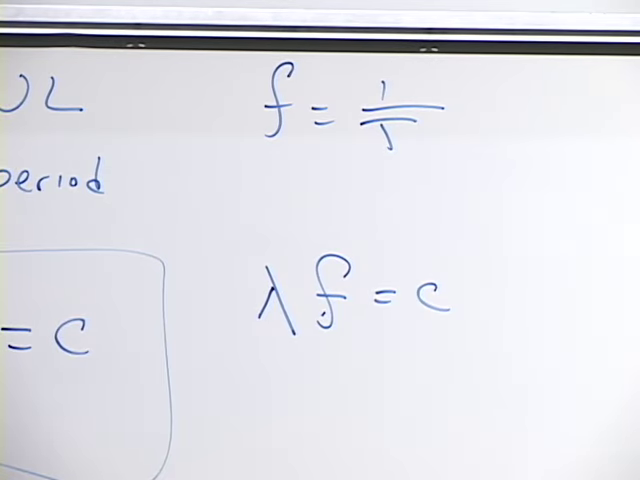
\includegraphics[width=0.68\textwidth]{lecture_01_figure_03.png}\caption{빛의 파동에서는 \(f=1/T\)이고 \(\lambda f=c\)이다.}\lectureframe{00:36:24}\end{figure}

물리학자들은 진동률을 완전한 주기의 초당 횟수 대신 초당 라디안으로 나타내는 경우가 많다. 원을 따라 등속 운동하는 상황을 생각해 보자. 어떤 점이 매초 \(f\)바퀴를 돌고, 한 바퀴가 \(2\pi\)라디안이라면 각진동수는 다음과 같다.
\begin{equation}
\omega=2\pi f,
\qquad
\frac{\omega}{2\pi}=f.
\end{equation}
지금은 이를 정의로 받아들이자. 이것이 \(2\pi\)의 인자 수를 줄여 주는지는 뒤에서 다시 살펴본다.

\(f=c/\lambda\)과 \(\omega=2\pi f\)을 결합하면 다음을 얻는다.
\begin{equation}
\omega=\frac{2\pi c}{\lambda},
\qquad
\omega\lambda=2\pi c.
\end{equation}
다른 종류의 파동에서는 \(c\) 자리에 그 파동의 전파 속력을 넣는다.

\begin{figure}[h]\centering
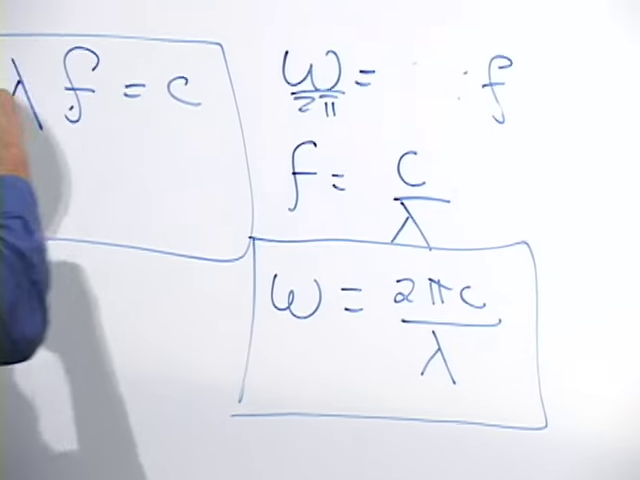
\includegraphics[width=0.68\textwidth]{lecture_01_figure_04.png}\caption{\(\omega=2\pi f\)일 때 빛의 파동은 \(\omega=2\pi c/\lambda\)을 만족한다.}\lectureframe{00:39:10}\end{figure}

전자기 복사는 연속적인 스펙트럼을 이룬다. 파장이 긴 것에서 짧은 것 순으로 배열하면 통상 다음과 같이 부른다.
\begin{equation}
\begin{aligned}
\text{radio}
&\longrightarrow \text{microwave}
\longrightarrow \text{infrared}
\longrightarrow \text{visible}\\
&\longrightarrow \text{ultraviolet}
\longrightarrow \text{X ray}
\longrightarrow \text{gamma ray}.
\end{aligned}
\end{equation}
가시광선은 이 가운데 좁은 구간만 차지한다. 각 영역의 경계는 관례에 따른 것이므로 여기서는 정확한 경계 파장이 필요하지 않다. 전파의 파장은 매우 길 수 있고, 감마선은 전자기 스펙트럼에서 파장이 가장 짧은 끝에 해당한다. 이제 어려움이 분명해졌다. 고전적으로 감마선은 연속적인 장의 파동이지만, 검출될 때는 불연속적인 깜빡임으로 나타난다.

\section{불연속적인 도달과 파동 확률}

복사의 열역학적 성질을 연구한 플랑크와 아인슈타인은 빛을 불연속적인 단위로 다루어야 한다는 결론에 이르렀다. 가상의 실험을 생각하면 그 점이 선명해지지만, 이는 실제 발견이 역사적으로 그런 경로를 따랐다는 주장이 아니다.

스크린에 빔을 비춰 보자. 보통 세기에서는 연속적으로 보이는 빛 무리가 생긴다. 빔의 일부를 가리는 감쇠기를 넣으면 빛 무리는 희미해진다. 감쇠를 거듭해서 높이면 단위 시간당 도달하는 빛의 양이 줄어든다. 그러다가 마침내 보이는 모습이 달라진다. 연속적으로 희미해진 빛 무리 대신 검출기에 고립된 사건들이 기록된다.\footnote{이 도식은 강의 영상의 00:42:32부터 00:45:42까지 전개된 감쇠 실험을 재구성한 것이다.}

\begin{figure}[h]\centering
\begin{tikzpicture}[scale=0.9]
\begin{scope}
\draw[fill=yellow!35] (0,0) circle (0.18);
\draw[->,thick] (0.2,0) -- (2.55,0);
\draw[thick] (2.65,-1.0) -- (2.65,1.0);
\node[below] at (1.4,-1.0) {\small bright beam};
\end{scope}
\begin{scope}[xshift=4.1cm]
\draw[fill=yellow!35] (0,0) circle (0.18);
\draw[->,thick] (0.2,0) -- (1.15,0);
\draw[fill=gray!70] (1.2,-0.85) rectangle (1.55,0.85);
\draw[->,thick] (1.6,0) -- (2.55,0);
\draw[thick] (2.65,-1.0) -- (2.65,1.0);
\node[below] at (1.85,-1.0) {\small strong attenuation};
\end{scope}
\fill[gray!45] (2.62,-0.65) rectangle (2.70,0.65);
\foreach \y in {-0.66,-0.31,0.13,0.58}
  \fill (6.72,\y) circle (0.045);
\node[above] at (2.65,1.0) {\small unresolved exposure};
\node[above] at (6.75,1.0) {\small isolated detections};
\end{tikzpicture}\caption{점진적으로 감쇠하면 검출률이 낮아져 연속적으로 보이는 감광이 고립된 광자 사건들로 분해된다.}\end{figure}

충분히 오래 기다리면 사건들이 쌓여 원래 빛 무리와 같은 공간 분포를 이룬다. 따라서 밝게 보였던 영역은 개별 도달 사건들이 분해되지 않은 채 합쳐진 것이었다. 이 저세기 실험은 실제로 할 수 있지만, 광자 가설의 최초 동기가 된 초기 실험은 아니었다. 아인슈타인의 광자 가설은 열역학적 고려와 광전 효과에서 비롯되었다. 감쇠 실험은 그 가설의 결과를 특히 직접적으로 떠올리게 해 준다.

이제 빔 속에 두 개의 틈을 두고 광자가 한 번에 하나씩 도달할 때까지 세기를 낮추자. 검출될 때마다 국소화된 깜빡임 하나가 기록된다. 그런데 검출이 많이 쌓이면 밝고 어두운 띠를 포함한 간섭 무늬가 채워진다. 불연속적인 도달은 무작위로 일어나지만, 그 확률 분포는 파동 무늬가 예측하는 분포와 같다. 고전적인 파동은 확률을 지배하는 파동이 되었다.

그러므로 파동과 입자는 자연의 서로 다른 부분에 각각 배정된 별개의 실체가 아니다. 둘은 같은 양자 대상이 드러내는 두 가지 모습이다. 빛을 파동으로만 또는 입자로만 적절하게 설명할 수는 없다.

전자는 처음과 반대되는 놀라움을 안겨 준다. 전자는 입자로 받아들여졌고 검출기에 한 번에 하나씩 도달하지만, 서로 가까운 틈을 두면 간섭 무늬도 만든다. 전자보다 질량이 약 팔천 배 큰 알파 입자에도 같은 원리가 적용되지만, 실험은 더 어렵다. 버키볼에서도 간섭이 관측되었다. 버키볼은 탄소 원자 육십 개가 일반화된 축구공 모양에 가깝게 배열된 분자다. 볼링공에도 같은 원리가 적용될 것으로 예상되지만, 그런 실험은 현실적으로 거의 불가능하다. 바이러스나 살아 있는 세포를 대상으로 제안된 실험까지 논의를 확장할 수도 있다. 이는 점점 더 대담한 사례들이다. 파동과 입자의 설명이 어떻게 양립하는지 이해하려면 양자역학이 필요하다. 지금 할 일은 입자물리학에 필요한 광자의 성질을 추려내는 것이다.

\section{광자 에너지}

광자는 빛을 이루는 불연속적이고 더는 나눌 수 없는 요소다. 빛은 에너지를 운반한다---햇빛은 흡수하는 물체를 데운다---따라서 광자 하나하나가 에너지를 가져야 한다. 단색파는 파장과 각진동수가 정해져 있으며, 그 파동의 광자는 모두 다음 에너지를 가진다.
\begin{equation}
E_\gamma=\hbar\omega.
\end{equation}
연속적인 파동을 작은 점들이 모인 기계적 집합으로 그려 보려는 것은 오해를 부른다. 분명한 것은 실험에서 관측되는 조합이다. 국소화된 검출 사건이 파동이 결정하는 분포에 따라 일어나고, 에너지는 나눌 수 없는 단위로 도달한다.

\begin{equation}
\omega=\frac{2\pi c}{\lambda},
\end{equation}이므로
파장이 짧을수록 각진동수가 크고 따라서 광자 하나의 에너지도 크다.
\begin{equation}
\lambda\downarrow
\quad\Longrightarrow\quad
\omega\uparrow
\quad\Longrightarrow\quad
E_\gamma\uparrow.
\end{equation}
전파 광자 하나의 에너지는 매우 작다. 하지만 전파 빔에는 광자가 아주 많이 들어 있을 수 있으므로, 빔 전체는 막대한 에너지를 운반할 수 있다. \(n\)개의 광자가 들어 있는 단색 펄스라면,
\begin{equation}
E_{\text{pulse}}=n\hbar\omega,
\qquad
n=0,1,2,\ldots.
\end{equation}
총에너지는 클 수 있지만, 여전히 광자 하나의 에너지에 정수배를 곱한 값이다.

이 관계는 앞으로 논의의 방향을 결정할 실용적인 질문으로 이어진다. 더 작은 것을 보려면 왜 점점 더 큰 기계를 만들어야 하는가? 작은 물체를 보는 데 작은 기계를 쓰면 안 되는가? 답의 전반부는 이미 나왔다. 더 작은 구조를 분해해 보려면 더 짧은 파장이 필요하고, 파장이 짧은 양자는 더 큰 에너지를 가진다.

\section{정지 에너지와 불변 질량}

입자물리학은 양자역학과 상대성이론을 결합한다. 광자 관계식 \(E_\gamma=\hbar\omega\)은 양자론 쪽을 제공하고, 상대성이론에서 대응하는 기본 사실은 다음과 같다.
\begin{equation}
E_{\mathrm{rest}}=mc^2.
\end{equation}
이때의 한정은 중요하다. 오래된 설명에서는 \emph{정지 질량}과 속도에 따라 달라지는 \emph{운동 질량}을 구별했다. 현대 용어에서 \emph{질량}은 물체의 불변 질량을 뜻한다. 운동은 에너지를 바꾸지만 질량은 바꾸지 않는다. 어떤 상태로 운동하든 전자의 질량은 모두 같지만, 전자가 가속되면 에너지는 증가한다. 따라서 이 형태의 \(E=mc^2\)은 물체 전체가 정지해 있는 기준계에서 질량을 가진 물체의 에너지를 나타낸다.

물체가 정지해 있어도 내부 구성 요소까지 정지해 있을 필요는 없다. 기체 상자는 저울 위에서 정지해 있어도 분자들은 모든 방향으로 빠르게 움직일 수 있다. 이러한 내부 운동의 에너지는 상자 전체의 정지 에너지에 포함된다. 차가운 상자에서 시작해 질량을 측정한 뒤, 상자 자체는 정지한 채 열에너지를 더해 보자. 정지 질량은 다음만큼 변한다.
\begin{equation}
\Delta m=\frac{\Delta E_{\mathrm{internal}}}{c^2}.
\end{equation}
질량이 늘어나면 무게와 관성도 커진다. 보통 상자에서는 온도를 크게 높여도 일반적인 저울로 그 효과를 알아차리기에는 너무 작다. 효과가 작다고 해서 원리가 달라지는 것은 아니다.

더 분명한 예로 전자와 양전자를 들 수 있다. 두 입자의 질량은 정확히 같고 전하는 서로 반대다. 처음에 정지해 있던 두 입자가 소멸하면 광자들이 에너지를 가져간다.
\begin{equation}
e^-+e^+\longrightarrow \text{photons}.
\end{equation}
초기 에너지는
\begin{equation}
E_{\mathrm{initial}}=2m_e c^2,
\end{equation}
이며, 그 에너지는 사라질 수 없다. 쌍 하나가 내놓는 에너지는 아주 적으므로 커피 한 잔을 데우려 해도 엄청나게 많은 쌍이 필요하다. 하지만 개별 소멸 사건은 변환을 직접 보여 준다.

따라서 정지한 물체의 질량과 에너지는 단위만 다르게 표현한 같은 물리량이다. \(c^2\)은 관습적인 질량 단위와 에너지 단위 사이의 환산 인자이며, 수를 미터에서 센티미터로 바꾸는 환산 인자와 비슷하다.

\begin{classroomqa}\lecturetimestamp{01:04:39}\audiencequestion{질량이 방출된 에너지로 바뀌려면 어떤 메커니즘이 필요한가?}\lecturerresponse{그렇다. 물리적 메커니즘이 필요하지만, 보존 법칙만으로도 그 결과에 이미 제약이 주어진다. 미시적인 소멸 메커니즘을 설명하기 전에도, 초기 전자--양전자 에너지는 어딘가에서 다시 나타나야 한다. 따라서 상호작용을 자세히 설명하지 않아도 에너지 보존으로 답의 중요한 부분을 알아낼 수 있다.}\end{classroomqa}

\section{차원과 단위의 선택}

SI 단위계에서 빛의 속력은 매우 큰 수로, 플랑크 상수는 매우 작은 수로 나타난다. 후자가 작다는 점은 광자 관계식만 보아도 알 수 있다. 가시광선의 각진동수는 엄청나게 큰 반면 광자 하나의 에너지는 매우 작으므로, 이 단위계에서 \(E_\gamma=\hbar\omega\)가 성립하려면 \(\hbar\)의 수치가 작아야 한다. 크기 차수만 나타내면 다음과 같다.
\begin{equation}
c\sim 10^8\ \mathrm{m\,s^{-1}},
\qquad
\hbar\sim 10^{-34}\ \mathrm{J\,s}.
\end{equation}
\editorialnote{칠판의 마지막 자리 숫자가 흐릿하므로 강의에서 제시한 크기 차수만 유지했다.}
단위는 필수다. 두 상수 모두 단순한 소수가 아니다. 에너지의 차원은
\begin{equation}
[E]=M L^2 T^{-2},
\end{equation}
이며, \(E_\gamma=\hbar\omega\)와 \([\omega]=T^{-1}\)를 고려하면 플랑크 상수의 차원은 다음과 같다.
\begin{equation}
[\hbar]=[E]T=M L^2 T^{-1}.
\end{equation}

\(c\)이 크고 \(\hbar\)가 작다고 말하는 것 자체가 이미 단위 선택을 전제로 한다. 속력을 시간당 피트로 재면 초당 미터로 잴 때와 \(c\)의 수치가 다르다. 광년/년이나 광초/초 단위로 나타내면 빛의 속력은 1이다. 질량, 길이, 시간 단위를 서로 맞게 선택하면 \(\hbar=1\)로 둘 수도 있다.

익숙한 단위계는 자연이 특별히 정해 둔 특성이 아니라 물려받은 관례다. 마일에는 5280피트가 들어 있고, 스톤은 14파운드이며, 말의 키는 핸드 단위로 재고, 동력은 마력으로 나타낼 수 있다. 미터법 단위는 더 체계적이지만, 그 척도 역시 인간이 선택한 것이다. 기초 물리학에는 미터, 초, 킬로그램을 특별히 지목하는 요소가 없다.

길이, 시간, 질량은 서로 독립적인 세 가지 기본 단위 선택을 이룬다.
\begin{equation}
L,\qquad T,\qquad M.
\end{equation}
다른 역학 단위는 이들로부터 만들 수 있다. 어떤 선택이 유용한지는 문제에 따라 달라진다. 천체물리학에서는 태양 질량이 편리하고, 핵물리학에서는 양성자 질량이 편리할 수 있다. 상대론적 천문학 공식은 광년과 년을 쓰면 간결해진다. 서로 독립적인 선택지가 세 가지이므로 차원이 독립적인 상수 세 개에 편리한 수치를 부여할 수 있다. 천체물리학, 원자물리학, 입자물리학은 서로 다른 선택을 해도 된다.

입자물리학에서는 다음 두 관례가 특히 유용하다.
\begin{equation}
c=1,
\qquad
\hbar=1.
\end{equation}
남은 단위에 대해서는 이에 필적할 만한 특별한 입자 질량이 없다. 양성자 질량, 힉스 보손 질량, 뮤온 질량을 1로 정할 수는 있지만, 이는 수많은 입자 가운데 하나만 특별히 취급하는 것일 뿐이다.

그렇다면 왜 \(c\)와 \(\hbar\)를 선택할까? 첫 번째 답으로는 이 값들이 여러 방정식에 나타난다는 점을 들 수 있다. 하지만 자주 등장한다는 것만으로는 충분하지 않다. 양성자 질량도 여러 방정식에 나타나며, 양성자의 크기도 마찬가지다. \(c\)와 \(\hbar\)를 구별해 주는 것은 보편성이다.

상수 \(c\)와 \(\hbar\)는 서로 다른 방식으로 보편적이다. 속력 \(c\)는 모든 물리적 대상에 제약을 가한다. 질량이 있는 물체는 이 속력에 가까워질 수 있지만, 이를 넘어서도록 가속될 수는 없다. 플랑크 상수는 다음과 같은 크기 차수의 불확정성 관계를 통해 모든 양자 대상에 제약을 가한다.
\begin{equation}
\Delta x\,\Delta p\gtrsim\hbar.
\end{equation}
두 진술 모두 특정 입자종을 따로 지정하지 않는다. 이러한 보편성 때문에 \(c=1\)와 \(\hbar=1\)를 자연스러운 관례로 삼을 수 있다.

양성자에는 이에 견줄 만한 보편적인 척도가 없다. 양성자는 많은 대상 중 하나일 뿐이다. 양성자 질량을 1로 정해도 루비듐 원자 질량을 1로 정하는 것보다 더 근본적인 의미는 없다. 전자, 힉스 보손, 뮤온을 기준으로 삼아도 같은 문제가 생긴다.

전하에서도 또 다른 보편적 물리량을 찾을 수 있을 듯하지만, \(c\)와 \(\hbar\)를 표준화하고 나면 물리적으로 중요한 전자기 결합은 무차원이다. 단위 선택으로 전자기 방정식에서 차원을 가진 상수들의 위치를 바꿀 수는 있지만, 진정한 무차원 결합의 값은 바꿀 수 없다.

중력은 차원을 가진 보편 상수를 제공한다. 뉴턴의 표현에서 두 질량 사이 힘의 크기는 다음과 같다.
\begin{equation}
F=G\frac{m_1m_2}{r^2}.
\end{equation}
모든 질량은 중력으로 상호작용하지만, 전기적으로 중성인 물체는 전기력에 참여하지 않을 수 있다. 따라서 \(G\)는 필요한 보편성을 갖는다. 그럼에도 현재 논의하는 계산에서 알려진 기본 입자 사이의 중력은 무시할 수 있으므로, 보통의 입자물리학에서 이를 실용적인 단위 기준으로 삼기는 어렵다.

\begin{classroomqa}
\lecturetimestamp{01:20:34}
\audiencequestion{\(G\)을 그저 무시해도 되는가? 매우 높은 에너지에서는 기본 입자가 여기서 가정한 방식대로 고전 중력에 따르지 않을 수도 있다.}
\lecturerresponse{개별 입자는 실제로 지구의 중력장에 반응한다. 입자 하나도 그 장 안에서 낙하한다. 한 기본 입자가 다른 기본 입자에 미치는 중력의 영향은 직접 측정된 적이 없으므로, 그 수준에서는 보편성 가정에 의문을 제기할 수 있다. \(G\)을 제외하는 직접적인 이유는 절대적인 원칙이 아니라 실용성에 있다. 중력은 일반적인 입자물리학 실험과 방정식에 무시해도 될 만큼만 기여한다.}
\end{classroomqa}

\begin{classroomqa}
\lecturetimestamp{01:22:01}
\audiencequestion{중력 대신 전자기 상호작용을 세 번째 단위 설정 규약으로 사용할 수 있을까?}
\lecturerresponse{그렇다. 전하 또는 쿨롱 법칙에 등장하는 상수를 정규화하는 전자기 단위계를 선택할 수 있다. 실제로 그런 규약을 사용한다. 전자는 서로 끌어당기는 것이 아니라 밀어내지만, 이 부호가 그런 선택을 막지는 않는다. 여기서는 단지 그 규약을 채택하지 않았을 뿐이다.}
\end{classroomqa}

\begin{classroomqa}
\lecturetimestamp{01:23:06}
\audiencequestion{\(c\)과 \(\hbar\)를 1로 두면 전하는 무차원인가?}
\lecturerresponse{그렇다. 전하의 제곱과 관련된 무차원 척도는 대략 \(1/137\)이다. 정확한 규약과 그 수의 의미는 나중에 다뤄도 된다. 여기서 중요한 점은 그 값이 무차원이라는 것이다.}
\end{classroomqa}

\begin{classroomqa}
\lecturetimestamp{01:23:37}
\audiencequestion{쿨롱 상수를 세 번째로 1로 둘 상수로 선택할 수 있을까?}
\lecturerresponse{그 상수를 전자기 단위 규약에 흡수할 수는 있다. 하지만 단위를 바꾸어도 무차원 결합 상수 \(1/137\)는 달라지지 않으므로, 그 선택으로 결합 상수를 1로 만들 수는 없다. 여기서 그 규약을 채택하는 데 특별한 이점이 있다고 주장하는 것은 아니다.}
\end{classroomqa}

\section{자연 단위계의 방정식과 기준계}

\(c=1\)를 쓰면 질량이 있는 물체의 정지 에너지 관계는 다음과 같이 된다.
\begin{equation}
E_{\mathrm{rest}}=m.
\end{equation}
\(\hbar=1\)를 쓰면 광자 관계는 다음과 같이 된다.
\begin{equation}
E_\gamma=\omega.
\end{equation}
일반적인 단위계에서 수치의 크기가 필요할 때는 언제든 상수들을 다시 넣을 수 있다.

\begin{figure}[h]
\centering
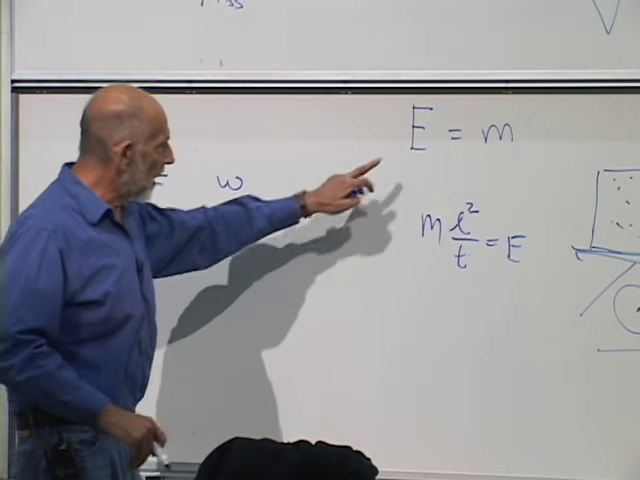
\includegraphics[width=0.72\textwidth]{lecture_01_figure_05.png}
\caption{\(c=1\)인 단위계에서 정지한 질량체의 정지 에너지는 \(E=m\)이다.}
\lectureframe{01:25:40}
\end{figure}

이 식들은 비슷해 보이지만 의미는 서로 다르다. \(E_{\mathrm{rest}}=m\)에서 \(E\)는 질량체의 정지 에너지다. 광자는 질량이 없고 정지 상태로 만들 수도 없으므로, 광자의 에너지는 정지 에너지가 아니다. 관계식 \(E_\gamma=\omega\)는 운동하는 질량 없는 양자의 에너지를 나타낸다.

\begin{classroomqa}
\lecturetimestamp{01:26:07}
\audiencequestion{정지는 언제나 어떤 대상에 대한 상대적인 상태이고 실험실 자체도 절대적으로 정지해 있지 않은데, \emph{정지}란 무슨 뜻인가?}
\lecturerresponse{정지는 선택한 기준계에 대해 정의된다. 컵이 실험실에 대해 정지해 있다면, 그 실험실 기준계에서 컵의 에너지는 \(c=1\)일 때 질량과 같으며, 전체 운동 에너지 항은 없다. 컵 곁을 지나가는 다른 관측자는 컵에 운동 에너지도 있다고 본다. 관측자마다 같은 물체나 광자에 서로 다른 에너지를 부여하는 것이 일반적이다. 에너지는 기준계에 따라 달라지며, 절대 정지를 주장할 필요는 없다.}
\end{classroomqa}

이제 각진동수 규약을 다시 살펴볼 수 있다. \(E_\gamma=\hbar\omega\)라고 쓰면 간결하지만, 앞서 \(\omega=2\pi f\)에는 \(2\pi\) 인자가 들어갔다.

\begin{classroomqa}
\lecturetimestamp{01:28:13}
\audiencequestion{초당 완전한 주기의 수라는 겉보기에 더 간단한 수 대신, 초당 라디안으로 측정하는 각진동수 \(\omega\)를 사용하는 이유는 무엇인가?}
\lecturerresponse{이 선택에는 역사적인 이유도 일부 있지만, 수학적 대답은 즉각적이라기보다 실용적인 것이다. 여기서 제시할 대답은 잠정적이다. 관련 방정식을 \(f\)를 사용해 한 번, \(\omega\)를 사용해 한 번 써 보고, 어느 규약에서 \(2\pi\) 인자가 더 적게 남는지 살펴보면 된다. 어느 쪽을 택해도 \(2\pi\) 인자가 모든 곳에서 사라지게 할 수는 없다. 복소 지수 표기법과의 연관 가능성도 제안되었지만, 여기서는 더 다루지 않는다.}
\end{classroomqa}

\begin{classroomqa}
\lecturetimestamp{01:29:51}
\audiencequestion{두 입자를 가속해 서로 간의 중력 상호작용이 중요해질 때까지 에너지를 높일 수 있을까?}
\lecturerresponse{원리적으로는 가능하다. 그러나 현재의 가속기는 실제로 그런 영역에 한참 못 미친다. 또한 답은 입자를 무엇으로 뜻하느냐에 달려 있다. 거시적인 중력체는 여기서 다루는 기본 입자와는 다른 경우다.}
\end{classroomqa}

\begin{classroomqa}
\lecturetimestamp{01:30:27}
\audiencequestion{양전자의 원천으로 무엇을 이용할 수 있는가?}
\lecturerresponse{고에너지 충돌로 양전자를 생성할 수 있다. 일부 핵 과정과 붕괴에서도 양전자가 생성된다.}
\end{classroomqa}

\begin{classroomqa}
\lecturetimestamp{01:30:53}
\audiencequestion{플랑크 시간과 플랑크 거리가 여기서 사용하는 자연 단위인가?}
\lecturerresponse{아니다. 플랑크 단위는 \(G\), \(c\), \(\hbar\)를 모두 1로 둘 때 얻어진다. 그때의 플랑크 길이는 일반적인 입자물리학의 길이 척도보다 훨씬 작으므로 여기서는 측정 기준으로 쓰기 불편하다. 중력과 양자역학, 상대론이 모두 함께 중요해지는 블랙홀 물리학, 우주론 또는 양자중력에서는 이런 단위가 자연스럽다. 중력을 무시할 수 있을 때는 \(c\)와 \(\hbar\)만 1로 두는 편이 더 유용하다.}
\end{classroomqa}

\section{운동량, 빛, 그리고 분해능}

다음 기본 개념은 운동량이다. 정지한 물체는 운동량이 없지만, 영이 아닌 정지 에너지 \(mc^2\)를 가진다. 물체가 움직이면 일반적으로 운동량을 가진다. 에너지가 보존되듯 운동량도 충돌에서 보존된다. 두 물체가 충돌할 때 충돌 전후의 전체 벡터 운동량은 같다. 보존 법칙의 제약을 받는 것은 무엇이든 특별히 주목할 만하다.

운동량은 벡터이며 운동 방향을 가리킨다. 비상대론적 물체의 경우,
\begin{equation}
\mathbf p=m\mathbf v.
\end{equation}
이는 일반적인 상대론적 공식이 아니며, 빛에 직접 적용할 수 없다.

그렇지만 빛은 에너지뿐 아니라 운동량도 가진다. 보통의 빛이 만들어 내는 미는 힘은 너무 작아 운동량을 알아차리기 어렵지만, 강한 레이저 펄스는 상당한 충격량을 전달할 수 있다. 예를 들어 리버모어의 대형 레이저는 복사가 운반하는 운동량으로 물질을 안쪽으로 밀어 넣을 수 있다.

광선이 거의 한 축을 따라 진행할 만큼 충분히 평행한 펄스를 생각해 보자. 실제 빔에는 어느 정도 각도 퍼짐이 있어 빔의 일부가 조금씩 다른 방향으로 진행할 수 있지만, 이상적으로 평행한 빔의 운동량은 빔을 따라가며 그 크기는 다음과 같다.
\begin{equation}
p=\frac{E}{c},
\qquad\text{or equivalently}\qquad
E=cp.
\end{equation}
여기서는 이 관계를 증명하기보다는 상대론적 사실로 받아들인다. 다음 차원 검사는 그 단위가 보통의 운동량 단위와 일치하는지만 확인한다.
\begin{equation}
\left[\frac{E}{c}\right]
=
\frac{M L^2 T^{-2}}{L T^{-1}}
=
M L T^{-1}
=
[m v]
=
[p].
\end{equation}
이 차원 비교는 빛에 정지 질량을 부여하지 않는다. 광자의 질량은 0이다. 광자는 에너지를 가지고 \(c\)로 움직이기 때문에 운동량을 가진다.

\(\mathbf p\)의 방향은 전파 방향이다. 분모에 \(c\)가 들어가므로 그 크기를 감지하기는 대개 어렵다. 빔은 물질을 가열하거나 증발시켜 그 에너지를 쉽게 드러낼 수 있지만, 빔이 가하는 역학적 압력은 훨씬 작다. 그러나 세기를 충분히 높이면 그 압력도 커질 수 있다.

광자 하나에 대해서는
\begin{align}
p_\gamma
&=\frac{E_\gamma}{c}\\
&=\frac{\hbar\omega}{c}.
\end{align}
이를 파장으로 나타내려면 파동 관계식을 주의 깊게 다시 살펴보자. 다음 관계에서
\begin{equation}
f\lambda=c,
\qquad
\omega=2\pi f,
\end{equation}
올바른 관계는 다음과 같다.
\begin{equation}
\omega\lambda=2\pi c,
\qquad
\omega=\frac{2\pi c}{\lambda}.
\end{equation}
정의를 써서 확인하지 않으면 \(2\pi\) 인자를 뒤집기 쉽다. \(f\lambda=c\)와 \(f=\omega/(2\pi)\)에서 다시 시작하면 문제가 명확해진다.
\begin{equation}
\frac{\omega}{2\pi}\lambda=c
\quad\Longrightarrow\quad
\omega\lambda=2\pi c.
\end{equation}
이제 대입하면 다음을 얻는다.
\begin{align}
p_\gamma
&=\frac{\hbar}{c}\frac{2\pi c}{\lambda}\\
&=\frac{2\pi\hbar}{\lambda}\\
&=\frac{h}{\lambda}.
\end{align}

\begin{classroomqa}
\lecturetimestamp{01:42:38}
\audiencequestion{\(2\pi\hbar\)는 \(h\)와 같은가?}
\lecturerresponse{그렇다. 정의에 따라 \(h=2\pi\hbar\)이므로, \(p_\gamma=2\pi\hbar/\lambda\)는 \(p_\gamma=h/\lambda\)와 같다. 어떤 진동수 규약을 선택해도 \(2\pi\) 인자는 어디엔가 다시 나타난다.}
\end{classroomqa}

파장이 짧을수록 광자의 운동량은 크다. 전파 광자는 파장이 매우 길고 운동량이 아주 작다. 감마선 광자는 파장이 매우 짧아 훨씬 큰 충격을 준다. 광자 하나가 주는 거시적인 충격량은 여전히 작지만, 전파 광자에 비하면 운동량이 훨씬 크다. \(E_\gamma=cp_\gamma\)이므로 에너지도 더 크다.

이 관계는 더 작은 물체를 관찰할수록 더 큰 장치가 필요한 이유를 설명한다. 사람 머리보다 훨씬 긴 파장의 사진으로는 흐릿한 모습만 볼 수 있다. 얼굴의 특징을 구분하려면 파장이 머리보다 짧아야 한다. 머리카락 하나를 분해하려면 파장이 머리카락의 굵기와 비슷하거나 그보다 작아야 한다. 원자의 구조를 분해하려면 탐침 파장이 원자보다 크지 않아야 한다.
\begin{equation}
\lambda_{\mathrm{probe}}\lesssim
\text{size of the structure to be resolved}.
\end{equation}
따라서 더 작은 구조를 관찰하려면 더 짧은 파장이 필요하고, 더 짧은 파장에는 더 큰 운동량과 에너지가 필요하다. 탐침이 반드시 광자여야 하는 것은 아니다. 다른 종류의 고에너지 입자에도 파장과 운동량 사이의 같은 양자적 관계가 성립한다. 그런 입자를 만들려면 입자 하나하나에 점점 더 많은 에너지를 전달하는 가속기가 필요하다. \(p_\gamma=h/\lambda\)와 \(E_\gamma=\hbar\omega\)의 관계가 이 논리를 뒷받침한다. 탐침 에너지를 높이면 운동량은 커지고 파장은 짧아진다.

대략 한 세기 동안 입자물리학에서 반복되어 온 양상은 이렇다. 에너지가 높아질수록 운동량이 커지고, 파장이 짧아지며, 공간 분해능이 높아진다.

\begin{classroomqa}
\lecturetimestamp{01:46:57}
\audiencequestion{파장에 이론적인 하한이 있을까?}
\lecturerresponse{그럴 가능성이 있다. 플랑크 길이 부근에서 새로운 현상이 나타날 것으로 예상되지만, 이는 잠정적인 답이다. 공간 분해능이 그곳에서 더는 높아지지 않는다고 해도, 그 척도는 LHC에서 탐사하는 거리보다 약 17자릿수나 작다. 따라서 현재 실험은 그 규모에 훨씬 못 미친다.}
\end{classroomqa}

같은 논리를 따라가면 가속기의 규모와 그 가속기로 분해할 수 있는 규모 사이에 대략적인 관계가 있음을 알 수 있다.

\begin{classroomqa}
\lecturetimestamp{01:48:02}
\audiencequestion{파장 또는 분해하려는 대상의 크기는 가속기의 크기에 대략 반비례하는가?}
\lecturerresponse{대략 그렇다. 다만 입자를 가속하는 최대 전기장과 입자의 진행 방향을 유도하는 자기장이 장치가 제공할 수 있는 범위 안에서 고정되어 있다고 가정해야 한다. 가속 기울기는 단위 길이당 에너지 증가량이다. 길이가 \(L\)이고 가속 기울기 \(\mathcal G\)가 대략 일정한 선형 가속기의 경우,
\[
E_{\mathrm{beam}}\sim \mathcal G L.
\]
초상대론적 에너지에서는 분해할 수 있는 파장이 에너지에 반비례하므로, 선형 가속기의 길이를 늘리면 분해능은 대략 그 역비만큼 높아진다. 이는 정확한 법칙이 아니라 경험적 규모 추정이다. 원형 가속기에서는 같은 장치를 여러 차례 통과시킬 수 있지만, 휘어지는 동안 가속된 전하가 복사를 방출해 에너지를 잃는다.}
\end{classroomqa}

\begin{classroomqa}
\lecturetimestamp{01:49:47}
\audiencequestion{플랑크 길이에 도달하려면 가속기의 크기가 어느 정도여야 하는가?}
\lecturerresponse{이 대략적인 규모 추정에 따르면 CERN의 가속기보다 약 17자릿수 더 길어야 한다. 우주의 크기까지는 아니지만, 대략 은하 규모다.}
\end{classroomqa}

\begin{classroomqa}
\lecturetimestamp{01:50:09}
\audiencequestion{최고 에너지 우주선의 에너지는 충돌기 에너지와 어떻게 비교되는가?}
\lecturerresponse{개별 우주선의 실험실 에너지는 훨씬 클 수 있다. 수치로 비교하기 위해 실험실 에너지가 대략 \(10^{21}\,\mathrm{eV}=10^{12}\,\mathrm{GeV}\)인 극단적인 우주선을 생각해 보자. 그러나 우주선은 실험실에서 정지해 있는 표적을 때리는 반면, 충돌기에서는 에너지가 큰 두 빔을 정면으로 충돌시킨다. 더 중요한 점은 유용한 실험에는 입자속, 즉 많은 입자와 잘 제어된 많은 충돌이 필요하다는 것이다. 우주선 하나는 관련 표적을 빗나갈 수도 있고, 무엇을 추론하기 어려운 사건을 만들 수도 있다. 유용한 은하 규모 가속기를 가동하는 데 필요한 전력을 석유 소비량으로 바꾸어 과장되게 추산한 결과, 초당 약 100조 배럴의 석유가 필요하다는 값이 제시되었다. 이 추산의 요지는 충분한 충돌 통계를 확보하는 일이 가속기의 길이만큼이나 심각한 장애물임을 보이는 데 있다.}
\end{classroomqa}

\editorialnote{석유 환산 추산은 원문에서 일관되지 않는다. 처음 제시한 뒤 초당 약 \(10^{14}\)배럴이라고 반복하지만, 나중에 다시 언급할 때는 초당 \(10^{11}\)배럴이라고 한다. 두 규모를 모두 남겨 두고 임의로 조정하지 않았다.}

이 거리 척도는 단지 형식적인 것이 아니라 실제로 존재한다. 실질적인 난제는 은하 규모의 가속기를 만들고 그 막대한 전력을 공급하지 않고도 그런 척도를 어떻게 탐사할 것인가이다.

\begin{classroomqa}
\lecturetimestamp{01:52:55}
\audiencequestion{LHC의 에너지는 \(10^{12}\,\mathrm{GeV}\) 에너지의 우주선과 어떻게 비교해야 하는가?}
\lecturerresponse{실험실에서 에너지가 \(E_{\mathrm{lab}}\)인 초상대론적 입사 입자가 질량 \(m_{\mathrm{target}}\)인 고정 표적을 때릴 때, 질량중심 에너지는 매개변수적으로 다음과 같이 주어진다.
\[
E_{\mathrm{cm}}\simeq
\sqrt{2m_{\mathrm{target}}c^2E_{\mathrm{lab}}}.
\]
\editorialnote{고정 표적 식을 표시해, 이 문답에서 언급한 제곱근에 비례하는 관계를 명시했다.}
표적 질량을 고정하면 유용한 충돌 에너지는 입사 입자 에너지의 제곱근만큼만 증가한다. 따라서 \(10^{12}\,\mathrm{GeV}\) 에너지의 우주선은 규모 추정상 서로 반대 방향으로 진행하는 빔 각각의 에너지가 \(10^6\,\mathrm{GeV}\) 정도인 경우에 해당하며, 각 빔이 \(10^{12}\,\mathrm{GeV}\)인 경우에 해당하지 않는다. 우주선의 에너지는 여전히 지상 충돌기의 에너지를 넘어설 수 있지만, 우주선의 속이 매우 낮아 체계적이고 통제된 실험에는 적합하지 않다.}
\end{classroomqa}
\chapter{파동, 양자화된 모드와 생성 연산자}

\section{파동, 장과 복소 지수함수}

양자장론은 입자물리학의 기본 도구다. 양자장을 기초 수준에서 다루기 전에도, 파동과 입자를 이어 주는 수학적 사실들을 정리해 두면 유용하다. 파동은 이미 장의 한 배치다. 장은 공간의 각 점에서 값이 달라지며, 파동은 그 값들이 진동하며 전파되는 배치다. 양자역학은 이러한 파동과 입자를 연결해 준다.

여기서는 양자역학과 특수상대성이론을 이미 배운 것으로 전제한다. 당장의 목적은 입자물리학에 필요한 내용을 복습하는 것이지, 두 과목 가운데 어느 하나를 대신하는 것이 아니다.

지수함수는 비례하는 증가로 특징지어진다. \begin{equation}
f(x)=e^{\alpha x},
\end{equation}그러면 \begin{equation}
\frac{df}{dx}=\alpha f.
\end{equation}짧은 구간에서 증가량은 이미 존재하는 양에 비례한다. 페트리 접시에서 개체군이 증가하는 경우를 생각하면 익숙한 그림이 된다. 생물이 많을수록 번식할 개체도 많아지므로, 증가율은 개체군 자체에 비례한다. \(e^{\alpha x}\)에 전체 상수를 곱해도 이 정의적 성질은 달라지지 않는다.

사인과 코사인은 증가하는 대신 진동한다. 두 함수는 주기의 사분의 일만큼 이동한 같은 곡선이며, 미분하면 서로 변환된다:
\begin{align}
\frac{d}{dx}\sin(kx)&=k\cos(kx),\\
\frac{d}{dx}\cos(kx)&=-k\sin(kx).
\end{align}
두 함수 중 어느 하나도 단독으로는 지수함수가 아니다. 그 도함수가 다른 함수에 비례하기 때문이다. 두 함수를 복소수로 결합하면 지수함수의 성질을 갖는다. \(i^2=-1\)일 때,
\begin{align}
\frac{d}{dx}\bigl(\cos(kx)+i\sin(kx)\bigr)
&=-k\sin(kx)+ik\cos(kx)\\
&=ik\bigl(\cos(kx)+i\sin(kx)\bigr).
\end{align}
따라서
\begin{equation}
e^{ikx}=\cos(kx)+i\sin(kx).
\end{equation}
사인과 코사인은 파동과 같은 진동을 나타내므로 이 항등식은 반복해서 등장한다. \(x\)가 공간 좌표이면 함수는 공간에 따라 진동한다. 논항이 시간이면 시간에 따라 진동한다.

\section{진동수, 파장과 광자 운동량}

보통 진동수 \(f\)는 1초 동안의 완전한 주기 수다. 주기란 한 번의 완전한 진동을 뜻한다. 각진동수는 같은 운동을 초당 라디안으로 나타낸다. \begin{equation}
\omega=2\pi f.
\end{equation}두 표기법은 같은 진동수를 나타낸다. 불필요한 \(2\pi\) 인자가 계산에 들어가지 않도록 둘 사이를 오가지만, 이 인자들이 완전히 사라지는 것은 아니다.

파장 \(\lambda\)은 공간에서 한 번의 완전한 주기가 차지하는 거리다. 파동이 속력 \(v\)로 전파된다면, 주기당 거리와 초당 주기 수를 곱한 값이 전파 속력이다. \begin{equation}
\lambda f=v.
\end{equation}진공에서 빛은 \(v=c\)이므로, \begin{equation}
\lambda f=c.
\end{equation}음파에서는 우변이 음속이고, 물결파에서는 해당 물결파의 속력이다. 그러므로 \(c\)가 나타나는 것은 빛에 관한 진술이지 모든 파동에 공통인 정의가 아니다.

양자역학에서는 플랑크 상수를 두 가지 표기로 쓴다. \begin{equation}
\hbar=\frac{h}{2\pi}.
\end{equation}\(h\)에서 \(\hbar\)로 바꾸는 것은 \(2\pi\) 인자를 한 방정식에서 다른 방정식으로 옮기는 것뿐이다.

차원을 가진 상수의 수치는 어떤 단위를 쓰느냐에 따라 달라진다. 미터, 초, 킬로그램은 일상적인 길이와 시간을 나타내기에 편리한 인간 규모의 관습적 단위다. 팔 길이와 비슷한 전통 단위는 천이나 밧줄을 재는 데 유용했다. 미터가 정확히 어떤 역사적 경로를 거쳐 정해졌든, 이 특정한 인간 규모를 선택하는 근본 원리는 없다. SI 단위에서는 \begin{equation}
\begin{aligned}
h &\simeq 6.6\times10^{-34}\ \mathrm{J\,s},
&\hbar &\simeq 1.1\times10^{-34}\ \mathrm{J\,s},\\
c &\simeq 3\times10^8\ \mathrm{m\,s^{-1}}.
\end{aligned}
\end{equation}이 수치들이 보여 주는 것은 관습적 단위로 나타낸 규모다. 플랑크 상수는 극도로 작고 빛의 속력은 극도로 크다.

한 모드의 양자 하나가 갖는 에너지는 \begin{equation}
E_{\text{one quantum}}=\hbar\omega=hf.
\end{equation}이다. 이는 광자 하나의 에너지이지, 임의의 고전적 전자기파 전체의 에너지가 아니다. 가시광선의 진동수는 초당 \(10^{15}\)주기 정도이므로, 전형적인 광자 하나의 에너지는 \begin{equation}
E_\gamma\sim 10^{-19}\ \mathrm{J}.
\end{equation}정도다. \(h\)가 매우 작기 때문에, 이렇게 빠른 광학적 진동도 양자 하나당 에너지는 매우 작다. 따라서 거시적인 양의 광학 에너지에는 엄청나게 많은 광자가 들어 있다.

에너지와 운동량은 둘 다 보존되므로 특별히 주의를 기울일 만하다. 두 양은 유용한 장부상의 물리량이다. 과정에 들어가는 전체 에너지와 운동량은 그 과정에서 나가는 전체 에너지와 운동량으로 균형을 이루어야 한다. 운동량은 벡터이며 운동 방향을 향한다. 빛보다 훨씬 느리게 움직이는 입자의 경우, \begin{equation}
\vec p=m\vec v.
\end{equation}

이번에는 여러 방향으로 퍼지지 않고 한 방향을 따라 평행하게 진행하는 전자기 복사를 생각하자. 그 운동량은 빔을 따라 향한다. \(m\)은 정지 질량을 뜻하고 광자의 정지 질량은 0이므로, 비상대론적 공식을 광자에 적용할 수는 없다. 그래도 차원에 관한 유용한 기억법은 있다. 광자에 \emph{부적절하게} 질량인 것처럼 \(E/c^2\)라는 양을 부여한 뒤 \(v=c\)를 대입하면, \begin{equation}
mv\longrightarrow \frac{E}{c^2}c=\frac{E}{c}.
\end{equation}이 방법은 우연히 올바른 답을 주고 단위도 맞지만, 광자의 정지 질량이 \(E/c^2\)라고 주장하는 정당한 논증은 아니다. 평행한 복사에 대한 실제 상대론적 진술은 \begin{equation}
|\vec p|=\frac{E}{c}.
\end{equation}이다. 이 방정식은 크기를 준다. 방향은 복사가 진행하는 방향이다.

광자 하나에 대해서는 \begin{align}
|\vec p_\gamma|
&=\frac{E_\gamma}{c}
=\frac{hf}{c}.
\end{align}이다. 빛의 경우, \begin{equation}
\lambda f=c,
\qquad
\frac{f}{c}=\frac{1}{\lambda},
\end{equation}\begin{equation}
|\vec p_\gamma|=\frac{hf}{c}=\frac{h}{\lambda}.
\end{equation}이므로,

\begin{figure}[t]\centering
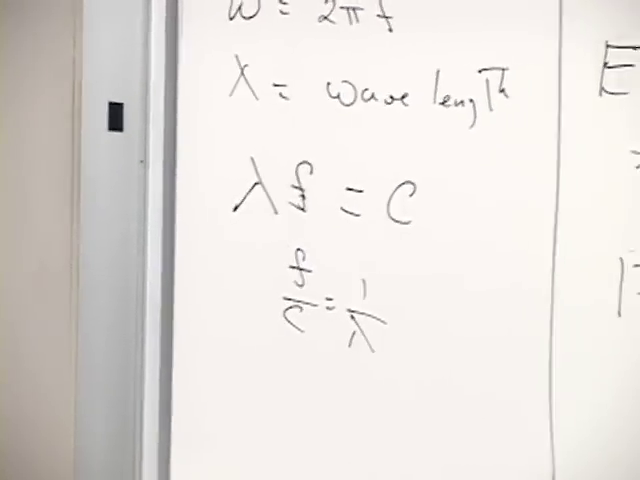
\includegraphics[width=0.56\textwidth]{lecture_02_figure_02.png}\caption{빛의 경우 \(\lambda f=c\)와 \(f/c=1/\lambda\)를 이용해 \(|\vec p_\gamma|=h/\lambda\)를 얻는다.}\lectureframe{00:21:39}\end{figure}

파장이 짧을수록 광자의 운동량은 커진다. 이것은 입자물리학에서 가장 중요한 양자적 사실 가운데 하나다. 작은 물체를 연구하려면 파장이 짧은 탐침이 필요하며, 파장을 짧게 하기 위해 치러야 하는 대가가 큰 운동량이다.

\begin{classroomqa}\lecturetimestamp{00:22:23}\audiencequestion{\(E=\hbar\omega\)은 근본적인가, 아니면 더 깊은 원리에서 유도되는가?}\lecturerresponse{조화진동자의 양자역학에서 나온다. 그 결과는 증명을 되풀이하지 않고 여기서 사용하겠다. 아래에서 다룰 진동자 표현을 통해 그 결과가 놓인 더 깊은 맥락을 살펴볼 수 있다.}\end{classroomqa}


\section{파동의 진폭과 광자 수}

\begin{classroomqa}\lecturetimestamp{00:23:10}\audiencequestion{광자의 관점에서 파동의 진폭은 무엇을 뜻하는가?}\lecturerresponse{진동수와 파장은 같지만 진폭은 다른 두 파동, 이를테면 \(\sin(kx)\)과 \(A\sin(kx)\)를 비교해 보자. 고전적으로 고정된 영역 안의 에너지는 진폭의 제곱에 비례한다. 양자역학적으로 \(n\)개의 광자를 포함한 모드의 에너지는 \(n\hbar\omega\)다. 따라서 진동수와 영역, 정규화를 고정하면 진폭의 크기는 대략 \(\sqrt n\)에 따라 커진다.}\end{classroomqa}

두 파동은 진동 양상이 같다. 한쪽이 단지 다른 쪽보다 더 강할 뿐이다.\footnote{도식은 00:23:47--00:24:28의 파동 비교를 따른다.}

\begin{figure}[t]\centering
\begin{tikzpicture}[x=1cm,y=0.65cm]
\draw[->] (-0.4,0) -- (6.8,0);
\draw[->] (-0.4,-2.1) -- (6.8,-2.1);
\draw[thick] plot[domain=0:6.2,samples=120] (\x,{0.45*sin(\x r)});
\draw[thick] plot[domain=0:6.2,samples=120] (\x,{-2.1+1.15*sin(\x r)});
\draw (6.2,0.55) node[right]{small amplitude};
\draw (6.2,-0.75) node[right]{large amplitude};
\end{tikzpicture}\caption{파장과 진동수는 같고 진폭은 다른 파동.}\end{figure}

파동의 양을 고정하면, \begin{equation}
E_{\text{wave}}\propto A^2.
\end{equation}전자기파의 경우 이는 장의 에너지가 장의 세기 제곱에 비례한다는 익숙한 진술이다. 같은 모드에 \(n\)개의 광자가 들어 있다면, \begin{equation}
E_{\text{wave}}=n\hbar\omega.
\end{equation}따라서 모드와 진동수, 정규화, 영역을 고정했을 때, \begin{equation}
A^2\propto n\hbar\omega,
\qquad
A\propto\sqrt n\quad\text{at fixed }\omega.
\end{equation}정확한 정규화를 주장하는 것은 아니다. 포함된 파동의 양이 중요하다. 균일한 파동의 길이를 두 배로 하면 국소 진폭은 그대로지만 전체 에너지는 달라진다. 그러므로 이 비례 관계는 한 파장과 같은 고정된 영역에 대해 이해할 수 있다.

여기에는 양자역학 특유의 단서도 있다. 진폭과 위상에 동시에 고전적인 정확한 값을 지정할 수는 없다. 따라서 완벽하게 확정된 고전적 장을 묻는 것이라면 ``광자 하나의 진폭은 얼마인가?''라는 질문은 모호하다. 그럼에도 \(n=1\)로 두면 크기를 추정하는 합리적인 기준을 얻을 수 있다.

\begin{classroomqa}\lecturetimestamp{00:28:25}\audiencequestion{전자기파 그림에서 수직 변위는 공간 속 광자의 위치를 나타내는가?}\lecturerresponse{아니다. 전파축은 공간 방향이고, 수직 좌표는 전기장이나 자기장의 값을 나타낸다. 운동량은 전파축 방향을 향하며, 그래프에 표시된 장의 진폭 방향을 향하지 않는다.}\end{classroomqa}

파동은 어느 공간 방향으로든 전파될 수 있지만, 익숙한 사인파 그림에서는 수평축만 공간 좌표로 사용한다. 그래프의 다른 축은 장의 세기를 나타낸다.

\begin{classroomqa}\lecturetimestamp{00:29:37}\audiencequestion{파동의 광자 수는 파동의 한 파장이나 한 주기 안에 들어 있는 수를 세는 것인가?}\lecturerresponse{한 파장처럼 고정된 영역을 택할 수 있다. 비례 관계만 성립하는 이유가 여기에 있다. 전체 에너지와 광자 수도 파동에서 얼마나 많은 부분을 포함하느냐에 따라 달라진다. 진폭이 같아도 두 파장, 세 파장, 네 파장에 들어 있는 에너지는 한 파장에 들어 있는 에너지보다 그에 비례해 크다.}\end{classroomqa}

\begin{classroomqa}\lecturetimestamp{00:30:17}\audiencequestion{광자 하나의 진폭은 의미가 없는가?}\lecturerresponse{\(n=1\)로 두어 얻는 크기 추정으로만 의미가 있다. 전자기 모드에서 전기장과 자기장 정보는 서로 켤레인 위치와 운동량 정보에 유사한 역할을 하므로, 양자 불확정성이 고전적 진폭을 얼마나 정확히 지정할 수 있는지 제한한다. 그래도 크기 추정 관계는 유용하다.}\end{classroomqa}

이 질문들은 장 변수와 입자 수의 관계를 정확히 서술할 수 있는 양자장론으로 이어진다. 지금은 비례 관계만으로 충분하다.

\section{일반적인 양자 관계와 느린 물질파}

광자에 대해 도입한 몇몇 공식은 훨씬 더 일반적으로 적용되지만, 그렇지 않은 공식도 있다. 전자로 넘어가기 전에 이를 구분해 두자.

\begin{figure}[t]\centering
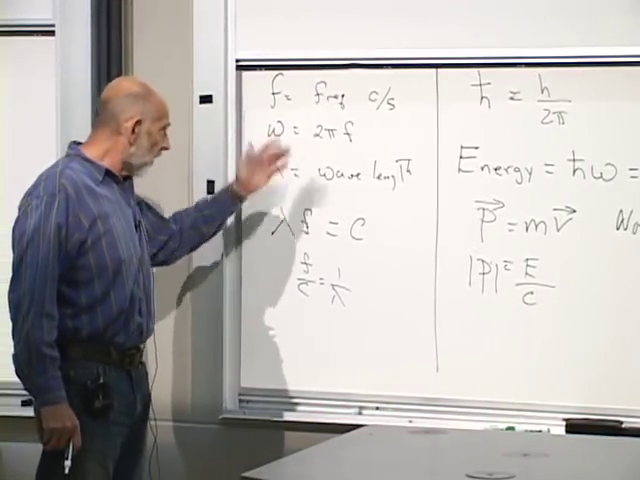
\includegraphics[width=0.82\textwidth]{lecture_02_figure_03.png}\caption{파동의 정의, 광자 운동량 관계와 비상대론적 운동량 관계의 적용 범위 비교.}\lectureframe{00:31:52}\end{figure}

\(f\), \(\omega=2\pi f\), \(\lambda\)의 정의는 일반적으로 적용된다. 이 논의에서 양자 관계 \begin{equation}
E=\hbar\omega=hf
\end{equation}도 일반적으로 성립한다. 반면 \(c\)가 포함된 공식, 예를 들어 \(\lambda f=c\)과 \(|\vec p|=E/c\)는 빛의 속력으로 움직이는 파동에 적용된다. 공식 \(\vec p=m\vec v\)은 빛보다 훨씬 느리게 움직이는 입자에 적용된다. 이 두 극한 사이의 상대론적 운동을 다루려면 보간 관계가 필요하지만, 아직은 필요하지 않다.

운동량--파장 관계는 광자의 예를 넘어 성립한다. \begin{equation}
p=\frac{h}{\lambda}.
\end{equation}여기서 \(p\)은 \(\lambda\)를 양의 파장으로 취했을 때 그 크기를 뜻한다. 방향은 따로 지정할 수 있다.

\begin{figure}[t]\centering
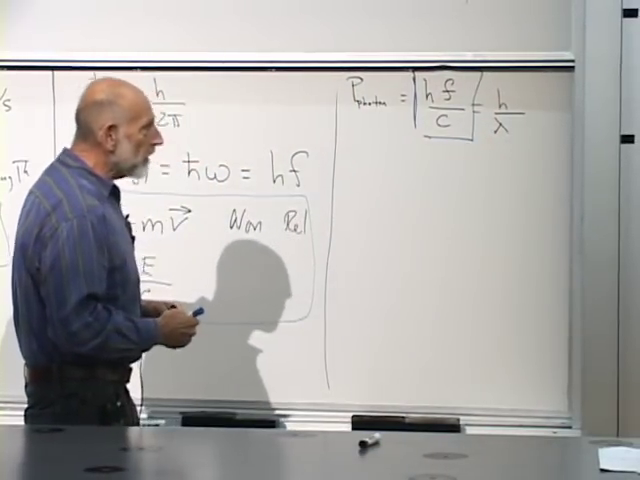
\includegraphics[width=0.74\textwidth]{lecture_02_figure_04.png}\caption{광자 운동량 \(|\vec p_\gamma|=hf/c=h/\lambda\)에서 일반적인 드브로이 관계로 이어진다.}\lectureframe{00:33:32}\end{figure}

전자, 원자핵은 물론이고 볼링공에도 파동을 대응시킬 수 있다. 전자 간섭은 그 사실이 드러나는 한 가지 사례다. 전자파를 \(\psi\)라 쓰자. 느리게 움직이는 전자에 대해서는 무엇이 \(\lambda f=c\)를 대신할까? 빠진 요소는 에너지와 운동량 사이의 비상대론적 관계다.

운동 에너지와 운동량에서 시작하자. \begin{align}
E&=\frac12 mv^2,\\
p&=mv,
\qquad
v=\frac{p}{m}.
\end{align}마지막 관계를 첫 번째 관계에 대입하면 \begin{align}
E
&=\frac12m\left(\frac{p}{m}\right)^2\\
&=\frac{p^2}{2m}.
\end{align}질량은 \(\frac12 mv^2\)에서는 분자에, \(p^2/(2m)\)에서는 분모에 놓인다. 이 위치는 혼동하기 쉬우므로 직접 다시 유도해 볼 만하다.

이제 일반적인 양자 관계를 쓰자. \begin{equation}
E=hf,
\qquad
p=\frac{h}{\lambda}.
\end{equation}느린 입자 하나에 대해서는, \begin{align}
hf
&=\frac{p^2}{2m}\\
&=\frac{1}{2m}\left(\frac{h}{\lambda}\right)^2\\
&=\frac{h^2}{2m\lambda^2}.
\end{align}\(h\)으로 나누면, \begin{equation}
f=\frac{h}{2m\lambda^2}.
\end{equation}

\begin{figure}[t]\centering
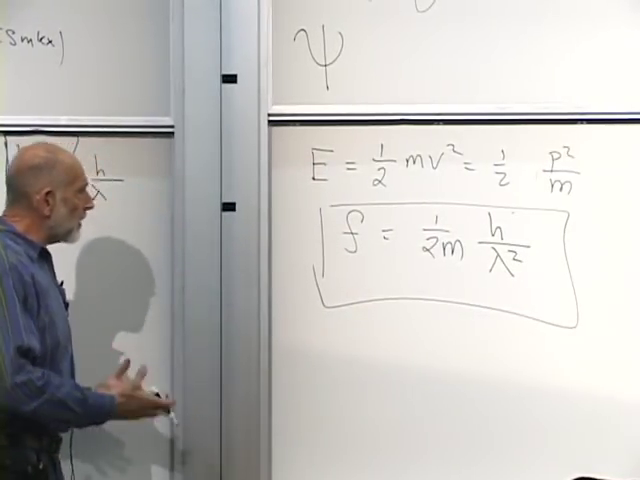
\includegraphics[width=0.64\textwidth]{lecture_02_figure_05.png}\caption{느린 입자에서는 \(E=p^2/(2m)\)과 \(p=h/\lambda\)로부터 \(f=h/(2m\lambda^2)\)을 얻는다.}\lectureframe{00:37:47}\end{figure}

빛의 경우, \begin{equation}
f\propto\frac{1}{\lambda},
\end{equation}인 반면 느린 물질의 경우, \begin{equation}
f\propto\frac{1}{\lambda^2}.
\end{equation}다. 두 번째 관계만 따로 외울 필요는 없다. \(E=p^2/(2m)\), \(E=hf\), \(p=h/\lambda\)에서 언제든 다시 유도할 수 있다. 원자 안에서 느리게 움직이는 전자에 적용하면, 이에 대응하는 Schr\"odinger 파의 진동수를 얻는다.

\begin{classroomqa}\lecturetimestamp{00:38:35}\audiencequestion{비상대론적 진동수--파장 관계는 전자 이외의 입자에도 적용되는가?}\lecturerresponse{그렇다. 빛보다 훨씬 느리게 움직이는 모든 입자에 적용된다. 느린 극한과 빛과 같은 극한 사이의 상대론적 보간은 별개의 주제다.}\end{classroomqa}

\begin{classroomqa}\lecturetimestamp{00:38:55}\audiencequestion{중성미자에는 어떤 관계를 적용해야 하는가?}\lecturerresponse{중성미자의 속력에 따라 다르다. 자연에서 만나는 중성미자의 대부분은 빛의 속력에 매우 가까운 속력으로 움직이므로 빛과 같은 극한의 관계가 좋은 근사다. 빛보다 훨씬 느리게 움직이는 중성미자라면 비상대론적 관계를 따라야 한다.}\end{classroomqa}

\editorialnote{중성미자 질문 직후에 오간 짧은 청중 문답은 진폭, 양자, 서로 다른 전자 파장을 다루지만, 발언이 심하게 손상되어 정확히 복원하기 어렵다. 복원 가능한 답변에서는 파장이 다른 경우의 진폭과 양자 사이의 일반 관계에 대한 논의를 뒤로 미룬다.}

\begin{classroomqa}\lecturetimestamp{00:39:56}\audiencequestion{가속기에서 나온 \(20\,\mathrm{keV}\) 전자는 느린가, 상대론적인가?}\lecturerresponse{느린 입자로 취급한다. \(c=1\)인 단위계에서는 질량, 에너지, 운동량을 같은 단위로 나타낼 수 있다. 전자의 정지 에너지 규모는 대략 \(0.5\,\mathrm{MeV}\)인 반면, \(20\,\mathrm{keV}\)는 이보다 훨씬 작다. 비상대론적 운동량 기준으로 쓰면 \(p\ll mc\)이다.}\end{classroomqa}

예제의 에너지 비교는 다음과 같다. \begin{equation}
K=20\,\mathrm{keV}\ll m_ec^2\simeq0.5\,\mathrm{MeV}.
\end{equation}\editorialnote{00:39:56--00:41:40의 원문 구절에서는 \(20\,\mathrm{keV}\)를 가속기 에너지로 제시한 다음, 상대론적 기준을 운동량과 정지 질량의 비교로 표현한다. 제시된 에너지를 운동량과 동일시하지 않으면서 비상대론적이라는 결론을 유지하려면 운동 에너지 기준과 운동량 기준을 따로 쓰면 된다.}

\section{위상 속도, 군속도와 분산}

\begin{classroomqa}\lecturetimestamp{00:41:46}\audiencequestion{진동수와 파장을 곱해 전자파의 속도를 구할 수 있는가?}\lecturerresponse{그렇게 얻는 것은 위상 속도이지 전자에 대응시키는 속도가 아니다. 국소화된 파동 묶음에는 내부 마루와 골의 운동을 나타내는 위상 속도와 포락선의 운동을 나타내는 군속도가 모두 있다. 군속도를 입자의 운동과 동일시한다.}\end{classroomqa}

파동 묶음은 국소적으로 사인파나 코사인파처럼 보이지만 포락선 안에 국한되어 있다. 파동 묶음이 움직일 때 포락선과 그 안의 마루가 같은 속력으로 움직일 필요는 없다.\footnote{도식은 00:42:34--00:44:11의 파동 묶음 논의를 따른다.}

\begin{figure}[t]\centering
\begin{tikzpicture}[x=0.75cm,y=0.8cm]
\draw[->] (-0.5,0) -- (12.8,0);
\draw[thick] plot[domain=0:12,samples=140] (\x,{1.10*exp(-0.20*(\x-6)^2)});
\draw[thick] plot[domain=0:12,samples=140] (\x,{-1.10*exp(-0.20*(\x-6)^2)});
\draw[thick] plot[domain=0:12,samples=240] (\x,{1.10*exp(-0.20*(\x-6)^2)*sin(6*\x r)});
\draw[->] (4.1,1.45) -- (7.5,1.45);
\draw (5.8,1.8) node{group motion};
\draw[->] (7.0,-1.55) -- (8.3,-1.55);
\draw (8.7,-1.55) node[right]{phase motion};
\end{tikzpicture}\caption{포락선과 내부 위상이 일반적으로 서로 다른 속도로 움직이는 국소화된 파동 묶음.}\end{figure}

위상 속도는 단색 성분의 마루와 골, 그리고 다른 고정된 위상점들의 속도다. 비상대론적 분산 관계에서는, \begin{equation}
v_\phi=f\lambda=\frac{h}{2m\lambda}.
\end{equation}파장에 따라 달라진다. 따라서 파장이 다른 성분들은 위상 속도도 서로 다르고, 마루는 파동 묶음 안을 지나가며 파동 묶음은 분산될 수 있다. 군속도는 파동 묶음 전체의 속도이며, 입자의 속도와 동일시하는 값이다.

간단한 특수한 경우가 있다. 모든 파장 성분이 같은 속도로 움직이면 위상 속도와 군속도가 일치한다. 진공 속 빛은 이러한 성질을 갖는다. 모든 파장이 \(c\)의 속력으로 전파된다. 느린 입자에 대한 관계는 그렇지 않으며, 그 관계에서 \(f\lambda\)는 \(\lambda\)에 따라 달라진다.

방정식 \begin{equation}
f=\frac{h}{2m\lambda^2}
\end{equation}은 자유 Schr\"odinger 방정식을 조금 다른 형태로 쓴 것이다. 진동수는 평면파의 시간 의존성을, 파장은 공간 의존성을 정하며, Schr\"odinger 방정식은 두 의존성을 연결한다. 반대로, 진동수와 파장이 정해진 파동을 자유 Schr\"odinger 방정식에 대입해도 이 분산 관계를 얻는다.

\begin{classroomqa}\lecturetimestamp{00:47:02}\audiencequestion{위상 속도가 빛의 속력을 초과할 수 있는가?}\lecturerresponse{그렇다. 위상 속도는 정보를 전달하지 않는다. 정보와 국소화된 파동 묶음은 군속도로 전파되므로, 위상 속도가 광속보다 빠르더라도 광속보다 빠른 신호 전달이 가능해지는 것은 아니다.}\end{classroomqa}

\section{유한한 공간과 이산 운동량}

궁극적인 관심은 무한 공간의 파동에 있지만, 유한한 계에서 시작하는 편이 더 안전하다. 무한대는 컴퓨터가 직접 저장하거나 조작할 수 있는 것이 아니다. 먼저 유한한 계에 대한 방정식을 세우고 나서, 계의 크기를 한없이 크게 만드는 극한을 취한다. 이 습관은 양자역학, 양자장론, 입자물리학 전반에서 유용하다.

한 공간 차원에서 시작해도 본질적인 것을 잃지 않는다. 파동은 바이올린 줄이나 흔들리는 밧줄 위에 있을 수도 있고, 추상적인 1차원 세계에 있을 수도 있다. 가장 명백한 유한계는 길이 \(L\)인 선분과 그 양 끝의 반사 경계다. 파동은 한쪽 끝까지 가서 반사된 뒤 되돌아온다. 이는 완전히 타당한 반사 경계 조건이지만 한 가지 불편함이 있다. 파동계 안에서 운동량이 보존되지 않는다. 오른쪽으로 진행하는 파동은 오른쪽 방향의 운동량을 가진다. 반사된 뒤에는 왼쪽 방향의 운동량을 가진다. 경계가 충격량을 가하고 그 차이를 흡수한 것이다.

반사 경계에서 운동량이 뒤집히는 모습을 도식으로 나타낼 수 있다.\footnote{도식은 00:49:24--00:51:08의 반사 경계 논의를 따른다.}

\begin{figure}[t]\centering
\begin{tikzpicture}[x=1cm,y=1cm]
\draw[thick] (0,0) -- (7,0);
\draw[very thick] (0,-0.45) -- (0,0.45);
\draw[very thick] (7,-0.45) -- (7,0.45);
\draw[->,thick] (1.0,0.35) -- (5.8,0.35) node[midway,above]{\(p>0\)};
\draw[->,thick] (5.8,-0.35) -- (1.0,-0.35) node[midway,below]{\(p<0\)};
\draw (3.5,-0.85) node{\(L\)};
\end{tikzpicture}\caption{유한한 선분의 양 끝에서 반사되면 진행하는 파동의 운동량이 반전된다.}\end{figure}

운동량을 보존하면서 계를 유한하게 만드는 다른 방법이 있다. 선분의 두 끝점을 서로 동일시하는 것이다. 그 결과를 원으로 그릴 수는 있지만, 2차원 공간 안에 실제 원이 놓여 있어야 하는 것은 아니다. 수학적으로는 좌표가 주기적이라는 뜻이다. 총 거리 \(L\)만큼 이동한 뒤에는 같은 점으로 돌아온다.

\begin{figure}[t]\centering
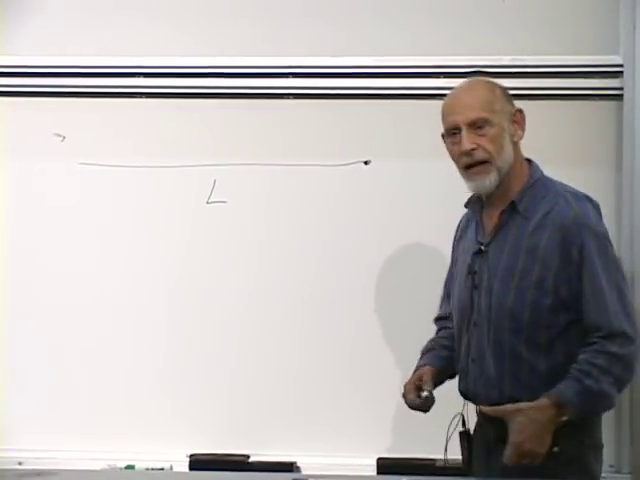
\includegraphics[width=0.72\textwidth]{lecture_02_figure_06.png}\caption{길이 \(L\)인 경로를 주기적으로 동일시하는 방법을 소개한다.}\lectureframe{00:51:21}\end{figure}

다음 도식에서 끝점의 동일시를 명시적으로 나타낸다.\footnote{도식은 00:51:09--00:52:37의 주기적 동일시 논의를 따른다.}

\begin{figure}[t]\centering
\begin{tikzpicture}[x=1cm,y=1cm]
\draw[thick] (0,0) -- (7,0);
\fill (0,0) circle (1.5pt);
\fill (7,0) circle (1.5pt);
\draw[->,thick] (1.0,0.35) -- (6.0,0.35);
\draw (3.5,-0.35) node{\(L\)};
\draw[->,bend left=45] (7,0.08) to (0,0.08);
\draw (3.5,1.2) node{identified endpoints};
\end{tikzpicture}\caption{길이 \(L\)인 경로의 양 끝점을 동일시해 만든 주기적인 1차원 공간.}\end{figure}

그러면 오른쪽으로 가는 파동은 그림에 표시된 끝점에 도달한 뒤 처음으로 다시 나타나 계속 오른쪽으로 진행한다. 왼쪽으로 가는 파동도 계속 왼쪽으로 진행한다. 파동이 반사되는 특별한 끝점이 없으므로 운동량은 반전되지 않는다. 주기적 공간은 부피를 유한하게 유지하면서 운동량을 보존하지만, 중요한 결과가 따른다. 허용되는 운동량이 이산적이다.

정수 개의 파장이 전체 길이에 들어맞아야 한다. 상수가 아닌 모드의 경우, \begin{equation}
\lambda_{|N|}=\frac{L}{|N|},
\qquad |N|=1,2,3,\ldots .
\end{equation}따라서 파장의 크기는 \(L\), \(L/2\), \(L/3\) 등일 수 있다. \(L/\sqrt{2}\)와 같은 선택은 들어맞지 않는다. 한 바퀴 돈 뒤 파동이 위상이 맞지 않는 채 돌아와 시작점의 값과 일치하지 않기 때문이다.

\(p=h/\lambda\)을 이용하면 \(|N|\)번째 비상수 모드의 운동량 크기는
\begin{equation}
|p_N|=\frac{|N|h}{L}.
\end{equation}
양방향과 상수 모드를 모호함 없이 모두 포함하려면 모드 표지를 부호 있는 값으로 두는 것이 편리하다:
\begin{equation}
p_N=\frac{Nh}{L},
\qquad N=0,\pm1,\pm2,\ldots .
\end{equation}
\(N\)의 양수와 음수는 서로 반대 방향의 전파를 나타낸다. \(N=0\) 모드는 상수이고 운동량이 0이며, \(h/\lambda\)에 대입할 유한한 파장은 없다. 따라서 기본 운동량 간격은 \(h/L\)이다.

거시적인 \(L\)에서는 \(h\)와 \(1/L\) 모두 이 간격을 극도로 작게 만들므로, 허용값들은 매우 빽빽하게 분포해 거의 연속적으로 보인다. 그래도 원형 도선에 구속된 구슬의 스펙트럼은 정확히 이산적이다.

\begin{classroomqa}\lecturetimestamp{00:58:27}\audiencequestion{양자화되는 것은 파동의 전체 운동량인가, 아니면 한 주기에 해당하는 운동량인가?}\lecturerresponse{이 진술은 양자 하나의 운동량에 적용된다. 양자마다 허용된 이산 운동량 가운데 하나를 갖는다. 따라서 여러 양자가 모인 계의 전체 운동량도 기본 단위 \(h/L\)의 정수배가 된다.}\end{classroomqa}

\begin{classroomqa}\lecturetimestamp{00:59:22}\audiencequestion{파동은 왜 한 바퀴 돈 뒤 같은 값으로 돌아와야 하는가?}\lecturerresponse{동일시된 끝점은 같은 물리적 점이므로, 관측 가능한 장은 그곳에서 같은 값을 가져야 한다. 값이 맞지 않으면 그 점에서 장이 갑자기 불연속적으로 뛰어야 한다. 그런 불연속에는 에너지와 운동량이 많이 들기 때문에, 허용되는 장의 배치는 연속적이고 주기적이다.}\end{classroomqa}

\begin{classroomqa}\lecturetimestamp{01:00:09}\audiencequestion{파동이 파동 묶음으로 국소화되면 어떻게 되는가?}\lecturerresponse{파동 묶음은 평면파, 또는 사인과 코사인의 푸리에 합이다. 주기적 공간에서 그 합에는 허용된 이산 운동량 모드만 포함될 수 있다. 따라서 양자화에 관한 진술은 허용되는 모든 파동 묶음의 푸리에 성분에 관한 진술이다.}\end{classroomqa}

\begin{classroomqa}\lecturetimestamp{01:01:01}\audiencequestion{주기 길이 \(L\)가 극도로 작아지면 문제가 생기는가?}\lecturerresponse{\(L\)가 작아질수록 기본 운동량 \(h/L\)은 매우 커진다. 보통의 미시적 길이에서는 당장 모순이 생긴다는 뜻은 아니지만, 이 구성을 플랑크 길이 규모까지 밀어붙이려면 새로운 물리학이 필요할 것으로 예상된다.}\end{classroomqa}

이제 원형 그림을 문자 그대로 받아들여 보자. 반지름이 \(r\)인 원형 도선 위에서 구슬이 움직이며, 원주의 길이는 \(L=2\pi r\)이다. 허용되는 접선 방향 운동량은 \begin{equation}
p_N=\frac{Nh}{2\pi r}=\frac{N\hbar}{r}.
\end{equation}이다. 원형 궤도를 도는 비상대론적 입자의 각운동량은 \(mvr\)이다. 이 영역에서 \(p=mv\)이므로 이는 \(rp\)이다. \(mvr\)라는 표현은 상대론적으로 일반적인 관계가 아니다. 상대론적 영역에서는 \(p\)가 단순히 \(mv\)와 같지 않기 때문이다. 하지만 운동량과 수직 거리의 곱은 여전히 올바른 관계다. 벡터로 쓰면,\footnote{강의에서는 먼저 각운동량에 \(L\)을 사용했다가, 주기적 길이를 나타내는 \(L\)와 기호가 겹친다는 점을 알아채고 기호를 바꾼다. 여기서는 전체에 걸쳐 \(J\)를 사용한다. 01:03:40--01:05:21을 참조하라.}\begin{equation}
\vec J=\vec r\times\vec p,
\end{equation}접선 방향 원운동에서는 그 크기가 \(J=rp\)이다. 그러므로 \begin{equation}
J_N=rp_N=N\hbar.
\end{equation}선운동량 간격은 원의 크기에 따라 달라지지만, 각운동량의 단위는 언제나 \(\hbar\)이다. 페르미온이 관여하면 정수 규칙에 예외가 생기는데, 그 예외는 뒤에서 다룬다.

다음 과제는 장과 입자, 양자를 더 정확히 연결하는 것이다. 그러려면 연산자와 조화진동자의 양자역학으로 잠시 돌아가야 한다.

\section{파동 모드와 양자 연산자}

이어지는 양자역학은 필연적으로 추상적이며 복습을 위한 것이다. 파동은 진동이므로 조화진동자가 핵심적인 계다. 고정된 한 점에서 전기장이나 자기장, 또는 다른 파동 진폭은 시간에 따라 주기적으로 변한다. 성분의 진동수가 있다고 말하는 것은 곧 그 성분이 진동한다고 말하는 것이다.

일반적인 파동이 반드시 하나의 파장만을 갖는 것은 아니다. 여러 색의 빛을 섞을 수 있고, 반대로 뉴턴이 백색광을 분해했을 때처럼 프리즘으로 혼합광을 구성 색으로 나눌 수도 있다. 각 성분은 고유한 파장, 진동수, 진폭, 에너지, 운동량을 갖는다. 따라서 혼합된 파동은 에너지와 운동량이 서로 다른 양자로 분해할 수 있다. 각 파장은 하나의 진동수를 정하고, 진동수가 정해진 각 성분은 진동자처럼 거동한다. 그러므로 임의의 양자계가 아니라 조화 진동자가 장의 자연스러운 기본 구성 요소가 된다.

양자 관측량은 연산자로 나타낸다. 연산자는 더하고 곱할 수 있지만, 보통의 수와 달리 곱의 순서에 따라 결과가 달라질 수 있다. \(A\)와 \(B\)를 각각 계의 두 성질을 나타내는 연산자라고 하자. 각 성질은 따로 측정할 수 있을지도 모른다. 예를 들어 \(A\)는 전기장을, \(B\)는 자기장을 나타낼 수 있다. 측정값이 보통의 수 \(a\)와 \(b\)라면 \begin{equation}
ab=ba.
\end{equation} 수치의 곱은 곱셈 순서에 따라 달라질 수 없다. 그러나 양자역학에서는 이에 대응하는 연산자들이 대신 \(AB-BA\neq0\)을 만족할 수 있다.

처음에는 이것이 말이 안 되는 것처럼 보인다. 전기장을 측정하면 하나의 수가 나오고 자기장을 측정하면 또 다른 수가 나온다면, 그 두 수를 곱한 결과는 어느 순서로 곱하든 같아야 한다. 해답은 연산자 곱이 순서에 따라 달라질 때 두 물리량을 동시에 측정할 수 없다는 것이다. 한쪽을 측정하는 실험이 다른 쪽의 측정을 방해한다. 두 수치값을 함께 얻을 수 없으므로 모순은 없다.

두 물리량을 동시에 측정할 수 있다면, 측정값은 보통의 수이며 이 수들은 서로 가환한다. 따라서 동시 측정 가능성을 판별하는 기준은 교환자이다.
\begin{equation}
[A,B]=AB-BA.
\end{equation}
교환자가 영이면 관측량은 양립 가능하고, 영이 아니면 해당 측정들은 서로 간섭한다. 항의 순서를 뒤바꾸면 부호가 바뀐다:
\begin{equation}
[B,A]=-[A,B].
\end{equation}

비상대론적 입자에서는 위치의 세 성분이 서로 가환하며, 운동량의 세 성분도 서로 가환한다:
\begin{align}
[x,y]&=[y,z]=[z,x]=0,\\
[p_x,p_y]&=[p_y,p_z]=[p_z,p_x]=0.
\end{align}
세 좌표를 모두 함께 정할 수 있고, 운동량의 세 성분도 모두 함께 정할 수 있다. 서로 대응하는 위치 성분과 운동량 성분은 가환하지 않는다:
\begin{equation}
[x,p_x]=[y,p_y]=[z,p_z]=i\hbar,
\end{equation}
반면 \([x,p_y]\)와 같은 혼합 성분의 교환자는 영이다. 위치 좌표를 측정하면 입자에 켤레 운동량의 교란이 생긴다. 다시 말해, 대응하는 위치와 운동량의 불확정성 곱은 \(\hbar\)에 의해 제한된다.

\begin{classroomqa}\lecturetimestamp{01:16:30}\audiencequestion{\(x\)에서 \(y\)로 바꿀 때, 교환자 안의 \(i\)를 \(j\)로 바꾸어야 하나요?}\lecturerresponse{아니요. 기호 \(i\)는 항상 허수 단위, 즉 마이너스 1의 제곱근입니다. 데카르트 단위벡터의 첨자도 아니고, 사원수 기호 \(i,j,k\) 중 하나도 아닙니다.}\end{classroomqa}

\begin{classroomqa}\lecturetimestamp{01:17:24}\audiencequestion{\(AB-BA\)은 먼저 \(A\)를 측정하고 그다음 \(B\)를 측정한 뒤, 측정 순서를 뒤집는다는 뜻인가요?}\lecturerresponse{아니요. 두 항은 연산자 또는 행렬을 서로 다른 대수적 순서로 곱한 것입니다. 실제 측정을 차례로 한다는 뜻이 아닙니다. 양립할 수 없는 측정과의 연관성은 연산자 대수에서 따라 나오는 결과이지, 곱의 정의가 아닙니다.}\end{classroomqa}

\begin{classroomqa}\lecturetimestamp{01:18:32}\audiencequestion{이 위치--운동량 교환자는 광자에도 직접 적용되나요?}\lecturerresponse{직접 적용되지는 않습니다. 이 관계는 비상대론적 입자에 깔끔하게 적용됩니다. 광자의 위치는 정의하기가 더 까다로우므로 유사한 설명에는 더 세심한 주의가 필요하며, 여기서는 다루지 않아도 됩니다.}\end{classroomqa}

\section{양자 조화 진동자}

스프링에 매달린 추, 음파, 광파는 모두 진동 운동의 예다. 모든 이상적인 조화 진동자는 진동수를 갖는다. 스프링의 경우 한 주기는 추가 같은 위치로 돌아오는 데 걸리는 시간만을 뜻하지 않는다. 같은 방향으로 움직이면서 그 위치로 돌아와야 한다. 초당 완전한 주기의 수를 \(f\)라 하고, \(\omega=2\pi f\)이다.

고전적으로 이상적인 진동자는 음이 아닌 임의의 에너지를 가질 수 있다. 살짝 밀면 에너지가 작고, 더 세게 밀면 에너지가 커진다. 실제 스프링은 결국 부러지거나 녹겠지만, 수학적 이상화에서는 양의 에너지가 연속적으로 분포한다. 양자 진동자는 다르다. 허용된 에너지는 서로 같은 간격으로 떨어진 이산적인 준위를 이룬다. 에너지의 기준점을 정해 가장 낮은 준위를 0이라 하면 \begin{equation}
E_n=n\hbar\omega,
\qquad n=0,1,2,\ldots .
\end{equation} 같은 간격의 준위는 다음과 같이 그려 볼 수 있다.\footnote{에너지 준위 개략도는 판서 설명 01:21:20--01:23:56을 따른다.}

\begin{figure}[t]\centering
\begin{tikzpicture}[x=1cm,y=0.9cm]
\draw[->] (0,0) -- (0,5.35);
\draw (0,5.5) node[above]{energy};
\foreach \y/\lab in {0.6/{0},1.6/{\hbar\omega},2.6/{2\hbar\omega},3.6/{3\hbar\omega},4.6/{n\hbar\omega}}
{
  \draw[thick] (0.2,\y) -- (2.2,\y);
  \draw (-0.25,\y) node[left]{\(\lab\)};
}
\draw[->,thick] (2.8,0.68) -- (2.8,1.52);
\draw (3.2,1.1) node[right]{\(a_+\)};
\draw[->,thick] (3.7,1.52) -- (3.7,0.68);
\draw (4.1,1.1) node[right]{\(a_-\)};
\end{tikzpicture}\caption{규약 \(E_n=n\hbar\omega\)에 따른 등간격 진동자 준위.}\end{figure}

준위 간격 \(\hbar\omega\)은 앞서 각진동수 \(\omega\)인 광자 하나에 부여한 에너지와 같다. \(2\hbar\omega\)은 진동수 \(2\omega\)인 진동자의 양자 하나의 에너지일 수도 있고, 진동수 \(\omega\)인 진동자에 든 양자 두 개의 에너지일 수도 있다. 여기서 필요한 해석은 두 번째다. 진동수가 고정된 하나의 진동자에는 양자가 0개, 1개, 2개, 3개 또는 그 이상 들어갈 수 있으며, 준위 사이에 허용되는 에너지는 없다.

정수 \(n\)는 진동자 상태를 나타내며, 상태는 켓 \(|n\rangle\)로 쓴다. \(|0\rangle\)는 바닥 상태이고, \(|1\rangle\)에는 들뜸 양자가 하나, \(|2\rangle\)에는 두 개 있으며, 이런 식으로 이어진다. 켓은 연산자가 작용하는 상태를 나타내는 표기일 뿐이다.

상태를 한 준위 올리는 상승 연산자 \(a_+\)와 한 준위 내리는 하강 연산자 \(a_-\)를 정의하자. \begin{align}
a_+|n\rangle &= \sqrt{n+1}\,|n+1\rangle,\\
a_-|n\rangle &= \sqrt{n}\,|n-1\rangle.
\end{align} 최저 상태에서는 \begin{equation}
a_-|0\rangle=0,
\end{equation} 바닥 상태보다 낮은 상태가 없기 때문이다.

여기서는 보통의 수와 연산자를 구별하는 것이 중요하다. 표지 \(n\)와 \(\sqrt n\) 같은 계수는 보통의 수이므로 모든 것과 교환한다. 기호 \(a_+\)와 \(a_-\)는 연산자이므로 순서를 유지해야 한다.

먼저 \(|n\rangle\)를 낮춘 다음 다시 올려 보자. 내리는 단계는 다음과 같다. \begin{equation}
a_-|n\rangle=\sqrt n\,|n-1\rangle.
\end{equation} 그 결과로 얻은 상태에 \(a_+\)를 작용시키면 계수 \(\sqrt n\)가 다시 붙는다. \(|n-1\rangle\)를 올리면 \(|n\rangle\)로 돌아오기 때문이다. \begin{align}
a_+a_-|n\rangle
&=a_+\bigl(\sqrt n\,|n-1\rangle\bigr)\\
&=\sqrt n\,\sqrt n\,|n\rangle\\
&=n|n\rangle.
\end{align} 따라서 \(a_+a_-\)는 준위 번호를 읽어 낸다. 예를 들어 \(|\chi\rangle\)가 수 연산자의 고유상태라는 것은 알지만 준위 표지는 모른다고 하자. \begin{equation}
a_+a_-|\chi\rangle=q|\chi\rangle,
\end{equation}라면 보통의 수치 계수 \(q\)가 그 상태에 있는 양자의 수다. 따라서 이 곱이 수 연산자다. \begin{equation}
\hat n=a_+a_-,
\end{equation} 그리고 선택한 에너지 규약에서 해밀토니안은 다음과 같다. \begin{equation}
H=\hbar\omega\,a_+a_-.
\end{equation} 실제로 어느 준위에 작용시켜도 \(H|n\rangle=n\hbar\omega|n\rangle\)가 된다.

이제 순서를 바꾸어 보자. 먼저 올리면 \(\sqrt{n+1}|n+1\rangle\)가 된다. 이어서 내리면 \(|n\rangle\)로 돌아오고 계수 \(\sqrt{n+1}\)가 한 번 더 붙는다. \begin{align}
a_-a_+|n\rangle
&=a_-\bigl(\sqrt{n+1}\,|n+1\rangle\bigr)\\
&=\sqrt{n+1}\,\sqrt{n+1}\,|n\rangle\\
&=(n+1)|n\rangle.
\end{align} 두 순서는 모든 상태에서 1만큼 차이가 나므로 \begin{equation}
[a_-,a_+]=a_-a_+-a_+a_-=1.
\end{equation}

진동자에는 진폭과 위상도 있다. 위상은 진동 주기에서 현재 어느 지점에 있는지를 나타낸다. 구체적으로는 진동자가 정해 둔 방향으로 원점을 통과하는 시각으로 위상을 정할 수 있다. 그 통과 시각을 늦추면 진동수는 바뀌지 않고 위상만 달라진다. 사다리 연산자는 진폭과 위상에 해당하는 양자 변수들을 결합한다. 그 대수는 본질적으로 양자적이지만 작용은 간단하다. \(a_+\)는 진동자 에너지 양자를 하나 더하고, \(a_-\)는 하나 제거한다. 전자기 모드에서는 그 양자가 광자이므로 두 연산자를 각각 생성 연산자와 소멸 연산자라고 부른다.

\begin{classroomqa}\lecturetimestamp{01:37:34}\audiencequestion{상승 연산자와 하강 연산자는 물리적 측정에 대응하나요?}\lecturerresponse{광자 수는 측정할 수 있습니다. 추가적인 기술적 이유 때문에 연산자 \(a_+\)와 \(a_-\)는 각각 따로 측정 가능한 관측량이 아닙니다. 이들의 교환자는 둘이 교환하지 않음을 보여 주지만, 그 사실만으로 어느 한 연산자가 개별적으로 관측 불가능하다고 주장하는 것은 아닙니다.}\end{classroomqa}

자연 진동수가 서로 다른 스프링들을 모으면 독립 진동자들이 여럿 생긴다. 공동의 전자기 모드들도 마찬가지다. 다른 모드들도 같은 만큼 들떠 있어야 하는 것은 아니며, 한 파장만 들뜰 수 있다. 양자역학에서는 각 독립 진동자에서 생성 및 소멸 연산자가 고정된 진동수의 양자를 넣고 뺀다. 입자는 바로 그런 양자로 정의되므로 이 표현 방식은 핵심적이다.

\section{진동자들의 집합으로 본 장}

전체 길이가 \(L\)인 주기적 1차원 공간으로 돌아가자. 상수 모드가 아닌 모드들의 파장 크기는 \begin{equation}
\lambda_N=\frac{L}{N},
\qquad N=1,2,3,\ldots ,
\end{equation}이고, 이에 대응하는 음이 아닌 각진동수는 \(\omega_N\)이다. 앞서 다룬 운동량 스펙트럼과 비교하기 쉽도록, 부호가 있는 정수의 표지를 \(M\)로 다시 쓰자. \begin{equation}
p_M=\frac{Mh}{L},
\qquad M=0,\pm1,\pm2,\ldots .
\end{equation} \(M\)의 부호는 전파 방향을 나타낸다. \editorialnote{01:42:08--01:42:24에서 진동수 모드의 첨자 범위를 부호가 있는 정수에서 0부터 시작하는 범위로 바로잡았다. 기호 \(M\)는 부호가 있는 운동량 표기와 음이 아닌 진동수 모드 표지 \(N\)를 구분하기 위해서만 쓴다. 이는 \(+M\)와 \(-M\)에 독립적인 점유수를 도입하는 것이 아니다. 상수가 아닌 진동자 목록은 \(N=1\)에서 시작한다.}

허용된 각 진동수는 조화 진동자처럼 거동한다. 한 진동수에 에너지를 더한 다음 다른 진동수에 독립적으로 에너지를 더할 수 있다. 양자장의 자세한 첫 번째 예는 다음 강의로 미루지만, 상태 표기는 이미 분명하다. 상수가 아닌 모드들을 파장이 긴 순서로 나열하여 다음과 같이 쓰자. \begin{equation}
|n_1,n_2,n_3,\ldots\rangle,
\end{equation} 여기서 \(n_N=0,1,2,\ldots\)는 진동수 \(\omega_N\)인 진동자에 든 양자의 수다. 첫째 항목은 파장이 가장 긴 모드에 든 양자의 수를, 둘째 항목은 그다음 모드에 든 양자의 수를 나타내며, 이런 식으로 끝없이 이어진다.

현의 고조파를 보면 이 구성을 구체적으로 이해할 수 있다. 기본 진동에서 그다음 두 고조파까지의 진행을 개략적으로 보였다.\footnote{개략도는 현의 고조파에 관한 설명 01:45:20--01:47:46을 따른다.}

\begin{figure}[t]\centering
\resizebox{\linewidth}{!}{%
\begin{tikzpicture}[x=0.98cm,y=1cm]
\draw[gray] (0,2.5) -- (6,2.5);
\draw[thick] plot[domain=0:6,samples=120] (\x,{2.5+0.48*sin(30*\x)});
\fill (0,2.5) circle (1.4pt);
\fill (6,2.5) circle (1.4pt);
\node[right] at (6.25,2.5) {fundamental: \(\omega_1\)};

\draw[gray] (0,1.25) -- (6,1.25);
\draw[thick] plot[domain=0:6,samples=120] (\x,{1.25+0.42*sin(60*\x)});
\fill (0,1.25) circle (1.4pt);
\fill (3,1.25) circle (1.4pt);
\fill (6,1.25) circle (1.4pt);
\node[right] at (6.25,1.25) {second harmonic: \(2\omega_1\)};

\draw[gray] (0,0) -- (6,0);
\draw[thick] plot[domain=0:6,samples=120] (\x,{0.42*sin(90*\x)});
\fill (0,0) circle (1.4pt);
\fill (2,0) circle (1.4pt);
\fill (4,0) circle (1.4pt);
\fill (6,0) circle (1.4pt);
\node[right] at (6.25,0) {third harmonic: \(3\omega_1\)};
\end{tikzpicture}%
}\caption{현의 기본 진동과 두 번째 및 세 번째 고조파. 각각 마디가 내부에 0개, 1개, 2개 있다.}\end{figure}

기본 진동은 넓은 아치 하나처럼 움직이며 내부 마디가 없다. 하나의 진동자이므로 \(n_1=0,1,2,\ldots\)개의 양자를 가질 수 있고, 들뜸마다 \(\hbar\omega_1\)의 에너지가 든다. 두 번째 고조파에는 내부 마디가 하나 있으며 진동수는 두 배다. 기본 진동이 가온다라면 이 모드는 한 옥타브 높은 가온다로 들린다. 이 모드는 독립적인 점유수 \(n_2\)를 가지며, 양자 하나의 에너지는 \(\hbar\omega_2=2\hbar\omega_1\)이다. 세 번째 고조파에는 내부 마디가 두 개 있으며 진동수는 기본 진동의 세 배다. 이 모드는 독립적인 점유수 \(n_3\)를 가지며, 이 역시 음이 아닌 임의의 정수일 수 있다.

위에서 사용한 에너지 관례에 따르면, 각 모드에서 에너지는 점유수와 양자 에너지의 곱이다. 이 기여들을 모두 합하면 다음과 같다.
\begin{equation}
E=\sum_{N=1}^{\infty} n_N\hbar\omega_N.
\end{equation}
\editorialnote{이 표시된 합은 각 모드의 에너지를 따로 제시한 내용을 대수적으로 모아 쓴 것이다. 그 내용은 다음 위치에 제시되어 있다: 01:44:02--01:47:46.}

각 장 모드마다 같은 조화 진동자 수학을 적용해야 하므로, 독립 진동자 하나마다 생성 연산자 하나와 소멸 연산자 하나가 필요하다. 이 기초적인 그림에서 양자장은 진동자 전체와 그 생성--소멸 대수로 이루어진다.

이 표현 방식은 입자 산란에 맞춰져 있다. 에너지와 운동량이 정해진 양자들이 실험에 들어가고, 다른 에너지와 운동량을 가진 양자들이 나온다. 소멸 연산자가 초기 입자를 제거하고, 해당 모드의 생성 연산자가 최종 상태에 나가는 입자를 넣는다.

\begin{classroomqa}\lecturetimestamp{01:49:38}\audiencequestion{진동자 모드를 표시하는 정수와 그 안의 양자 수를 세는 정수가 같은 것인가요?}\lecturerresponse{서로 다른 정수가 두 개 있습니다. 모드 표지 \(N\)는 공간적 형태를 나타냅니다. 현의 예에서는 마디 수가 진동수 \(\omega_N\)를 정합니다. 점유수 \(n_N\)는 그 진동수를 가진 양자가 몇 개 있는지 나타냅니다.}\end{classroomqa}
\chapter{운동량 모드에서 국소 양자장으로}

양자장이란 무엇이며 입자와는 어떤 관계가 있을까? 기본적인 수학적 도구는 조화 진동자다. 장에는 진동할 수 있는 모드가 여럿 있으며, 장을 양자화한다는 것은 각 모드마다 양자 조화 진동자 하나씩을 두어 함께 구성하는 것이다. 허용되는 모드가 이산적인 목록을 이루는 유한한 주기 공간에서 먼저 살펴보면 이 구성을 가장 쉽게 이해할 수 있다.

\section{주기 공간과 허용되는 파수}

공간 좌표 하나 \(x\)를 택하고 거리 \(L\)만큼 떨어진 점들을 동일시하자. 이 공간은 둘레가 \(L\)인 원으로 생각할 수 있다. 이는 유한 부피를 다룰 때 유용한 기법이다. 양 끝점이 있는 유한 구간에서는 진행파가 끝점에서 반사된다. 주기 구간에서는 반사 없이 어느 방향으로든 계속 진행할 수 있다. 무한 부피에서 생기는 복잡성을 잠시 제거하면서도 병진 대칭, 따라서 운동량 보존을 유지할 수 있다.

평면파는 다음과 같은 형태다.
\begin{equation}
e^{ikx}.
\end{equation}
원을 한 바퀴 돈 뒤에는 원래 값으로 돌아와야 한다. 파동은 \(x=0\)에서 \(1\)와 같으므로 주기성은 다음을 요구한다.
\begin{equation}
e^{ikL}=1.
\end{equation}
왜 \(2\pi\)의 정수배가 이 조건을 만족할까? 오일러 공식에 따르면
\begin{align}
e^{i2\pi n}
&=\cos(2\pi n)+i\sin(2\pi n)\\
&=1,
\qquad n\in\mathbb Z.
\end{align}
몇 주기를 돌더라도 코사인은 \(1\)이고 사인은 \(0\)이기 때문이다. 따라서
\begin{equation}
kL=2\pi n,
\qquad
k=\frac{2\pi n}{L},
\qquad n\in\mathbb Z.
\end{equation}
양은 \(k\)이며 파수라고 한다. 정수 \(n\)는 허용되는 파수를 표시하며, 아직 입자 수를 세는 것은 아니다.

같은 조건을 파장으로 나타낼 수도 있다. 파장이란 위상이 한 주기만큼 진행하는 거리이므로
\begin{equation}
k\lambda=2\pi,
\qquad
k=\frac{2\pi}{\lambda}.
\end{equation}
파장이 길면 파수는 작고, 파장이 짧으면 파수는 크다. 주기성 조건은 원 둘레에 파장이 정수 개 들어맞는다는 뜻이다.

양자역학적 파동의 운동량은
\begin{equation}
p=\frac{h}{\lambda}
=\frac{2\pi\hbar}{\lambda}
=\hbar k.
\end{equation}
따라서 \(k\)와 \(p\)는 \(\hbar\)만큼만 차이가 난다. \(k\)가 양수인지 음수인지에 따라 파동은 서로 반대 방향으로 진행하고 입자의 운동량 방향도 서로 반대가 된다. \(\hbar=1\)로 두는 단위계에서는 별도로 구분하지 않고 \(k\)를 운동량이라고 부르는 것이 일반적이다.

허용되는 각 \(k\) 모드에는 양자가 몇 개든 있을 수 있다. 이에 따라 두 번째 정수가 도입된다.
\begin{equation}
n(k)=\text{number of quanta with wave number }k.
\end{equation}
이를 점유수라고 한다. \(k=2\pi n/L\)의 정수는 모드를 표시하고, \(n(k)\)는 해당 모드에 입자가 몇 개 있는지를 나타낸다. 양수와 음수 \(k\) 모두에 대해 점유수를 지정해야 한다.

\begin{classroomqa}
\lecturetimestamp{00:11:58}
\audiencequestion{\(k\) 자체가 정수인가요?}
\lecturerresponse{아닙니다. 파수는 \(2\pi/L\)의 정수배입니다. 즉 \(k=2\pi n/L\)입니다. 이 식의 정수 \(n\)는 허용되는 운동량을 표시하며, 모드 안의 양자 수를 세는 점유수 \(n(k)\)와는 다릅니다.}
\end{classroomqa}

\section{점유수 상태와 모드 연산자}

양자 상태는 벡터, 즉 선형 공간의 원소다. 상태 벡터끼리 더하거나 수를 곱할 수 있으며, 연산자는 상태 벡터에 작용해 다른 상태 벡터를 만든다. 관측 가능한 실수 물리량은 에르미트 연산자로 나타낸다. 여러 입자의 상태와 장을 모두 선형 결합과 연산자로 구성할 것이므로, 이러한 기본 사항이 여기서 중요하다.

다음을 두자.
\begin{equation}
k_j=\frac{2\pi j}{L},
\qquad j\in\mathbb Z.
\end{equation}
다입자 상태를 표시하는 편리한 방법은 점유수 전체를 하나의 문자열로 나타내는 것이다. 식에 나온 항들을 간단히 \(n_j\equiv n(k_j)\)로 쓰면 다음과 같이 적을 수 있다.
\begin{equation}
\big|\{n(k_j)\}\big\rangle
=
\big|\ldots,n_{-2},n_{-1},n_0,n_1,n_2,\ldots\big\rangle.
\end{equation}
항 \(n(k_1)\)은 첫 번째 양의 운동량 모드에 있는 입자 수이고, \(n(k_2)\)는 두 번째 모드에 있는 입자 수이며, 이런 식으로 계속된다. 이 문자열은 양쪽 방향으로 끝없이 이어진다.

\begin{figure}[t]\centering
\includegraphics[width=0.72\textwidth]{lecture_03_figure_02.png}\caption{허용된 운동량 모드의 점유수 \(n(k)\)}\lectureframe{00:15:04}\end{figure}

각 운동량 모드는 조화 진동자다. 따라서 각 모드에는 올림 연산자와 내림 연산자가 있다. 처음에는 \(a^{+}(k)\)와 \(a^{-}(k)\)로 적었던 표기를 이제 \(a^\dagger(k)\)와 \(a(k)\)로 쓰겠다. 이들의 작용은 다음과 같다.
\begin{align}
a^\dagger(k)\big|\ldots,n(k),\ldots\big\rangle
&=
\sqrt{n(k)+1}\notag\\
&\quad{}\times
\big|\ldots,n(k)+1,\ldots\big\rangle,
\\
a(k)\big|\ldots,n(k),\ldots\big\rangle
&=
\sqrt{n(k)}\,
\big|\ldots,n(k)-1,\ldots\big\rangle.
\end{align}
연산자 \(a^\dagger(k)\)는 \(k\)에 해당하는 슬롯으로 가서 그 점유수를 1만큼 올리고 상태에 \(\sqrt{n(k)+1}\)를 곱한다. 연산자 \(a(k)\)는 같은 슬롯의 점유수를 낮추고 \(\sqrt{n(k)}\)을 곱한다. 허용되는 운동량마다 이런 연산자 쌍이 하나씩 있다.

\begin{figure}[t]\centering
\includegraphics[width=0.58\textwidth]{lecture_03_figure_03.png}\caption{운동량 모드 \(k\)에 대응하는 생성 연산자와 소멸 연산자}\lectureframe{00:17:14}\end{figure}

\section{푸리에 계수에서 연산자로}

이 진동자 연산자와 장의 관계는 보통의 고전적 푸리에 급수에서 시작한다. 주기 구간에서 복소 고전장은 다음과 같이 쓸 수 있다.
\begin{align}
\psi(x)&=\sum_k \alpha(k)e^{ikx},\\
\psi^*(x)&=\sum_k \alpha^*(k)e^{-ikx},
\end{align}
여기서 모든 합은 허용되는 값 \(k=2\pi n/L\)에 대해 취한다. 이는 장을 사인과 코사인으로 전개하는 것과 같다.

복소장에는 실수부와 허수부가 있다. 복소켤레를 취하면 허수부의 부호가 바뀌고, \(e^{ikx}\)는 \(e^{-ikx}\)가 된다. 모든 계수 \(\alpha(k)\)를 지정하면 고전장이 정해진다. \(\alpha(k)\)를 알면 \(\alpha^*(k)\)를 따로 지정할 필요는 없지만, 각 계수의 실수부와 허수부는 서로 독립적인 실수 물리량이다. 이들은 해당 푸리에 성분의 진폭으로 측정할 수 있다. 이런 의미에서 복소 계수 하나에 고전적 관측량 두 개가 담긴다.

양자화하면 이 고전적 푸리에 계수들이 연산자로 바뀐다. 종류가 다른 대상을 등호로 동일시하는 것은 적절하지 않으므로, 대체 규칙으로 쓰는 편이 낫다.
\begin{equation}
\alpha(k)\rightsquigarrow a(k),
\qquad
\alpha^*(k)\rightsquigarrow a^\dagger(k).
\end{equation}
푸리에 부호를 일관되게 정하면 양자장은 다음과 같이 정의된다.
\begin{align}
\Psi(x)&=\sum_k a(k)e^{ikx},\\
\Psi^\dagger(x)&=\sum_k a^\dagger(k)e^{-ikx}.
\end{align}\editorialnote{말로 설명하는 부분에서는 푸리에 부호 규약이 바뀌고, 뒤에서는 그 규약에 의문을 제기한다. 여기서 사용한 켤레쌍은 더 명확하게 제시된 장의 전개식과 위치 상태 계산에서 확인되는 규약이다. 즉 \(\Psi\)에는 \(e^{ikx}\)가, \(\Psi^\dagger\)에는 \(e^{-ikx}\)가 대응한다. 모든 부호를 일관되게 뒤집어도 같은 구성을 나타낸다.}

일단 이것은 정의다. 양자장이란 계수가 연산자인 푸리에 합이다. 더 완전한 정당화를 위해서는 적절한 극한에서 이 연산자들이 고전적 계수를 재현함을 보여야 하며, 그러려면 동역학이 필요하다. 이 문제는 뒤로 미룬다. 지금 분명한 점은 장 자체가 연산자이며, 그 푸리에 계수들 사이의 관계가 조화 진동자의 생성·소멸 관계라는 것이다.

\begin{classroomqa}\lecturetimestamp{00:26:48}\audiencequestion{생성 연산자와 소멸 연산자를 도입하면 동역학이 반드시 입자를 생성하고 소멸시키나요?}\lecturerresponse{아닙니다. 이 연산자들은 점유수를 바꾸는 수학적 연산입니다. 자연 법칙이 실제로 입자 수를 바꾸는지는 동역학에 관한 문제입니다. 동역학이 그런 변화를 허용한다면, 이 연산자들이 이를 기술하는 자연스러운 언어가 됩니다.}\end{classroomqa}

\section{산란과 변하는 입자 수}

먼저 입자 수가 변하지 않는 과정을 생각해 보자. 처음에 존재하는 유일한 입자의 운동량이 \(k_7\)라고 하자. 점유수 표기에서 이 상태는 일곱째 자리에 \(1\)가 있고 나머지 자리는 모두 0이다.
\begin{equation}
|k_7\rangle
=
|\ldots,0,\underset{k_7}{1},0,\ldots\rangle.
\end{equation}
산란 과정에서 입자의 운동량은 \(k_7\)에서 \(k_9\)로 바뀐다. 정확히 이 변화를 일으키는 연산자는 다음과 같다.
\begin{equation}
a^\dagger(k_9)a(k_7).
\end{equation}
가장 오른쪽 연산자가 먼저 작용하여 \(k_7\) 자리에 있는 입자를 제거한다. 이어서 왼쪽 연산자가 \(k_9\) 자리에 입자를 만든다.

\begin{classroomqa}\lecturetimestamp{00:31:37}\audiencequestion{이 \(k_7\to k_9\) 과정에서 제곱근 인자는 어떻게 나타나나요?}\lecturerresponse{\(\sqrt{n(k_7)}=\sqrt{1}=1\)이다. 이를 제거한 뒤 계는 모든 점유수가 0인 상태가 된다. \(k_9\) 모드가 비어 있으므로 생성 인자는 \(\sqrt{n(k_9)+1}=\sqrt{1}=1\)이다. 따라서 이 한 입자 예에서는 두 인자 모두 수치 계수를 바꾸지 않는다.}\end{classroomqa}

두 단계를 차례로 수행해 보자. 소멸시키면
\begin{align}
a(k_7)|k_7\rangle
&=
\sqrt{1}\,|\ldots,0,0,0,\ldots\rangle\\
&=|0\rangle.
\end{align}
점유수가 모두 0인 상태가 진공이다. 입자가 하나도 없는 상태이며, 이 단순한 진동자들의 집합에서는 바닥 상태이기도 하다. 이어서 비어 있는 \(k_9\) 모드에서 생성시키면
\begin{equation}
a^\dagger(k_9)|0\rangle
=\sqrt{0+1}\,|k_9\rangle
=|k_9\rangle.
\end{equation}
따라서
\begin{equation}
a^\dagger(k_9)a(k_7)|k_7\rangle=|k_9\rangle.
\end{equation}
슬롯별로 보면 유일한 \(1\)이 일곱 번째 운동량 모드에서 아홉 번째 모드로 옮겨졌을 뿐이다. 점유수가 한 번도 1을 넘지 않았으므로 두 제곱근 인자는 모두 1이었다. 이미 점유된 모드가 관여하면 이 인자들이 중요해진다.

이 일대일 과정은 보통의 단일 입자 양자역학으로도 기술할 수 있다. 입자 하나의 운동량이 바뀌는 과정이다. 입자 수가 변할 수 있는 경우에는 점유수 언어가 필수적이다. 예를 들어
\begin{equation}
a^\dagger(k_9)a^\dagger(k_{16})a(k_7)|k_7\rangle
=|k_9,k_{16}\rangle
\end{equation}
는 모드 \(k_7\)의 입자 하나가 들어와 모드 \(k_9\)와 \(k_{16}\)에 각각 하나씩 있는 입자 두 개로 바뀌는 수학적 변화를 나타낸다. 표적이 들어오는 입자를 흡수하고 나가는 입자 두 개를 방출하면서 필요한 반동을 모두 받아낼 수 있다. 입자 하나로 제한된 힐베르트 공간에서는 이런 과정을 나타낼 수 없지만, 점유수가 변할 수 있는 상태 공간에서는 자연스럽게 기술된다. 연산자 식 자체가 자연 법칙인 것은 아니다. 입자 수를 바꾸는 법칙을 쓸 때 사용하는 언어다.

\section{점에서의 장 연산자}

위치 공간 연산자 \(\Psi^\dagger(x)\)는 무엇을 생성할까? 양자 상태는 선형 공간을 이루므로 운동량 상태에 복소 계수를 곱해 더하면 새로운 상태를 만들 수 있다. 진공에서 시작하자. 모든 모드가 비어 있으므로
\begin{equation}
\Psi(x)|0\rangle=0.
\end{equation}
우변의 0은 영벡터다. 소멸 연산자가 제거할 입자를 찾지 못하기 때문이다.

켤레 장은 다르게 작용한다.
\begin{align}
\Psi^\dagger(x)|0\rangle
&=\sum_k e^{-ikx}a^\dagger(k)|0\rangle\\
&=\sum_k e^{-ikx}|k\rangle,
\end{align}
여기서
\begin{equation}
|k\rangle=a^\dagger(k)|0\rangle
\end{equation}
는 운동량 \(\hbar k\)인 한 입자 상태다.

\begin{figure}[t]\centering
\includegraphics[width=0.70\textwidth]{lecture_03_figure_05.png}\caption{한 입자 운동량 상태로 전개한 형식적 위치 공간 상태 \(\Psi^\dagger(x)|0\rangle\)}\lectureframe{00:43:16}\end{figure}

형식적으로, 정규화를 무시하면 이 합은 단일 입자 양자역학에서의 일반화된 위치 상태다.\footnote{운동량 모드가 무한히 많으면 정확히 국소화된 위치 상태는 정규화할 수 없다. 대신 유한한 운동량 절단을 적용하고 절단된 합을 정규화하면 \(x\)를 중심으로 날카롭게 국소화된 파동 묶음을 얻는다.}\(e^{-ikx}\)인 계수를 곱한 운동량 고유상태들을 결합하면 \(x\)에 국소화된다. 이런 형식적 의미에서
\begin{equation}
\Psi^\dagger(x)\ \text{creates a particle at position }x,
\end{equation}
한편
\begin{equation}
\Psi(x)\ \text{annihilates a particle at position }x.
\end{equation}
모드 연산자 \(a^\dagger(k)\)는 운동량이 정해진 입자를 생성한다. 장 연산자 \(\Psi^\dagger(x)\)는 형식적으로 \(x\)에 국소화된, 허용되는 운동량 상태들의 결맞은 중첩을 생성한다.

정규화하지 않은 형식적 합에서는 모든 계수 \(e^{-ikx}\)의 크기가 1이다. 유한한 절단을 적용하면 정규화된 절단 상태에서 남아 있는 운동량들의 계수 크기는 서로 같고, 계수의 위상들이 \(x\) 근처에 날카롭게 국소화된 파동 묶음을 만든다. 이것이 양자장과 입자 사이의 기본적인 연결이다.

특수 상대론적 복잡성은 일단 무시하면, 이 모형에서 \(\Psi^\dagger(x)\)는 \(x\)에 입자를 생성한다. 상대론적 장에는 보완이 필요하지만, 연산자값 푸리에 전개와 운동량 모드 연산자와 위치 공간 연산자의 구분은 여전히 기본 개념이다.

\begin{classroomqa}\lecturetimestamp{00:44:59}\audiencequestion{\(x\)는 주기 원 위의 한 점인가요? 원이 커지면 어떻게 되나요?}\lecturerresponse{그렇습니다. 유한 모형에서 \(x\)는 원 위의 한 점이다. 이웃한 허용 파수 사이의 간격은 \(2\pi/L\)이다. \(L\)가 커질수록 간격은 작아지므로, 원하는 운동량마다 그 값에 임의로 가까운 허용값이 존재한다. 무한 부피 극한에서는 \(k\)에 대한 합을 \(k\)에 대한 적분으로 바꾼다. 먼저 이산적인 합을 이해해 두면 유용하다.}\end{classroomqa}

\section{국소적인 입자 반응}

\(\Psi(x)\)와 \(\Psi^\dagger(x)\)가 한 점에서 입자를 소멸시키고 생성하는 것으로 해석되면, 국소성을 직접 표현할 수 있다. \(x\)에 날카롭게 국소화된 표적이 입자를 흡수하는 한편, 나가는 입자 하나는 알파 센타우리 부근에 갑자기 나타나고 다른 하나는 베텔게우스 부근에 나타난다고 상상해 보자. 떨어져 있는 두 사건을 보통의 전파 과정으로 연결할 수 없으므로 이런 반응은 비국소적이다.

요구 조건을 먼저 완화해 나가는 입자들이 표적 주위의 작은 영역 안 어딘가에서 방출되도록 할 수도 있다. 정확한 국소적 이상화는 더 엄격하다. 들어오는 입자가 \(x\)에서 흡수되면 나가는 입자들도 바로 그 점에서 생성된다. 서로 떨어진 점에서 계산한 장들을 사용하는 것은 비국소적인 연산자 곱을 나타낸다. 따라서 국소적인 일대이 연산은 다음과 같다.
\begin{equation}
\Psi^\dagger(x)\Psi^\dagger(x)\Psi(x).
\end{equation}
가장 오른쪽의 장이 \(x\)에서 들어오는 입자를 제거하고, 그 왼쪽의 두 장이 그곳에서 나가는 입자 두 개를 생성한다.\footnote{국소적 일대이 도식은 00:47:38--00:49:13에서 설명한 반응을 따른다.}

\begin{figure}[t]\centering
\begin{tikzpicture}[scale=1.0]
\draw[->] (-2.2,0) -- (0,0);
\fill (0,0) circle (2.2pt);
\draw[->] (0,0) -- (2.0,1.1);
\draw[->] (0,0) -- (2.0,-1.1);
\node at (-1.25,0.3) {$k_{\mathrm{initial}}$};
\node[right] at (0.05,0.05) {$x$};
\node at (1.48,1.34) {$\ell$};
\node at (1.48,-1.34) {$m$};
\end{tikzpicture}\caption{\(x\)에서 들어오는 입자 하나가 흡수되고, 같은 점에서 나가는 입자 두 개가 생성된다.}\end{figure}

들어오는 상태가 파수 \(k_{\mathrm{initial}}\)가 정해진 입자 하나를 포함한다고 하자. 나가는 입자들의 운동량을 구하려면 국소 장의 운동량 공간 전개식을 대입한다. 고정된 운동량 표지와 합의 허수 지표를 구별해야 한다. 다음과 같이 쓰자.
\begin{align}
\Psi(x)&=\sum_q a(q)e^{iqx},\\
\Psi^\dagger(x)&=\sum_\ell a^\dagger(\ell)e^{-i\ell x}.
\end{align}
지표 \(q\)에 대해서는 합을 취하지만, \(k_{\mathrm{initial}}\)는 실제로 점유된 들어오는 모드를 표시한다. \(\Psi^\dagger(x)\)가 두 개 있으므로 서로 독립된 허수 지표, 예컨대 \(\ell\)와 \(m\)를 써야 한다. 같은 지표를 다시 쓰면 서로 독립적인 두 합이 잘못 연결된다. 여기서 \(\ell\)와 \(m\)는 파수이고, \(m\)는 질량을 뜻하지 않는다.

구체적인 그림으로는 \(x\)에 국소화된 원자에 광자 하나가 부딪힌 뒤 광자 두 개가 그 점을 떠나는 과정을 생각할 수 있다. 여기서 사용하는 단순한 장은 완전한 상대론적 광자장보다 비상대론적 입자에 더 적합하므로, 광자라는 표현은 연산자의 계산 방식을 설명하기 위한 것일 뿐이다.

소멸 장이 먼저 작용한다.
\begin{align}
\Psi(x)|k_{\mathrm{initial}}\rangle
&=\sum_q e^{iqx}a(q)a^\dagger(k_{\mathrm{initial}})|0\rangle.
\end{align}
\(q=k_{\mathrm{initial}}\)인 항을 제외한 모든 항은 사라진다. 소멸 연산자는 자기 모드에 있는 입자를 찾아야 하기 때문이다. 따라서
\begin{equation}
\Psi(x)|k_{\mathrm{initial}}\rangle
=e^{ik_{\mathrm{initial}}x}|0\rangle.
\end{equation}
이어서 두 생성 장이 다음과 같이 작용한다.
\begin{align}
&\Psi^\dagger(x)\Psi^\dagger(x)\Psi(x)
|k_{\mathrm{initial}}\rangle
\\
&\quad=
e^{ik_{\mathrm{initial}}x}
\sum_{\ell,m}
e^{-i\ell x}e^{-imx}
a^\dagger(\ell)a^\dagger(m)|0\rangle
\\
&\quad=
\sum_{\ell,m}
e^{i(k_{\mathrm{initial}}-\ell-m)x}
a^\dagger(\ell)a^\dagger(m)|0\rangle.
\end{align}
\(\ell\)와 \(m\)가 서로 다르면 연산자 상태를 \(|\ell,m\rangle\)라고 쓸 수 있다. 두 모드에 입자가 하나씩 들어 있다. 최종 결과는 이런 두 입자 운동량 배치 전체에 대한 합이며, 위상은 들어오는 운동량과 나가는 운동량에 의해 정해진다.

\begin{classroomqa}
\lecturetimestamp{01:00:36}
\audiencequestion{두 생성 연산자는 서로 교환합니까?}
\lecturerresponse{그렇다. 모든 생성 연산자는 서로 교환하고, 모든 소멸 연산자도 서로 교환한다. 생성 연산자와 소멸 연산자는 서로 다른 모드에 대해서는 서로 교환하지만, 같은 모드에 대해서는 교환자가 영이 아니다.}
\end{classroomqa}

\begin{classroomqa}\lecturetimestamp{01:01:34}\audiencequestion{나가는 두 입자의 운동량은 운동량 보존을 만족해야 하나요?}\lecturerresponse{표시된 입자들만 놓고 보면 운동량이 보존되지 않아도 된다. 원자나 표적이 반동할 수 있기 때문이다. 차이 \(k_{\mathrm{initial}}-\ell-m\)는 표적에 전달된 운동량이다. 표적까지 포함한 전체 운동량이 보존되는 양이다.}\end{classroomqa}

계수 \(e^{i(k_{\mathrm{initial}}-\ell-m)x}\)는 순수한 위상이므로 크기가 1이다. 얼핏 보면 모든 쌍 \((\ell,m)\)에 같은 확률 가중치가 붙는 듯하다. 하지만 두 표지가 같을 때는 중요한 단서가 있다.

\(\ell=m\)이면 첫 번째 생성 연산자가 모드 \(m\)에 입자 하나를 넣고, 두 번째 연산자는 이미 입자 하나가 있는 모드에 작용한다.
\begin{align}
a^\dagger(m)a^\dagger(m)|0\rangle
&=a^\dagger(m)|1_m\rangle\\
&=\sqrt{2}\,|2_m\rangle.
\end{align}
따라서 한 모드에 두 입자를 생성하면 진폭에 추가 인자 \(\sqrt{2}\)가 붙는다. 진폭을 제곱하면 확률에는 \(2\)의 인자가 생긴다.

\begin{classroomqa}\lecturetimestamp{01:04:54}\audiencequestion{\(\ell\)와 \(m\)는 생성 계수에 \(n+1\)가 들어가므로 반드시 1만큼 차이가 나야 하나요?}\lecturerresponse{아닙니다. 기호 \(\ell\)와 \(m\)는 운동량 모드를 표시합니다. \(\sqrt{n+1}\)의 \(n\)는 생성 연산자가 작용하는 특정 모드의 점유수입니다. 운동량 표지와 입자 수는 서로 다른 정수입니다.}\end{classroomqa}

\begin{figure}[t]\centering
\includegraphics[width=0.92\textwidth]{lecture_03_figure_06.png}\caption{국소적 일대이 입자 진폭의 운동량 공간 전개}\lectureframe{01:05:44}\end{figure}

이 구성에 나오는 입자들은 서로 동일하다. 따라서 \(\sqrt{2}\)는 첫 번째 입자와 두 번째 입자를 구분하는 표지가 아니라 보손 점유 인자다. 이를 제곱하면 같은 운동량인 경우가 운동량이 서로 다른 단일 항보다 잠정적으로 두 배 더 높은 확률을 갖는 듯하다. 이중 합의 항을 주의 깊게 세어 보면 이 비교를 다시 검토해야 한다.

\begin{classroomqa}\lecturetimestamp{01:06:43}\audiencequestion{복잡한 반응에서는 생성 연산자와 소멸 연산자의 순서를 어떻게 정하나요?}\lecturerresponse{모든 생성 연산자가 왼쪽에, 소멸 연산자가 오른쪽에 놓인 식을 정규 순서라고 한다. 이 형태에서는 가장 오른쪽 연산자들이 먼저 들어오는 입자를 제거하고, 남은 연산자들이 나가는 입자를 생성한다.}\end{classroomqa}

생성 연산자와 소멸 연산자의 혼합 쌍을 서로 바꾸는 것은 일반적으로 단순한 순열이 아니다. 교환자를 사용해야 하며, 같은 모드에서는 추가 항이 생긴다.--\footnote{이 교환자에 관한 단서는 01:0643에서 비형식적으로 설명한 정규 순서화에 대한 편집상 정정이다.}

\begin{classroomqa}\lecturetimestamp{01:07:30}\audiencequestion{운동량 진폭의 크기가 모두 같다면 ``두 배 더 높은 확률''이라는 말은 무슨 뜻인가요?}\lecturerresponse{유한한 공동을 염두에 두자. 공동의 허용 운동량은 이산적이므로 모드별로 확률을 비교할 수 있다. 이 비교는 연속체에서 고립된 점들의 확률을 비교하는 것이 아니다.}\end{classroomqa}

\(\ell\ne m\)인 경우, 제한 없는 이중 합에는 다음 두 순서의 항이 모두 들어간다.
\begin{equation}
a^\dagger(\ell)a^\dagger(m)|0\rangle
\quad\text{and}\quad
a^\dagger(m)a^\dagger(\ell)|0\rangle.
\end{equation}

\begin{classroomqa}\lecturetimestamp{01:08:24}\audiencequestion{\(\ell\ne m\)일 때, 같은 최종 상태가 이중 합에 \((\ell,m)\)와 \((m,\ell)\)로 한 번씩, 총 두 번 나타나나요?}\lecturerresponse{그렇습니다. \(\ell\ne m\)이면 \((\ell,m)\)와 \((m,\ell)\) 항이 모두 들어 있으며, 생성 연산자들이 서로 교환하므로 두 항은 같은 물리적 상태를 나타냅니다.}\end{classroomqa}

두 순서의 항은 서로 같으므로, 정량적으로 채널을 비교하려면 상태 정규화와 이 이중 계수를 먼저 처리해야 한다. 이후 논의에 충분하고 대수적으로 신뢰할 수 있는 결론은 더 제한적이다. 이미 \(n\)개의 동일한 보손이 점유한 모드에서 입자를 생성하면 인자 \(\sqrt{n+1}\)가 생긴다.

\section{자발 방출과 유도 방출}

제곱근 인자를 분명히 보여 주는 더 간단한 예를 살펴보자. \(x\)에 국소화된 물체가 광자 하나를 방출한다고 하자. 광자장이 진공에서 시작하면 나가는 상태는 다음과 같다.
\begin{align}
\Psi^\dagger(x)|0\rangle
&=\sum_k e^{-ikx}a^\dagger(k)|0\rangle\\
&=\sum_k e^{-ikx}|k\rangle.
\end{align}
이 단순화된 모형에서는 모든 운동량의 진폭 크기가 같다. 광자가 하나도 없는 상태에서 일어나는 방출은 자발 방출이다.

이제 \(\ell\) 모드에 광자가 이미 하나 있다고 하자. 같은 국소 생성 장이 작용하면 다음 두 종류의 항이 생긴다.
\begin{equation}
\Psi^\dagger(x)|\ell\rangle
=
\sum_{k\ne\ell}e^{-ikx}|k,\ell\rangle
+e^{-i\ell x}\sqrt{2}\,|2_\ell\rangle.
\end{equation}
\(k\ne\ell\)이면 연산자는 비어 있는 모드에 생성하므로 계수는 \(\sqrt{0+1}=1\)이다. \(k=\ell\)이면 점유된 모드에 생성하므로 계수는 \(\sqrt{1+1}=\sqrt{2}\)이다. 원래 있던 광자는 과정에 영향을 주지 않고 그대로 남는다. 새 광자는 이미 점유된 모드로 방출될 가능성이 더 높다.

\begin{classroomqa}\lecturetimestamp{01:16:14}\audiencequestion{방출을 유도하려면 기존 광자가 같은 위치에 있어야 하나요?}\lecturerresponse{이 단순화된 계산은 두 입자가 한 점에 날카롭게 놓여 있는지가 아니라, 같은 운동량 모드의 점유를 다룬다. 한 입자가 정확한 위치와 정확한 운동량을 동시에 가질 수는 없다. 실제 광자는 파동 묶음으로 기술하지만, 공동 이상화에서는 이산 모드의 운동량이 정해져 있다. 그런 상황에서 방출 증가는 이미 점유된 공동 모드로 일어난다.}\end{classroomqa}

모드 \(\ell\)에 처음에 광자 \(n_\ell\)개가 있으면
\begin{equation}
a^\dagger(\ell)
|\ldots,n_\ell,\ldots\rangle
=
\sqrt{n_\ell+1}
\,|\ldots,n_\ell+1,\ldots\rangle.
\end{equation}
따라서 확률은 \(n_\ell+1\)만큼 증가한다. 광자가 이미 하나 있으면 인자는 \(2\)이다. 모드에 광자가 100개 있으면 진폭 인자는 \(\sqrt{101}\)이고, 그 모드로 방출될 확률은 빈 모드일 때의 \(101\)배다. 보손 모드에 이미 양자가 많을수록 다음 양자가 그 모드로 방출될 가능성이 커진다. 이것이 유도 방출이다.

같은 점유 효과는 산란 반응에도 나타난다. 충돌로 여러 모드에 입자가 생길 수 있다면, 기존 점유는 점유된 모드에서의 생성을 더 유리하게 한다. 이는 원자 붕괴에만 특별히 나타나는 현상이 아니라 이 진동자 대수의 일반적인 성질이다.

\begin{classroomqa}\lecturetimestamp{01:18:15}\audiencequestion{앞서 살펴본 두 입자 과정에서 운동량이 서로 다른 두 입자가 새로 생성되면 여전히 더 큰 가중치가 붙나요?}\lecturerresponse{그렇습니다. 순서가 있는 이중 합에서는 서로 다른 운동량의 쌍이 두 가지 순서로 나타난다. 같은 모드에서 생기는 인자 \(\sqrt{2}\)는 그 조합론적 차이를 줄이지만, 그것만으로 없애지는 않는다.}\end{classroomqa}

앞서와 마찬가지로, 물리적 채널을 비교하려면 일관된 상태 정규화와 계수가 필요하다.

\begin{classroomqa}\lecturetimestamp{01:18:30}\audiencequestion{보손은 이미 점유된 운동량 상태로 끌리는 건가요?}\lecturerresponse{아닙니다. 실제 힘이나 인력은 없다. 이러한 증가는 입자의 동일성과 보손 생성 연산자에 들어 있는 제곱근 인자에서 비롯되는 통계적 결과다.}\end{classroomqa}

두 명칭은 구분해서 기억하면 유용하다. 광자가 없으면 계수는 \(n=0\)에서 시작하며, 이에 따라 자발 방출에 해당하는 단위 인자가 붙는다. 광자가 이미 있으면 인자 \(n+1\) 때문에 그 광자 모드로 방출될 가능성이 더 높아진다. 이것이 유도 방출이다.

고전적인 유사 현상도 있다. 기존 전자기파가 원자를 지나가면 전자를 구동한다. 구동된 전자는 파동이 없을 때보다 더 강하게 복사하며, 추가된 복사는 구동파의 진행 방향과 파수를 따른다. 양자적 설명에서는 기존 파동을 점유된 광자 모드로 대체한다. 이미 있는 양자가 같은 모드에서 양자를 더 생성하도록 유도한다.

이 조화 진동자 대수를 따르는 입자를 보손이라고 한다. 보손은 서로 끌어당겨 그 상태에 모이는 것은 아니지만, 점유된 상태에 쌓이는 통계적 경향을 보인다. 입자에는 보손과 페르미온이라는 두 통계적 종류가 있다. 지금까지의 구성은 보손에 관한 것이며, 반대되는 페르미온의 거동은 뒤에서 다룬다.

\section{보손 대수와 입자 밀도}

각 운동량 모드마다 생성 연산자와 소멸 연산자가 있다. 이들의 대수는 다음과 같다.
\begin{align}
[a^\dagger(k),a^\dagger(\ell)]&=0,\\
[a(k),a(\ell)]&=0,\\
[a(k),a^\dagger(\ell)]&=\delta_{k\ell}.
\end{align}
여기서
\begin{equation}
[A,B]=AB-BA,
\end{equation}
이며 크로네커 델타는 다음과 같다.
\begin{equation}
\delta_{k\ell}=
\begin{cases}
1,&k=\ell,\\
0,&k\ne\ell.
\end{cases}
\end{equation}
운동량이 같든 다르든 생성 연산자끼리는 서로 교환하며, 소멸 연산자끼리도 마찬가지다. 생성 연산자와 소멸 연산자는 운동량이 다르면 서로 교환하고, 운동량이 같으면 익숙한 단일 진동자의 교환자 관계를 따른다.

\(\Psi(x)\)의 푸리에 정의와 함께 이 관계들은 가장 단순한 보손 양자장을 정의한다. 장의 역할은 모드별로, 또는 지정된 위치에서 입자를 생성하고 소멸시키는 것이다.

이제 다음 연산자를 생각해 보자.
\begin{equation}
\int_0^L dx\,\Psi^\dagger(x)\Psi(x).
\end{equation}
미리 이름을 붙이는 대신 직접 계산해 보자. 푸리에 전개식을 대입하면 다음과 같다.
\begin{align}
\int_0^L dx\,\Psi^\dagger(x)\Psi(x)
&=
\sum_{k,\ell}a^\dagger(k)a(\ell)
\int_0^L dx\,e^{-ikx}e^{i\ell x}
\\
&=
\sum_{k,\ell}a^\dagger(k)a(\ell)
\int_0^L dx\,e^{i(\ell-k)x}.
\end{align}
\(k=\ell\)이면 지수함수는 \(1\)이고 적분값은 \(L\)이다. \(k\ne\ell\)이면 원을 따라 사인과 코사인의 주기가 정수 번만큼 적분되므로 양의 부분과 음의 부분이 상쇄된다. 따라서
\begin{equation}
\int_0^L dx\,e^{i(\ell-k)x}=L\delta_{k\ell}.
\end{equation}
이중 합은 다음과 같이 간단해진다.
\begin{equation}
\int_0^L dx\,\Psi^\dagger(x)\Psi(x)
=L\sum_k a^\dagger(k)a(k).
\end{equation}
각 모드에서
\begin{equation}
a^\dagger(k)a(k)=N_k
\end{equation}
은 점유수 연산자다. 이를 모두 더하면 전체 입자 수를 센다.
\begin{equation}
N=\sum_k N_k=\sum_k a^\dagger(k)a(k).
\end{equation}
현재 사용하는 푸리에 정규화에서는
\begin{equation}
N=\frac{1}{L}\int_0^L dx\,
\Psi^\dagger(x)\Psi(x).
\end{equation}
다른 관례에서는 \(1/\sqrt{L}\) 같은 인자를 푸리에 전개식에 넣고 여기서 명시적으로 나타나는 \(1/L\)을 없앤다. 여기서 사용하는 관례에 따른 국소 입자 수 밀도 연산자는 다음과 같다.
\begin{equation}
\rho(x)=\frac{1}{L}\Psi^\dagger(x)\Psi(x),
\qquad
\int_0^L dx\,\rho(x)=N.
\end{equation}
따라서 \(\Psi^\dagger(x)\Psi(x)\)은 입자 밀도에 비례한다. 이를 수학적으로 한 점에 있는 입자의 수라고 부르는 것은 오해를 부르며, 국소적인 양은 밀도로 나타내는 것이 적절하다.

전체 입자 수는 보존될 수도 있고 보존되지 않을 수도 있다. 동역학이 입자를 생성하거나 흡수하면 \(N\)은 시간에 따라 변할 수 있다. 동역학에서 입자 수가 보존된다면 \(N\)은 보존되는 관측량이다.

모드 연산자들의 교환자를 알면 \(\Psi(x)\)와 \(\Psi^\dagger(x)\)의 교환자도 계산할 수 있다. 이 계산은 푸리에 합을 적용하는 유익한 연습문제로 남겨 둔다.

이 구성은 동일한 보손 한 종류를 설명한다. 동일하다는 것은 입자들이 모두 같은 종류라는 뜻이며, 위치와 운동량은 서로 달라도 된다. 전자와 광자를 같은 장 \(\Psi\)에 넣을 수는 없다. 광자장에는 이 기초 모형을 상대론적으로 확장해야 한다. 전자장에는 다른 페르미온 대수가 필요하다.

\begin{classroomqa}\lecturetimestamp{01:35:43}\audiencequestion{이 구성은 1차원에만 해당하나요?}\lecturerresponse{지금까지의 예에는 공간 좌표가 하나 있지만, 본질적인 내용은 차원 수에 달려 있지 않습니다. 좌표와 운동량 성분을 추가하면 더 높은 차원으로 확장할 수 있습니다.}\end{classroomqa}

\editorialnote{여기서 이어지는 짧은 문답은 형광과 유도 방출로 시작해 투명성과 간섭으로 넘어가는 듯하다. 손상된 문구만으로는 질문이나 답변을 신뢰성 있게 복원할 수 없다.}

예로는 광자, 힉스 보손, 중력자가 있다.\footnote{짧은 예시 목록에 나온 다른 입자 이름은 식별하기 어려워 남기지 않았다.}

\section{큰 점유수와 고전장 극한}

복소 장 연산자 자체는 하나의 에르미트 관측량이 아니다. 그 두 에르미트 성분은 다음과 같다.
\begin{equation}
\Psi_1(x)=\frac{\Psi(x)+\Psi^\dagger(x)}{2},
\quad
\Psi_2(x)=\frac{\Psi(x)-\Psi^\dagger(x)}{2i}.
\end{equation}
이들은 고전장의 실수부와 허수부에 대응하는 양자적 유사물이다. 두 성분은 서로 교환하지 않으므로 임의의 정밀도로 동시에 측정할 수 없다. 이는 조화 진동자의 켤레 변수 사이 불확정성에 대응하는 장의 경우다.

그렇다면 장은 언제 고전적인 파동처럼 거동할 수 있을까? 크게 들뜬 하나의 운동량 모드 \(k\)를 생각해 보자. 그 모드의 수 연산자는
\begin{equation}
a^\dagger(k)a(k)=N_k.
\end{equation}
이다. 상태의 평균 점유수가 크다고 하자. 즉, \(\langle N_k\rangle=n_k\gg 1\)이다. 그러면 거시적 진폭의 척도는 대략 \(\sqrt{n_k}\)이다. 한편
\begin{equation}
[a(k),a^\dagger(k)]=1
\end{equation}
의 우변은 일정하게 유지된다. 교환자는 결코 사라지지 않지만, 점유수가 클 때에는 그 효과가 들뜸의 제곱 척도에 비해 작을 수 있다. 큰 점유수는 고전적 극한에 필요한 척도를 제공하지만, 그것만으로 충분하지는 않다. 두 사분면의 불확정성이 거시적 장 진폭에 비해 작도록 상태의 위상도 적절히 결맞아 있어야 한다.\footnote{이 점은 큰 점유수에 관한 경험칙에 조건을 붙인다. 수 고유상태에서는 \(\langle a(k)\rangle=0\)이므로 위상이 정해져 있지 않고, 사분면 요동은 \(\sqrt{n_k}\) 정도이다. 따라서 수 고유상태만으로는 고전적인 파동이 되지 않는다.}

전자기장에서 큰 점유수란 광자가 많다는 뜻이다. 관련 모드에 광자가 많고 위상 결맞음이 적절한 상태에서는 측정 가능한 장 성분이 보통의 고전 전자기파처럼 근사적으로 거동한다. 광자가 몇 개뿐이면 양자의 불연속성이 드러나 고전파 기술은 성립하지 않는다. 어느 영역에서든 양자장은 연산자로 남으며, 달라지는 것은 양자 요동이 상대적으로 얼마나 중요한가이다.

\begin{classroomqa}\lecturetimestamp{01:42:09}\audiencequestion{큰 점유수란 초기 점유수인가요, 최종 점유수인가요?}\lecturerresponse{이 과정에서 광자 수가 조금만 변한다면 이 논의에서는 어느 쪽인지 중요하지 않습니다. 초기 점유수와 최종 점유수는 모두 크고, 두 점유수의 차이는 어느 쪽에 견주어도 작습니다.}\end{classroomqa}

그 반대 극단은 모든 점유수가 0인 바닥 상태다. 이 상태는 양자적 성격이 매우 강하며, 표기할 때 영벡터와 혼동하지 않도록 주의해야 한다.

\begin{classroomqa}\lecturetimestamp{01:42:36}\audiencequestion{소멸 연산자가 진공에 작용하면 진공을 다시 만드는 건가요, 아니면 아무 상태도 만들지 않나요?}\lecturerresponse{영벡터 \(a(k)|0\rangle=\mathbf{0}\)를 만든다. 진공 \(|0\rangle\)은 입자가 없는 실제 정규화 상태이며 \(\langle0|0\rangle=1\)를 만족한다. 진공은 영벡터가 아니다. 영벡터의 노름은 0이며 물리적 상태를 나타내지 않는다.}\end{classroomqa}

\begin{classroomqa}\lecturetimestamp{01:44:11}\audiencequestion{장 자체도 또 다른 종류의 상태인가요?}\lecturerresponse{아니다. 양자장론에서 장은 연산자다. 상태는 벡터이며 장 연산자는 그 벡터에 작용한다.}\end{classroomqa}

\section{주기 공간의 실제 적용}

주기 조건을 이용한 구성은 계산상의 장치이지, 우주가 어떤 특정한 둘레를 가진 원이라고 주장하는 것이 아니다. 이와 밀접한 이산 모드 계는 실제로 존재한다.

\begin{classroomqa}\lecturetimestamp{01:45:03}\audiencequestion{유한한 주기 모형은 실제로 어떻게 쓰이나요?}\lecturerresponse{반사벽이 있는 공동 속 복사는 익숙한 이산 모드 집합을 제공한다. 닫힌 고리 모양의 전선을 따라 움직이는 입자는 직접적인 주기성의 예다. \(L\)을 우주의 크기로 잡을 필요도 없고, 특별히 유용하지도 않다.}\end{classroomqa}

\(L\)를 고정하면 인접한 운동량 사이의 간격은 0이 아니지만, 운동량의 개수가 유한해지는 것은 아니다.

\begin{classroomqa}\lecturetimestamp{01:45:39}\audiencequestion{길이 \(L\)을 고정하면 가능한 운동량 상태의 총수가 제한되나요?}\lecturerresponse{아니다. 허용되는 값은 \(k_j=2\pi j/L\)이고, \(j\)는 임의의 정수일 수 있으므로 모드는 여전히 무한히 많다. 유한한 \(L\)이 유한 개의 모드만 남기는 것은 선택한 최대 운동량보다 낮은 범위에서뿐이다. 그런 절단을 두지 않으면 운동량 표지는 계속 무한히 커질 수 있다.}\end{classroomqa}

진동자 해석은 반대 방향으로도 생각할 수 있다. 기초적인 진동자 역학에서는 켤레 변수에서 출발해 \(a\)와 \(a^\dagger\)를 구성한다. 여기서는 모드 연산자를 먼저 도입했으므로, 그 켤레 변수는 어디에 나타나는지 묻는 것이 자연스럽다.

\begin{classroomqa}\lecturetimestamp{01:46:43}\audiencequestion{고정된 모드에서, \(a(k)\)와 \(a^\dagger(k)\)로부터 시작하는 구성에서는 진동자 변수 \(X\)와 \(P\)에 해당하는 것이 무엇인가요?}\lecturerresponse{고정된 각 운동량 모드에는 진동자 하나가 있다. 그 두 에르미트 직교 성분은 \(a(k)\)와 \(a^\dagger(k)\)로 구성되며, 실수부와 허수부인 장 성분이 \(\Psi\)와 \(\Psi^\dagger\)로 구성되는 것과 같다. 정규화와 명칭을 서로 바꿀 가능성을 제외하면, 이들은 \(X\)와 \(P\)에 대응한다.}\end{classroomqa}

고정된 모드의 경우, 관례에 따라 달라지는 수치 계수를 생략하면 쿼드러처는\footnote{ 이 대목은 01:46:43 한 운동량 모드와 전체 장 사이를 다소 느슨하게 오간다. 제시된 관계식은 고정 모드에 대한 진술을 명시적으로 보여 준다. \(\Psi(x)\)와 \(\Psi^\dagger(x)\)는 모든 모드에 대한 푸리에 합이다.}
\begin{equation}
X_k\propto a(k)+a^\dagger(k),
\qquad
P_k\propto \frac{a(k)-a^\dagger(k)}{i}.
\end{equation}
앞서 도입한 위치 공간 성분 \(\Psi_1(x)\)와 \(\Psi_2(x)\)는 이러한 모드 쿼드러처의 푸리에 중첩이며, 하나의 고정된 모드에 대한 쿼드러처는 아니다. 이들의 불확정성 관계는 약하게 들뜬 양자장을 완전히 고전적인 대상으로 간주하려 할 때 마주치는 것과 같은 장애물이다.

\section{고차원에서의 주기 공간}

\begin{classroomqa}\lecturetimestamp{01:48:21}\audiencequestion{주기 공간은 1차원보다 높은 차원에서 어떻게 나타내나요?}\lecturerresponse{2차원에서 원에 해당하는 것은 토러스다. 왼쪽 변과 오른쪽 변을 서로 동일시하고 아래쪽 변과 위쪽 변도 서로 동일시하는 직사각형으로 나타낼 수 있다. 주기 방향이 두 개이므로 운동량 성분 둘 다 양자화된다.}\end{classroomqa}

토러스는 흔히 도넛 표면으로 그려지지만, 계산에는 직사각형이 더 편리하다. 표면을 한 번 잘라 원기둥 모양으로 펼친다. 원기둥을 한 번 더 잘라 평평하게 펼친다. 이렇게 얻은 직사각형에는 여전히 두 쌍의 변이 서로 동일시되어 있다. 왼쪽 변은 오른쪽 변과 같고, 아래쪽 변은 위쪽 변과 같다.\footnote{직사각형과 두 쌍의 변을 동일시하는 조건, 입자가 다시 나타나는 방식, 두 운동량 성분이 모두 양자화된다는 설명은 01:48:46--01:50:58를 따른다. \(k_x\)와 \(k_y\)에 대한 제시된 식은 앞서의 조건 \(kL=2\pi n\)을 각 성분에 적용해 다시 쓴 것이다.}

입자가 오른쪽 변을 지나면 왼쪽 변의 대응하는 지점에 다시 나타난다. 위쪽 변을 지나면 아래쪽 변의 대응하는 지점에 다시 나타난다. 주기적인 장은 다음 조건을 만족한다.
\begin{align}
\Psi(x+L_x,y)&=\Psi(x,y),\\
\Psi(x,y+L_y)&=\Psi(x,y).
\end{align}
평면파 \(e^{i(k_x x+k_y y)}\)에 이 동일시 조건을 적용하면 다음을 얻는다.
\begin{equation}
k_x=\frac{2\pi n_x}{L_x},
\qquad
k_y=\frac{2\pi n_y}{L_y},
\qquad
n_x,n_y\in\mathbb Z.
\end{equation}
운동량의 두 성분 모두 이산적이다.

\begin{figure}[t]\centering
\begin{tikzpicture}[x=0.9cm,y=0.9cm]
\draw[thick] (0,0) rectangle (6,4);
\draw[->,thick] (0,0.7) -- (0,3.3);
\draw[->,thick] (6,0.7) -- (6,3.3);
\draw[->,thick] (1.1,0) -- (4.9,0);
\draw[->,thick] (1.1,4) -- (4.9,4);
\node[left] at (0,2) {$A$};
\node[right] at (6,2) {$A$};
\node[below] at (3,0) {$B$};
\node[above] at (3,4) {$B$};
\draw[->,very thick] (4.5,2.5) -- (6.35,2.5);
\draw[->,very thick] (-0.35,2.5) -- (1.5,2.5);
\fill (4.5,2.5) circle (2pt);
\fill (1.5,2.5) circle (2pt);
\node at (3,-0.65) {$0\leq x<L_x$};
\node[rotate=90] at (-0.75,2) {$0\leq y<L_y$};
\end{tikzpicture}\caption{2차원 주기 공간. 같은 표지가 붙은 변끼리 동일시되므로, 입자가 한 변을 통과하면 맞은편 변의 대응하는 지점에 다시 나타난다.}\end{figure}

\begin{classroomqa}\lecturetimestamp{01:50:58}\audiencequestion{주기 조건을 부여하는 대상은 공간인가요, 공간 속 물체인가요?}\lecturerresponse{공간에 부여한다. 물체와 장은 그 공간에 존재하며 공간의 동일시 조건을 따른다. 무한 부피 문제를 다루기 쉽게 하려고 주기 조건을 부여한 뒤, 부피를 크게 하고 운동량 합을 적분으로 바꾸어 그 조건을 제거한다.}\end{classroomqa}

3차원에 해당하는 것은 마주 보는 세 쌍의 면을 서로 동일시한 정육면체이다. 왼쪽 면과 오른쪽 면이 같고, 위쪽 면과 아래쪽 면이 같으며, 앞쪽 면과 뒤쪽 면도 같다. 입자가 어느 면을 지나가든, 그 면과 동일시된 반대편 면으로 다시 나타난다.\footnote{주기적인 정육면체와 세 쌍의 동일시된 면은 01:51:27--01:52:17를 따른다. \(k_i\)에 대한 제시된 방정식은 세 주기 방향에 적용한 앞서의 조건 \(kL=2\pi n\)을 각 성분별로 다시 쓴 것이다.}세 운동량 성분은 다음을 만족한다.
\begin{equation}
k_i=\frac{2\pi n_i}{L_i},
\qquad i=x,y,z,
\end{equation}
각 방향마다 정수 \(n_i\)가 하나씩 있다. 같은 규칙으로 임의의 차원에서 토러스를 정의할 수 있다.

\begin{figure}[t]\centering
\begin{tikzpicture}[scale=0.85]
\draw[thick] (0,0) rectangle (4,3);
\draw[thick] (1.1,0.9) rectangle (5.1,3.9);
\draw[thick] (0,0) -- (1.1,0.9);
\draw[thick] (4,0) -- (5.1,0.9);
\draw[thick] (4,3) -- (5.1,3.9);
\draw[thick] (0,3) -- (1.1,3.9);
\node[left] at (0,1.5) {$x=0$};
\node[right] at (5.1,2.4) {$x=L_x$};
\node[below] at (2,0) {$y=0$};
\node[above] at (3.1,3.9) {$y=L_y$};
\node at (2,1.5) {$z=0$};
\node at (3.1,2.4) {$z=L_z$};
\end{tikzpicture}\caption{각 쌍의 마주 보는 면을 서로 동일시한 정육면체로 나타낸 3차원 주기 공간.}\end{figure}

\begin{classroomqa}\lecturetimestamp{01:52:20}\audiencequestion{장론에서는 공간의 격자 간격을 물리적으로 정하나요?}\lecturerresponse{그것은 추측에 관한 질문이다. 여기서 실용적인 목적에 한해서는 공간을 연속으로 다룬다. 양자는 입자이지 공간 격자의 칸이 아니다. 원을 이용한 구성에서 이산화되는 것은 운동량이며, 위치는 연속이고 주기적이다.}\end{classroomqa}

\editorialnote{격자 간격을 논의하는 중 손상된 긴 대목에는 플랑크 규모가 언급되지만, 공간의 근본적인 불연속성에 관한 주장을 복원할 수 있을 만큼 문구가 남아 있지 않다. 여기서는 그런 주장을 추론하지 않는다.}

\(k\)의 이산성은 전적으로 주기적 파동함수를 부과한 데서 비롯되었다. 좌표 \(x\) 자체가 격자 위에 놓인다는 증거는 아니다. 공간에 근본적인 미시 구조가 있을 수 있는지 묻는 것은 타당하지만, 이는 별개의 추측성 문제다.

\section{페르미온과 외부장}

보손 모드는 임의의 음이 아닌 점유수를 허용한다. 페르미온에는 반대 성질이 요구된다. 파울리 배타 원리는 동일한 페르미온 두 개가 같은 상태를 차지하는 것을 금지한다.

\begin{classroomqa}\lecturetimestamp{01:55:13}\audiencequestion{교환자를 반교환자로 바꾸면 가장 간단한 페르미온 이론이 되나요?}\lecturerresponse{요점만 말하면 그렇다. 교환자는 \([A,B]=AB-BA\)이고, 반교환자는 \(\{A,B\}=AB+BA\)이다. 이에 대응하는 페르미온 생성 및 소멸 대수는 파울리 배타 원리를 구현하므로, 이미 점유된 상태에 동일한 페르미온을 하나 더 넣을 수 없다. 자세한 이론은 뒤에서 다룬다.}\end{classroomqa}

두 곱은 부호가 다르다.
\begin{equation}
[A,B]=AB-BA,
\qquad
\{A,B\}=AB+BA.
\end{equation}
교환자는 두 연산자를 맞바꾸면 부호가 바뀌는 반면, 반교환자는 대칭이다. 반교환자가 0이면 다음이 성립한다.
\begin{equation}
\{A,B\}=0
\quad\Longrightarrow\quad
AB=-BA.
\end{equation}
이러한 한 쌍에서는 두 페르미온 연산자를 맞바꾸면 부호가 바뀐다. 이는 보통의 교환보다 더 낯선 성질이다. 보통의 교환에서는 \([A,B]=0\)이면 \(AB=BA\)이다. 보손의 교환자를 이에 대응하는 반교환 대수로 바꾸는 것이 페르미온으로 이어지는 수학적 변화이며, 그 자세한 전개는 뒤로 미룬다.

반교환은 보손에서 보이는 통계적 거동과 반대다. 동일한 페르미온이 한 모드에 자극을 받아 계속 쌓이는 일은 없다. 그 모드가 점유되어 있으면 동일한 페르미온이 더 들어올 수 없다. 하나의 페르미온 상태에는 동일한 페르미온을 최대 하나만 둘 수 있으므로, 그 한 상태에 임의로 많은 페르미온을 넣어 고전장 극한을 얻을 수는 없다.

\begin{classroomqa}\lecturetimestamp{01:58:03}\audiencequestion{알파 입자는 페르미온으로 이루어졌는데 어떻게 보손일 수 있나요?}\lecturerresponse{짝수 개의 페르미온 구성 입자가 결합한 복합 입자는 보손 통계를 따를 수 있다. 이런 복합 보손 여러 개를 같은 전체 상태에 두는 것은 각각의 페르미온 구성 입자를 동일한 하나의 단일 입자 상태에 두는 것과 다르다.}\end{classroomqa}

복합 입자의 통계는 결합된 물체 전체의 성질이다. 따라서 페르미온 구성 입자들은 그 구성 입자에 대한 배타 원리를 위반하지 않으면서 보손처럼 거동하는 물체를 이룰 수 있다.

\begin{classroomqa}\lecturetimestamp{01:58:33}\audiencequestion{외부장은 어떻게 포함하나요?}\lecturerresponse{지금까지의 구성에는 외부 배경장이 포함되지 않았다. 그런 장은 고전장으로 주어질 수도 있고, 많은 양자가 들어 있는 상태로 표현할 수도 있다.}\end{classroomqa}

두 설명이 일치하려면 큰 점유수 상태를 적절히 준비하고 위상 결맞음을 갖춰야 한다. 입자 수만으로는 충분하지 않다.\footnote{이 문답은 많은 양자가 있을 때의 규모를 제시한다. 여기서는 큰 점유수만으로 고전장을 보장한다고 오해하지 않도록 위상 결맞음을 추가 조건으로 명시한다.}그런 반고전적 영역에서는 양자 효과에 따른 작은 편차를 제외하면 두 설명의 효과가 일치한다. 이는 기본적인 일관성 조건이다. 개별 양자가 중요할 때 전자기장은 이산적인 광자를 기술해야 하는 동시에, 광자가 많고 위상 결맞음이 적절한 상태에서는 익숙한 고전 전자기파의 작용을 재현해야 한다.

\chapter{델타 함수, 양자장, 보존 법칙}

앞서 도입한 단순한 양자장만으로도 산란, 생성, 소멸을 개략적으로 기술할 수 있지만, 이 장에서 더 많은 것을 알아낼 수 있다. 특히 입자 과정에 보존 법칙이 어떻게 들어오는지를 보여 준다. 양자장론 전체를 다루려면 몇 차례 강의보다 훨씬 더 많은 시간이 필요하므로, 여기서는 목표를 좁혀 가장 단순한 장을 이용해 에너지 보존이 어떻게 생겨나는지, 고정된 표적에서는 산란 입자의 운동량이 반드시 보존될 필요가 없는 이유가 무엇인지, 위상 불변성이 전하 보존을 어떻게 나타내는지 살펴보겠다.

장으로 돌아가기 전에 두 가지 수학적 개념이 필요하다. 디랙 델타 함수와 브라 벡터에 대한 생성·소멸 연산자의 작용이다.

\section{디랙 델타 함수}

좌표를 \(y\)라고 하자. 이것이 나중에 위치, 파수 또는 다른 무엇을 나타낼지는 지금 정하지 않는다. 먼저 \(y=a\) 근처에 집중된 보통의 봉우리 모양 함수를 생각하자. 이 봉우리를 점점 좁힌다. 높이를 일정하게 유지하면 면적이 0으로 줄어들므로, 폭이 줄어드는 만큼 높이를 높여 높이와 폭의 곱이 1이 되게 한다. 이때 극한으로 얻는 대상이 디랙 델타 함수 \(\delta(y-a)\)이다.

\(y=a\) 이외의 곳에서는 영이며, \(y=a\)에 무한히 좁게 집중되고, 전체 면적은 단위 면적이다:
\begin{equation}
\delta(y-a)=0\quad (y\neq a),
\qquad
\int_{-\infty}^{\infty}dy\,\delta(y-a)=1.
\end{equation}
중요한 점은 국소화와 고정된 면적이 함께 나타난다는 것이다. 봉우리를 좁혀도 사라지지 않는다. 동시에 높이가 커지기 때문이다.

\begin{figure}[h]
\centering
\includegraphics[width=0.68\textwidth]{lecture_04_figure_02.png}
\caption{\(y=a\)을 중심으로 하는 단위 면적의 델타 함수 봉우리.}
\lectureframe{00:05:50}
\end{figure}

같은 모습을 수직으로 솟은 봉우리로 이상화할 수도 있다:
\begin{figure}[h]
\centering
\begin{tikzpicture}[scale=1.0]
\draw[->] (-3.1,0) -- (3.3,0) node[right] {$y$};
\draw[very thick] (0,0) -- (0,2.9);
\draw (0,-0.15) node[below] {$y=a$};
\node at (1.35,1.65) {$\delta(y-a)$};
\end{tikzpicture}
\caption{인수가 0이 되는 지점에 \(\delta(y-a)\)를 국소화한 이상화된 모습.}
\end{figure}

델타 함수는 푸리에 적분에서 자연스럽게 나타난다. 잠시 전체 길이가 \(L\)인 주기적 공간 구간으로 돌아가자. 주기적 모드는
\begin{equation}
e^{ikx},
\end{equation}
이며, 여기서 \(k\)는 허용되는 파수 가운데 하나다.
\begin{equation}
k_n=\frac{2\pi n}{L},
\qquad n\in\mathbb Z.
\end{equation}
구간을 \(0\leq x<L\)로 나타낼 수도 있지만, 원점을 가운데에 두고 다음과 같이 쓰는 편이 더 대칭적이다.
\begin{equation}
-\frac L2\leq x<\frac L2.
\end{equation}
양 끝점은 서로 이어져 있다. \(L/2\)을 넘어가면 다시 \(-L/2\)에서 시작한다.

허용되는 모드 하나를 주기 구간 전체에서 적분하자:
\begin{equation}
I_L(k)=\int_{-L/2}^{L/2}dx\,e^{ikx}.
\end{equation}
\(k=0\)이면 피적분 함수는 항등적으로 1이므로 결과는 \(L\)이다. \(k\neq0\)가 허용되는 값이면, 진동의 양의 부분과 음의 부분이 전체 주기 수에 걸쳐 상쇄된다. 따라서
\begin{equation}
I_L(k)=
\begin{cases}
L,&k=0,\\[4pt]
0,&k\neq0,
\end{cases}
\qquad
k=\frac{2\pi n}{L}.
\end{equation}

이제 \(I_L(k)\)를 허용되는 \(k\)의 이산 집합 위에 정의된 함수로 보자. 이웃한 값 사이의 간격은
\begin{equation}
\Delta k=\frac{2\pi}{L}.
\end{equation}
\(k=0\)에서 함수의 높이는 \(L\)이고, 다른 허용값에서는 모두 0이다. 이산적인 뾰족한 봉우리를 그릴 때 폭을 \(k\) 간격 하나로 두자. 그러면 면적은
\begin{equation}
(\text{height})(\text{width})
=L\frac{2\pi}{L}=2\pi.
\end{equation}
\(L\)가 커질수록 높이는 커지고 간격은 좁아지지만, 면적은 \(2\pi\)로 유지된다. 무한 부피 극한에서 이 봉우리는 \(2\pi\delta(k)\)가 되어 형식적인 푸리에 항등식
\begin{equation}
\int_{-\infty}^{\infty}dx\,e^{ikx}=2\pi\delta(k).
\end{equation}
을 얻는다. 지수 함수에서 \(x\)와 \(k\)는 대칭적으로 나타난다. 두 변수의 역할을 바꾸면 이에 대응하는 항등식
\begin{equation}
\int_{-\infty}^{\infty}dk\,e^{ikx}=2\pi\delta(x).
\end{equation}
을 얻는다. 이 두 가지 기본 규칙은 곧 모든 상호작용 시간에 대한 적분을 에너지 보존 조건으로 바꾸어 줄 것이다.

\section{브라, 켓, 그리고 왼쪽으로 작용하는 연산자}

켓은 양자 상태를 나타내는 기호 표기다. 여기서는 초기 상태를 켓으로, 최종 상태를 브라로 쓰겠다. 브라와 켓을 결합하면 내적이 되며, 그 값은 수다. 궁극적으로 실험과 비교할 수 있는 것은 바로 이 수 또는 그 절댓값의 제곱이다.

\begin{classroomqa}
\lecturetimestamp{00:15:30}
\audiencequestion{단어 ``켓''은 앞에서 실제로 소개된 적이 있나요?}
\lecturerresponse{그렇습니다. 켓은 브라-켓 표기법의 한쪽이고, 다른 쪽인 브라는 지금 소개합니다.}
\end{classroomqa}

조화 진동자의 점유수 상태는 켓 \(\lvert n\rangle\) 또는 브라 \(\langle n\rvert\)로 쓸 수 있다. 이들의 내적은
\begin{equation}
\langle m\vert n\rangle=\delta_{mn}
=\begin{cases}
1,&m=n,\\
0,&m\neq n.
\end{cases}
\end{equation}
크로네커 델타 \(\delta_{mn}\)는 디랙 델타 함수의 이산적인 유사물이다.

생성·소멸 연산자는 익숙한 방식으로 켓에 작용한다:
\begin{align}
a^\dagger\lvert n\rangle&=\sqrt{n+1}\,\lvert n+1\rangle,\\
a\lvert n\rangle&=\sqrt n\,\lvert n-1\rangle.
\end{align}
생성·소멸 연산자를 \(a^+\)와 \(a^-\)로 표기하기도 한다. 여기서는 계속 \(a^\dagger\)와 \(a\)를 사용하겠다.

같은 연산자는 브라에 어떻게 작용해야 할까? 연산자가 브라에 왼쪽으로 작용할 때는 브라의 오른쪽에 연산자를 쓴다. 연산자를 켓에 먼저 작용시키든 브라에 먼저 작용시키든 행렬 원소의 값이 같도록 정의한다. 다음을 살펴보자.
\begin{equation}
\langle n\rvert a^\dagger\lvert m\rangle.
\end{equation}
켓에 작용시키면 다음과 같다.
\begin{align}
\langle n\rvert a^\dagger\lvert m\rangle
&=\sqrt{m+1}\,\langle n\vert m+1\rangle\\
&=\sqrt{m+1}\,\delta_{n,m+1}.
\end{align}
이는 \(n=m+1\)일 때만 영이 아니며, 이는 곧 \(m=n-1\)이라는 뜻이다. 브라에 작용시켜 같은 조건을 얻으려면 \(a^\dagger\)가 브라의 라벨을 낮춰야 한다:
\begin{equation}
\langle n\rvert a^\dagger
=\sqrt n\,\langle n-1\rvert.
\end{equation}
수치 인자는 \(\sqrt n\)이다. 영이 아닌 행렬 원소에서는 \(n=m+1\)이기 때문이다. 소멸 연산자는 이에 대응하는 규칙을 따른다.
\begin{equation}
\langle n\rvert a
=\sqrt{n+1}\,\langle n+1\rvert.
\end{equation}
따라서 \(a^\dagger\)는 켓의 라벨을 높이지만 브라의 라벨은 낮추고, \(a\)는 켓의 라벨을 낮추지만 브라의 라벨은 높인다.

이점은 수 연산자의 행렬 원소에서 확인할 수 있다.
\begin{equation}
\langle n\rvert a^\dagger a\lvert n\rangle.
\end{equation}
오른쪽으로 작용시키면
\begin{align}
a\lvert n\rangle&=\sqrt n\,\lvert n-1\rangle,\\
a^\dagger\lvert n-1\rangle&=\sqrt n\,\lvert n\rangle,
\end{align}
이므로
\begin{equation}
\langle n\rvert a^\dagger a\lvert n\rangle
=n\langle n\vert n\rangle=n.
\end{equation}
을 얻는다. 대신 왼쪽으로 작용시키면
\begin{align}
\langle n\rvert a^\dagger&=\sqrt n\,\langle n-1\rvert,\\
\langle n-1\rvert a&=\sqrt n\,\langle n\rvert,
\end{align}
같은 결과가 나온다. 어느 방향이 더 근본적인지 정할 필요는 없다. 어느 쪽으로 계산해도 같은 수가 나오도록 계산법이 구성되어 있다.

\section{공간과 시간에서의 양자장}

이러한 표기법을 정리하는 이유는 입자물리학에 있다. 미시적 규모에서 주된 실험 방법은 입자들을 충돌시키고 그 결과를 관측하는 것이다. 입자가 하나 또는 둘인 초기 상태가 입자 넷, 다섯, 일곱, 아홉 또는 다른 수의 입자를 가진 상태로 바뀔 수 있다. 생성·소멸 연산자로 구성된 양자장은 이런 과정을 기술하는 언어를 제공한다.

먼저 공간 차원을 하나로 두자. 세 차원으로 확장하는 데 본질적인 장애는 없다. \(x\)와 \(k\)가 각각 성분이 세 개인 벡터가 될 뿐이다. 다음과 같은 단위를 쓰면 편리하다.
\begin{equation}
\hbar=1.
\end{equation}
그러면 운동량과 파벡터는 수치상 같아진다.
\begin{equation}
\vec p=\vec k.
\end{equation}

\begin{figure}[h]
\centering
\includegraphics[width=0.58\textwidth]{lecture_04_figure_03.png}
\caption{자연 단위계 \(\hbar=1\)와 동일시 \(\vec p=\vec k\).}
\lectureframe{00:36:56}
\end{figure}

\(\psi\)가 소멸시키고 \(\psi^\dagger\)가 생성한다는 관례를 채택하자:
\begin{align}
\psi(x)&=\sum_k a(k)e^{ikx},\\
\psi^\dagger(x)&=\sum_k a^\dagger(k)e^{-ikx}.
\end{align}
합은 주기적 공간에서는 \(k=2\pi n/L\)에 대해 취하며, 무한 공간에서는 연속 합으로 바뀐다. 두 번째 식은 첫 번째 식의 에르미트 켤레다. 복소 켤레에 대응하는 연산자 관계로 생각해도 된다.\footnote{칠판에서는 생성장 전개 \(\sum_k a^\dagger(k)e^{-ikx}\)를 잠시 \(\Psi\)라고 표기한 뒤, 대거 기호의 배정에 관해 망설이는 모습이 나온다. 여기서는 표기를 전체적으로 통일하여 \(\psi\)가 소멸시키고 \(\psi^\dagger\)가 생성하도록 정했으며, 이는 뒤이은 산란 계산과 정확히 일치한다.}

왜 이렇게 정의할까? 지금 단계에서 가장 좋은 답은 이 정의가 유용하다는 것이다. 운동량 모드에 대한 단순한 합이고, 계수는 입자를 제거하거나 더하는 연산자다. 자세한 정당화는 동역학과 이 정의로 가능한 계산에서 나온다.

\editorialnote{켤레 공간장이 도입된 직후의 짧은 원문 구간은 추가적인 정규화나 해석에 관한 설명을 뒷받침할 만큼 명료하지 않다. 확실히 파악되는 내용은 이 정의가 유용하다는 대목부터 이어진다.}

지금까지 장은 위치에는 의존하지만 시간에는 의존하지 않았다. 장은 진동하며, 각 파수 \(k\)에는 대응하는 진동수 \(\omega(k)\)가 있다. 진동수가 \(\omega\)인 대상의 시간 의존성은
\begin{equation}
e^{i\omega t}=\cos(\omega t)+i\sin(\omega t).
\end{equation}
와 같다. 각 장 전개에 켤레 위상因자를 붙이면
\begin{align}
\psi(x,t)&=\sum_k a(k)e^{ikx}e^{-i\omega(k)t},\\
\psi^\dagger(x,t)&=\sum_k a^\dagger(k)e^{-ikx}e^{i\omega(k)t}.
\end{align}
을 얻는다. 이제 각 공간 모드는 그 파수에 알맞은 진동수로 진동하며, 장은 공간과 시간 모두에 의존한다.

\section{비상대론적 장 방정식}

\(\omega\)와 \(k\) 사이의 관계가 장이 따르는 미분 방정식을 결정한다. 단일 양자에 대해 파동-입자 관계는 다음과 같다.
\begin{equation}
E=\hbar\omega,
\qquad
p=\hbar k.
\end{equation}

\begin{figure}[h]
\centering
\includegraphics[width=0.62\textwidth]{lecture_04_figure_04.png}
\caption{에너지-진동수 관계 \(E=\hbar\omega\)와 운동량-파수 관계 \(p=\hbar k\).}
\lectureframe{00:41:28}
\end{figure}

\(\hbar=1\)일 때 에너지는 진동수와 같고 운동량은 파수와 같다:
\begin{equation}
E=\omega,
\qquad
p=k.
\end{equation}
빛보다 훨씬 느리게 움직이는 비상대론적 입자의 운동 에너지와 운동량은
\begin{equation}
E=\frac{p^2}{2m}.
\end{equation}
의 관계를 따른다. 이는 \(E=\tfrac12 mv^2\)와 \(p=mv\)에서 얻은 관계와 같다. 이 관계들을 결합하면 비상대론적 분산 관계
\begin{equation}
\omega(k)=\frac{k^2}{2m}.
\end{equation}
를 얻는다.

생성장의 모드 전개는 다음과 같다.
\begin{equation}
\psi^\dagger(x,t)=\sum_k a^\dagger(k)e^{-ikx}e^{i\omega(k)t}.
\end{equation}

\begin{figure}[h]
\centering
\includegraphics[width=0.66\textwidth]{lecture_04_figure_05.png}
비상대론적 장 방정식의 출발점으로 쓰이는 시간 의존 모드 전개.\caption{}
\lectureframe{00:43:23}
\end{figure}

시간에 대해 미분하면
\begin{equation}
\dot\psi^\dagger(x,t)
=\sum_k i\omega(k)a^\dagger(k)e^{-ikx}e^{i\omega(k)t}.
\end{equation}
을 얻는다. 위치에 대해 한 번 미분하면
\begin{equation}
\frac{\partial\psi^\dagger}{\partial x}
=\sum_k(-ik)a^\dagger(k)e^{-ikx}e^{i\omega(k)t}.
\end{equation}
을 얻는다. 이 미분들 사이에는 직접적인 1차 관계가 없다. 시간 미분은 \(\omega(k)\)를 가져오지만 공간 미분 한 번은 \(k\)를 가져오기 때문이다. 이 차이를 명확히 보기 위해 선형 분산 관계
\begin{equation}
\omega(k)=k.
\end{equation}
를 가정해 보자. 그러면 시간 미분은 \(i\omega=ik\)를 가져오고, 공간 미분 한 번은 \(-ik\)를 가져온다. 모드마다
\begin{equation}
\frac{\partial\psi^\dagger}{\partial t}
=-\frac{\partial\psi^\dagger}{\partial x}.
\end{equation}
가 성립한다. 이 가상의 장은 1차 방정식을 따를 것이다. 그러나 여기서는 \(\omega=k^2/(2m)\)이므로 2차 공간 미분이 필요하다:
\begin{align}
\frac{\partial^2\psi^\dagger}{\partial x^2}
&=\sum_k(-k^2)a^\dagger(k)e^{-ikx}e^{i\omega(k)t}\\
&=-2m\sum_k\omega(k)a^\dagger(k)e^{-ikx}e^{i\omega(k)t}.
\end{align}

\begin{classroomqa}
\lecturetimestamp{00:47:14}
공간 미분에서 나오는 마이너스 부호가 정말 있어야 하나요?\audiencequestion{}
\lecturerresponse{그렇습니다. \(x\)에 대한 \(e^{-ikx}\)의 미분은 매번 \(-ik\)를 가져오고, 두 번 미분하면 \((-ik)^2=-k^2\)이 됩니다. 따라서 \(k^2=2m\omega\)을 대입하면 \(-2m\omega\)가 나옵니다.}
\end{classroomqa}

시간 미분에 \(i\)를 곱하면 2차 공간 미분을 \(2m\)로 나눈 것과 같은 모드 계수가 나온다:
\begin{align}
i\dot\psi^\dagger
&=-\sum_k\omega(k)a^\dagger(k)e^{-ikx}e^{i\omega(k)t},\\
\frac{1}{2m}\frac{\partial^2\psi^\dagger}{\partial x^2}
&=-\sum_k\omega(k)a^\dagger(k)e^{-ikx}e^{i\omega(k)t}.
\end{align}
따라서
\begin{equation}
i\frac{\partial\psi^\dagger}{\partial t}
=\frac{1}{2m}\frac{\partial^2\psi^\dagger}{\partial x^2},
\end{equation}
이며, 이는 다음과 동등하다.
\begin{equation}
-i\frac{\partial\psi^\dagger}{\partial t}
=-\frac{1}{2m}\frac{\partial^2\psi^\dagger}{\partial x^2}.
\end{equation}

\begin{figure}[h]
\centering
\includegraphics[width=0.72\textwidth]{lecture_04_figure_06.png}
생성장 모드 전개의 시간 미분과 공간 미분.\caption{}
\lectureframe{00:49:06}
\end{figure}

\begin{classroomqa}
\lecturetimestamp{00:49:43}
\audiencequestion{계수는 \(1/(2m)^2\)인가요?}
\lecturerresponse{아닙니다. \(1/(2m)\)입니다.}
\end{classroomqa}

켤레 소멸장은 익숙한 Schr\"odinger 형식의 방정식을 따른다.
\begin{equation}
i\frac{\partial\psi}{\partial t}
=-\frac{1}{2m}\frac{\partial^2\psi}{\partial x^2}.
\end{equation}
두 장 방정식은 서로 에르미트 켤레다.\footnote{부호를 확인하는 과정에서 칠판에 공간항의 부호가 잠시 반대로 적혔다. 표시된 모드 위상을 직접 미분하면 여기에 쓴 켤레 방정식 쌍이 나온다.}

이 방정식은 기초 양자역학의 Schr\"odinger 방정식과 같은 형식이지만, 이를 만족하는 대상은 다르다. 기초 양자역학에서 파동함수는 복소수값 함수이며, 그 절댓값의 제곱은 확률적으로 해석된다. 여기서 \(\psi\)와 \(\psi^\dagger\)는 연산자다. \(\psi\)는 입자를 제거하고 \(\psi^\dagger\)는 입자를 더한다. 이 켤레 쌍은 입자와 장을 직접 연결한다.

관련 모드에 많은 양자가 점유되어 있으면 장은 고전적으로 근사해 기술될 수 있다. 이는 강하게 들뜬 조화 진동자가 고전적으로 보일 수 있지만 양자 하나만 있는 진동자는 그렇지 않은 것과 같다. 점유수가 크면 큰 고전적 규모가 가능해지고, 적절한 상대 요동이 작아질 수도 있다.

\editorialnote{점유수가 크다는 사실만으로는 고전장이 되기에 충분하지 않다. 위상이 결맞는 준고전 상태도 필요하다. 수 고유상태는 정해진 위상을 갖지 않으며, 평균장이 영일 수도 있다.}

\section{고정 표적과 산란 진폭}

이 장들을 어떻게 사용할까? 가능한 한 가장 단순한 산란 과정을 생각해 보자. 입자가 너무 무거워 반동을 무시할 표적과 만난다. 표적은 공간에서 영원히 고정되어 있다. 입자는 반사되거나 투과되거나 방향이 바뀔 수 있으며, 3차원에서는 나가는 방향이 들어오는 방향과 다를 수 있다.

충돌 전후에 입자의 운동량이 같을 필요는 없다. 전체 물리계에서는 운동량이 보존되지만, 빠진 운동량은 표적이 흡수한다. 표적의 운동을 수학적 기술에서 생략하면 입자만의 운동량은 보존되지 않는다.

이 이상화된 모형에서 입자의 에너지는 다르게 거동한다. 테니스공을 벽에 던지는 상황을 생각해 보자. 실제 테니스공은 가열되고 변형되지만, 그런 효과를 무시하면 운동량의 방향이 반전되더라도 같은 운동 에너지를 유지한 채 되돌아온다. 고정 표적 모형은 바로 이 차이를 재현하도록 만든 것이다. 입자의 에너지는 보존되지만 운동량은 바뀔 수 있다.

공간을 가로축으로, 시간을 세로축으로 그리자. 표적은 수직선 \(x=0\)이다. 운동량 \(k_i\)인 입자 하나의 초기 상태가 표적에 도달하고, 운동량 \(k_f\)인 입자 하나의 최종 상태가 표적에서 나간다.

\begin{figure}[h]
\centering
\begin{tikzpicture}[scale=1.0]
\draw[->] (-3.2,0) -- (3.2,0) node[right] {space};
\draw[->] (0,-0.3) -- (0,4.2) node[above] {time};
\draw[very thick] (0,0) -- (0,3.8);
\node[left] at (-0.15,3.55) {$x=0$};
\draw[thick,->] (-2.2,0.8) -- (0,2.0);
\node[below] at (-1.45,1.05) {$k_i$};
\draw[thick,->] (0,2.0) -- (2.2,3.2);
\node[above] at (1.5,2.9) {$k_f$};
\fill (0,2.0) circle (1.4pt);
\end{tikzpicture}
\caption{운동량이 \(k_i\)인 입자가 \(x=0\)에 고정된 표적에 산란되어 운동량 \(k_f\)으로 나간다.}
\end{figure}

흡수와 재방출이라는 표현을 사용하자. 표적이 들어오는 입자를 소멸시키고, 이어서 운동량이 달라질 수도 있는 나가는 입자를 생성한다. 이는 산란 사건을 수학적으로 모형화한 것일 뿐이다. 예를 들어 실제 원자는 광자를 흡수한 뒤 한동안 들뜬 상태로 있다가 나중에 방출할 수 있다.

\begin{classroomqa}
\lecturetimestamp{01:02:28}
입자가 왜 즉시 흡수되고 재방출되어야 하나요?\audiencequestion{}
\lecturerresponse{자연에서 반드시 그런 것은 아닙니다. 한 점에서 일어나는 순간적인 흡수와 재방출은 여기서 사용하는 단순화된 모형입니다.}
\end{classroomqa}

초기 상태에는 \(k_i\) 모드에 입자 하나가 있고, 다른 모든 모드에는 입자가 없다. 점유수 표현에서는 \(k_i\)에 해당하는 항목만 1이고 나머지는 모두 0이다. 전체 목록은 다음과 같이 줄여 쓸 수 있다.
\begin{equation}
\lvert k_i\rangle=a^\dagger(k_i)\lvert0\rangle.
\end{equation}
마찬가지로
\begin{equation}
\langle k_f\rvert=\langle0\rvert a(k_f).
\end{equation}

표적과 시간 \(t\)에서의 소멸은 \(\psi(0,t)\)로 나타내고, 같은 위치와 시간에서의 즉각적인 재생성은 \(\psi^\dagger(0,t)\)로 나타낸다. 사건이 일어나는 특정한 시간은 없다. 들어오는 입자가 표적에 도달할 때면 언제든 같은 상호작용 세기로 일어날 수 있다. 특정 시간이 따로 없다는 점을 나타내기 위해 모든 \(t\)에 대해 적분한다:
\begin{equation}
\int_{-\infty}^{\infty}dt\,\psi^\dagger(0,t)\psi(0,t).
\end{equation}
이 연산자를 초기 켓에 작용시키면 상태가 나온다. 그 상태와 최종 브라의 내적이 지정된 전이에 대한 진폭이다. 확률은 진폭의 절댓값을 제곱한 뒤에야 얻어진다.

수 하나가 더 필요하다. \(g\)를 입자와 표적 사이 상호작용의 세기를 나타내는 양이라고 하자. 이 계산용 모형에서는 선도 진폭을 개략적으로 다음과 같이 쓴다.\footnote{상태 정규화 인자와 1차 섭동론에서 통상 사용하는 전체 인자는 생략했다. 계산에는 연산자의 선택 규칙과 에너지 보존 조건만 사용한다.}
\begin{equation}
\mathcal A_{i\to f}
=g\left\langle k_f\left|
\int_{-\infty}^{\infty}dt\,
\psi^\dagger(0,t)\psi(0,t)
\right|k_i\right\rangle.
\end{equation}
계수 \(g\)를 결합 상수라고 한다. 대전된 표적에서 광자가 산란하는 경우에는 전하가 관련 상호작용 세기를 나타낸다. 전하가 커지면 산란 경향도 커진다.

상호작용마다 결합 상수는 크게 다르다. 중간자가 양성자에 도달하면 강한 상호작용을 하므로 산란 세기가 비교적 크다. 대전된 양성자에서 산란하는 광자는 전자기 결합이 더 약하다. 양성자와 상호작용하는 중성미자의 결합은 그보다도 더 약하다.

\begin{classroomqa}
\lecturetimestamp{01:09:09}
이 단순한 모형은 전자에도 유효한가요?\audiencequestion{}몇 가지 산란 과정을 단순화해 대신 나타내는 경우에만 그렇습니다. 아직 실제 전자나 특정한 표적 하나에 대한 현실적인 이론으로 이해해서는 안 됩니다.\lecturerresponse{}
\end{classroomqa}

원자핵에서 산란하는 중력자의 중력 산란은 극도로 약할 것이다. 이러한 예들에 모두 적용되는 하나의 보편적인 \(g\)가 있는 것은 아니다. 입자물리학에는 여러 결합 상수가 있다.

유효 결합 상수가 언제나 진동수와 무관해야 하는 것도 아니다.

\begin{classroomqa}
\lecturetimestamp{01:10:31}
\audiencequestion{왜 \(g\)를 \(\omega\)나 \(k\)의 함수가 아니라 상수로 두나요?}
\lecturerresponse{항상 상수일 필요는 없습니다. 광자가 원자에 흡수되면 원자는 한동안 들뜬 상태로 있다가 나중에 광자를 방출하므로, 유효 산란은 진동수에 따라 달라질 수 있습니다. 상수 \(g\)는 여기서 다루는 순간적 모형에 해당합니다.}
\end{classroomqa}

당분간 \(g\)를 상수로 두고, 가장 단순한 이 선택이 낳는 결과를 계산하자.

\begin{classroomqa}
\lecturetimestamp{01:12:32}
\audiencequestion{\(g=1\)이면 산란 확률은 1이어야 하나요?}
\lecturerresponse{아닙니다. 계산하는 식은 작은 \(g\)에 대한 선도 근사일 뿐입니다. 결합이 작지 않으면 고차 섭동 이론이 필요합니다. 확률이 1보다 크게 나온다면 그것은 물리적 확률이 아니라 한 단계 근사의 적용 범위가 무너졌다는 뜻입니다.}
\end{classroomqa}

\section{모드 합을 하나로 줄이기}

\(x=0\)에서는 공간 위상因자가 1이므로
\begin{align}
\psi(0,t)&=\sum_k a(k)e^{-i\omega(k)t},\\
\psi^\dagger(0,t)&=\sum_\ell a^\dagger(\ell)e^{i\omega(\ell)t}.
\end{align}

\begin{classroomqa}
\lecturetimestamp{01:13:58}
\audiencequestion{표적이 \(x=0\)에 있으니 공간 지수 인자를 생략해야 하나요?}
\lecturerresponse{그렇습니다. 표적 위치에서는 \(e^{ikx}=e^{ik0}=1\)이고, 켤레 공간 인자도 하나입니다.}
\end{classroomqa}

두 합에서 서로 다른 더미 표지 \(k\)와 \(\ell\)를 사용하자. 대입하면
\begin{align}
\mathcal A_{i\to f}
&=g\int_{-\infty}^{\infty}dt
\sum_{\ell,k}
e^{i\omega(\ell)t}e^{-i\omega(k)t}
\langle k_f\rvert a^\dagger(\ell)a(k)\lvert k_i\rangle.
\end{align}
\(k\) 합에서 살아남을 항은 무엇인가? 소멸 연산자는 비어 있는 모든 모드에서 0을 준다. 초기 상태에는 \(k_i\) 모드에만 입자가 있으므로 \(k=k_i\)이다. \(\ell\) 합에서는 어떤 항이 살아남을까? 왼쪽으로 작용할 때 \(a^\dagger(\ell)\)는 최종 브라가 나타내는 입자를 제거해야 하므로 \(\ell=k_f\)이다. 두 합은 모두 하나의 항으로 줄어든다:
\begin{align}
\mathcal A_{i\to f}
&=g\int_{-\infty}^{\infty}dt\,
e^{i(\omega_f-\omega_i)t}
\langle k_f\rvert a^\dagger(k_f)a(k_i)\lvert k_i\rangle.
\end{align}
소멸 연산자는 초기의 단일 입자 켓을 진공 상태로 바꾼다.
\begin{equation}
a(k_i)\lvert k_i\rangle=\lvert0\rangle,
\end{equation}
그리고 생성 연산자는 왼쪽으로 작용하여 최종 단일 입자 브라를 진공 브라로 바꾼다.
\begin{equation}
\langle k_f\rvert a^\dagger(k_f)=\langle0\rvert.
\end{equation}
따라서 이들의 행렬 원소는
\begin{equation}
\langle0\vert0\rangle=1.
\end{equation}
이다. 연산자 표기는 모두 1로 줄어들고, 결합 상수는 \(g\)를 제공하며, 남는 비자명한 부분은 시간 적분이다:
\begin{equation}
\mathcal A_{i\to f}
=g\int_{-\infty}^{\infty}dt\,
e^{i(\omega_f-\omega_i)t}.
\end{equation}

\editorialnote{01:1840에서 나온 청중 질문은 원문에서 복원할 수 없다. 답변은 이 단일 입자 계산을 상대론적 문제 또는 다입자 문제와 구별하지만, 그보다 구체적인 대화 내용은 신뢰할 만하게 재구성할 수 없다.}

이제 앞서 나온 델타 함수 항등식을 바로 적용할 수 있다:
\begin{equation}
\int_{-\infty}^{\infty}dt\,
e^{i(\omega_f-\omega_i)t}
=2\pi\delta(\omega_f-\omega_i).
\end{equation}
따라서
\begin{equation}
\boxed{
\mathcal A_{i\to f}
=2\pi g\,\delta(\omega_f-\omega_i)
}.
\end{equation}
다음 조건이 성립하지 않으면 진폭은 영이다.
\begin{equation}
\omega_f=\omega_i.
\end{equation}
\(\hbar=1\)이므로 이는 \(E_f=E_i\)이다. 모든 상호작용 시간을 동등하게 취급했기 때문에 에너지 보존이 나타났다. 시간 적분을 유한한 구간으로 제한하면 정확한 델타 함수 대신 폭이 넓어진 함수가 나온다. 시간 병진에 대한 정확한 불변성이 정확한 에너지 보존 조건을 준다.

\begin{classroomqa}
\lecturetimestamp{01:21:30}
\audiencequestion{확률을 구하려면 진폭을 제곱해야 합니다. 델타 함수를 제곱하면 어떻게 되나요?}
\lecturerresponse{제곱된 델타 함수는 추가적인 주의가 필요합니다. 여기서 필요한 핵심은 분명합니다. 초기 에너지와 최종 에너지가 같지 않으면 결과는 0입니다. 에너지 보존 조건이 성립하는 영역에서 개략적으로 제곱된 계수에는 \(4\pi^2g^2\)가 포함됩니다.}
\end{classroomqa}

\editorialnote{정규화된 전이 확률이나 전이율은 \(\delta(\omega_f-\omega_i)^2\)를 단순히 버리는 것으로 얻을 수 없다. 유한 시간 정칙화와 일관된 상태 정규화가 필요하다. 따라서 \(4\pi^2g^2\)는 원문에서 강조한 개략적 제곱 전인자로만 남겨 둔다.}

이 점 표적 상호작용에서는 에너지 조건 외에 어떤 것도 최종 운동량들을 구별하지 않는다. 따라서 3차원에서 이 모형은 같은 에너지를 갖는 모든 나가는 운동량에 동일한 선도 가중치를 부여한다---즉 고정 에너지 구면 위의 모든 나가는 방향에 동일한 가중치를 부여한다. 이러한 등방성은 매우 단순한 점 산란체의 성질이지, 모든 실제 표적의 성질은 아니다.

이 계산에서 세 가지 연관된 개념이 나왔다. 계수 \(g\)는 상호작용 세기를 나타낸다. 브라-연산자-켓 식은 산란 진폭이며, 그 절댓값의 제곱이 확률에 들어간다. 무엇보다 모든 시간에 대한 적분이 에너지 델타 함수를 만든다. 시간 병진 대칭성이 에너지 보존을 강제한다.

\section{표적이나 결합 상수가 바뀌면 무엇이 달라질까?}

원점 \(x=0\)는 편의상 선택한 것뿐이다. 표적을 \(x=x_{\mathrm T}\)에 두자. \(\psi^\dagger(x_{\mathrm T},t)\psi(x_{\mathrm T},t)\)의 공간 인자들은
\begin{equation}
e^{-ik_f x_{\mathrm T}}e^{ik_i x_{\mathrm T}}
=e^{i(k_i-k_f)x_{\mathrm T}}.
\end{equation}
을 준다. 따라서 진폭은
\begin{equation}
\mathcal A_{i\to f}(x_{\mathrm T})
=e^{i(k_i-k_f)x_{\mathrm T}}
\mathcal A_{i\to f}(0).
\end{equation}
이 된다.

\begin{classroomqa}
\lecturetimestamp{01:24:37}
\audiencequestion{표적이 \(x=0\)에 있도록 위치를 언제나 다시 정할 수 있나요?}
\lecturerresponse{이 하나의 고정된 표적에 대해서는 그렇습니다. 표적을 \(x_{\mathrm T}\neq0\)에 그대로 두면, 진폭에 표적 위치가 위상 \(e^{i(k_i-k_f)x_{\mathrm T}}\)로 나타납니다. 복소켤레 위상을 곱하면 확률에서는 이 위상이 사라집니다.}
\end{classroomqa}

실제로
\begin{equation}
\left|e^{i(k_i-k_f)x_{\mathrm T}}\right|^2=1.
\end{equation}
이다. 진폭에는 표적 위치에 대한 정보가 남지만, 표적 하나에 대한 이 확률에는 그 정보가 남지 않는다.

이제 비대칭을 반대로 생각해 보자. 상호작용은 어느 위치에서나 일어날 수 있지만, 특별히 정해진 한 시각에만 일어난다고 하자. 위치에 대해 적분하면
\begin{equation}
\int_{-\infty}^{\infty}dx\,
e^{i(k_i-k_f)x}
=2\pi\delta(k_i-k_f),
\end{equation}
을 얻고, 시간을 고정하면 에너지 델타 함수는 사라진다.

\begin{classroomqa}
\lecturetimestamp{01:26:41}
상호작용이 일어나는 위치는 상관없지만 한 시각에만 일어난다면 다른 물리량이 보존되나요?\audiencequestion{}그렇습니다. 모든 위치에 대한 적분은 운동량 보존을 강제하고, 특별히 정해진 상호작용 시각은 정확한 에너지 보존을 없앱니다. 완전한 두 입자 문제에서는 상호작용이 언제 어디서나 일어날 수 있습니다.\lecturerresponse{}
\end{classroomqa}

이로써 명시적 시간 의존성도 물리적으로 해석할 수 있다. 결합 상수가 \(g(t)\)이거나 외부 작용으로 산란이 갑자기 가능해지면 모든 시간이 동등하지 않다. 이때 축약된 기술에서는 생략된 외부 동역학과 에너지를 주고받을 수 있다.

\begin{classroomqa}
\lecturetimestamp{01:28:29}
결합 상수는 대체로 실험으로 정해지나요? 시간 의존 결합 상수는 무엇을 뜻하나요?\audiencequestion{}그렇습니다. 결합 상수의 값은 실험으로 결정합니다. 명시적 시간 의존성은 보통 고정 표적 모형에서 표적의 반동을 생략했듯이 계의 움직이거나 변하는 부분을 기술에서 제외했음을 뜻합니다. 빠진 것처럼 보이는 에너지는 생략된 자유도에 속합니다.\lecturerresponse{}
\end{classroomqa}

움직이는 표적이 가장 단순한 예다.

\begin{classroomqa}
\lecturetimestamp{01:29:23}
\audiencequestion{움직이는 표적을 맞히는 경우는 입자의 에너지가 보존되지 않는 사례인가요?}
\lecturerresponse{그렇습니다. 표적의 주어진 운동을 에너지 계산에 포함하지 않으면 표적이 입자에 에너지를 주거나 입자로부터 에너지를 가져갈 수 있습니다.}
\end{classroomqa}

표적을 점으로 보는 것도 또 하나의 단순화다.

\begin{classroomqa}
\lecturetimestamp{01:29:43}
\audiencequestion{입사파의 파장과 비교해 표적의 크기를 고려해야 하는 경우는 언제인가요?}
\lecturerresponse{현재 모형에서 표적의 크기는 0입니다. 유한한 표적 크기는 파장과 비교할 때 추가 효과를 일으키지만, 그 세부 사항은 뒤로 미룹니다.}
\end{classroomqa}

이제 움직이는 표적으로 돌아가자. 테니스공을 향해 움직이는 벽을 생각해 보자. 벽은 공에 에너지를 줄 수 있다. 벽의 운동을 주어진 것으로 두고 그 에너지를 생략하면 공만의 에너지는 보존되지 않는다. 수학적으로 이는 반드시 \(g\) 자체에 시간 의존성이 있다는 뜻이 아니라, 표적 위치가 시간에 따라 변한다는 뜻이다.

따라서 생성 연산자와 소멸 연산자는 원하던 일을 정확히 해낸다. 한 입자 상태에서 다른 입자 상태로의 전이를 기술하고, 장의 시공간 의존성은 그 전이에 어떤 보존 조건이 따르는지를 결정한다.

\section{전하 계산과 위상 불변성}

입자 종류마다 고유한 장이 있다. 예를 들어 전자와 광자는 같은 \(\psi\)로 기술되지 않는다. 이미 도입한 대수만으로 전하를 세는 방법을 살펴보기 위해, 잠시 \(\psi\)를 전자와 비슷한 장이라고 하자. \(\psi\)는 그런 하전 입자 하나를 소멸시키고, \(\psi^\dagger\)는 하나를 생성한다. 여기서는 계산을 위한 보손 모형을 사용한다. 실제 전자장은 페르미온 장이며, 아직 도입하지 않은 대수가 필요하다.

고정 표적 인자
\begin{equation}
\psi^\dagger\psi
\end{equation}
는 입자 하나를 소멸시키고 하나를 생성한다. 전자 하나가 들어와 하나가 나가므로, 이 종류의 입자가 지닌 전하는 변하지 않는다.

이제 전자 하나가 들어와 같은 지점에서 두 개가 나간다고 하자. 이에 해당하는 연산자 곱에는 소멸 장 하나와 생성 장 두 개가 들어간다.
\begin{equation}
\psi^\dagger\psi^\dagger\psi.
\end{equation}
전자장이라면 전자 하나가 순생성되어 전하 보존에 어긋난다. 대신 전자 두 개가 들어오고 두 개가 나가는 과정은 다음으로 나타낼 수 있다.
\begin{equation}
\psi^\dagger\psi^\dagger\psi\psi,
\end{equation}
여기에는 생성 장과 소멸 장이 같은 수만큼 들어 있다. 전자 두 개가 들어와 세 개가 나가는 과정에는 다음이 필요하다.
\begin{equation}
\psi^\dagger\psi^\dagger\psi^\dagger\psi\psi,
\end{equation}
이 경우에도 순전하가 변한다. 바로 적용할 수 있는 규칙은 간단하다. 전하를 보존하는 상호작용에는 \(\psi\)와 \(\psi^\dagger\)가 같은 수만큼 들어간다.

\begin{classroomqa}
\lecturetimestamp{01:34:27}
\audiencequestion{이 전하 보존 검사를 할 때 장 연산자의 순서도 중요한가요?}
\lecturerresponse{이 검사의 핵심은 \(\psi\) 인자와 \(\psi^\dagger\) 인자의 개수이지, 순서가 아니다. 순서가 다른 곱들이 다른 면에서도 서로 같은지는 별개의 문제다.}
\end{classroomqa}

단순히 개수를 세는 것보다 더 깊은 수학적 판별법이 있다. 장에 상수 위상을 곱해 보자.
\begin{equation}
\psi\longrightarrow e^{i\alpha}\psi.
\end{equation}
\(\psi^\dagger\)는 에르미트 켤레이므로 켤레 위상에 따라 변환한다.
\begin{equation}
\psi^\dagger\longrightarrow e^{-i\alpha}\psi^\dagger.
\end{equation}
두 장의 개수가 같은 식은 변하지 않는다. 예를 들면,
\begin{align}
\psi^\dagger\psi
&\longrightarrow
e^{-i\alpha}e^{i\alpha}\psi^\dagger\psi
=\psi^\dagger\psi,\\
\psi^\dagger\psi^\dagger\psi\psi
&\longrightarrow
e^{-2i\alpha}e^{2i\alpha}
\psi^\dagger\psi^\dagger\psi\psi
=\psi^\dagger\psi^\dagger\psi\psi.
\end{align}
두 장의 개수가 다르면 식은 변한다. 따라서
\begin{equation}
\psi^\dagger\psi^\dagger\psi
\longrightarrow
e^{-i\alpha}\psi^\dagger\psi^\dagger\psi.
\end{equation}
전하를 보존하는 상호작용은 바로 이 전역 위상 변환에 불변인 상호작용이다. 이 간단한 장의 언어에서는 위상 불변성과 전하 보존이 같은 규칙을 가리키는 두 표현이다.

다음 조합은
\begin{equation}
\psi+\psi^\dagger
\end{equation}
임의의 위상 회전에 대해 불변이 아니다.

\begin{classroomqa}
\lecturetimestamp{01:37:53}
\audiencequestion{그건 \(\psi\)의 실수부 아닌가요?}
\lecturerresponse{맞다. \(\psi\)의 실수부에 비례하며, \(\psi\)에 위상을 곱하면 그 실수부가 변한다. 따라서 위상 불변이 아니다.}
\end{classroomqa}

\begin{classroomqa}
\lecturetimestamp{01:38:05}
\audiencequestion{전자가 표적에 부딪혀 여러 개의 이차 전자를 방출하면 전하는 어떻게 보존되나요?}
\lecturerresponse{그 과정에서 표적은 수동적인 대상이 아니다. 원자가 전자를 여러 개 방출하면 원자 자체의 전하와 상태가 변한다. 원자의 동역학도 포함해야 하며, 표적 역시 양자장으로 기술해야 한다.}
\end{classroomqa}

이제 대칭성과 보존 법칙 사이의 대응 관계 세 가지를 볼 수 있다. 시간 병진 불변성은 에너지 보존에 대응한다. 전역 위상 불변성은 전하 보존에 대응한다. 공간 병진 불변성은 운동량 보존에 대응하지만, 공간에 관한 전체 계산은 아직 수행해야 한다.

\section{연산자 순서와 최저차수 모형의 한계}

간단히 하기 위해 앞의 곱에서는 모든 생성 장을 왼쪽에, 모든 소멸 장을 오른쪽에 놓았다. 장을 교차 배치한 곱도 개수가 같다면 전하 계산 검사를 통과할 수 있지만, 연산자의 순서는 다른 방식으로 식에 영향을 줄 수 있다.

\begin{classroomqa}
\lecturetimestamp{01:40:02}
\audiencequestion{같은 종류의 과정을 \(\psi\psi^\dagger\psi\psi^\dagger\)처럼 인자를 교차 배치해 쓸 수도 있나요?}
\lecturerresponse{이 곱에도 각 장이 같은 수만큼 들어 있으므로 전하 규칙을 만족한다. 하지만 일반적으로 모든 대거 연산자를 왼쪽에 둔 식과 같은 식은 아니다. 서로 다른 순서의 곱을 어떻게 재배열하는지는 뒤에서 다루겠다.}
\end{classroomqa}

\editorialnote{01:41:10에 나온 청중 질문은 손상이 심해 복원할 수 없다. 복원 가능한 답변은 \(\psi\)와 \(\psi^\dagger\)가 같은 수만큼 있으면 위상 불변성과 전하 보존이 성립하고, 개수가 다르면 둘 다 성립하지 않는다는 점을 되풀이한다.}

대칭성과 보존 법칙 사이의 이러한 연관성은 뇌터 정리의 사례다. 고전역학에서 이 정리는 일반적인 틀을 제공한다. 여기서는 양자장의 위상과 델타 함수로 같은 연관성을 직접 드러냈다.

선도 고정 표적 결과가 유효한 범위에도 명백한 한계가 있다. \(4\pi^2g^2\)와 같은 개략적인 확률의 앞인자는 값이 1에 가까워지거나 1을 넘으면 신뢰할 수 없다.

\begin{classroomqa}
\lecturetimestamp{01:43:33}
\audiencequestion{이 개략적인 결과는 \(g\)가 대략 \(1/(2\pi)\)보다 작아야 한다는 뜻인가요?}
\lecturerresponse{이 첫 항을 유용하게 쓸 수 있을 만큼 \(g\)가 작거나, 아니면 모형이 불완전한 것이다. 입자는 한 번 산란한 뒤 되돌아와 두 번 산란하고, 이어서 세 번 산란하는 식으로 산란할 수 있다. 전체 진폭은 무한급수다. \(g\)가 작을 때만 가장 단순한 항이 지배적이다. 그렇지 않으면 파인만 그래프를 여러 개 합해야 한다.}
\end{classroomqa}

단순한 시공간 그림은 파인만 그래프의 시작이다. 그 꼭짓점은 기본적인 가능성을 나타낸다. 입자 하나가 들어와 하나가 나가는 경우는 \(\psi^\dagger\psi\)와 같은 인자에 대응하고, 입자 두 개가 들어와 두 개가 나가는 경우는 \(\psi^\dagger\psi^\dagger\psi\psi\)와 같은 인자에 대응한다. 꼭짓점이 반복되면 결합 상수의 더 높은 거듭제곱과 급수의 고차항이 생긴다.

\begin{classroomqa}
\lecturetimestamp{01:45:39}
\audiencequestion{결합 상수에 허수 성분이 있을 수 있나요?}
\lecturerresponse{복소 결합 상수가 나타날 수 있다. 제거할 수 없는 \(T\)-홀수 위상 조합은 시간 반전 불변성의 위반을 나타낼 수 있다. 시간 반전된 과정의 진폭은 대칭성으로 연관된 진폭과 같지 않을 수 있다.}
\end{classroomqa}

\editorialnote{이 대화에서는 QCD의 \(\theta\) 매개변수가 언급되었지만, 이는 \(T\)-홀수 상호작용에 곱해지는 실수 계수이지 결합 상수의 허수 성분이 아니다. 제거 가능한 위상이나 흡수에 따른 복소 위상만으로는 \(T\) 위반이 성립하지 않는다. 이 추론은 제거할 수 없는 \(T\)-홀수 위상 조합에만 적용된다.}

\begin{classroomqa}
\lecturetimestamp{01:47:02}
\audiencequestion{들어오는 입자가 흡수되기 전이나 후에 나가는 입자가 방출될 수도 있나요? 두 일이 같은 순간에 일어나지 않고요.}
\lecturerresponse{타당한 질문이지만, 순간적인 모형은 이 문제를 다루지 않는다. 더 일반적인 시간 순서는 뒤에서 다루겠다.}
\end{classroomqa}

\begin{classroomqa}
\lecturetimestamp{01:47:44}
\audiencequestion{이 구성을 어떻게 상대론적으로 만들 수 있나요?}
\lecturerresponse{간단히 말하면 켤레 항들을 결합하고 \(\omega(k)\)의 제곱근이 들어가는 분모를 포함하면 된다. 전체적인 구성은 뒤에서 다루겠다.}
\end{classroomqa}

\editorialnote{상대론적 공식은 구두 설명이 충분히 명확하게 남아 있지 않아 확실하게 수식으로 옮길 수 없다. 언급된 구성 요소와 자세한 설명을 뒤로 미룬다는 점만 남겼다.}

전하 보존과 정지 질량 보존은 분명히 구별해야 한다.

\begin{classroomqa}
\lecturetimestamp{01:48:22}
\audiencequestion{정지 질량도 전하와 같은 구조적 의미에서 보존되나요?}
\lecturerresponse{아니다. 갈릴레이 비상대론적 역학에서 질량은 가산적인 보존량이다. 상대론적 반응에서는 개별 입자들의 정지 질량을 합한 값이 보존될 필요가 없다. 전자와 양전자는 두 광자로 소멸할 수 있지만 전하는 여전히 보존된다.}
\end{classroomqa}

\editorialnote{완전히 고립된 상대론적 계에서는 전체 사차원 운동량이 보존되므로, 그 계의 불변 질량은 일정하다. 소멸의 예에서 말하는 것은 개별 입자들의 정지 질량을 합한 값이지, 고립계의 불변 질량이 아니다.}

따라서 가산적인 질량의 보존은 근본적인 규칙이라기보다 비상대론적 근사에서 성립하는 사실이다. 전하 보존과 같은 근본적인 지위를 갖지는 않는다. 앞서 살펴본 위상 불변성이 더 깊은 전하 대칭성을 나타낸다.

다음 단계에서는 보손 모형을 페르미온 장으로 바꾸고 여러 입자 종류---전자, 뮤온, 쿼크, 광자 등---를 도입한다. 각 입자 종류에는 고유한 장과 허용된 상호작용이 있다.

\begin{classroomqa}
\lecturetimestamp{01:50:39}
\audiencequestion{앞에서는 보손 장만 다뤘는데, 앞의 예를 전자장이라고 불러도 괜찮았나요?}
\lecturerresponse{전자장의 보손 버전, 즉 대용물이라는 뜻으로만 괜찮다. 실제 페르미온 이론은 아직 도입하지 않았다.}
\end{classroomqa}
\chapter{군속도, 페르미온의 배타 원리, 디랙 바다}

\section{위상 속도와 군속도}

\begin{classroomqa}
\lecturetimestamp{00:00:07}
\audiencequestion{군속도와 위상 속도란 무엇인가요?}
\lecturerresponse{위상 속도는 평면파에서 위상이 일정한 한 점을 따라간다. 일반적으로 측정 가능한 물체의 운동을 나타내지는 않는다. 군속도는 파동 묶음의 포락선을 따라가며, 입자·신호·확률 흐름과 관련된 속도다.}
\end{classroomqa}

평면파,
\begin{equation}
\psi(x,t)=e^{i(kx-\omega t)},
\end{equation}
또는 그 실수형에서 시작하자.
\begin{equation}
\psi(x,t)=\sin(kx-\omega t).
\end{equation}
마루나 골, 또는 위상이 일정한 다른 점은 다음 조건을 만족하며 움직인다.
\begin{equation}
kx-\omega t=\text{constant}.
\end{equation}
편의상 상수를 0으로 두면
\begin{equation}
x=\frac{\omega}{k}t,
\qquad
v_{\mathrm{phase}}=\frac{\omega}{k}.
\end{equation}
\(\omega=2\pi/T\)와 \(k=2\pi/\lambda\)이므로,
\begin{equation}
v_{\mathrm{phase}}=\frac{\omega}{k}=\frac{\lambda}{T}.
\end{equation}
이는 한 주기 동안 주어진 위상이 진행하는 거리일 뿐이다.

비상대론적 Schr\"odinger 파동에서 \(\hbar=1\)이면 에너지와 운동량은 각각 \(\omega\)와 \(k\)이므로,
\begin{equation}
\omega(k)=\frac{k^2}{2m}.
\end{equation}
따라서 위상 속도는
\begin{equation}
v_{\mathrm{phase}}=\frac{k}{2m}.
\end{equation}
이다. 그러나 운동량이 \(k\)인 입자의 보통의 속도는 \(k/m\)이다. 두 값이 두 배 차이 난다는 점은 평면파 위상의 이동이 입자의 운동을 나타내지 않는다는 첫 번째 경고다.

더욱 분명한 경고도 있다. 모든 진동수에 같은 상수 \(C\)를 더해 보자.
\begin{equation}
\omega(k)\longrightarrow \omega(k)+C.
\end{equation}
예를 들어 이 상수는 \(mc_{\mathrm{light}}^2\)처럼 공통된 정지 에너지 항을 나타낼 수 있지만, 그 구체적인 이름은 중요하지 않다. 여기서 \(C\)는 빛의 속도가 아니라 에너지 오프셋이다. 위상 속도는 다음과 같이 바뀐다.
\begin{equation}
v_{\mathrm{phase}}\longrightarrow
\frac{\omega(k)+C}{k}
=v_{\mathrm{phase}}+\frac{C}{k}.
\end{equation}
하지만 모든 에너지에 같은 상수를 더해도 에너지 차이는 변하지 않으므로 비상대론적 물리에는 아무 변화가 없다.

파동함수에서 이를 직접 확인할 수 있다. 일반적인 Schr\"odinger 장을 모드들의 합 또는 적분으로 쓰면
\begin{equation}
\psi(x,t)=\sum_k a_k e^{ikx}e^{-i\omega(k)t},
\end{equation}
정규화 인자는 생략했다. 에너지를 이동시키면
\begin{align}
\psi(x,t)
&\longrightarrow
\sum_k a_k e^{ikx}e^{-i[\omega(k)+C]t}
\\
&=e^{-iCt}\psi(x,t).
\end{align}
모든 모드에 시간에 따라 변하는 같은 위상 인자가 붙는다. 켤레 장에는 반대 위상 인자가 붙으므로
\begin{equation}
\begin{aligned}
\psi^*(x,t)\psi(x,t)
&\longrightarrow
e^{iCt}e^{-iCt}\psi^*(x,t)\psi(x,t)
\\
&=\psi^*(x,t)\psi(x,t).
\end{aligned}
\end{equation}
기댓값에서도 같은 상쇄가 일어난다. 에너지의 영점을 이동했을 때 값이 변하는 양은 Schr\"odinger 입자의 물리적인 전파 속도일 수 없다. 따라서 위상 속도는 관례에 따라 달라지는 측면이 있다.

국소화된 입자는 무한 평면파 하나가 아니라 파동 묶음으로 표현된다. 구성 파동들은 파동 묶음이 있는 영역에서는 보강 간섭을 일으키고, 그 바깥에서는 상쇄 간섭을 일으킨다. 이 무늬의 운동은 서로 가까운 두 파동만으로도 구할 수 있다:
\begin{equation}
\psi(x,t)=
\sin(kx-\omega t)+
\sin(k'x-\omega't),
\end{equation}
여기서 \(k'\)는 \(k\)에 가깝고 \(\omega'=\omega(k')\)이다. 두 파동의 위상이 일치하는 곳에서 보강 간섭이 일어나므로,
\begin{equation}
kx-\omega t=k'x-\omega't.
\end{equation}
따라서
\begin{equation}
(k-k')x=(\omega-\omega')t,
\end{equation}
보강 무늬는 다음과 같이 움직인다:
\begin{equation}
x=\frac{\omega-\omega'}{k-k'}t.
\end{equation}
서로 이웃한 파동 사이의 간격을 한없이 좁히는 극한을 취하면
\begin{equation}
x=\frac{d\omega}{dk}t,
\qquad
v_{\mathrm{group}}=\frac{d\omega}{dk}.
\end{equation}
이것이 포락선---, 즉 구성 파동들의 간섭으로 생긴 국소화된 덩어리의 속도다.

임의의 오프셋을 포함한 비상대론적 분산 관계가
\begin{equation}
\omega(k)=\frac{k^2}{2m}+C,
\end{equation}
일 때 군속도는
\begin{equation}
v_{\mathrm{group}}
=\frac{d}{dk}\left(\frac{k^2}{2m}+C\right)
=\frac{2k}{2m}
=\frac{k}{m}.
\end{equation}
이다. 덧셈 상수는 사라지고, 결과는 고전적인 입자 속도와 정확히 일치한다.

\begin{classroomqa}
\lecturetimestamp{00:16:35}
\audiencequestion{군속도에서는 두 배 차이가 사라지나요?}
\lecturerresponse{그렇다. \(k^2\)를 미분하면 \(2k\)가 나오고, 이것이 \(2m\)에 있는 2와 상쇄된다. 결과는 \(k/m\)이다.}
\end{classroomqa}

따라서 군속도는 고전적인 입자 운동과 가장 밀접하게 관련된 속도다. 또한 파동 묶음의 전파와, 여기서 다루는 보통의 상황에서는 신호의 전파와도 관련된다. 위상 속도에는 어느 의미도 없을 수 있다.

\subsection{질량이 없는 상대론적 파동과 질량이 있는 상대론적 파동}

\begin{classroomqa}
\lecturetimestamp{00:17:47}
\audiencequestion{빛이 빛보다 빠르게 이동할 수 있다는 주장과 관련이 있나요?}
\lecturerresponse{아니다. 그런 주장은 별개의 문제다. 관련된 계산에서 위상은 빛보다 빠르게 움직일 수 있지만 물리적인 군속도는 광속보다 낮게 유지됨을 보이기도 한다. 그렇다고 신호가 빛보다 앞서 나간다는 뜻은 아니다.}
\end{classroomqa}

\begin{classroomqa}
\lecturetimestamp{00:18:05}
\audiencequestion{관련된 예가 위상 속도는 빛의 속도보다 크고 군속도는 그보다 작은, 익숙한 경우인가요?}
\lecturerresponse{그렇다. 질량이 영이 아닌 상대론적 파동에서도 같은 양상이 나타나며, 이는 상대론적 에너지--운동량 관계에서 바로 따라 나온다.}
\end{classroomqa}

\(\hbar=c_{\mathrm{light}}=1\)로 두자. 상대론적 관계는
\begin{equation}
E=\sqrt{p^2+m^2},
\qquad
\omega(k)=\sqrt{k^2+m^2}.
\end{equation}
이다. 먼저 질량이 없는 경우를 살펴보면 유용하다. \(m=0\)일 때,
\begin{equation}
\omega=|k|.
\end{equation}
오른쪽으로 진행하는 가지에서는 \(k>0\)이고 \(\omega=k\)이므로
\begin{equation}
v_{\mathrm{phase}}=\frac{\omega}{k}=1,
\qquad
v_{\mathrm{group}}=\frac{d\omega}{dk}=1.
\end{equation}
이다. 왼쪽으로 진행하는 가지에서는 두 속도 모두 그에 해당하는 음의 부호를 갖는다. 어느 경우든 속력은 광속이다. 분산 관계가 각 가지에서 선형이므로 그 가지에 속하는 모든 푸리에 성분은 같은 속도로 움직인다.

\(k>0\)인 질량이 있는 입자의 경우,
\begin{equation}
v_{\mathrm{phase}}
=\frac{\omega}{k}
=\sqrt{\frac{k^2+m^2}{k^2}}>1,
\end{equation}
인 반면
\begin{equation}
v_{\mathrm{group}}
=\frac{d\omega}{dk}
=\frac{k}{\sqrt{k^2+m^2}}<1.
\end{equation}
이다. \(k<0\)이면 두 속도의 부호가 모두 반대가 되지만, 크기는 같은 부등식을 만족한다. 따라서 파동 묶음, 입자, 에너지, 신호는 광속보다 느리게 움직이는 동안 위상은 광속보다 빠르게 움직일 수 있다. 이 특정 분산 관계에서 \(k\neq0\)이면
\begin{equation}
v_{\mathrm{phase}}v_{\mathrm{group}}=1.
\end{equation}
이다. 이 역관계는 제곱근 형태의 분산 관계에서 우연히 성립할 뿐, 파동의 일반적인 성질은 아니다.

\begin{figure}\centering
\includegraphics[width=0.72\textwidth]{lecture_05_figure_03.png}\caption{위상 속도 \(\omega/k\)와 군속도 \(d\omega/dk\)를 나타낸 비상대론적 분산 관계와 상대론적 분산 관계.}\lectureframe{00:35:52}\end{figure}

\begin{classroomqa}
\lecturetimestamp{00:23:41}
\audiencequestion{분산이란 파동 속도가 진동수에 따라 달라지는 것과 관련이 있나요?}
\lecturerresponse{그렇다. \(\omega(k)\)가 선형이면 모든 푸리에 성분의 군속도가 같아 파동 묶음이 형태를 유지할 수 있다. \(\omega(k)\)가 비선형이면 성분마다 속도가 달라지므로 파동 묶음이 분산되어 형태가 바뀐다. 진동수가 파수에 거의 비례하는 저주파 음파는 분산이 거의 없다.}
\end{classroomqa}

위상 속도는 보통 신호나 에너지, 확률 흐름을 전달하지 않는다. 에너지의 영점을 이동하는 것만으로도 그 수치가 바뀔 수 있다. 충분히 좁은 파동 묶음이 물리적으로 움직이는 속도는 군속도다.

\begin{classroomqa}
\lecturetimestamp{00:25:14}
\audiencequestion{광자의 위상 속도는 측정할 수 있나요?}
\lecturerresponse{진공에서 광자는 선형 분산 관계를 따르므로 위상 속도와 군속도가 일치하며 둘 다 광속과 같다. 물질 매질에서는 분산 관계가 달라져 위상 속도와 군속도가 일치하지 않을 수 있다.}
\end{classroomqa}

\begin{classroomqa}
\lecturetimestamp{00:25:50}
\audiencequestion{이 설명은 시간에 따라 퍼지지 않는 파동 묶음에만 해당하나요?}
\lecturerresponse{모든 푸리에 성분이 같은 속도를 공유할 때에만 파동 묶음이 퍼지지 않으며, 이는 관련 범위에서 분산 관계가 선형인 경우에 해당한다. 분산 관계가 비선형이면 성분들이 서로 멀어지면서 파동 묶음이 퍼진다.}
\end{classroomqa}

광원뿔과 상대론적 인과 구조에 관한 문제는 위상 속도와 군속도의 구분만으로는 충분히 다룰 수 없으므로, 이 계산과는 별도로 남겨 둔다.

\section{병진 대칭성과 보존 법칙}

같은 평면파 위상을 이용하면 보존 법칙을 간결하게 설명할 수 있다. 에너지 보존부터 살펴보자. 소멸 장이 에너지 \(\omega_j\)인 입사 입자에 작용하면 시간 인자
\begin{equation}
e^{-i\omega_j t},
\end{equation}
가 곱해지고, 에너지 \(\omega'_r\)인 나가는 입자를 만드는 생성 장에는
\begin{equation}
e^{+i\omega'_r t}.
\end{equation}
가 곱해진다. 입사 입자와 나가는 입자가 여러 개라면 이 인자들의 곱은
\begin{equation}
\exp\!\left[
i\left(\sum_r\omega'_r-\sum_j\omega_j\right)t
\right].
\end{equation}
이다. 상호작용이 어느 시간에나 같은 진폭으로 일어날 수 있다면, 진폭에는 상호작용 시간에 대한 적분이 포함된다.
\begin{equation}
\begin{aligned}
&\int_{-\infty}^{\infty}dt\,
\exp\!\left[
i\left(\sum_r\omega'_r-\sum_j\omega_j\right)t
\right]
\\
&\quad =2\pi\,
\delta\!\left(\sum_r\omega'_r-\sum_j\omega_j\right).
\end{aligned}
\end{equation}
델타 함수는 전체 나가는 에너지가 전체 들어오는 에너지와 같아야 함을 요구한다. 가능한 모든 상호작용 시간에 진폭이 같은 성질은 시간 병진 대칭성이며, 이 대칭성이 에너지 보존을 낳는다.

공간 병진도 같은 원리로 운동량 보존을 낳는다. 운동량 \(k\)인 입사 입자가 사라지고 운동량 \(k'_1\)와 \(k'_2\)인 두 입자가 나타나는 실제적인 일대이 붕괴를 생각해 보자. 위치 \(x\)에서 일어나는 국소 상호작용에는 소멸 장 하나와 생성 장 두 개가 포함된다.
\begin{equation}
\mathcal{O}(x)=\psi^\dagger(x)\psi^\dagger(x)\psi(x).
\end{equation}
시간 의존성과 정규화 인자를 생략하면 관련 모드 인자는
\begin{align}
\psi(x)&\supset a_k e^{ikx},
\\
\psi^\dagger(x)&\supset a_{k'_1}^\dagger e^{-ik'_1x},
\qquad
\psi^\dagger(x)\supset a_{k'_2}^\dagger e^{-ik'_2x}.
\end{align}
이다. 행렬 원소
\begin{equation}
\langle k'_1,k'_2|\mathcal{O}(x)|k\rangle,
\end{equation}
에서 소멸 연산자는 입사 입자를 없애고 두 생성 연산자는 나가는 입자들을 만든다. 이 연산자 작용을 적용하고 나면 위치에 의존하는 인자는
\begin{equation}
e^{-ik'_1x}e^{-ik'_2x}e^{ikx}
=e^{i(k-k'_1-k'_2)x}.
\end{equation}
로 남는다. 특별히 선호되는 위치가 없으므로 가능한 모든 붕괴 위치에 대해 적분한다.
\begin{equation}
\int_{-\infty}^{\infty}dx\,
e^{i(k-k'_1-k'_2)x}
=2\pi\delta(k-k'_1-k'_2).
\end{equation}
따라서 남는 진폭은
\begin{equation}
k=k'_1+k'_2.
\end{equation}
을 만족한다. 3차원에서는 같은 계산에 \(d^3x\), 굵은 글씨로 표기한 운동량 벡터, 3차원 델타 함수를 사용한다. 이 논증은 입사 입자가 하나이고 나가는 입자가 둘인 경우에만 한정되지 않는다. 입자 수가 임의인 경우에도 공통 상호작용 위치에 대한 적분은
\begin{equation}
\delta^{(3)}\!\left(
\sum_j\mathbf{k}_j-\sum_r\mathbf{k}'_r
\right).
\end{equation}
을 낳는다. 모든 위치에서 진폭이 같은 성질은 공간 병진 대칭성이며, 모든 시간에서 진폭이 같은 성질이 에너지 보존을 낳는 것과 마찬가지로 운동량 보존을 낳는다.

세 번째 예는 전역 위상 회전이다.
\begin{equation}
\psi\longrightarrow e^{i\lambda}\psi,
\qquad
\psi^\dagger\longrightarrow e^{-i\lambda}\psi^\dagger.
\end{equation}
소멸 장과 생성 장이 기여하는 위상들이 상쇄될 때 상호작용 진폭은 불변이다. 전하를 띤 장에서는 초기 상태에서 제거된 전하와 최종 상태에 다시 더해진 전하가 같다는 것이 전하 보존이다. 이처럼 시간 병진, 공간 병진, 전역 위상 회전은 입자를 생성하고 소멸시키는 장이 에너지·운동량·전하 보존을 어떻게 나타내는지 보여 준다.

\begin{classroomqa}
\lecturetimestamp{00:37:52}
\audiencequestion{공간에 대한 적분은 세 공간 차원 모두에 대한 적분을 뜻하나요?}
\lecturerresponse{그렇다. 세 번의 적분은 운동량의 세 성분에 대한 델타 함수를 만들므로 전체 운동량의 세 성분이 모두 보존된다.}
\end{classroomqa}

\begin{classroomqa}
\lecturetimestamp{00:38:03}
\audiencequestion{이 모형은 보존되는 운동량을 여러 방식으로 나누는 경우 각각의 상대적 확률도 결정하나요?}
\lecturerresponse{아니다. 이 간단한 식은 나가는 운동량의 합을 제약할 뿐, 그 분배에는 별다른 제약을 두지 않는다. 상대적 확률을 알려면 추가적인 동역학 정보가 필요하다.}
\end{classroomqa}

\begin{classroomqa}
\lecturetimestamp{00:39:04}
\audiencequestion{소멸 연산자들의 합에서 왜 점유된 운동량에 해당하는 항만 남나요?}
\lecturerresponse{비어 있는 모드에 소멸 연산자를 작용시키면 영벡터가 된다. 상태에서 입자가 \(k_0\) 모드에만 하나 있다면, \(k=k_0\)인 항을 제외한 나머지 항은 모두 사라진다.}
\end{classroomqa}

예를 들어,
\begin{equation}
\sum_k a_k e^{ikx}|1_{k_0}\rangle
=e^{ik_0x}|0\rangle,
\end{equation}
정규화는 제외했다. 비어 있는 모드에 해당하는 소멸 연산자는 모두 영벡터를 돌려준다.

\section{보손의 증강과 페르미온의 배타}

보손은 한 입자 상태에서 음이 아닌 임의의 점유수를 허용하며, 보손의 생성 연산자 대수는 실제로 이미 점유된 상태를 더 선호한다. 하나의 보손 모드에 대해 정규화된 수 상태 관례에서는 점유수 증가 인자가 다음과 같이 주어진다\footnote{강의에서는 제곱근 점유수 증가 인자를 제시한다. 이 첨자 표기 방정식은 표준적인 수 상태 표현이다.}
\begin{equation}
a^\dagger|n\rangle=\sqrt{n+1}\,|n+1\rangle.
\end{equation}
들뜬 원자가 가능한 여러 모드 중 하나로 광자를 방출할 수 있다고 하자. 다른 광자가 없으면 각기 다른 방향과 운동량은 보통의 확률 분포에 따라 나타난다. 특정 모드에 이미 많은 광자가 들어 있다면---모두 같은 운동량, 에너지, 진동수를 가진---그 모드로의 방출은 해당 점유수에 따른 제곱근 인자만큼 증강된다. 원자는 이미 채워진 상태에 광자를 더하는 쪽을 선호한다. 이것이 유도 방출이며, 보손의 군집화가 구체적으로 드러나는 현상이다.

페르미온은 반대로 행동한다. 동일한 두 페르미온은 같은 양자 상태를 점유할 수 없다. 배타 원리는 원자 물리학에서 처음 제시되었다. 원자 안의 두 전자는 양자수가 모두 같을 수 없지만, 이 원리가 원자에만 국한되는 것은 아니다. 동일한 페르미온은 어디에서도 완전한 하나의 입자 상태를 공유할 수 없다.

장 전개는 처음에는 보손의 경우와 똑같아 보인다. 유한한 상자 안에서는
\begin{equation}
\psi(x)=\sum_k A_k e^{ikx},
\qquad
\psi^\dagger(x)=\sum_k A_k^\dagger e^{-ikx}.
\end{equation}
라고 쓸 수 있다. 연속적인 운동량에서는 합이 적분으로 바뀐다. 켤레 공간 위상에 부호가 반대로 붙는 것은 에르미트 켤레를 취한 결과다. 여기까지는 비상대론적 구성이고, 상대론적 페르미온은 마지막에 다룬다.

장 상태는 여전히 각 모드의 점유수로 나타내지만, 이제 각 점유수는 0 또는 1만 될 수 있다.
\begin{equation}
|n_{k_1},n_{k_2},\ldots\rangle,
\qquad n_k\in\{0,1\}.
\end{equation}
예를 들어 상태마다 입자가 최대 3개 또는 최소 7개까지 허용되는 식의 다른 상대론적 입자 종류는 없다. 보손 통계와 페르미온 통계만 가능하다는 것을 증명하려면 양자역학과 특수 상대성 이론이 함께 필요하며, 이 강의의 범위를 벗어난다. 여기서는 가능한 페르미온 통계와 그 결과를 설명한다.

\subsection{하나의 페르미온 상태}

하나의 입자 상태에 초점을 맞추자. 이 상태는 비어 있거나 \(|0\rangle\), 점유되어 있다 \(|1\rangle\). 생성과 소멸 연산자의 작용은 다음과 같다.
\begin{align}
A^\dagger|0\rangle&=|1\rangle,
&
A^\dagger|1\rangle&=0,
\\
A|0\rangle&=0,
&
A|1\rangle&=|0\rangle.
\end{align}
오른쪽에 장식 없이 쓰인 0은 영벡터이지 빈 상태 \(|0\rangle\)가 아니다. 페르미온을 하나 더 추가하려 해도 진공 상태가 되는 것이 아니라, 물리적 상태를 전혀 만들지 못한다.

\begin{classroomqa}
\lecturetimestamp{00:46:25}
\audiencequestion{페르미온 생성 연산자와 소멸 연산자도 여전히 선형인가요?}
\lecturerresponse{그렇다. 페르미온 생성 연산자와 소멸 연산자를 포함한 양자역학의 연산자는 선형 연산자다.}
\end{classroomqa}

\begin{classroomqa}
\lecturetimestamp{00:47:34}
\audiencequestion{0은 빈 상태를 뜻하나요, 아니면 시도한 연산이 상태를 만들 수 없다는 뜻인가요?}
\lecturerresponse{영벡터를 뜻하며 빈 상태를 뜻하지 않는다. 실제 진공 상태나 바닥 상태에는 영이 아닌 파동함수가 있다. 항등적으로 0인 함수는 노름이 0이므로 물리적 상태가 아니다.}
\end{classroomqa}

조화 진동자를 보면 이 구분을 구체적으로 알 수 있다. 진동자 들뜸이 없는 상태인 바닥 상태는 다음과 같은 가우스 파동함수를 갖는다.
\begin{equation}
\phi_0(q)\propto e^{-\alpha q^2},
\qquad \alpha>0.
\end{equation}
이는 정규화 가능한 적절한 상태다. 반면
\begin{equation}
\phi(q)\equiv0
\end{equation}
는 영벡터다. 어디에도 확률 진폭이 없으므로 상태가 아니다. 따라서 \(A^\dagger|1\rangle=0\)는 페르미온을 하나 더 생성하려는 시도가 영벡터를 만든다는 뜻이다.

\begin{classroomqa}
\lecturetimestamp{00:48:42}
\audiencequestion{페르미온 연산자에는 보손 연산자와 다른 표기법을 써야 하나요?}
\lecturerresponse{그렇다. 보손 모드에는 \(a\)와 \(a^\dagger\)를 쓰고, 페르미온 모드에는 \(c\)와 \(c^\dagger\)를 쓰는 편이 더 명확하다. 문헌에는 두 표기 관례가 모두 쓰이지만, 서로 다른 문자를 쓰면 두 대수의 구분이 분명해진다.}
\end{classroomqa}

이 표기법을 따르면 단일 모드의 규칙은
\begin{align}
c^\dagger|0\rangle&=|1\rangle,
&c^\dagger|1\rangle&=0,
\\
c|0\rangle&=0,
&c|1\rangle&=|0\rangle.
\end{align}
이다. 이제 가능한 두 연산자 곱을 두 기저 상태에 각각 적용해 보자. 빈 상태에서는
\begin{align}
c^\dagger c|0\rangle&=0,
&
cc^\dagger|0\rangle&=|0\rangle.
\end{align}
점유된 상태에서는
\begin{align}
c^\dagger c|1\rangle&=|1\rangle,
&
cc^\dagger|1\rangle&=0.
\end{align}
가 된다. 두 곱의 합은 작용 대상이 되는 상태를 그대로 돌려준다.
\begin{align}
(c^\dagger c+cc^\dagger)|0\rangle&=|0\rangle,
\\
(c^\dagger c+cc^\dagger)|1\rangle&=|1\rangle.
\end{align}
\(|0\rangle\)와 \(|1\rangle\)가 한 모드 상태 공간을 생성하므로
\begin{equation}
c^\dagger c+cc^\dagger=1.
\end{equation}
이다. 더하기 부호를 쓰는 조합을 반교환자라고 한다.
\begin{equation}
\{A,B\}=AB+BA,
\end{equation}
따라서 페르미온 관계는
\begin{equation}
\{c,c^\dagger\}=1.
\end{equation}
이다. 이는 보손 교환자의 페르미온 유사 관계다.
\begin{equation}
[a,a^\dagger]=aa^\dagger-a^\dagger a=1.
\end{equation}

같은 페르미온 상태에 생성 연산자를 두 번 적용하면 항상 영이 된다. 상태가 비어 있으면 첫 번째 생성 연산이 상태를 채우고 두 번째 연산은 실패한다. 이미 점유된 상태라면 첫 번째 연산부터 실패한다. 마찬가지로 소멸 연산자를 두 번 적용해도 항상 영이 된다. 따라서
\begin{equation}
\{c^\dagger,c^\dagger\}=2(c^\dagger)^2=0,
\qquad
\{c,c\}=2c^2=0.
\end{equation}

\begin{classroomqa}
\lecturetimestamp{00:56:45}
\audiencequestion{제곱된 소멸 연산 관계에서 0은 영벡터인가요?}
\lecturerresponse{이 식은 \(c^2\)가 영 연산자임을 나타낸다. 영 연산자는 모든 상태 벡터를 영벡터로 보내는 연산자다. 영 연산자와 영벡터는 서로 다른 수학적 대상이지만, 전자는 언제나 후자를 결과로 낸다.}
\end{classroomqa}

여러 이산 운동량 모드에 대한 전체 대수는 다음과 같다:
\begin{align}
\{c_k,c_{k'}^\dagger\}&=\delta_{kk'},
\\
\{c_k,c_{k'}\}&=0,
\\
\{c_k^\dagger,c_{k'}^\dagger\}&=0.
\end{align}
크로네커 델타는 \(k=k'\)일 때 하나이고, 그 밖에는 영이다. 연속 운동량의 경우에는 적절한 정규화를 적용한 디랙 델타 함수로 대체된다. 같은 종류의 반교환자는 첨자가 같은 경우뿐 아니라 모든 모드 쌍에 대해 0이다.

\subsection{위치 공간에서의 배타}

운동량으로 표지한 대수는 먼저 동일한 종류의 동일한 두 페르미온이 하나의 운동량 모드를 점유할 수 없다고 말한다. 하지만 그보다 더 많은 내용이 있다. 위치 \(x\)에 국소화된 입자는 다음 연산자로 생성된다.
\begin{equation}
\psi^\dagger(x)=\sum_k c_k^\dagger e^{-ikx},
\end{equation}
정규화는 생략했다. 원점에서 입자 두 개를 생성하려 하면
\begin{align}
\psi^\dagger(0)\psi^\dagger(0)|\Omega\rangle
&=\sum_{k,k'}c_k^\dagger c_{k'}^\dagger|\Omega\rangle.
\end{align}
가 된다. 표지 \(k\)와 \(k'\)는 더미 합산 변수다. 이 둘을 맞바꾸어도 이중 합은 바뀌지 않으므로, 표지를 바꾼 형태와 원래 형태를 평균해도 된다.
\begin{align}
\sum_{k,k'}c_k^\dagger c_{k'}^\dagger|\Omega\rangle
&=\frac12\sum_{k,k'}
\left(c_k^\dagger c_{k'}^\dagger
+c_{k'}^\dagger c_k^\dagger\right)|\Omega\rangle
\\
&=\frac12\sum_{k,k'}
\{c_k^\dagger,c_{k'}^\dagger\}|\Omega\rangle
=0.
\end{align}

\begin{classroomqa}
\lecturetimestamp{01:02:26}
\audiencequestion{두 입자 위치 상태의 합에서 서로 다른 운동량을 갖는 항들만 영이 되나요?}
\lecturerresponse{아니다. 더미 첨자의 이름을 바꾸면 전체 이중 합은 두 생성 연산자의 반교환자의 절반이 된다. 그 반교환자는 모든 운동량 쌍에 대해 영이므로 전체 합도 영이다.}
\end{classroomqa}

이 계산은 배타 원리가 운동량 고유 상태에만 해당하는 것이 아님을 보여 준다. 동일한 페르미온은 같은 위치 상태에도 놓일 수 없다. 더 일반적으로는 동일한 하나의 입자 상태를 점유할 수 없다.

\subsection{같은 상태란 무엇인가?}

\begin{classroomqa}
\lecturetimestamp{01:04:30}
\audiencequestion{멀리 떨어진 두 전자가 같은 운동량을 가질 수 있나요?}
\lecturerresponse{배타 원리는 완전한 하나의 입자 상태에 관한 것이다. 두 전자는 스핀처럼 다른 교환 가능한 표지가 다르면 정확히 같은 운동량 고윳값을 가질 수 있다. 공간적으로 떨어져 있는 전자들은 정확한 운동량 고유 상태가 아니라 국소화된 파동 묶음이다. 두 전자의 평균 운동량은 거의 같더라도 공간 파동함수는 서로 다를 수 있다. 금지되는 것은 완전한 상태가 같은 경우다.}
\end{classroomqa}

아직 스핀을 다루지는 않았지만, 스핀은 익숙한 추가 표지를 제공한다. 스핀 상태가 다르면 두 전자는 같은 운동량 값을 공유할 수 있다. 관련된 모든 표지를 포함한 완전한 상태를 고려하면, 동일한 두 페르미온은 같은 상태를 공유할 수 없다.

\begin{classroomqa}
\lecturetimestamp{01:05:25}
\audiencequestion{서로 떨어진 두 수소 원자의 전자가 같은 운동량이나 원자 상태를 가질 수 있나요?}
\lecturerresponse{원자에 속박된 전자는 운동량 고유 상태가 아니다. 그 궤도 파동함수는 해당 원자 중심에 놓여 있다. 떨어진 두 원자는 각각 원자 바닥 상태라고 불리는 상태에 전자를 하나씩 둘 수 있지만, 한 궤도는 첫 번째 원자 중심에, 다른 궤도는 두 번째 원자 중심에 있으므로 서로 다른 하나의 입자 상태다.}
\end{classroomqa}

\begin{classroomqa}
\lecturetimestamp{01:06:33}
\audiencequestion{더 일반적인 단어인 계로 상태를 대신해도 되나요?}
\lecturerresponse{아니다. 계는 자유도의 모음이고, 상태는 그 계의 특정한 양자 배치를 나타낸다. 전자는 하나의 계이며, 그 계의 상태는 궤도 및 스핀 파동함수로 기술된다.}
\end{classroomqa}

\begin{figure}\centering
\includegraphics[width=0.74\textwidth]{lecture_05_figure_04.png}\caption{국소화된 하나의 입자 파동함수와 페르미온 배타를 확인하는 데 쓰이는 두 생성 연산자 상태.}\lectureframe{01:07:21}\end{figure}

\begin{classroomqa}
\lecturetimestamp{01:07:22}
\audiencequestion{음극선관의 전자 흐름에는 같은 상태에 있는 전자가 없나요?}
\lecturerresponse{그렇다. 전자들은 서로 다른 파동 묶음을 점유하며, 위치가 다르거나 그 밖의 완전한 상태 표지가 다르다. 이는 모두 같은 평면파 모드를 점유하여 결맞음 빔을 이룰 수 있는 광자와 대조된다.}
\end{classroomqa}

전자 빔은 국소화된 파동 묶음 하나 뒤에 다른 파동 묶음이 이어지는 모습으로 그릴 수 있다. 파동 묶음들이 정확한 위치 상태나 정확한 운동량 상태일 필요는 없다. 파동함수가 서로 다르기만 하면 충분하다. 이와 대조적으로 광자 빔에는 정확히 같은 평면파 상태에 있는 광자가 많이 있을 수 있다.

\begin{classroomqa}
\lecturetimestamp{01:08:14}
\audiencequestion{운동량이 다른 두 전자가 같은 위치에 있을 수 있나요?}
\lecturerresponse{정확한 위치와 정확한 운동량은 동시에 지정할 수 있는 표지가 아니다. 이에 대응하는 연산자들이 서로 가환하지 않기 때문이다. 위치와 운동량이 동시에 정확히 정해진 하나의 입자 상태는 지정할 수 없다. 이 비상대론적 상황에서는 스핀이 위치 또는 운동량 표지와 가환하므로 이들과 함께 지정할 수 있다.}
\end{classroomqa}

\begin{classroomqa}
\lecturetimestamp{01:08:51}
\audiencequestion{서로 떨어져 속박된 전자들은 대략 위치 상태에 있나요?}
\lecturerresponse{각 궤도는 공간적으로 유한한 범위를 가지므로 전자들은 정확한 위치 고유 상태에 있지 않다. 하지만 각 전자는 자기 원자 근처에 대략 국소화되어 있다. 이 정도의 국소화만으로도 두 궤도 파동함수는 서로 다른 상태가 된다.}
\end{classroomqa}

\begin{classroomqa}
\lecturetimestamp{01:09:31}
\audiencequestion{양자 상태의 정의는 무엇인가요?}
\lecturerresponse{상태는 계의 배치에 해당하는 양자역학적 개념이다. 가능한 측정 결과에 확률을 부여하는 데 필요한 정보를 담는다. 전자 하나의 상태는 스핀과 같은 내부 표지와 함께 파동함수로 나타낸다.}
\end{classroomqa}

\begin{classroomqa}
\lecturetimestamp{01:10:32}
\audiencequestion{아주 멀리 떨어진 곳에 국소화된 전자들이 같은 상태에 있거나 같은 운동량을 가질 수 있나요?}
\lecturerresponse{국소화가 다르므로 같은 상태일 수 없다. 여기 있는 전자와 안드로메다은하에 있는 전자, 또는 네바다주에 있는 전자와 코네티컷주에 있는 전자는 파동함수가 서로 다르다. 두 전자의 운동량은 거의 같을 수 있다. 어느 한쪽의 운동량을 무한히 정밀하게 만들면 해당 파동함수가 공간 전체로 퍼져 상태를 구별해 주던 국소성이 사라진다.}
\end{classroomqa}

위치--운동량 불확정성 관계의 표준편차 형태는 다음과 같다\footnote{강의에서는 불확정성 곱에 관한 정성적 진술을 제시한다. 인자 \(\hbar/2\)는 표준편차 관례에서 주어진다.}
\begin{equation}
\Delta x\,\Delta p\geq\frac{\hbar}{2}.
\end{equation}
네바다주에서 국소화되고 운동량 분포가 꽤 좁은 파동 묶음이 있을 수 있고, 코네티컷주의 또 다른 파동 묶음도 거의 같은 분포를 가질 수 있다. 공간 파동함수가 다르므로 두 묶음은 서로 다른 상태다. 정확한 운동량 고유상태의 극한에서는 어느 쪽 파동 묶음도 두 장소 중 어느 곳에도 국소화된 채로 남지 않는다.

반응에서 페르미온 연산자는 보손 연산자와 같은 방식으로 사용된다. 전자 소멸 연산자는 들어오는 전자를 없애고, 전자 생성 연산자는 나가는 전자를 만든다. 이 인자들은 광자 생성 또는 소멸 연산자와 곱해질 수 있다. 광자는 보손이고 전자는 페르미온이다. 연산자들을 곱해 들어오고 나가는 전자, 그리고 방출되거나 흡수되는 광자가 포함된 반응을 기록한다.

\begin{classroomqa}
\lecturetimestamp{01:13:36}
\audiencequestion{파울리 배타 원리는 국소적으로 전달되나요, 아니면 공간적으로 떨어진 두 생성 과정에도 전역적으로 적용되나요?}
\lecturerresponse{한 입자가 네바다주에 있고 다른 입자가 코네티컷주에 있다는 사실을 안다면, 두 입자는 같은 상태가 아니다.}
\end{classroomqa}

\editorialnote{이 질문에 대한 답변의 짧은 일부는 복원할 수 없다. 국소화된 한 입자 상태와 네바다--코네티컷 중첩 상태의 차이는 분명하다.}

위치가 확정되어 있지 않을 때 배타 원리는 한 입자 파동함수 전체가 서로 일치하는지를 따진다. 네바다--코네티컷 중첩 상태는 그 차이를 명확히 보여 준다.

\(|N\rangle\)와 \(|C\rangle\)를 각각 네바다주와 코네티컷주에 국소화된 정규직교 상태라고 하자. 그러면
\begin{equation}
|+\rangle=\frac{|N\rangle+|C\rangle}{\sqrt2},
\qquad
|-\rangle=\frac{|N\rangle-|C\rangle}{\sqrt2}.
\end{equation}
상태 \(|+\rangle\)에서는 전자 하나를 네바다주에서 발견할 확률과 코네티컷주에서 발견할 확률이 같다. 상태 \(|-\rangle\)도 위치에 따른 확률은 같지만 상대 위상이 다르다. 두 상태는 서로 직교한다.
\begin{equation}
\langle+|-\rangle=0.
\end{equation}
전자 두 개가 모두 \(|+\rangle\)를 차지할 수 없고, 모두 \(|-\rangle\)를 차지할 수도 없다. 그러나 배타 원리는 전자 하나씩이 각 상태를 차지하는 것은 막지 않는다.

\begin{classroomqa}
\lecturetimestamp{01:16:25}
\audiencequestion{전자 하나는 네바다주와 코네티컷주의 플러스 중첩 상태--에 있고, 다른 전자는 마이너스 중첩 상태에 있을 수 있나요?}
\lecturerresponse{네. 플러스 조합과 마이너스 조합은 서로 직교하므로 서로 다른 일입자 상태입니다.}
\end{classroomqa}

\begin{classroomqa}
\lecturetimestamp{01:16:39}
\audiencequestion{분리된 상태의 예를 들려면 동시성이라는 개념이 필요한가요?}
\lecturerresponse{현재 모형은 비상대론적입니다. 네바다주와 코네티컷주처럼 공간적으로 떨어진 두 지역에 절대시간이 공통으로 적용된다고 보고, 하나의 공통 시간 단면에서 점유된 두 상태를 비교합니다. 또한 두 지역을 비교할 때 유한한 신호 전달 속도가 주는 실질적 제약도 무시합니다. 상대론적 물리학에서는 입자의 위치를 국소화하는 방식에 추가적인 불확정성이 생기지만, 배타 원리는 여전히 성립합니다. 다만 이 정교화는 여기서는 다루지 않습니다.}
\end{classroomqa}

핵심적인 비상대론적 진술은 이제 확정되었다. 페르미온은 반교환 생성 및 소멸 연산자로 기술되며, 동일한 페르미온 두 개가 하나의 완전한 일입자 상태를 차지할 수 없다. 따라서 다체 바닥 상태는 보손의 바닥 상태와 근본적으로 다르다.

\section{유한한 상자 속 보손과 페르미온의 바닥 상태}

주기적 경계 조건을 적용한, 한 변의 길이가 \(L\)인 유한한 3차원 상자에 갇힌 입자를 생각하자. 1차원에서 허용되는 파수는 다음과 같다.
\begin{equation}
k=\frac{2\pi n}{L},
\qquad n\in\mathbb{Z}.
\end{equation}
3차원에서는 이 조건이 각 성분에 따로 적용된다.
\begin{equation}
\mathbf{k}=\frac{2\pi}{L}(n_x,n_y,n_z),
\qquad n_x,n_y,n_z\in\mathbb{Z}.
\end{equation}
따라서 허용되는 운동량 벡터는 운동량 공간에서 격자를 이룬다. 이것은 위치의 격자가 아니다. 각 점은 허용된 운동량 상태 하나를 나타낸다. \(L\)가 커지면 이웃한 값 사이의 간격 \(2\pi/L\)은 작아지지만, 격자는 모든 운동량 방향으로 끝없이 이어진다.

\begin{figure}
\centering
\begin{tikzpicture}[scale=0.82]
\draw[->] (-3.1,0) -- (3.2,0) node[right] {$k_x$};
\draw[->] (0,-3.1) -- (0,3.2) node[above] {$k_y$};
\draw[dashed] (0,0) circle (0.9);
\draw[dashed] (0,0) circle (1.8);
\draw[dashed] (0,0) circle (2.7);
\foreach \x in {-3,-2,-1,0,1,2,3}{
  \foreach \y in {-3,-2,-1,0,1,2,3}{
    \fill (0.9*\x,0.9*\y) circle (1.25pt);
  }
}
\node[below right] at (0,0) {$\mathbf{k}=0$};
\end{tikzpicture}
\caption{주기적 경계 조건을 적용한 유한한 상자 안 입자의 이산 운동량 상태와 일정한 에너지 껍질.}
\end{figure}

비상대론적 입자의 경우,
\begin{equation}
E_{\mathbf{k}}=\frac{\mathbf{k}^2}{2m},
\end{equation}
따라서 에너지가 가장 낮은 상태는 \(\mathbf{k}=0\)이다. 상자 안에 동일한 보손 \(N\)개를 두고 다입자 바닥 상태를 찾아보자. 첫 번째 보손은 운동량이 0인 상태에 들어간다. 두 번째 보손도 같은 상태에 들어갈 수 있고, 세 번째와 그 뒤의 모든 보손도 마찬가지다. 그러므로 보손 \(N\)개가 모두 \(\mathbf{k}=0\)를 차지한다.

이것은 보손 응축체다. 즉 동일한 입자 다수가 하나의 일입자 상태를 차지하며, 여기서는 그 상태가 최저 에너지 상태다. 운동량이 0인 파동함수는 공간적으로 일정하고 상자 전체에 걸쳐 있다. 이 파동함수는 어느 한 보손도 특정 위치에 국소화하지 않으므로, 각 보손의 위치에는 그만큼 불확정성이 있다. 점유수가 커지면 공통 파동함수의 진폭이 거시적인 장 진폭을 이루고, 장은 점점 고전적인 장처럼 거동한다.

페르미온의 바닥 상태는 이와 완전히 다르다. 우선 스핀은 무시하여 운동량 공간의 각 점이 점유 가능한 상태 하나를 나타낸다고 하자. 첫 번째 페르미온은 \(\mathbf{k}=0\)에 들어가지만, 두 번째 동일한 페르미온은 그 상태에 함께 들어갈 수 없다. 이후의 입자들은 에너지가 다음으로 낮은 껍질을 차지해야 한다. 2차원 그림에서는 에너지가 같은 가장 가까운 비영 격자점이 네 개이고, 3차원에서는 여섯 개다. 그 상태들이 점유되면 더 많은 입자는 차례로 다음 껍질들을 채워야 한다.

에너지는 운동량 공간에서 원점까지 거리의 제곱에 비례한다. 따라서 전체 에너지를 최소화하려면 배타 원리가 허용하는 범위에서 점유된 점들을 \(\mathbf{k}=0\) 주위에 최대한 가깝게 모아야 한다. 페르미온이 많으면 점유된 영역은 구에 가까워진다. 그 경계가 페르미 표면이고, 내부가 페르미 바다이며, 점유된 전체 영역을 페르미 구라고 한다. 유한한 부피에서는 허용된 점들이 격자를 이루므로 경계가 약간 울퉁불퉁하지만, 계가 크면 이 세부적인 차이는 무시할 수 있다.

\begin{figure}
\centering
\begin{tikzpicture}[scale=1.0]
\begin{scope}[xshift=-3.0cm]
\draw[->] (-1.6,0) -- (1.6,0) node[right] {$k_x$};
\draw[->] (0,-1.5) -- (0,1.6) node[above] {$k_y$};
\fill (0,0) circle (4pt);
\draw (0,0) circle (6pt);
\draw (0,0) circle (8pt);
\node[align=center] at (0,-1.95) {$N$ bosons\\at $\mathbf{k}=0$};
\end{scope}
\begin{scope}[xshift=3.0cm]
\draw[->] (-1.7,0) -- (1.7,0) node[right] {$k_x$};
\draw[->] (0,-1.5) -- (0,1.6) node[above] {$k_y$};
\fill[gray!18] (0,0) circle (1.15);
\draw[thick] (0,0) circle (1.15);
\fill (0,0) circle (1.5pt);
\fill (0.5,0) circle (1.5pt);
\fill (-0.5,0) circle (1.5pt);
\fill (0,0.5) circle (1.5pt);
\fill (0,-0.5) circle (1.5pt);
\fill (0.5,0.5) circle (1.5pt);
\fill (0.5,-0.5) circle (1.5pt);
\fill (-0.5,0.5) circle (1.5pt);
\fill (-0.5,-0.5) circle (1.5pt);
\fill (1,0) circle (1.5pt);
\fill (-1,0) circle (1.5pt);
\fill (0,1) circle (1.5pt);
\fill (0,-1) circle (1.5pt);
\node[right,align=center] at (0.82,0.82) {Fermi\\surface};
\node[align=center] at (0,-1.95) {fermions filling\\successive shells};
\end{scope}
\end{tikzpicture}
\caption{보손은 운동량이 0인 상태에 응축하는 반면, 페르미온은 운동량 상태를 채워 페르미 표면까지 이른다.}
\end{figure}

페르미온 바닥 상태는 이에 대응하는 보손 바닥 상태보다 에너지가 훨씬 높다. 모든 보손은 운동량이 영인 상태에 머물 수 있지만, 페르미온 대부분은 운동량이 영이 아닌 상태에 놓일 수밖에 없다. 페르미온을 더 추가할수록 점유된 운동량의 최댓값이 커진다. 게다가 큰 운동량의 껍질에는 원점 근처의 껍질보다 격자점이 더 많다. 따라서 큰 페르미 구에는 상당한 운동량을 가진 입자가 많이 들어 있고, 가장 낮은 운동량 상태에 있는 입자는 소수뿐이다.

들뜬 상태에서도 차이는 이어진다. 보손의 첫 번째 들뜬 상태는 응축체에서 보손 하나를 꺼내 첫 번째 들뜬 일입자 상태에 놓아 만들 수 있다.
\begin{equation}
(N,0,0,\ldots)\longrightarrow (N-1,1,0,\ldots).
\end{equation}
어느 보손을 옮기는지는 중요하지 않다. 입자들이 서로 동일하기 때문이다. 더 높은 들뜬 상태는 여러 방식으로 만들 수 있다. 준위 간격에 따라 보손 하나를 더 높은 준위에 놓거나, 보손 두 개를 첫 번째 들뜬 준위에 놓을 수 있다. 보손계를 들뜨게 한다는 것은 입자들을 응축체에서 더 높은 에너지 상태로 올리는 것이다.

페르미온의 경우, 채워진 페르미 구 안의 다른 점으로 입자를 옮길 수 없다. 그 점들이 이미 모두 점유되어 있기 때문이다. 페르미 바다 깊은 곳에서 페르미온 하나를 꺼내 표면 위에 놓는 것은 가능하지만, 큰 에너지가 든다. 에너지 비용이 가장 적은 들뜸은 페르미 표면 바로 안쪽에서 페르미온 하나를 꺼내 표면 바로 바깥의 비점유 상태로 옮기는 것이다. 올라간 전자는 표면보다 에너지가 조금 높고, 비어 있게 된 상태는 표면보다 에너지가 조금 낮다.

\begin{figure}
\centering
\begin{tikzpicture}[scale=1.0]
\fill[gray!15] (0,0) circle (1.5);
\draw[thick] (0,0) circle (1.5);
\draw[fill=white,thick] (-1.12,0.55) circle (3.2pt);
\fill (1.55,0.78) circle (3.2pt);
\draw[->,thick] (-1.02,0.66) .. controls (-0.25,1.7) and (0.72,1.72) .. (1.45,0.9);
\node[left] at (-1.18,0.55) {hole};
\node[right] at (1.62,0.78) {electron};
\node[below] at (0,-1.55) {Fermi surface};
\end{tikzpicture}
\caption{저에너지 페르미온 들뜸에서는 전자가 페르미 표면을 가로질러 올라가며 그 자리에 정공이 남는다.}
\end{figure}

\section{정공과 저에너지 들뜸}

정공의 전하를 구체적으로 생각해 보기 위해 상자의 부피 전체에 양전하가 균일하게 퍼져 있다고 하자. 실제 물질에서 이 양전하는 궁극적으로 원자핵 속 양성자에서 오지만, 균일하게 분포한다고 두면 모형이 간단해진다. 이 배경 전하를 중화할 만큼 전자를 더한다. 바닥 상태에서는 전자들이 페르미 구를 채운다.

전자 하나를 페르미 표면 아래에서 위로 올려도 상자의 전체 전하는 변하지 않는다. 이 과정에서 표면 위에는 음전하를 띤 전자가 생기고, 표면 아래에는 음전하가 빠진 자리가 남는다. 그러므로 빠진 전자는 양전하를 띤 들뜸, 즉 정공으로 취급할 수 있다.

\begin{classroomqa}
\lecturetimestamp{01:31:38}
\audiencequestion{페르미 표면 아래의 정공은 음의 에너지를 갖나요?}
\lecturerresponse{아닙니다. 정공은 다체 바닥 상태보다 높은 들뜬 상태이므로 들뜸 에너지는 양수입니다. 페르미 표면을 기준으로 에너지를 재면, 점유된 전자를 표면 아래에서 제거하는 데 양의 에너지가 듭니다.}
\end{classroomqa}

제거된 전자의 에너지를 \(\varepsilon<\varepsilon_F\)라 하고, 위로 올라간 전자의 에너지를 \(\varepsilon'>\varepsilon_F\)이라 하자. 공급된 에너지는 페르미 표면으로부터의 양의 거리 두 개로 나누어 쓸 수 있다.\footnote{두 구간은 각각 따로 제시되어 있다. 여기 보인 간결한 등식은 이를 대수적으로 동등한 형태로 다시 쓴 것이다.}
\begin{equation}
\Delta E
=\varepsilon'-\varepsilon
=(\varepsilon'-\varepsilon_F)+(\varepsilon_F-\varepsilon).
\end{equation}
첫 번째 항은 페르미 표면 위 전자의 에너지로, 두 번째 항은 그 아래 정공의 에너지로 보는 것이 자연스럽다.
\begin{equation}
E_{\mathrm{electron}}=\varepsilon'-\varepsilon_F>0,
\qquad
E_{\mathrm{hole}}=\varepsilon_F-\varepsilon>0.
\end{equation}
전자는 음전하를 띠고 정공은 양전하를 띤다.

페르미 표면 위의 전자는 나중에 빈 정공 자리에 내려올 수 있다. 이때 전자의 에너지가 낮아지므로 방출된 에너지는 복사로 빠져나가야 한다. 전자가 점유되지 않은 낮은 상태로 내려오면서 광자 하나 이상을 방출한다고 설명할 수 있다. 또는 전자와 정공이 소멸하여 복사가 된다고 말할 수도 있다. 정공은 상자의 기본 구성 성분이 추가된 것이 아니라, 전자로 채워진 상태에 생긴 빈자리다. 그렇더라도 정공의 에너지와 전하를 고려하면 입자 같은 들뜸으로 취급하는 것이 유용하다.

\begin{classroomqa}
\lecturetimestamp{01:36:52}
\audiencequestion{전자를 들뜬다는 것은 운동량 공간의 격자점 하나에서 다른 격자점으로 옮긴다는 뜻인가요?}
\lecturerresponse{전자를 한 에너지 준위에서 다른 에너지 준위로 옮긴다는 뜻입니다. 상자 속 자유 입자에서는 운동량 격자가 그 준위들을 표시하지만, 이 개념이 운동량 공간의 격자에 의존하는 것은 아닙니다. 원자에서는 양전하가 원자핵에 집중되어 있습니다. 전자들은 가능한 원자 준위 중 가장 낮은 것부터 채우며, 광자는 전자 하나를 들뜬 준위로 올려 보낼 수 있습니다. 그러면 전자가 있던 준위에 빈자리가 남습니다. 이 빈자리가 원자에서 정공에 해당합니다.}
\end{classroomqa}

상자에서도 광자 흡수는 광자의 에너지를 페르미 표면 위의 전자와 표면 아래의 정공으로 바꾼다. 원자에서는 같은 표현으로 들뜬 전자와 점유된 낮은 준위에 남은 빈자리를 함께 묘사한다.

\begin{classroomqa}
\lecturetimestamp{01:39:16}
\audiencequestion{저에너지 광자가 페르미 구 안의 어디에 있는 전자든 흡수될 수 있나요?}
\lecturerresponse{아닙니다. 전자가 페르미 바다 깊은 곳에 있으면 주변 상태가 모두 이미 점유되어 있고, 저에너지 광자로는 표면 위의 비점유 상태까지 전자를 올릴 수 없습니다. 광자가 가진 에너지 범위 안에 접근 가능한 빈 상태가 있는 전자는 페르미 표면에 충분히 가까운 경우뿐입니다. 충분히 에너지가 큰 광자는 페르미 바다 깊은 곳의 전자도 들뜨게 할 수 있습니다.}
\end{classroomqa}

따라서 저에너지 흡수 단면적은 페르미 바다 전체 부피가 아니라 그 표면에 의해 좌우된다. 페르미 바다 깊은 곳의 전자는 작은 전이를 일으킬 수 없도록 막혀 있지만, 표면 바로 아래의 전자는 바로 위로 올라갈 수 있다.

\begin{classroomqa}
\lecturetimestamp{01:40:42}
\audiencequestion{입사 광자 없이 전자끼리 직접 상호작용하는 것을 막는 것은 무엇인가요?}
\lecturerresponse{아무것도 없습니다. 이 단순한 모형에서는 전자--전자 상호작용을 무시하고 있습니다. 이를 포함하면 페르미 바다 그림이 더 복잡해지기 때문입니다. 금속을 다루는 첫 번째 근사에서는 전자들의 유효한 영향이 대체로 무시해도 될 만큼 약하다고 봅니다.}
\end{classroomqa}

\begin{classroomqa}
\lecturetimestamp{01:41:10}
\audiencequestion{광자 하나가 전자 여러 개를 들뜨게 할 만큼 충분한 에너지를 지니면 어떻게 되나요?}
\lecturerresponse{보존 법칙에 부합하는 과정은 원칙적으로 무엇이든 가능합니다. 광자는 전자--정공 쌍을 둘 이상 만들 수 있습니다. 전자 두 개를 들뜨게 하면 정공도 두 개 남습니다. 이런 과정은 들뜸을 더 많이 만들며, 그 에너지로 전자 하나를 훨씬 강하게 들뜨게 하는 경우보다 일반적으로 확률이 낮습니다.}
\end{classroomqa}

\begin{classroomqa}
\lecturetimestamp{01:42:06}
\audiencequestion{광자 하나만으로는 들뜸을 만들 수 없을 때 광자 두 개가 함께 흡수될 수 있나요?}
\lecturerresponse{네. 흡수는 확률적인 과정입니다. 광자 각각의 에너지는 필요한 에너지보다 낮더라도 두 광자의 에너지 합이 가능한 들뜸에 도달하면 2광자 과정이 일어날 수 있습니다. 주어진 빛의 에너지로 허용된 들뜸에 도달할 수 없다면, 빛은 대부분 계를 그대로 통과합니다.}
\end{classroomqa}

\editorialnote{이 부분의 짧은 논의는 흡수된 복사를 전자의 집단 운동과 연결하지만, 구체적인 내용은 복원할 수 없다. 확실한 것은 이러한 집단 응답이 단일 입자--정공 그림보다 더 복잡하다는 진술뿐이다.}

\begin{classroomqa}
\lecturetimestamp{01:43:49}
\audiencequestion{모든 전자가 같은 음전하를 띠는데 전자--전자 상호작용을 약하다고 하는 이유는 무엇인가요?}
\lecturerresponse{전자들은 이를 상쇄하는 양전하 배경 속에 놓여 있습니다. 이 배경은 전자의 전하를 차폐하여 이 단순화된 상황에서 유효 상호작용을 줄입니다. 상호작용이 사라지는 것은 아닙니다. 이를 다루려면 매질의 차폐 응답을 고려해야 합니다.}
\end{classroomqa}

\begin{classroomqa}
\lecturetimestamp{01:44:41}
\audiencequestion{차폐는 나중에 다루나요?}
\lecturerresponse{네. 차폐는 중요하지만, 상호작용하는 계를 더 온전히 다룰 수 있을 때까지 미룹니다.}
\end{classroomqa}

\section{1차원 페르미온 바다와 반입자}

정공을 도입하는 구성은 반입자 개념으로 이어진다. 물질 속 전자에 적용한 것과 같은 논리 구조를 상대론적 양자장과 그 진공에도 적용할 수 있다. 가장 단순한 경우로 공간 차원이 하나인 질량 없는 페르미온 장 \(\psi(x,t)\)을 생각하자. 빛의 속도를 1로 둔 단위계에서 가능한 두 선형 분산 관계는 다음과 같다.
\begin{equation}
\omega=k,
\qquad\text{or}\qquad
\omega=-k.
\end{equation}
여기서는 첫 번째 가지를 구체적으로 살펴본다.

\editorialnote{마지막 문답에서는 서로 양립할 수 없는 입자 식별 방식이 번갈아 등장한다. 확실한 모형은 한 공간 차원에서 한 방향으로만 전파되는, 정체가 특정되지 않은 질량 없는 페르미온 장을 다루는 장난감 모형이다.}

평면파
\begin{equation}
\psi(x,t)=e^{i(kx-\omega t)},
\end{equation}
의 경우 미분은 다음과 같다.
\begin{equation}
\frac{\partial\psi}{\partial t}=-i\omega\psi,
\qquad
\frac{\partial\psi}{\partial x}=ik\psi.
\end{equation}
따라서 \(\omega=k\)이면 다음의 1계 장 방정식이 성립한다.
\begin{equation}
\frac{\partial\psi}{\partial t}
=-\frac{\partial\psi}{\partial x}.
\end{equation}

\begin{figure}
\centering
\includegraphics[width=0.72\textwidth]{lecture_05_figure_05.png}
\caption{평면파가 \(\omega=k\)를 만족하는 1계 장 방정식을 도입한다.}
\lectureframe{01:47:22}
\end{figure}

\(f(x-t)\) 형태의 임의의 프로필은 이 방정식을 만족하며 오른쪽으로 이동한다. 부호를 반대로 하면 다음을 얻는다.
\begin{equation}
\frac{\partial\psi}{\partial t}
=+\frac{\partial\psi}{\partial x},
\end{equation}
이때 프로필 \(f(x+t)\)은 왼쪽으로 이동한다. 각 1계 방정식은 운동 방향 하나만을 선택한다. 장은 페르미온 장이라고 하자. 정공 논의를 위해 장의 입자들이 전하를 띤다고 가정하자.

가지 \(\omega=k\)에는 곧바로 어려움이 드러난다. 파수 \(k\)는 음수일 수 있고, 따라서 \(\omega\)도 음수일 수 있다. \(\omega\)가 이 단위계에서 에너지이므로, 직선형 스펙트럼에는 양의 에너지 상태와 음의 에너지 상태가 모두 포함된다.
\begin{equation}
E=\omega=k.
\end{equation}

\begin{figure}
\centering
\begin{tikzpicture}[scale=1.05]
\draw[->] (-2.8,0) -- (2.8,0) node[right] {$k$};
\draw[->] (0,-2.6) -- (0,2.7) node[above] {$\omega$};
\draw[very thick] (-2.25,-2.25) -- (2.25,2.25);
\draw[very thick,dashed] (-2.25,-2.25) -- (0,0);
\node[above left] at (2.05,2.05) {$\omega=k$};
\node[below right,align=left] at (-2.1,-2.05) {negative momentum\\negative energy};
\node[above left,align=right] at (2.1,1.85) {positive momentum\\positive energy};
\end{tikzpicture}
\caption{음의 에너지 절반이 \(k<0\)에 있는 단일 가지 스펙트럼 \(\omega=k\).}
\end{figure}

보통의 빈 진공은 이런 이론의 바닥 상태가 될 수 없다. 양의 에너지를 가진 페르미온은 광자를 방출하고 더 낮은 상태로 내려갈 수 있다. 에너지가 0인 곳에서 멈추게 할 것은 없다. 음의 에너지 상태로 계속 내려가면서 더 많은 복사를 방출하고 끝없이 추락할 수 있다. 페르미온이 잃은 에너지는 복사장에 나타난다. 따라서 아래로 한없이 이어지는 스펙트럼에서는 안정된 보통의 진공을 얻을 수 없다.

페르미온의 배타 원리를 이용하면 다른 출발점을 얻는다. 음의 에너지인 일입자 상태를 모두 0에 이르기까지 페르미온 하나씩 채운다. 각 상태가 이미 점유되어 있으므로 다른 페르미온은 그 상태들로 더 내려갈 수 없다. 음의 에너지 페르미온을 더 넣는 것은 불가능하고, 양의 에너지 페르미온을 넣으면 에너지가 증가한다. 따라서 음의 에너지 상태를 완전히 채운 바다를 다체 바닥 상태로 삼을 수 있으며, 이를 진공이라고 부른다.

\begin{figure}
\centering
\resizebox{\linewidth}{!}{%
\begin{tikzpicture}[scale=1.0]
\draw[->] (-3.1,0) -- (3.1,0) node[right] {$k$};
\draw[->] (0,-2.7) -- (0,2.7) node[above] {$\omega$};
\draw[thick] (-2.3,-2.3) -- (2.3,2.3);
\foreach \p in {-2.1,-1.8,-1.5,-1.2,-0.9,-0.6,-0.3}{
  \fill (\p,\p) circle (2.2pt);
}
\draw[fill=white,thick] (-1.2,-1.2) circle (3.5pt);
\fill (1.65,1.65) circle (3.2pt);
\draw[->,thick] (-1.08,-1.02) .. controls (-0.45,0.25) and (0.55,1.5) .. (1.5,1.67);
\node[left,align=right] at (-1.28,-1.2) {hole in the\\filled sea};
\node[right,align=left] at (1.72,1.65) {positive-energy\\fermion};
\node[below left] at (-2.15,-2.15) {filled negative-energy states};
\end{tikzpicture}%
}
\caption{음의 에너지 상태를 채운 바다와 페르미온 하나를 양의 에너지 상태로 올려 만든 들뜸.}
\end{figure}

가장 단순한 들뜸은 음의 에너지 바다에서 페르미온 하나를 꺼내 양의 에너지 상태에 놓는 것이다. 올라간 페르미온은 보통의 양의 에너지 입자다. 바다에 남은 빈자리는 두 번째 들뜸인 정공이다. 제거된 페르미온이 음전하를 띠었다면 정공은 양전하를 띤다.

이 한 가지 예에서 정공은 양의 운동량도 갖는다. 빠진 페르미온이 운동량 \(k_-<0\)인 상태를 차지했다면, 이를 제거함으로써 전체 운동량은 다음만큼 변한다.
\begin{equation}
p_{\mathrm{hole}}=-k_->0.
\end{equation}
이는 음의 운동량이 부족해진 것이다. 따라서 들뜸은 양의 에너지와 음전하를 가진 페르미온, 그리고 양의 에너지와 양전하를 가진 정공으로 이루어진다. 두 들뜸 모두 양의 운동량을 가지며, \(\omega=k\) 가지에서는 오른쪽으로 움직인다.

완전한 전자 이론에서 양전하를 띤 정공은 양전자다. 디랙은 처음에 정공을 양성자와 동일시하는 방안을 고려했다. 이 구성에서는 입자와 그 반입자의 질량이 같아야 한다. 정공은 전자와 질량이 같고 전기적 전하가 반대인 별개의 입자다. 이것이 음의 에너지 스펙트럼으로부터 나온 기본적인 입자--반입자 해석이다.

같은 방식으로 보손을 다룰 수는 없다. 보손 상태에는 입자를 얼마든지 넣을 수 있으므로, 음의 에너지 준위를 한 번 채워 더 이상의 점유를 막을 방법이 없다. 보손을 그 준위에 더 넣을 때마다 에너지는 계속 낮아질 수 있다.
\begin{equation}
\begin{aligned}
\text{fermionic mode: }&n=0\ \text{or}\ 1,\\
\text{bosonic mode: }&n=0,1,2,\ldots .
\end{aligned}
\end{equation}
따라서 제안된 보손 계에는 여전히 바닥 상태가 없다. 이 기초적인 구성에서 채워진 바다의 안정성은 정확히 페르미온의 배타 원리에 달려 있다.

이 1차원 방정식은 디랙 방정식의 장난감 모형일 뿐이다. 이 장은 질량이 없고 빛의 속도로 움직이며 한 방향으로만 전파된다. 더 완전한 디랙 방정식은 빠져 있는 운동 방향과 상대론적 입자 구조의 나머지 요소를 포함해야 한다. 보손 장의 반입자 처리와 함께 그 완전한 방정식은 뒤로 미룬다.

\chapter{디랙 바다, 페르미온 질량, 그리고 4성분 스피너}

\section{오른쪽으로 움직이는 페르미온과 디랙 바다}

디랙 방정식은 페르미온을 기술하는 방정식이다. 상대론적 보손은 클라인--고든 방정식이나 맥스웰 방정식처럼 다른 방정식을 따른다. 가장 간단한 예는 공간 차원이 1인 경우로, 처음에는 오른쪽으로만 움직일 수 있는 입자와 반입자를 기술한다.

평면파에서 시작하자.
\begin{equation}
\psi(x,t)=\psi_0 e^{i(kx-\omega t)}.
\end{equation}
위상 속도는 다음과 같다.
\begin{equation}
v_{\mathrm{ph}}=\frac{\omega}{k}.
\end{equation}
\(k\)와 \(\omega\)의 부호가 중요하다. 두 부호가 같으면 위상은 오른쪽으로 움직이고, 서로 다르면 왼쪽으로 움직인다. \(\omega\)가 \(k\)에 비례하면 위상 속도와 군속도가 일치한다.
\begin{equation}
v_{\mathrm{g}}=\frac{d\omega}{dk}=\frac{\omega}{k}.
\end{equation}

다음 1계 방정식을 생각하자.
\begin{equation}
\frac{\partial\psi}{\partial x}
+
\frac{\partial\psi}{\partial t}
=0.
\end{equation}
평면파를 대입하면
\begin{equation}
ik\psi-i\omega\psi=0,
\end{equation}
이므로
\begin{equation}
\omega=k.
\end{equation}
따라서 파동은 오른쪽으로 움직인다. 이에 맞게 장에 다음과 같은 첨자를 붙이면 편리하다.
\begin{equation}
\frac{\partial\psi_R}{\partial t}
=
-\frac{\partial\psi_R}{\partial x}.
\end{equation}

빛의 속도를 다시 포함하면 차원을 갖춘 식은
\begin{equation}
\frac{\partial\psi_R}{\partial x}
+
\frac{1}{c}\frac{\partial\psi_R}{\partial t}
=0,
\end{equation}
가 되고, 따라서
\begin{equation}
\omega=ck.
\end{equation}
이제부터는 \(c=1\)로 둔다. \(\hbar=1\)이면 \(\omega\)는 양자 하나의 에너지이기도 하다.

\begin{figure}[htbp]
\centering
\begin{tikzpicture}[scale=1.0]
\draw[->] (-3.1,0) -- (3.1,0) node[right] {$k$};
\draw[->] (0,-2.7) -- (0,2.7) node[above] {$\omega$};
\draw[thick] (-2.5,-2.5) -- (2.5,2.5);
\node[above left] at (2.35,2.35) {$\omega=k$};
\node[below right,align=center] at (2.45,0) {positive\\momentum};
\node[above left,align=center] at (-2.45,0) {negative\\momentum};
\node[right] at (0,2.25) {positive energy};
\node[left] at (0,-2.25) {negative energy};
\end{tikzpicture}
\caption{질량이 없는 오른쪽 이동 분산 관계 \(\omega=k\)에는 양의 에너지 가지와 음의 에너지 가지가 모두 있다.}
\end{figure}

이 직선은 심각한 결과를 낳는다. \(k\)가 양수이면 에너지도 양수지만, \(k\)가 음수이면 에너지도 음수다. 그런데 직선 전체에서 \(\omega/k=1\)이므로 두 부분 모두 오른쪽으로 움직이는 파동을 나타낸다.

양의 에너지 부분에 놓인 전자는 더 낮은 상태로 떨어지며 양의 에너지를 가진 광자를 방출하고, 다시 떨어질 수 있다. 스펙트럼을 따라 한 계단, 또 한 계단, 계속 내려가는 것이다. 어떤 전자도 안정할 수 없게 된다. 더 심각하게는 음의 에너지를 가진 전자를 계속 더 많이 만들어 내면서 세계의 에너지가 낮아질 것이다.

페르미온의 배타 원리가 해결책을 제공한다. 음의 에너지를 가진 전자 상태를 모두 채우면 된다. 이미 점유된 상태에는 전자를 더 넣을 수 없으므로, 음의 에너지 영역을 완전히 채우면 무한히 떨어지는 일을 막을 수 있다. 이렇게 채워진 영역이 디랙 바다이며, 완전히 채워진 상태가 바닥 상태, 즉 진공이다.

\begin{classroomqa}
\lecturetimestamp{00:07:19}
\audiencequestion{음의 에너지 상태는 아래쪽으로 무한히 많이 있는가?}
\lecturerresponse{그렇다. 운동량이 이산적이면 스펙트럼은 무한한 계단과 같고, 연속적이면 연속적인 미끄럼틀과 같다. 음의 에너지 바다를 채우면 전자가 끝없이 내려가는 것을 막을 수 있다. 다만 점유되지 않은 더 낮은 상태가 있을 때는 광자를 방출하며 유한한 만큼 내려가는 전이가 여전히 가능하다.}
\end{classroomqa}

이 스펙트럼을 가진 방정식을 페르미온 이론으로 양자화해야 하는 이유가 여기에 있다. 양자가 보손이라면 아래쪽의 같은 상태에 얼마든지 많이 들어갈 수 있으므로, 음의 에너지 영역을 채워도 진공은 안정해지지 않는다.

바다를 채운 그림은 반입자도 설명한다. 진공에서는 모든 음의 에너지 준위가 점유되어 있고 모든 양의 에너지 준위가 비어 있다. 전자는 점유된 음의 에너지 준위 가운데 어디서든 비점유 양의 에너지 준위로 들뜰 수 있다. 처음과 나중의 준위가 서로 대칭적으로 놓여 있을 필요는 없다.

\begin{figure}[htbp]
\centering
\begin{tikzpicture}[x=1cm,y=0.55cm]
\draw[->] (0,-5.4) -- (0,5.4) node[above] {$\omega$};
\draw (-0.18,0) -- (0.18,0) node[right] {$\omega=0$};
\foreach \y in {-5,-4,-3,-2,-1} {
  \draw (-1.2,\y) -- (1.2,\y);
  \fill (0,\y) circle (2pt);
}
\foreach \y in {1,2,3,4,5} {
  \draw (-1.2,\y) -- (1.2,\y);
}
\draw[->,thick] (0.18,-3) .. controls (2.1,-1.5) and (2.1,2.2) .. (0.18,4);
\draw[white,fill=white] (0,-3) circle (3pt);
\draw (0,-3) circle (3pt);
\node[left] at (-1.25,-3) {hole};
\node[left] at (-1.25,-4.5) {filled};
\node[left] at (-1.25,4.5) {empty};
\node[right] at (1.25,4) {electron};
\end{tikzpicture}
\caption{점유된 음의 에너지 전자를 들뜨게 하면 양의 에너지 전자가 생기고, 채워진 바다에는 구멍이 남는다.}
\end{figure}

음의 에너지를 가진 전자를 제거하면 진공에 비해 에너지가 올라가므로, 구멍은 양의 에너지를 갖는다. \(\omega=k\) 가지에서 제거된 전자의 운동량도 음수였다. 음의 운동량을 제거하면 양의 운동량이 남으므로, 구멍의 운동량은 양수다. 전자의 전하를 음수로 두면 전자가 빠진 자리는 양전하를 띤다. 따라서 구멍은 양의 에너지와 양의 운동량을 가진 반입자이며, 들뜬 전자는 음의 전하와 양의 에너지, 양의 운동량을 갖는다. 이 한 가지 이론의 모든 실제 들뜸은 오른쪽으로 움직인다.

장 \(\psi_R\)는 페르미온 생성 연산자와 소멸 연산자로 이루어진다. 따라서 입자와 구멍이라는 해석은 고전파만이 아니라 장이 만들고 제거하는 양자에 관한 설명이다.

여전히 비대칭성이 남아 있다. 오른쪽 이동 바다에는 음의 운동량을 가진 음의 에너지 상태가 들어 있다. 이 상태들의 형식적인 총운동량은 매우 크며 왼쪽을 향한다. 이 상수를 빼서 진공 운동량을 0으로 정의할 수는 있지만, 상태 자체의 구조적 불균형은 남는다. 입자와 반입자는 오른쪽으로만 움직이는 반면, 채워진 진공은 음의 운동량 상태로 이루어진다.

\section{왼쪽 이동 가지와 균형 잡힌 진공}

좌우 균형을 이루려면 독립적인 장 하나를 더 도입하고, 그 장에 고유한 생성 연산자와 소멸 연산자를 두어야 한다. 이 장은 다음 방정식을 따른다고 하자.
\begin{equation}
\frac{\partial\psi_L}{\partial t}
=
+\frac{\partial\psi_L}{\partial x}.
\end{equation}
같은 형태의 평면파에 대해서는
\begin{equation}
-i\omega\psi_L=ik\psi_L,
\end{equation}
이므로
\begin{equation}
\omega=-k.
\end{equation}
이 두 번째 직선은 \(\omega=k\)의 거울상이다. 양의 에너지 가지는 왼쪽으로 움직이는 입자를 나타내며, 음의 에너지 가지도 채워야 한다.

\begin{figure}[htbp]
\centering
\begin{tikzpicture}[scale=1.0]
\draw[->] (-3.1,0) -- (3.1,0) node[right] {$k$};
\draw[->] (0,-2.7) -- (0,2.7) node[above] {$\omega$};
\draw[thick] (-2.5,-2.5) -- (2.5,2.5);
\draw[thick] (-2.5,2.5) -- (2.5,-2.5);
\draw[very thick] (-2.5,-2.5) -- (0,0);
\draw[very thick] (0,0) -- (2.5,-2.5);
\node[above left] at (2.35,2.35) {$\psi_R:\ \omega=k$};
\node[above right] at (-2.35,2.35) {$\psi_L:\ \omega=-k$};
\node[right] at (0,2.15) {positive energy};
\node[below right] at (-2.35,-2.35) {$\psi_R$ sea};
\node[below left] at (2.35,-2.35) {$\psi_L$ sea};
\end{tikzpicture}
\caption{독립적인 오른쪽 이동 장과 왼쪽 이동 장은 서로 거울상인 질량 없는 가지를 이루며, 두 음의 에너지 반가지가 진공에서 채워진다.}
\end{figure}

두 음의 에너지 바다를 모두 채우고 나면 점유된 왼쪽 이동 상태와 오른쪽 이동 상태의 수가 같아진다. 두 종류의 진공 운동량은 서로 상쇄된다. 이제 입자와 구멍 들뜸은 어느 쪽으로든 움직일 수 있다.

\begin{classroomqa}
\lecturetimestamp{00:15:58}
\audiencequestion{채워진 상태와 구멍을 가정하지 않고 음의 에너지 문제를 다룰 수 있는가?}
\lecturerresponse{같은 이론을 다른 방식으로 이름 붙일 수 있다. 음의 에너지 전자가 채워진 상태를 비어 있는 반입자 상태라고 부르면, 물리적 설명에는 양의 에너지를 가진 입자와 반입자만 남는다. 그래도 채워진 바다 그림은 유용한 일관성 점검 도구다. 전자를 제거하면 구멍이 생기고 들뜨게 하면 입자와 구멍이 함께 생기는 금속의 채워진 띠와 비슷하다.}
\end{classroomqa}

지금까지 다룬 들뜸은 질량이 없다. 분산 관계는 선형이고 속력의 크기는 \(1\)이므로 빛의 속도로 움직인다. 다음 질문은 이들에 질량을 어떻게 부여하느냐이다.

\section{두 성분과 질량항}

먼저 두 장을 열벡터 하나로 묶자.
\begin{equation}
\Psi=
\begin{pmatrix}
\psi_R\\
\psi_L
\end{pmatrix}.
\end{equation}
처음에는 서로 독립적인 두 방정식을 간결하게 표기한 것뿐이다. 다음을 정의하면
\begin{equation}
\alpha=
\begin{pmatrix}
1&0\\
0&-1
\end{pmatrix}.
\end{equation}
오른쪽 이동 방정식과 왼쪽 이동 방정식은 다음과 같이 된다.
\begin{equation}
\frac{\partial\Psi}{\partial t}
=
-\alpha\frac{\partial\Psi}{\partial x}.
\end{equation}

\begin{figure}[htbp]
\centering
\includegraphics[width=0.78\textwidth]{lecture_06_figure_02.png}
\caption{장 \(\psi_R\)와 \(\psi_L\)는 두 성분 스피너를 이루며, \(\alpha\)는 질량이 없는 두 가지를 구분한다.}
\lectureframe{00:20:36}
\end{figure}

평면파에 작용하는 연산자
\begin{equation}
i\partial_t
\quad\hbox{and}\quad
-i\partial_x
\end{equation}
의 값은 각각 \(\omega\)와 \(k\)이다. 따라서 행렬 방정식을 간단히 쓰면
\begin{equation}
\omega=\alpha k.
\end{equation}
위 성분에 대해서는 \(\omega=k\)을 뜻하고, 아래 성분에 대해서는 \(\omega=-k\)를 뜻한다. 이 표기는 두 방정식을 압축해 썼을 뿐 새로운 물리를 도입하지는 않는다.

전자는 질량이 없지 않으며 빛의 속도로 움직이지도 않는다. 전자의 에너지를 비상대론적 운동에너지 \(k^2/(2m)\)로 나타내고 싶을 수 있지만, 여기서 출발점으로 삼을 수는 없다. 질량이 없는 극한부터 이미 빛의 속도 운동을 다루기 때문이다. 상대론적 관계는 다음과 같다.
\begin{equation}
\omega^2=k^2+m^2,
\end{equation}
에너지의 두 가지를 모두 포함하면
\begin{equation}
\omega=\pm\sqrt{k^2+m^2}.
\end{equation}
\(m=0\)일 때 이 식들은 각각 \(\omega=k\)과 \(\omega=-k\)로 환원된다.

\begin{classroomqa}
\lecturetimestamp{00:25:23}
\audiencequestion{단위계에서 \(c=1\)로 두는가? 질량을 가진 입자의 속도는 어떻게 구하는가?}
\lecturerresponse{그렇다. 파동 묶음의 속도는 양의 에너지 가지에서 \(v_{\mathrm g}=d\omega/dk=k/\sqrt{k^2+m^2}\)인 군속도다. 따라서 질량을 가진 입자의 속력이 \(c=1\)보다 작아지는 현상이 분산 관계 자체에 담겨 있다.}
\end{classroomqa}

\begin{classroomqa}
\lecturetimestamp{00:26:29}
\audiencequestion{간략 표기 \(\omega=\alpha k\)에서 \(\omega\)는 벡터인가, 행렬인가?}
\lecturerresponse{이 간략 표기는 두 성분 파동함수에 작용하는 연산자 방정식을 뜻한다. 여기서 \(\omega\)은 \(i\partial_t\)을, \(k\)은 \(-i\partial_x\)를 뜻하며, \(\alpha\)은 성분 첨자에 작용하는 행렬이다. 스칼라 기호 \(\omega\)과 \(k\)는 평면파에서만 수치 고윳값이 된다.}
\end{classroomqa}

방정식의 차수를 1계로 유지하면서 질량에 의존하는 가장 간단한 확장을 시도하자.
\begin{equation}
\omega=\alpha k+\beta m.
\end{equation}
같은 두 성분 장에 작용하는 \(\beta\)는 행렬이어야 한다. \(\alpha\)도 그 장에 작용하기 때문이다. 제곱하면 다음과 같이 대수 관계를 얻는다.
\begin{align}
\omega^2
&=(\alpha k+\beta m)(\alpha k+\beta m)\\
&=\alpha^2k^2+\beta^2m^2
+\alpha\beta\,km+\beta\alpha\,mk\\
&=\alpha^2k^2+\beta^2m^2
+(\alpha\beta+\beta\alpha)km.
\end{align}
모든 \(k\)와 \(m\)에 대해 \(k^2+m^2\)를 얻으려면 다음을 요구해야 한다.
\begin{equation}
\alpha^2=I,
\qquad
\beta^2=I,
\qquad
\alpha\beta+\beta\alpha=0.
\end{equation}

마지막 조건은 0이 아닌 보통 수 두 개로는 만족할 수 없다. 수에 대해서는 이 조건이 \(2\alpha\beta=0\)을 뜻하는데, 두 수의 제곱이 모두 \(1\)이므로 성립하지 않는다. 행렬은 반교환할 수 있다. 특히 \(\beta\)는 \(\alpha\)와 같을 수 없다. 같다면
\begin{equation}
\alpha\beta+\beta\alpha=2\alpha^2=2I.
\end{equation}

다음과 같이 택하자.
\begin{equation}
\beta=
\begin{pmatrix}
0&1\\
1&0
\end{pmatrix}.
\end{equation}
각 성분을 계산하면 제곱을 확인할 수 있다.
\begin{equation}
\begin{aligned}
\beta^2
&=
\begin{pmatrix}
0&1\\
1&0
\end{pmatrix}
\begin{pmatrix}
0&1\\
1&0
\end{pmatrix}\\
&=
\begin{pmatrix}
0\cdot0+1\cdot1&0\cdot1+1\cdot0\\
1\cdot0+0\cdot1&1\cdot1+0\cdot0
\end{pmatrix}
=
\begin{pmatrix}
1&0\\
0&1
\end{pmatrix}.
\end{aligned}
\end{equation}
곱셈의 순서는 중요하다.
\begin{align}
\alpha\beta
&=
\begin{pmatrix}
1&0\\
0&-1
\end{pmatrix}
\begin{pmatrix}
0&1\\
1&0
\end{pmatrix}
=
\begin{pmatrix}
0&1\\
-1&0
\end{pmatrix},\\
\beta\alpha
&=
\begin{pmatrix}
0&1\\
1&0
\end{pmatrix}
\begin{pmatrix}
1&0\\
0&-1
\end{pmatrix}
=
\begin{pmatrix}
0&-1\\
1&0
\end{pmatrix}.
\end{align}
따라서
\begin{equation}
\alpha\beta=-\beta\alpha,
\qquad
\alpha\beta+\beta\alpha=0.
\end{equation}
동등한 다른 행렬을 택할 수도 있지만, 이 선택을 쓰면 성분 방정식이 특히 명확해진다.

미분 연산자를 다시 포함하면 질량이 있는 방정식은
\begin{equation}
i\frac{\partial\Psi}{\partial t}
=
-i\alpha\frac{\partial\Psi}{\partial x}
+m\beta\Psi.
\end{equation}
행렬 \(\beta\)는 두 성분을 맞바꾼다.
\begin{equation}
\beta
\begin{pmatrix}
\psi_R\\
\psi_L
\end{pmatrix}
=
\begin{pmatrix}
\psi_L\\
\psi_R
\end{pmatrix}.
\end{equation}
따라서
\begin{align}
i\dot{\psi}_R
&=-i\frac{\partial\psi_R}{\partial x}+m\psi_L,\\
i\dot{\psi}_L
&=+i\frac{\partial\psi_L}{\partial x}+m\psi_R.
\end{align}

질량항은 질량이 없는 이론에서는 서로 독립이던 장들을 결합한다. 위 성분의 방정식에는 아래 성분이 들어가고, 아래 성분의 방정식에는 위 성분이 들어간다. 이 결합이 디랙 질량의 의미다. 방정식은 병진 대칭이므로 운동량을 보존하며, 이 방정식의 입자 들뜸이 갖는 질량은 \(m\)이다.

\begin{classroomqa}
\lecturetimestamp{00:38:25}
\audiencequestion{해는 자동으로 로런츠 불변인가?}
\lecturerresponse{특정 해가 로런츠 변환 아래에서도 그대로 유지되어서는 안 된다. 운동량이 하나인 상태는 변환된 운동량을 가진 상태로 바뀌므로, 여기서 적절한 표현은 공변성이다. 관계식 \(\omega^2=k^2+m^2\)는 로런츠 불변성을 확인하는 핵심 조건 가운데 하나지만, 완전한 공변성을 보이려면 아직 정해지지 않은 스피너 \(\Psi\)의 변환 법칙도 필요하다.}
\end{classroomqa}

\section{정지계와 성분의 의미}

질량이 없는 입자는 정지 상태로 만들 수 없지만, 질량이 있는 입자는 가능하다. 정지 상태에서는 \(k=0\)이므로 파동함수는 공간적으로 변하지 않으며
\begin{equation}
\omega=\beta m.
\end{equation}
미분 방정식은 다음과 같이 줄어든다.
\begin{equation}
i\frac{d\Psi}{dt}=m\beta\Psi.
\end{equation}
성분별로 쓰면
\begin{align}
i\dot{\psi}_R&=m\psi_L,\\
i\dot{\psi}_L&=m\psi_R.
\end{align}
\(\beta\)의 비대각 성분은 둘 다 \(+1\)이므로 이 두 방정식 어느 쪽에도 별도의 마이너스 부호는 없다.

두 성분을 더하고 빼면 방정식이 분리된다. 다음과 같이 정의하자.
\begin{equation}
\psi_+=\psi_R+\psi_L,
\qquad
\psi_-=\psi_R-\psi_L.
\end{equation}
정지계 방정식 두 개를 더하면
\begin{equation}
i\dot{\psi}_+=m\psi_+,
\end{equation}
빼면
\begin{equation}
i\dot{\psi}_-=-m\psi_-.
\end{equation}
이므로
\begin{equation}
\omega=+m
\quad\hbox{for }\psi_+,
\qquad
\omega=-m
\quad\hbox{for }\psi_-.
\end{equation}

\begin{figure}[htbp]
\centering
\includegraphics[width=0.62\textwidth]{lecture_06_figure_03.png}
\caption{운동량이 0일 때 \(\psi_+=\psi_R+\psi_L\)과 \(\psi_-=\psi_R-\psi_L\)의 정지 진동수는 각각 \(\omega=+m\)과 \(\omega=-m\)이다.}
\lectureframe{00:44:49}
\end{figure}

양의 에너지 정지 장은 \(\psi_+\)이고, 음의 에너지 정지 장은 \(\psi_-\)이다. 이전과 마찬가지로 음의 에너지 상태를 채운다. 정지계 결과는 전체 스펙트럼 가운데 \(k=0\)인 단면일 뿐이다.
\begin{equation}
\omega_\pm(k)=\pm\sqrt{k^2+m^2}.
\end{equation}
\begin{figure}[htbp]
\centering
\begin{tikzpicture}[scale=1.0]
\draw[->] (-3.1,0) -- (3.1,0) node[right] {$k$};
\draw[->] (0,-2.7) -- (0,2.7) node[above] {$\omega$};
\draw[thick] (-2.6,2.35)
  .. controls (-1.7,1.45) and (-0.75,1.0) .. (0,0.9)
  .. controls (0.75,1.0) and (1.7,1.45) .. (2.6,2.35);
\draw[very thick] (-2.6,-2.35)
  .. controls (-1.7,-1.45) and (-0.75,-1.0) .. (0,-0.9)
  .. controls (0.75,-1.0) and (1.7,-1.45) .. (2.6,-2.35);
\fill (1.45,1.35) circle (2pt);
\node[above right] at (1.45,1.35) {particle};
\fill[white] (-1.45,-1.35) circle (3pt);
\draw (-1.45,-1.35) circle (3pt);
\node[below left] at (-1.45,-1.35) {hole};
\node[right] at (2.3,2.05) {$+\sqrt{k^2+m^2}$};
\node[right] at (2.3,-2.05) {$-\sqrt{k^2+m^2}$};
\node[left] at (0,-2.35) {filled branch};
\end{tikzpicture}
\caption{질량이 있는 스펙트럼에는 모든 운동량에서 양의 에너지 상태와 음의 에너지 상태가 있다. 음의 에너지 가지는 채워지며, 그 가지에서 빠진 상태는 양의 에너지를 가진 구멍이다.}
\end{figure}
모든 운동량에는 양의 에너지 상태와 음의 에너지 상태가 하나씩 있다. 음의 에너지 가지의 모든 상태를 채우면 바다 위에는 양의 에너지 입자가, 바다 안에는 양의 에너지 구멍이 남는다. 입자와 구멍 모두 질량이 양수다.

핵심을 거듭 강조할 필요가 있다. 페르미온은 원래 독립적이던 두 성분이 결합될 때 질량을 갖게 된다. 정지계에서는 원래의 어느 한 성분도 단독으로 에너지 고유상태가 아니다. 에너지가 정해진 상태는 두 성분의 합과 차이다.

합이 무엇을 뜻하는지 보려면 관련된 1입자 생성 항을 \(C_R^\dagger\)과 \(C_L^\dagger\)로 쓰자. 이를 진공에 작용시키면
\begin{equation}
(C_R^\dagger+C_L^\dagger)\lvert0\rangle
\end{equation}
두 성분이 결맞은 중첩 상태인 입자 하나가 만들어진다. 입자 두 개가 만들어지는 것은 아니다. 곱은
\begin{equation}
C_R^\dagger C_L^\dagger\lvert0\rangle,
\end{equation}
생성 연산자 두 개를 포함하므로 두 모드가 모두 가능할 때 2입자 상태를 만든다. 정규화한 정지 상태에서는 두 성분에 놓일 확률이 같지만, 결합된 파동 전체의 운동량은 0이다.

\(R\)와 \(L\)라는 명칭은 \(m=0\)일 때만 실제 운동 방향을 가리켰다. 질량항이 있으면 움직이는 질량 있는 해에는 일반적으로 두 성분이 모두 들어가며, 정지 해에도 두 성분이 같은 크기로 들어간다. 그러므로 여기서는 \(R\)와 \(L\)를 위 스피너 성분과 아래 스피너 성분의 명칭으로 보는 편이 낫다.

\begin{figure}[htbp]
\centering
\includegraphics[width=0.78\textwidth]{lecture_06_figure_04.png}
\caption{질량이 영이 아니면 두 스피너 성분은 서로 결합된다. 이 성분들을 오른쪽과 왼쪽으로 진행하는 성분으로 해석할 수 있는 것은 질량이 없는 극한에서뿐이다.}
\lectureframe{00:50:48}
\end{figure}

입자물리학의 모든 질량 있는 페르미온은 왼쪽 성분 장과 오른쪽 성분 장으로 이루어진다. 디랙 질량은 질량이 없는 극한에서 서로 독립인 성분들을 결합한다.

\begin{classroomqa}
\lecturetimestamp{00:52:01}
\audiencequestion{\(\psi_R\pm\psi_L\)에 \(1/\sqrt{2}\)를 곱해야 하는가?}
\lecturerresponse{상태를 정규화하려면 곱할 수 있다. 이 인자는 방정식의 양변에 곱해지므로 운동 방정식은 바뀌지 않는다.}
\end{classroomqa}

\begin{classroomqa}
\lecturetimestamp{00:52:12}
\audiencequestion{오른쪽 성분과 왼쪽 성분의 크기 비가 중요한가?}
\lecturerresponse{선택한 정지계 고유상태에서는 두 성분의 크기가 같다. 전체 정규화는 임의로 정할 수 있지만, 상대적인 크기는 \(\beta\)의 고유벡터가 정한다.}
\end{classroomqa}

\begin{classroomqa}
\lecturetimestamp{00:52:52}
\audiencequestion{두 성분 사이에 상대 위상이 있을 수 있는가?}
\lecturerresponse{그렇다. \(\psi_R\pm\psi_L\)에 실수 계수가 나타나는 것은 \(\beta\)를 실수로 택했기 때문이다. 단위행렬의 제곱과 같고 \(\alpha\)와 반교환하는 다른 행렬도 동등한 선택이며, 그런 경우에는 두 성분 사이에 위상이 생길 수 있다. 한 표현을 선택하면 일관되게 사용해야 한다.}
\end{classroomqa}

\begin{classroomqa}
\lecturetimestamp{00:53:43}
\audiencequestion{질량을 도입한 뒤에도 ``왼쪽 진행 성분''과 ``오른쪽 진행 성분''이라는 명칭을 써도 되나요?}
\lecturerresponse{어느 정도는 오해를 부를 수 있습니다. 질량이 없는 이론에서는 실제로 왼쪽과 오른쪽으로 진행하는 파동을 가리킵니다. 질량이 영이 아니면 한 방향으로 움직이는 입자에도 일반적으로 두 성분이 모두 들어 있으므로, ``위쪽 성분''과 ``아래쪽 성분''이라는 명칭이 더 안전합니다.}
\end{classroomqa}

\begin{classroomqa}
\lecturetimestamp{00:55:01}
\audiencequestion{정지 상태의 페르미온도 이미 스핀 각운동량을 가져야 하는가?}
\lecturerresponse{이 1차원 모형에서는 그렇지 않다. 공간 차원이 1이면 각운동량이 정의되지 않으므로 스핀은 아직 구성에 들어오지 않았다.}
\end{classroomqa}

\begin{classroomqa}
\lecturetimestamp{00:55:24}
\audiencequestion{파동함수에 페르미온 생성 연산자와 소멸 연산자가 들어 있는가?}
\lecturerresponse{그렇다.}
\end{classroomqa}

\begin{classroomqa}
\lecturetimestamp{00:55:30}
\audiencequestion{생성 연산자와 소멸 연산자를 택하는 것 말고 페르미온의 성질은 어디에서 나타나는가?}
\lecturerresponse{페르미온 생성--소멸 규칙에서 나타난다. 이러한 음의 에너지 스펙트럼을 가진 방정식은 그 규칙에 따라 양자화해야 한다. 보손의 점유 규칙을 쓰면 진공은 불안정한 채로 남는다. 상대론적 보손은 다른 파동 방정식으로 기술해야 한다.}
\end{classroomqa}

\begin{classroomqa}
\lecturetimestamp{00:56:20}
\audiencequestion{운동량이 영이 아닌 해를 로런츠 변환하여 정지계의 해로 바꿀 수 있나요?}
\lecturerresponse{네. 로런츠 부스트를 적용하면 질량이 있는 해를 정지계로 옮길 수 있습니다. 다만 그 변환을 실제로 수행하려면 로런츠 변환이 스피너 \(\Psi\)에 어떻게 작용하는지 알아야 합니다.}
\end{classroomqa}

\section{스칼라 진공장의 질량 생성}

\begin{classroomqa}
\lecturetimestamp{00:58:11}
\audiencequestion{힉스 장과의 상호작용은 어떻게 디랙 질량항을 만들어 내나요?}
\lecturerresponse{상수 질량 계수를 스칼라 장과의 결합으로 바꾸면 됩니다. 그 장이 진공에서 영이면 페르미온은 질량이 없는 상태로 남고, 일정한 영이 아닌 진공값을 가지면 그 결합은 질량과 정확히 같은 역할을 합니다.}
\end{classroomqa}

\(\phi(x,t)\)를 자체 운동 방정식이 있는 스칼라장이라고 하자. 디랙 방정식의 질량항에서 상수 \(m\)를 \(g\phi(x,t)\)로 바꾼다.
\footnote{\(m\beta\Psi\)에 표시된 상호작용항은 앞서 정한 질량항에 이 치환을 적용해 얻는다.}
\begin{equation}
i\frac{\partial\Psi}{\partial t}
=
-i\alpha\frac{\partial\Psi}{\partial x}
+g\phi(x,t)\,\beta\Psi.
\end{equation}
그러면 두 장의 방정식이 서로 결합된다. 페르미온은 스칼라장에 작용하고 스칼라장은 다시 페르미온에 작용한다. 디랙 방정식은 주어진 \(\phi\)에 대해 \(\Psi\)에 선형이지만, 두 장을 함께 보면 계 전체는 비선형이다.

먼저 빈 공간에 다음과 같은 장이 있다고 하자.
\begin{equation}
\phi(x,t)=0.
\end{equation}
그러면 혼합항이 사라지고 위쪽 성분과 아래쪽 성분이 분리되어 페르미온은 질량이 없다. 반대로 가장 낮은 에너지 상태에서 스칼라 장이 일정한 영이 아닌 값을 가진다고 하자.
\begin{equation}
\phi(x,t)=\phi_0\neq0.
\end{equation}
그 진공에서 디랙 방정식은 다음과 같이 된다.
\begin{equation}
i\frac{\partial\Psi}{\partial t}
=
-i\alpha\frac{\partial\Psi}{\partial x}
+g\phi_0\,\beta\Psi,
\end{equation}
따라서
\begin{equation}
m_{\mathrm{eff}}=g\phi_0.
\end{equation}
이처럼 보손 장과 페르미온 장의 결합에 더해 빈 공간에서 보손 장이 영이 아닌 값을 가지면, 이전에는 방정식에 질량으로 직접 넣었던 것과 같은 좌우 성분 간 혼합이 생긴다.

\begin{classroomqa}
\lecturetimestamp{01:01:27}
\audiencequestion{LHC가 진공에서 힉스 장이 영이 아님을 보여 주는 증거를 제공할 수 있을까요?}
\lecturerresponse{물론입니다. 그것은 중요한 쟁점 중 하나입니다.}
\end{classroomqa}

\begin{classroomqa}
\lecturetimestamp{01:01:32}
\audiencequestion{힉스 메커니즘이 어떻게 작동하는지 좀 더 설명해 주실 수 있나요?}
\lecturerresponse{스칼라 장은 공간과 시간에 따라 변할 때 에너지를 가지며, 국소 퍼텐셜 에너지 \(V(\phi)\)도 가질 수 있습니다. 퍼텐셜의 최솟값이 \(\phi\)의 영이 아닌 값에서 나타난다면 진공에는 영이 아닌 장이 존재합니다. 선택된 최솟값 주위에서 양자화된 진동이 힉스 입자입니다.}
\end{classroomqa}

장은 서로 구별되는 두 방식으로 에너지를 가질 수 있다. 일부 에너지는 장이 공간과 시간에 따라 어떻게 변하는지에 달려 있다. 익숙한 비교 대상으로 맥스웰 장을 들 수 있다.
\begin{equation}
\mathcal{E}_{\mathrm{Maxwell}}\propto \mathbf E^2+\mathbf B^2,
\end{equation}
\(\mathbf E\)과 \(\mathbf B\)는 모두 전자기 퍼텐셜의 미분으로 이루어진다. 따라서 이 에너지는 바탕이 되는 장의 시공간 변화와 관련된다.

스칼라장은 국소 퍼텐셜 에너지 밀도도 가질 수 있다.
\begin{equation}
V(\phi),
\end{equation}
이는 미분값이 아니라 \(\phi\) 자체의 값에 달려 있다. 개략적으로 쓰면
\begin{equation}
\mathcal{E}_\phi
=
\mathcal E_{\text{space and time gradients}}+V(\phi).
\end{equation}
더 깊은 원리가 값을 정해 주지 않는 한, \(V(\phi)\)는 모형의 대칭과 양립하는 임의의 그럴듯한 함수일 수 있다.

여기서 사용하는 단순화된 실수 스칼라 예에서는 이론이 다음 변환에 대해 대칭이라고 하자.
\begin{equation}
\phi\longrightarrow-\phi.
\end{equation}
그러면 퍼텐셜은 짝함수여야 한다.
\begin{equation}
V(\phi)=V(-\phi).
\end{equation}
이 대칭만으로는 최솟값이 어디에 있는지 알 수 없다. 한 가지 가능성은 \(\phi=0\)에 최솟값 하나가 있는 것이다. 또 다른 가능성은 영이 아닌 값에서 대칭적인 두 최솟값, 즉 양의 값과 음의 값 하나씩이 나타나는 것이다.

\begin{figure}[htbp]
\centering
\includegraphics[width=0.72\textwidth]{lecture_06_figure_05.png}
\caption{최솟값이 \(\phi=0\)에 있으면 진공 장은 영이 된다. 반면 대칭적인 영이 아닌 최솟값에서는 진공값 \(\phi_0\neq0\)이 허용되고, 따라서 페르미온 질량 \(g\phi_0\)도 생긴다.}
\lectureframe{01:04:47}
\end{figure}

퍼텐셜의 구체적인 다항식 형태를 정하지 않고도 두 가능성을 그림으로 나타낼 수 있다.\footnote{아래 곡선에는 논의에 필요한 중앙의 최솟값과 대칭으로 짝을 이루는 최솟값만 질적으로 나타냈다.}
\begin{figure}[htbp]
\centering
\resizebox{\linewidth}{!}{%
\begin{tikzpicture}[x=1.35cm,y=1.05cm]
\begin{scope}[shift={(-3.1,0)}]
\draw[->] (-1.7,0) -- (1.7,0) node[right] {$\phi$};
\draw[->] (0,-0.15) -- (0,2.45) node[above] {$V(\phi)$};
\draw[thick] (-1.5,2.05) .. controls (-0.9,0.65) and (-0.45,0.25) .. (0,0.25)
             .. controls (0.45,0.25) and (0.9,0.65) .. (1.5,2.05);
\fill (0,0.25) circle (1.2pt);
\node[below] at (0,0) {$0$};
\end{scope}
\begin{scope}[shift={(3.1,0)}]
\draw[->] (-1.7,0) -- (1.7,0) node[right] {$\phi$};
\draw[->] (0,-0.15) -- (0,2.45) node[above] {$V(\phi)$};
\draw[thick] (-1.55,2.05)
  .. controls (-1.25,0.75) and (-1.0,0.25) .. (-0.75,0.25)
  .. controls (-0.35,0.25) and (-0.25,1.3) .. (0,1.3)
  .. controls (0.25,1.3) and (0.35,0.25) .. (0.75,0.25)
  .. controls (1.0,0.25) and (1.25,0.75) .. (1.55,2.05);
\fill (-0.75,0.25) circle (1.2pt);
\fill (0.75,0.25) circle (1.2pt);
\node[below] at (0,0) {$0$};
\node[below] at (-0.75,0) {$-\phi_0$};
\node[below] at (0.75,0) {$\phi_0$};
\end{scope}
\end{tikzpicture}%
}
짝함수 퍼텐셜에는 중앙의 최솟값 하나가 있을 수도 있고, 대칭을 이루는 영이 아닌 최솟값 두 개가 있을 수도 있다.\caption{
}
\end{figure}

최솟값이 원점에 있으면 진공은 \(\phi_0=0\)이고, 이 결합은 전자에 질량을 주지 않는다. 최솟값이 \(\phi=\pm\phi_0\)에 있으면 진공은 둘 중 하나에 자리 잡는다. 두 선택은 대칭으로 연결되어 있으며, 어느 쪽을 택해도 디랙 방정식에 영이 아닌 계수 \(g\phi_0\)가 생긴다. 퍼텐셜이 왜 이런 질적 형태를 갖는지는 더 깊은 문제이며, 이 메커니즘 자체로 답할 수는 없다.

장은 반드시 최솟값에만 머물 필요는 없다. 입자가 퍼텐셜 우물 바닥 근처에서 진동하듯 선택된 값 주위에서 진동할 수 있다. 이 진동을 양자화하면 힉스 양자가 생긴다. 그 특성 진동수는 힉스 입자 질량과 관련된다. 질량이 크면 양자 하나를 들뜨게 하는 데도 많은 에너지가 필요하다. 진공에서는 장이 최솟값 부근에 머물면서 페르미온 질량을 제공한다. 장이 진동하면 그 진동이 힉스 입자다.

이 결합에는 작용과 반작용이 따른다. 페르미온은 \(\phi\)의 값에 반응하지만, 충분히 에너지가 큰 페르미온 충돌은 스칼라장도 들뜨게 할 수 있다. 충돌은 들뜸에 필요한 에너지를 공급해야 한다. 장이 진동하면 그 양자가 힉스 입자다. 이 장은 전자뿐 아니라 쿼크장과 질량을 부여하는 다른 장에도 결합한다.

\begin{classroomqa}
\lecturetimestamp{01:08:14}
\audiencequestion{힉스장이 진동하거나 변위하면 전자 질량도 변하는가?}
\lecturerresponse{그렇다. 유효 질량은 장의 국소적인 값에 비례하므로 장을 0 쪽으로 변위시키면 질량이 작아진다. 거시적인 영역을 진공값에서 멀리 떨어진 상태로 유지하려면 막대한 에너지가 필요하다. 그런 실험을 할 수 있을 만큼 큰 영역은 블랙홀로 붕괴할 수도 있다.}
\end{classroomqa}

사고실험은 간단하다. 한 영역을 \(\phi=0\) 부근에 붙들어 둘 수 있다면, 그 영역 안에서는
\begin{equation}
m_{\mathrm{eff}}=g\phi
\end{equation}
가 작아지거나 사라질 것이다. 들뜬 힉스 모드는 진공값 주위에서 진동하지만, 거시적 영역 전체에 걸쳐 상당한 변위를 만들고 유지하려면 막대한 에너지가 든다. 퍼텐셜 에너지 비용은 부피에 따라 커진다. 그런 영역이 실용적인 실험실이 되기 훨씬 전에 에너지가 중력 붕괴를 일으킬 만큼 커질 수 있다. 원리적으로 질량 변화는 실제지만, 관측 가능한 큰 변화를 일으키기는 극도로 어렵다.

\begin{classroomqa}
\lecturetimestamp{01:09:27}
\audiencequestion{힉스장이 필요한 이유는 무엇인가?}
\lecturerresponse{전자에 질량이 있기 때문이다.}
\end{classroomqa}

\begin{classroomqa}
\lecturetimestamp{01:09:41}
\audiencequestion{입자 종류마다 고유한 힉스장이 있는가?}
\lecturerresponse{아니다. 표준모형에서는 하나의 힉스장이 전자, 쿼크 및 이 메커니즘에 참여하는 다른 입자에 질량을 부여한다. 초대칭 이론에서는 입자 종류마다 별도의 장을 두는 대신 힉스장이 두 개 필요하다.}
\end{classroomqa}

하나의 장으로 설명하는 그림은 개략적이다. 실제 힉스장은 실수 하나 \(\phi\)보다 더 복잡한 구조를 갖는다. 그래도 핵심은 그대로다. 하나의 공통 진공장이 페르미온마다 서로 다른 세기로 결합할 수 있으므로, 입자 종류마다 서로 다른 힉스장을 둘 필요는 없다. 힉스 입자는 그 동일한 장이 진공값 주위에서 진동하는 것이다.

힉스장을 도입하지 않고 전자 질량을 방정식에 그냥 넣으면 되지 않을까? 그 답은 약한 상호작용과 통일에 관련되어 있으며, 여기서는 뒤로 미룬다.

\begin{classroomqa}
\lecturetimestamp{01:11:16}
\audiencequestion{초대칭 이론에는 힉스 부문이 두 개 있는가?}
\lecturerresponse{그렇다. 여기서 사용하는 단순화된 구분에 따르면 하나는 업형 쿼크에 질량을 주고, 다른 하나는 다운형 쿼크와 전자에 질량을 준다. 힉스장이 두 배 필요한 것은 초대칭의 기술적 요구이지, 입자마다 별도의 힉스장을 두기 때문은 아니다.}
\end{classroomqa}

\begin{classroomqa}
\lecturetimestamp{01:12:01}
\audiencequestion{힉스 입자에 질량이 있다면 그 질량은 어디서 오는가?}
\lecturerresponse{이 질문은 여기서 해결하지 않는다. 더 정확히 말하면, 힉스 질량이 왜 그렇게 작은지가 수수께끼다.}
\end{classroomqa}

대칭성은 질량 문제와 분리될 수 없다. 단순한 디랙 모형에서는 왼쪽 부문과 오른쪽 부문이 서로 섞이지 않도록 하는 대칭성 때문에 혼합항의 계수가 영이어야 한다. 진공이 그 대칭성을 따랐다면 페르미온은 질량이 없었을 것이다. 영이 아닌 힉스 진공값은 관련된 진공 대칭성을 깨뜨려 좌우 결합을 허용한다:
\begin{equation}
m_{\mathrm{eff}}=g\phi_0\neq0.
\end{equation}
정확한 대칭 변환은 여기서 전개하지 않는다. 여기서 중요한 점은 그것이 질량항에 미치는 결과다. 특정한 최저 에너지 상태가 대칭성을 따르지 않더라도 방정식 자체는 대칭성을 가질 수 있다. 질량을 부여하는 것은 바로 진공의 이러한 비대칭성이다.

여기서 개괄하는 전약 이론에서는 전자와 쿼크뿐 아니라 \(W\) 보손과 \(Z\) 보손도 이 방식으로 질량을 얻는다. 광자는 질량이 없다. 힉스 입자 자체는 또 다른 예외다. 같은 진공 변위가 없어도 질량을 가질 수 있으며, 그 질량은 좌우 페르미온 성분의 혼합이 아니라 힉스 장 자체의 진동과 관련된다. 따라서 이 설명에서 힉스 진공값은 다른 입자들의 질량을 만들지만, 힉스 들뜸의 질량은 별도의 질문을 제기한다.

\begin{classroomqa}
\lecturetimestamp{01:15:26}
\audiencequestion{중력자는 질량이 있나요?}
\lecturerresponse{아니요. 중력자는 광자처럼 질량이 없습니다. 중성미자도 한때 질량이 없다고 여겨졌지만, 실제로는 매우 작은 질량을 가집니다. 여기서 설명한 언어로 말하면, 이는 중성미자의 왼쪽 성분과 오른쪽 성분의 결합이 매우 약하다는 뜻입니다.}
\end{classroomqa}

광자와 이론상 중력자는 질량이 없으며 빛의 속도로 움직인다. 중성미자는 이 부류에 완전히 속하지 않는다. 중성미자의 극히 작은 질량은 디랙 이론에서 두 성분을 결합하는 항이 극히 작다는 뜻이다. 왜 그 값이 그렇게 작은지는 또 다른 문제다.

\section{3차원 공간에서의 디랙 방정식}

3차원 공간에서는 파수가 파수 벡터가 된다.
\begin{equation}
\mathbf{k}=(k_1,k_2,k_3),
\end{equation}
이 벡터는 \(x\), \(y\), \(z\) 방향의 성분을 갖는다. 1차원 관계식에는 다음 부호가 들어간다.
\begin{equation}
\omega=\alpha k+\beta m,
\end{equation}
이를 가장 단순하게 선형 일반화하면 다음과 같다.
\begin{equation}
\omega
=
\alpha_1 k_1+\alpha_2 k_2+\alpha_3 k_3+\beta m.
\end{equation}
여기서 \(\alpha_i\)와 \(\beta\)는 행렬이다. 이 행렬들은 다음 조건을 만족하도록 정해야 한다.
\begin{equation}
\omega^2=k_1^2+k_2^2+k_3^2+m^2.
\end{equation}
이 불변 분산 관계는 필수 조건이지만, 이것만으로 상대성 이론의 내용을 모두 담지는 못한다.

선형식을 제곱하면 다음과 같다.
\begin{align}
\omega^2
={}&
\alpha_1^2k_1^2+\alpha_2^2k_2^2+\alpha_3^2k_3^2+\beta^2m^2
\nonumber\\
&+(\alpha_1\alpha_2+\alpha_2\alpha_1)k_1k_2
+(\alpha_1\alpha_3+\alpha_3\alpha_1)k_1k_3
\nonumber\\
&+(\alpha_2\alpha_3+\alpha_3\alpha_2)k_2k_3
+\sum_{i=1}^{3}(\alpha_i\beta+\beta\alpha_i)k_i m.
\end{align}
운동량 제곱항과 질량항의 계수는 다음 조건을 요구한다.
\begin{equation}
\alpha_1^2=\alpha_2^2=\alpha_3^2=I,
\qquad
\beta^2=I.
\end{equation}
원치 않는 \(k_i k_j\) 항은 서로 다른 \(\alpha\) 행렬들이 반교환하면 사라진다.
\begin{equation}
\alpha_i\alpha_j+\alpha_j\alpha_i=0,
\qquad i\neq j.
\end{equation}
혼합된 \(k_i m\) 항은 다음 조건에서 사라진다.
\begin{equation}
\alpha_i\beta+\beta\alpha_i=0
\qquad
\text{for each }i.
\end{equation}
따라서 네 행렬은 모두 항등행렬을 제곱으로 가지며, 서로 다른 행렬은 어느 두 개를 택해도 반교환한다.

서로 반교환해야 하는 조건을 만족하는 \(2\times2\) 행렬 세 개는 실제로 존재한다. 이들은 세 파울리 행렬이다. 항등행렬을 제곱으로 가지면서 세 행렬 모두와 반교환하는 네 번째 \(2\times2\) 행렬은 없다. \(3\times3\) 행렬을 사용하는 표현도 불가능하다. 가능한 가장 작은 표현은 \(4\times4\) 행렬을 사용하는 디랙 행렬 표현이다.

성분 수를 두 개에서 네 개로 늘리면 물리적 의미에 관한 질문이 생긴다. 한 차원 공간에서 두 성분은 왼쪽과 오른쪽으로 진행하는 장으로 시작했다. 네 성분은 무엇을 뜻할까? 새롭게 들어오는 것은 스핀이다. 스핀을 다루려면 각운동량이 필요하므로, 공간이 실제로 3차원인 경우를 논의해야 한다.

행렬의 표현은 하나로 정해져 있지 않다. 서로 직교하는 좌표축을 여러 방식으로 선택해도 동등한 것과 마찬가지로, 여러 선택은 서로 동등하다. 행렬의 성분은 달라지지만 변환을 통해 서로 다른 기술을 연결할 수 있고 물리는 변하지 않는다. 편리한 한 표현은\footnote{아래의 성분별 행렬은 바로 뒤에 제시된 블록 형식과 파울리 행렬을 전개한 것이다. 이 블록 관계는 강의에서 명시적으로 서술되어 있다013023--013129}
\begin{equation}
\beta=
\begin{pmatrix}
1&0&0&0\\
0&1&0&0\\
0&0&-1&0\\
0&0&0&-1
\end{pmatrix},
\end{equation}
그리고
\begin{align}
\alpha_1&=
\begin{pmatrix}
0&0&0&1\\
0&0&1&0\\
0&1&0&0\\
1&0&0&0
\end{pmatrix},
&
\alpha_2&=
\begin{pmatrix}
0&0&0&-i\\
0&0&i&0\\
0&-i&0&0\\
i&0&0&0
\end{pmatrix},
\\[1ex]
\alpha_3&=
\begin{pmatrix}
0&0&1&0\\
0&0&0&-1\\
1&0&0&0\\
0&-1&0&0
\end{pmatrix}.
\end{align}
각 행렬을 \(2\times2\) 블록으로 나누면 그 구조를 더 쉽게 파악할 수 있다:
\begin{equation}
\beta=
\begin{pmatrix}
I_2&0\\
0&-I_2
\end{pmatrix},
\qquad
\alpha_i=
\begin{pmatrix}
0&\sigma_i\\
\sigma_i&0
\end{pmatrix}.
\end{equation}
세 파울리 행렬은 다음과 같다:
\begin{equation}
\sigma_1=
\begin{pmatrix}
0&1\\
1&0
\end{pmatrix},
\quad
\sigma_2=
\begin{pmatrix}
0&-i\\
i&0
\end{pmatrix},
\quad
\sigma_3=
\begin{pmatrix}
1&0\\
0&-1
\end{pmatrix}.
\end{equation}
이 블록 행렬들은 필요한 디랙 반교환 관계를 만족한다.

이제 파동함수는 네 성분을 가져야 한다.
\begin{equation}
\Psi=
\begin{pmatrix}
\psi_1\\
\psi_2\\
\psi_3\\
\psi_4
\end{pmatrix}.
\end{equation}
운동 방정식은 다음과 같다.
\begin{equation}
i\frac{\partial\Psi}{\partial t}
=
-i\sum_{j=1}^{3}\alpha_j
\frac{\partial\Psi}{\partial x_j}
+\beta m\Psi.
\end{equation}
이 간결한 식은 서로 결합된 네 개의 선형 미분방정식을 나타낸다. \(\alpha_j\)의 비대각 원소는 1차원 경우보다 더 복잡한 방식으로 네 성분을 서로 결합하지만, 기본 구조는 같다. 행렬이 성분들을 결합하는 한편 방정식은 공간과 시간에 대해 여전히 1계 미분방정식이다. 성분 수가 다시 두 배로 늘어난 점이 스핀으로 이어지는 단서다.

\begin{classroomqa}
\lecturetimestamp{01:33:53}
\audiencequestion{\(\Psi\)의 네 성분은 시공간의 네 차원에 직접 대응하는 4-벡터인가요?}
\lecturerresponse{아니요. 이들은 4-벡터가 아니라 스피너를 이룬다. 1차원 공간의 예에서 시공간 차원 수와 스피너 성분 수가 둘로 같았던 것은 우연이다. 고차원 구성에서 스피너 행렬의 크기는 2의 거듭제곱으로 나타나며, 일반적으로 시공간 차원 수와 같지 않다.}
\end{classroomqa}

정지계에서 다시 가장 간단한 해석을 얻는다. 운동량이 0이면 미분항이 사라진다.
\begin{equation}
i\frac{\partial\Psi}{\partial t}=m\beta\Psi.
\end{equation}
선택한 표현에서 \(\beta\)의 고윳값은 \(+1\) 두 개와 \(-1\) 두 개다. 따라서 에너지 \(+m\)인 정지 상태가 두 개, 에너지 \(-m\)인 정지 상태도 두 개다. 앞서와 마찬가지로 음의 에너지 상태들은 채워진다. 에너지 부호마다 두 겹으로 중복되는 이 구조가 스핀의 물리적 해석에 필요한 추가 구조다.

\begin{classroomqa}
\lecturetimestamp{01:35:51}
\audiencequestion{\(\alpha_i\)의 비대각 블록은 같은 아래첨자를 달아 \(\sigma_i\)로 해야 하나요?}
\lecturerresponse{네. 각 행렬 \(\alpha_i\)에는 해당 파울리 행렬 \(\sigma_i\)이 두 비대각 블록에 모두 들어갑니다.}
\end{classroomqa}

\begin{classroomqa}
\lecturetimestamp{01:36:03}
\audiencequestion{\(\alpha_i\)의 간결한 반교환 관계식에는 계수 2가 빠져 있나요?}
\lecturerresponse{네. \(i=j\)이면 좌변은 \(\alpha_i^2+\alpha_i^2=2I\)입니다. 올바른 관계식은 \(\alpha_i\alpha_j+\alpha_j\alpha_i=2\delta_{ij}I\)입니다.}
\end{classroomqa}

따라서 제곱 조건과 서로 다른 첨자에 대한 조건을 하나로 합치면 다음과 같다.
\begin{equation}
\alpha_i\alpha_j+\alpha_j\alpha_i=2\delta_{ij}I.
\end{equation}

\begin{classroomqa}
\lecturetimestamp{01:36:42}
\audiencequestion{디랙이 구성 과정에서 행렬을 네 개로 늘린 것은 개념적으로 큰 도약이었나요?}
\lecturerresponse{네. 디랙은 방정식을 가정하고 그 결과를 추적했습니다. 그 결과 중 하나는 반입자의 출현이었고, 또 하나는 스핀이었다. 스핀은 이미 실험적으로 알려져 있었지만, 이 방정식은 스핀을 설명했다.}
\end{classroomqa}

\begin{classroomqa}
\lecturetimestamp{01:37:29}
\audiencequestion{입자가 보손과 페르미온으로 제한된다는 정리와 실험적 증거 중 무엇이 먼저 나왔나요?}
\lecturerresponse{실험적 증거가 먼저였고 정리는 나중에 나왔습니다. 보손--페르미온의 양자택일은 공간이 3차원일 때 적용됩니다. 시간 차원이 하나인 2차원 공간에서는 중간 통계가 나타날 수 있지만, \(3+1\)차원 이상의 공간에서는 보손과 페르미온만 가능합니다.}
\end{classroomqa}

\begin{classroomqa}
\lecturetimestamp{01:39:01}
\audiencequestion{\(\Psi\)의 네 성분에 통상적으로 쓰는 첨자가 있습니까?}
\lecturerresponse{여기서는 반드시 택해야 하는 첨자가 정해져 있지 않습니다. \(p\)와 \(q\)를 첨자로 쓸 수 있으며, 각각 1부터 4까지의 값을 가집니다. 그러면 각 행렬은 행 첨자 하나와 열 첨자 하나를 가집니다.}
\end{classroomqa}

행렬 표기에서는 이 성분 첨자들이 생략된다. 첨자를 명시하면 다음과 같다.
\begin{equation}
p,q=1,2,3,4,
\end{equation}
그러면 방정식은 다음과 같이 쓸 수 있다.
\begin{equation}
i\,\partial_t\Psi_p
=
-i\sum_{j=1}^{3}\sum_{q=1}^{4}
(\alpha_j)_{pq}\,\partial_j\Psi_q
+m\sum_{q=1}^{4}\beta_{pq}\Psi_q.
\end{equation}

\begin{classroomqa}
\lecturetimestamp{01:40:15}
\audiencequestion{행렬 곱을 사용하면 성분 첨자를 굳이 쓰지 않아도 되나요?}
\lecturerresponse{네. 행렬 표기에서는 그러한 첨자가 자동으로 생략됩니다. 상대론적 구조를 더 분명하게 드러내는 대칭적인 형태는 나중에 도입할 수 있습니다.}
\end{classroomqa}

제시된 방정식은 가장 단순한 \(3+1\)차원 형태의 디랙 방정식이다. 다음 단계에서는 스핀을 이해하고 상대론적 보손의 파동 방정식을 세워야 한다. 디랙 방정식은 보손을 기술하는 방정식이 아니며, 자연계 입자의 약 절반은 보손이기 때문이다. 이런 요소들을 갖추면 쿼크, 렙톤, 약한 보손, 힉스 입자와 광자를 살펴보고 입자 스펙트럼을 어느 정도 체계화할 수 있다. 이 논의 전반에는 더 많은 대칭이 필요하다.

\chapter{각운동량, 스핀, 통계}

\section{고전적 회전에서 고유 스핀까지}

형식적으로 다루는 주제는 각운동량이지만, 실제로 살펴볼 대상은 스핀이다. 스핀은 기본 입자의 가장 단순하면서도 직관에 어긋나는 성질 가운데 하나이며, 그 구조는 각운동량의 수학을 따른다.

각운동량은 벡터다. 방향은 회전축을 따라 정해진다. 그 축을 따라 가능한 방향은 두 가지이므로, 어느 쪽을 택할지 정하는 약속이 필요하다. 회전 방향으로 오른손 손가락을 감아 쥐면 엄지가 각운동량 벡터의 방향을 가리킨다. 이는 정리가 아니라 정의다.

각운동량의 크기는 질량이 얼마나 있는지, 질량이 어떻게 분포하는지, 계의 크기가 얼마인지, 각속도가 얼마인지에 따라 달라진다. 질량 분포와 크기는 관성 모멘트에 모아 표현한다. 따라서 큰 물체와 작은 물체는 회전 속도와 에너지가 크게 달라도 같은 각운동량을 가질 수 있다.

보통의 복합 물체는 개념적으로 서로 다른 두 종류의 각운동량을 가질 수 있다. 컵이 외부 축을 중심으로 원운동하면, 컵 자체를 관통하는 어떤 축을 중심으로 컵이 돌지 않더라도 질량 중심이 그 축 주위를 움직이므로 각운동량을 갖는다. 이것이 궤도 각운동량이다. 스핀은 내부 축을 중심으로 한 회전을 뜻한다.

깔끔한 정의는 질량중심계에서 내릴 수 있다. 질량중심이 정지해 있어 전체 보통 운동량이 사라지는 기준계로 가자. 그 기준계에서 남는 각운동량은 모두 스핀 각운동량이다. 물체 내부까지 정지해 있을 필요는 없다. 질량중심만 정지해 있으면 된다.

농구공에서는 이 구분이 어렵지 않다. 정지한 농구공과 회전시킨 같은 농구공은 서로 다른 두 상태에 있는 동일한 물체임이 분명하다. 양자역학에서는 각운동량이 불연속이기 때문에 이 그림이 복잡해진다. 각운동량이 0인 상태와 처음으로 회전하는 상태 사이에는 허용된 각운동량이 연속적으로 이어져 있지 않다. 그러므로 처음 회전하는 상태가 움직이는 동일한 물체인지, 아니면 완전히 다른 물체인지 물을 수 있다.

표현의 일부는 관례에 따른 것이지만, 물리적 질문은 명확하다. 처음으로 0이 아닌 회전 상태에 도달하려면 에너지가 얼마나 필요한가? 에너지 간격이 작으면 들뜬 물체는 여전히 쉽게 알아볼 수 있다. 간격이 매우 크면 들뜸으로 물체가 크게 달라질 수 있다. 원자에 회전 들뜸 에너지를 지나치게 많이 주면, 원자가 그대로 조용히 회전하는 대신 전자가 떨어져 나가 원자 자체가 파괴될 수 있다.

이제 알려진 고유 스핀은 잠시 제쳐 두고 전자를 생각해 보자. 전자를 내부 축을 중심으로 회전시킬 수 있을까? 수학적 점에는 회전할 가시적인 내부 구조가 없지만, 실험에서 전자의 크기를 확인할 때 관찰 가능한 작은 단단한 표면을 제공해 그것이 도는 모습을 보는 것은 아니다. 전자에 극도로 작은 유한한 크기가 있다면, 처음으로 가능한 추가 회전 들뜸에 도달하는 데 너무 많은 에너지가 필요할 수도 있다. 크기가 작아질수록 에너지가 커지므로, 필요한 에너지는 천문학적으로 클 수 있고 플랑크 에너지 정도일 수도 있다. 이 추정은 의도적으로 잠정적이다.\footnote{이 추정 바로 뒤에 나오는 짧은 대목은 추가적인 실질적 재구성을 뒷받침할 만큼 충분히 명확하지 않다.}

따라서 기본 입자의 스핀 크기는 고정된 특성으로 취급한다. 전자는 점점 더 큰 고유 스핀 크기의 범위를 갖지 않는다. 다른 점에서는 전자와 같은 들뜸이라도 전체 스핀이 다르면 다른 입자로 분류된다.

고정된 크기가 방향까지 고정하는 것은 아니다. 각운동량의 크기로 부분적으로 식별되는 \emph{스핀트론}이라는 입자를 생각해 보자. 스핀이 한 축을 따라 향한다면, 회전 대칭성에 따라 같은 종류의 입자에서 스핀이 다른 축을 따라 향하는 경우도 가능해야 한다. 어느 공간 방향도 본질적으로 특별하지 않다. 스핀의 양은 고정된 채 방향은 바뀔 수 있다. 따라서 이 문제에는 서로 모순되어 보이는 두 요소, 즉 양자화된 크기와 자유롭게 회전할 수 있는 방향이 함께 있다. 각운동량 대수는 이 둘이 어떻게 양립하는지 보여 줄 것이다.

\begin{classroomqa}\lecturetimestamp{00:12:25}\audiencequestion{작은 입자를 회전시키는 데 왜 에너지가 필요한가?}\lecturerresponse{질량이 \(M\)이고 특성 반지름이 \(R\)인 물체의 관성 모멘트는 대략 다음과 같다.\begin{equation}
I\sim cMR^2,
\end{equation}여기서 수치 인자 \(c\)는 물체의 모양과 질량 분포에 따라 달라진다. 바깥쪽에 있는 물질이 속력 \(v\)로 움직인다면, 그 보통 운동량은 대략 \(Mv\)이고 각운동량은 운동량에 거리를 곱한 값이다.\begin{equation}
L\sim MvR.
\end{equation}같은 내용을 \(L=I\omega\), \(v\sim\omega R\)를 사용해 쓸 수도 있다. 회전 운동 에너지는 다음과 같다.\begin{equation}
E_{\mathrm{rot}}=\frac{L^2}{2I}.
\end{equation}\(M\)와 \(L\)가 고정되어 있으면,\begin{equation}
E_{\mathrm{rot}}\sim\frac{L^2}{2cMR^2}\propto\frac{1}{R^2}.
\end{equation}물체가 작을수록 주어진 각운동량에 더 많은 에너지가 든다. 이 역제곱 의존성은 고전적인 결과다. 여기에 더해지는 양자역학적 사실은 각운동량이 불연속적인 단계로 변하므로, 처음 허용되는 변화량을 임의로 작게 할 수 없다는 것이다.}\end{classroomqa}

이제 사용할 수학은 추상적이고 처음에는 다소 직관에 어긋난다. 하지만 소수의 대수적 규칙만으로 실험으로 검증할 수 있는 사실을 이끌어 낼 수 있다는 점에서 흥미롭다.

\section{궤도 각운동량}

원점을 중심으로 원 궤도를 도는 입자 하나부터 생각해 보자. 입자의 각운동량 크기는 운동량에 원점에서 수직으로 잰 거리를 곱한 값이다. 평면에서는 한 방향의 회전을 양으로, 반대 방향의 회전을 음으로 정할 수 있다. 이 부호는 선택한 축을 기준으로 한 각운동량 벡터의 방향을 나타낸다.

이것은 아직 스핀이 아니다. 입자가 보통의 운동량을 가지기 때문에 각운동량도 갖는다. 이제 지름의 양 끝에 입자 두 개를 놓고 같은 방향으로 회전하게 하자. 보통의 운동량은 서로 상쇄되어 질량중심은 정지하지만, 각운동량은 같은 방향을 향하므로 서로 더해진다. 이 계의 전체 운동량은 0이지만 전체 각운동량은 0이 아니다. 스핀의 고전적 모형이다.

원점에 대한 입자의 위치를 다음과 같이 두고\begin{equation}
\vec r=(x,y,z)=(x_1,x_2,x_3),
\end{equation}운동량을 다음과 같이 두자.\begin{equation}
\vec p=(p_x,p_y,p_z)=(p_1,p_2,p_3).
\end{equation}각운동량은 벡터곱으로 주어진다.\begin{equation}
\vec L=\vec r\times\vec p.
\end{equation}인자의 순서를 바꾸면 벡터의 방향도 뒤집힌다. \(\vec p\times\vec r=-\vec r\times\vec p\). 표준 약속은 \(\vec r\times\vec p\)이며, 그 방향은 오른손 법칙으로 정한다.\footnote{\raggedright 강의 영상 프레임 \nolinkurl{lecture_07_figure_02.png}, 00:18:49.\par}

\begin{figure}[h]\centering
\includegraphics[width=0.72\textwidth]{lecture_07_figure_02.png}\par
\begin{tikzpicture}[scale=1.0]
\draw[->] (-0.6,0) -- (4.8,0) node[right] {$x$};
\draw[->] (0,-0.6) -- (0,3.8) node[above] {$y$};
\coordinate (P) at (3.2,2.3);
\draw[->,thick] (0,0) -- (P) node[midway,above left] {$\vec r$};
\draw[dashed] (P) -- (3.2,0);
\draw[dashed] (P) -- (0,2.3);
\draw[->,thick] (P) -- ++(-1.0,1.25) node[above] {$\vec p$};
\node at (4.15,2.75) {$\vec L=\vec r\times\vec p$};
\end{tikzpicture}\caption{위치가 \(\vec r\)이고 운동량이 \(\vec p\)인 입자에서 각운동량 \(\vec L=\vec r\times\vec p\)은 두 벡터가 놓인 평면에 수직이다.}\lectureframe{00:18:49}\end{figure}

데카르트 성분으로 쓰면 다음과 같다.\begin{equation}
\begin{aligned}
L_x&=yp_z-zp_y,\qquad
L_y=zp_x-xp_z,\\
L_z&=xp_y-yp_x.
\end{aligned}
\end{equation}첫 번째 식만 기억하고 첨자 \[
x\longrightarrow y\longrightarrow z\longrightarrow x.
\]를 순환시키면 충분하다. 성분의 첨자와 우변의 첨자를 함께 순환하면 상대적인 부호를 바꾸지 않고 다음 식을 얻는다. 이 기억법이 유용한 이유는 부호를 실수로 뒤집기 쉽기 때문이다.

점입자의 경우 \(\vec r\times\vec p\)는 선택한 원점에 대한 궤도 각운동량이다. 복합계에서는 모든 구성 입자의 각운동량을 벡터로 더한다.
\begin{equation}
\vec L_{\mathrm{tot}}=\sum_a \vec r_a\times\vec p_a.
\end{equation}
이 합을 질량중심계에서 계산하면 다음과 같이 전체 운동량이 상쇄되어도 각운동량은 0이 아닐 수 있다.
\[
\sum_a\vec p_a=0.
\]
이렇게 남는 각운동량이 복합계의 스핀이다.

\section{양자 연산자와 정준 교환자}

양자역학에서는 관측 가능한 물리량을 연산자로 나타낸다. 따라서 위치, 운동량, 각운동량의 각 성분은 연산자다. 여기서는 이들을 미분 연산자로 구체적으로 나타내는 방법까지 알 필요는 없다. 교환 관계만으로도 각운동량 스펙트럼을 유도하기에 충분하다.

두 연산자 \(A\)와 \(B\)에 대해 다음과 같이 정의한다.\begin{equation}
[A,B]=AB-BA.
\end{equation}두 관측량이 교환하면 두 값을 동시에 지정할 수 있다. 교환하지 않으면 양자역학에 따라 두 값을 동시에 정확히 지정할 수 없다.

위치의 세 좌표 성분은 함께 측정할 수 있으므로 서로 교환한다.\begin{equation}
[x_i,x_j]=0.
\end{equation}특히 모든 연산자는 자기 자신과 교환한다. 어떤 관측량이 그 관측량 자체를 다시 측정하는 것과 양립하지 않는다고 보는 것은 말이 되지 않는다.

운동량 성분들도 마찬가지로 서로 교환한다.\begin{equation}
[p_i,p_j]=0.
\end{equation}위치 성분은 다른 방향의 운동량 성분과 교환하지만, 같은 방향의 운동량 성분과는 교환하지 않는다. 세 가지 정준 관계를 함께 쓰면 다음과 같다.\begin{equation}
[x_i,x_j]=0,\qquad
[p_i,p_j]=0,\qquad
[x_i,p_j]=i\hbar\,\delta_{ij}.
\end{equation}따라서 예를 들면 다음과 같다.\[
[x,p_y]=0,\qquad [x,p_x]=i\hbar,
\]연산자 순서를 바꾸면 부호가 바뀐다.\begin{equation}
[p_j,x_i]=-i\hbar\,\delta_{ij}.
\end{equation}

각운동량과 플랑크 상수는 같은 차원을 갖는다. 각운동량은 거리와 운동량의 곱이고, 불확정성 관계의 차원은 다음과 같다.\begin{equation}
\Delta x\,\Delta p\sim\hbar
\end{equation}정확한 부등식에 익숙한 수치 인자를 제외한 형태다. 그러므로 각운동량이 \(\hbar\) 단위로 양자화되리라고 보는 것은 자연스럽지만, 아직 양자화를 유도한 것은 아니다.

\section{각운동량 대수의 유도}

먼저 각운동량의 두 성분 사이 교환자를 계산하자.\[
L_x=yp_z-zp_y,\qquad
L_y=zp_x-xp_z,
\]다음과 같이 된다.\begin{align}
[L_x,L_y]
&=[yp_z-zp_y,\;zp_x-xp_z] \\
&=[yp_z,zp_x]-[yp_z,xp_z] \notag\\
&\quad{}-[zp_y,zp_x]+[zp_y,xp_z].
\end{align}

\begin{classroomqa}\lecturetimestamp{00:31:41}\audiencequestion{위에서 아래로 세 식을 순환시키는 대신, 기호를 왼쪽에서 오른쪽으로 순환시켜 성분 식을 기억할 수 있나요?}\lecturerresponse{네. 어느 쪽 순환 기억법을 써도 된다. 기억법의 목적은 부호를 추적하면서 성분을 올바른 순환 순서로 만드는 것뿐이다.}\end{classroomqa}

교환자는 한 곱의 인자들을 다른 곱의 인자들 사이로 옮길 수 있는지 살펴보면 이해할 수 있다. 다음 식에서
\[
[yp_z,xp_z],
\]
연산자 \(y\)는 \(x\) 및 \(p_z\)와 각각 가환하고, \(p_z\)는 \(x\) 및 자기 자신과 가환한다. 따라서 서로 방해하는 항이 없어 이 항은 0이 된다. 같은 논리로 다음을 얻는다.
\[
[zp_y,zp_x]=0.
\]
곱의 쌍 가운데 두 쌍만 남는다.

첫 번째 쌍에서는 \(z\)을 통과하는 \(p_z\)에서만 걸린다.\begin{align}
[yp_z,zp_x]
&=yp_zzp_x-zp_xyp_z \\
&=y(p_zz-zp_z)p_x \\
&=y[p_z,z]p_x \\
&=-i\hbar\,yp_x.
\end{align}정준 교환자의 순서는 중요하다.\[
[p_z,z]=-[z,p_z]=-i\hbar.
\]

남은 다른 쌍에서는 \(L_x\)와 \(L_y\)의 정의에 들어 있는 음수 부호 두 개가 곱해져 양수가 된다. \(p_z\)을 통과하는 \(z\)에서만 걸린다.\begin{align}
[zp_y,xp_z]
&=zp_yxp_z-xp_zzp_y \\
&=x(zp_z-p_zz)p_y \\
&=x[z,p_z]p_y \\
&=i\hbar\,xp_y.
\end{align}두 기여를 합하면 다음과 같다.\begin{align}
[L_x,L_y]
&=-i\hbar\,yp_x+i\hbar\,xp_y \\
&=i\hbar(xp_y-yp_x) \\
&=i\hbar L_z.
\end{align}

이것이 중요한 단순화다. 각운동량의 두 성분을 교환하면 세 번째 성분이 나오고, 위치나 운동량 연산자는 남지 않는다. 순환 순열을 적용하면 다음을 얻는다.\begin{equation}
\begin{aligned}
[L_x,L_y]&=i\hbar L_z,\qquad
[L_y,L_z]=i\hbar L_x,\\
[L_z,L_x]&=i\hbar L_y.
\end{aligned}
\end{equation}같은 내용을 다음과 같이 쓸 수도 있다.\begin{equation}
[L_i,L_j]=i\hbar\,\epsilon_{ijk}L_k.
\end{equation}

대수는 각운동량 연산자들만으로 닫혀 있다. 이 관계들을 얻고 나면, 유도에 사용한 \(x_i\)와 \(p_i\)는 더 이상 고려하지 않아도 된다. 같은 대수는 많은 구성 요소에 대한 합인 전체 각운동량에도 적용된다. 특히 남은 각운동량이 스핀인 질량 중심 좌표계에도 적용된다. 따라서 스핀을 작은 구성 요소들의 운동으로 먼저 구성하지 않아도 각운동량 교환 관계를 추상적으로 사용할 수 있다.

\(x\), \(y\), \(z\)축을 어떻게 택하든 상관없다. 서로 수직인 다른 관성 데카르트 좌표축으로 회전해도 프라임이 붙은 성분들은 같은 관계를 만족한다.\begin{equation}
[L'_x,L'_y]=i\hbar L'_z,
\end{equation}나머지 관계도 순환 순열로 얻는다. 대수는 회전 대칭이므로, 관성 좌표축을 어떤 것으로 골라 계산했는지는 물리적 예측에 영향을 줄 수 없다.

\begin{classroomqa}\lecturetimestamp{00:39:09}\audiencequestion{스핀 각운동량은 좌표축의 회전뿐 아니라 평행이동에도 무관한가요?}\lecturerresponse{네. 고유 스핀은 평행이동에 무관하다. 원점에 대한 궤도 각운동량은 원점을 평행이동하면 달라질 수 있지만, 질량 중심 좌표계에서 남는 스핀은 그런 평행이동에 의존하지 않는다.}\end{classroomqa}

추상 대수로는 끝없이 많은 항등식을 만들 수 있지만, 대부분은 물리적으로 흥미롭지 않다. 항등식이 측정 가능한 사실이 되거나 측정의 조작적 의미를 드러낼 때 비로소 가치가 생긴다. 지금까지의 전개는 여전히 주로 대수적이다. 다음 단계에서는 스핀의 불연속 구조를 이끌어 낸다.

\begin{classroomqa}\lecturetimestamp{00:40:42}\audiencequestion{선택한 \(x\), \(y\), \(z\)축이 입자들과 함께 회전한다면 어떻게 되나요?}\lecturerresponse{여기서는 관성계만 다룬다. 회전 좌표계는 비관성계이며 원심력과 코리올리 힘 같은 효과를 도입한다. 각운동량은 공동 회전 좌표계로 바꾸어도 불변이 아니다. 관성계에서 명백히 회전하는 계가 그 계와 함께 회전하는 좌표계에서는 정지해 보일 수 있다. 여기서 사용하는 회전 불변성은 서로 다른 방향으로 놓인 관성 데카르트 좌표축에 관한 것이지, 시간에 따라 회전하는 축에 관한 것이 아니다.}\end{classroomqa}

\section{사다리 연산자와 양자화 축}

다음 두 조합을 도입하자.\begin{equation}
L_+=L_x+iL_y,
\qquad
L_-=L_x-iL_y.
\end{equation}이들은 조화 진동자의 생성 연산자와 소멸 연산자에 대응한다. 여기서는 선택한 각운동량 성분을 올리거나 내리는 역할을 한다.

\(z\)축이 특별한 것은 아니지만, 어떤 성분을 지정하려면 축 하나를 택해야 한다. \(z\)를 양자화 축으로 정하고 다음과 같이 쓰자.\begin{equation}
L_z\lvert m\rangle=m\hbar\,\lvert m\rangle.
\end{equation}그러므로 \(m\)는 \(z\) 성분을 \(\hbar\) 단위로 나타낸 측정값이다. 대수 계산 중에는 \(\hbar=1\)로 두는 것이 편리한 경우가 많지만, 여기서는 그 값을 명시적으로 유지하겠다.

교환자 \([L_+,L_-]\)는 \(L_z\)에 비례하지만, 지금 바로 필요한 것은 아니다. 먼저 중요한 것은 각 사다리 연산자와 \(L_z\) 사이의 교환자다.\[
[L_x,L_z]=-i\hbar L_y,
\qquad
[L_y,L_z]=i\hbar L_x,
\]에서 다음을 얻는다.\begin{align}
[L_+,L_z]
&=[L_x+iL_y,L_z] \\
&=[L_x,L_z]+i[L_y,L_z] \\
&=-i\hbar L_y+i(i\hbar L_x) \\
&=-\hbar(L_x+iL_y) \\
&=-\hbar L_+.
\end{align}\(iL_y\) 항의 부호를 바꾸면 다음과 같다.\begin{equation}
[L_-,L_z]=+\hbar L_-.
\end{equation}각 교환자의 순서를 뒤집어 쓰면 다음과 같은 등가 표현을 얻는다.\begin{equation}
[L_z,L_+]=\hbar L_+,
\qquad
[L_z,L_-]=-\hbar L_-.
\end{equation}

각운동량 성분 중 한 번에 하나만 정확히 정할 수 있다. 서로 다른 두 성분은 교환하지 않으므로 동시에 지정할 수 없다. 정확히 정한 성분이 양자화 축을 정한다. \(z\)를 택하는 것은 편의일 뿐, 물리적으로 특별한 선택은 아니다.

이제 \(L_+\)를 \(L_z\)의 고유상태에 작용시켜 보자. 교환자를 다음과 같이 다시 쓸 수 있다.
\begin{equation}
L_zL_+=L_+L_z+\hbar L_+.
\end{equation}
따라서
\begin{align}
L_z\bigl(L_+\lvert m\rangle\bigr)
&=\bigl(L_+L_z+\hbar L_+\bigr)\lvert m\rangle \\
&=m\hbar L_+\lvert m\rangle+\hbar L_+\lvert m\rangle \\
&=(m+1)\hbar\,L_+\lvert m\rangle.
\end{align}
\(L_+\lvert m\rangle\)가 0이 아니라면, 이는 \(L_z\)의 고유상태이며 고윳값은 \(\hbar\)만큼 증가한다. 마찬가지로
\begin{equation}
L_z\bigl(L_-\lvert m\rangle\bigr)
=(m-1)\hbar\,L_-\lvert m\rangle.
\end{equation}
따라서 \(L_-\)는 \(m\)를 한 단위 낮춘다.

여기서 이미 자명하지 않은 결론을 얻었다. \(L_z\)의 스펙트럼이 무엇으로 밝혀지든, 이웃한 값들은 정수만큼 차이 난다.\begin{equation}
\ldots,\ m-2,\ m-1,\ m,\ m+1,\ m+2,\ \ldots
\end{equation}양 끝값은 아직 정해지지 않았다.

\section{유한한 다중항과 스핀 표지}

정해진 종류의 입자는 각운동량 크기가 고정되어 있다. 각운동량의 방향은 바꿀 수 있지만 크기를 한없이 키우면 결국 다른 물체가 된다. 따라서 그 입자가 가질 수 있는 \(z\) 성분에는 최댓값이 있어야 한다.

올림 연산자가 있는데도 사다리의 꼭대기가 있을 수 있는 이유는 무엇일까? 조화 진동자가 그 예를 보여 준다. 소멸 연산자는 바닥 상태에 도달하면 0을 준다. 여기서는 올림 연산자가 꼭대기 상태에 도달하면 0을 주어야 한다.
\begin{equation}
L_+\lvert m_{\max}\rangle=0.
\end{equation}
\(L_+\)가 고윳값을 높인다는 말은 그 연산자가 만들어 내는 벡터가 0이 아닐 때만 성립한다. 최고 가중치 상태는 올림 과정이 끝나는 바로 그 예외적인 상태다.

회전 불변성은 아래쪽 끝점을 정해 준다. 각운동량이 \(+z\) 방향을 최대로 향할 수 있다면, 같은 물체를 회전시켜 \(-z\) 방향을 최대로 향하게 할 수도 있다. 따라서
\begin{equation}
m_{\min}=-m_{\max}.
\end{equation}
스펙트럼은 0을 중심으로 대칭이고 간격은 한 단위다. 가능한 계열은 두 가지다.

첫 번째 계열에는 0이 포함된다.\begin{equation}
\begin{aligned}
m={}&-m_{\max},-m_{\max}+1,\ldots,-1,0,\\
&1,\ldots,m_{\max}-1,m_{\max}.
\end{aligned}
\end{equation}그러면 \(m_{\max}\)는 정수이고 상태의 수는 다음과 같다.\begin{equation}
2m_{\max}+1.
\end{equation}최댓값은 입자의 특성을 나타내며 스핀이라 부른다. 통상적인 표기에서는\begin{equation}
s\equiv m_{\max},
\qquad
\lvert s,m\rangle\equiv\lvert m\rangle
\end{equation}고정된 스핀 다중항 안에서 이렇게 쓴다.\footnote{\raggedright 강의 영상 프레임 \nolinkurl{lecture_07_figure_03.png}, 01:01:08.\par}

\begin{figure}[htbp]
\centering
\includegraphics[width=0.70\textwidth]{lecture_07_figure_03.png}
\caption{최고 가중치 조건에서 올림 과정이 끝나며, 허용되는 \(m\) 값은 간격이 한 단위인 유한한 사다리를 이룬다.}
\lectureframe{01:01:08}
\end{figure}

스핀이 0인 입자에는 \(m=0\)만 있다. 스핀이 1인 입자는 다음과 같다.\[
m=1,0,-1,
\]스핀이 2인 입자는 성분 값이 다섯 개다. 힉스 보손은 스핀 0의 예다. 광자와 \(Z\) 보손은 스핀 1이다. 존재한다면 중력자는 스핀 2다. 복합 물체는 스핀 3이나 그보다 훨씬 높은 스핀도 가질 수 있다. 원자핵도 그럴 수 있고, 농구공이나 은하처럼 충분히 거시적인 회전 물체는 임의로 큰 각운동량을 가질 수 있다. 보통 기본 입자 목록에는 기본 스핀 3 입자가 없다.

대칭이고 간격이 한 단위인 다른 계열에는 0이 포함되지 않는다. 이 계열은 다음 값에서 시작한다.
\[
m=\frac12,-\frac12
\]
그리고 한 단위 간격으로 이어진다.
\begin{equation}
\begin{aligned}
m={}&-m_{\max},-m_{\max}+1,\ldots,-\frac32,-\frac12,\\
&\frac12,\frac32,\ldots,m_{\max}.
\end{aligned}
\end{equation}
여기서 \(m_{\max}\)는 반정수다. 가장 간단한 경우는 스핀 \(\tfrac12\)이고, 그다음은 스핀 \(\tfrac32\), 스핀 \(\tfrac52\) 등이다. 따라서 각운동량 다중항은 정수 스핀 계열과 반정수 스핀 계열로 나뉜다.

\begin{classroomqa}\lecturetimestamp{01:03:46}\audiencequestion{반정수 스핀 다중항에도 최댓값이 있나요?}\lecturerresponse{네. 이 사다리에도 최고값이 있다. 스핀이 \(\tfrac32\)인 입자의 최댓값은 \(m_{\max}=\tfrac32\)이고, 스핀이 \(\tfrac52\)인 입자의 최댓값은 \(m_{\max}=\tfrac52\)다. 차이는 최댓값과 다중항 안의 나머지 모든 값이 반정수라는 점뿐이다.}\end{classroomqa}

\begin{classroomqa}\lecturetimestamp{01:04:04}\audiencequestion{스핀 3 이상의 기본 입자는 없나요?}\lecturerresponse{여기서 다루는 상대론적 양자 틀에서 통상적인 목록에 포함되는 기본 입자의 스핀은 \(0,\tfrac12,1,\tfrac32,\)와 \(2\)다. 복합 물체는 이 범위에 제한되지 않으며 스핀 3이나 그보다 훨씬 큰 스핀을 가질 수 있다.}\end{classroomqa}

\begin{classroomqa}\lecturetimestamp{01:04:50}\audiencequestion{사다리에서 음수 값은 음의 스핀을 뜻하나요?}\lecturerresponse{아니다. 음의 \(m\)는 성분 값이다. 선택한 축을 기준으로 각운동량이 반대 방향을 향한다는 뜻이다. 입자의 스핀은 음이 아닌 최댓값 \(s=m_{\max}\)다.}\end{classroomqa}

\begin{classroomqa}\lecturetimestamp{01:05:10}\audiencequestion{성분 값이 불연속이라면 그 사이의 모든 방향은 어떻게 되나요?}\lecturerresponse{가능한 공간 방향이 둘이나 셋뿐인 것은 아니다. 중간 방향은 \(m\) 기저 상태들의 양자 중첩으로 나타낸다. 아래의 스핀 \(\tfrac12\) 구성에서 이를 명시적으로 볼 것이다.}\end{classroomqa}

\begin{classroomqa}\lecturetimestamp{01:05:42}\audiencequestion{코르크따개처럼 나아가는 운동이나 원편광은 어떤가요?}\lecturerresponse{원편광 전자기파는 원편광 광자들로 이루어지며, 이 광자들은 전파 축을 따라 각운동량을 지닌다. ``코르크따개''라는 말은 회전과 전진 운동을 함께 나타내므로, 정지 상태로 고려하는 물체를 설명하기에는 적절하지 않다. 움직이는 입자에서 관련된 물리량은 나선도다. 이는 운동 방향에 대한 스핀의 방향을 나타낸다.}\end{classroomqa}

\begin{classroomqa}\lecturetimestamp{01:07:10}\audiencequestion{스핀 \(\tfrac32\)인 기본 입자 가운데 알려진 것이 있나요?}\lecturerresponse{스핀 \(\tfrac32\)인 기본 입자는 직접 확인된 바 없다. 초대칭 이론은 중력자의 스핀 \(\tfrac32\) 짝입자인 중력자지노를 가정하지만, 이 입자도 직접 검출되지 않았다.}\end{classroomqa}

\begin{classroomqa}\lecturetimestamp{01:08:01}\audiencequestion{각운동량 연산자는 원래 파동함수나 켓 공간에 더 이상 작용하지 않나요?}\lecturerresponse{원래 스핀 공간은 아직 지정하지 않았다. 지금 대수를 사용해 그 공간을 정하고 있다. 스핀이 \(s\)로 고정되면 기저 벡터는 허용되는 값으로 표기한다.\[
\lvert s,m\rangle,\qquad m=-s,-s+1,\ldots,s.
\]이 고유 스핀 공간은 궤도 각운동량이 \(\mathbf r\times\mathbf p\)로 작용하는 보통의 공간 파동함수 공간과 구별되지만, 두 공간은 같은 각운동량 대수를 구현한다.}\end{classroomqa}

\section{각운동량의 크기}

\begin{classroomqa}\lecturetimestamp{01:09:32}\audiencequestion{각운동량 벡터의 크기는 관측 가능한가요?}\lecturerresponse{네. 그 제곱을 사용하는 것이 가장 편리하다.\[
L^2=L_x^2+L_y^2+L_z^2.
\]최고 가중치 상태에서 그 값은 단순히 \(s^2\hbar^2\)가 아니다. \(L_z\)가 정확히 정해져 최댓값을 갖더라도, 서로 교환하지 않는 가로 방향 성분 둘 다를 동시에 정확히 0으로 만들 수 없으므로 추가적인 양자 기여가 생긴다.}\end{classroomqa}

그 기여를 계산하려면 켓에 올림 연산자가 먼저 작용하는 순서로 사다리 연산자를 곱하자.\begin{align}
L_-L_+
&=(L_x-iL_y)(L_x+iL_y) \\
&=L_x^2+L_y^2+iL_xL_y-iL_yL_x \\
&=L_x^2+L_y^2+i[L_x,L_y] \\
&=L_x^2+L_y^2-\hbar L_z.
\end{align}마지막 단계에서는 \([L_x,L_y]=i\hbar L_z\)을 사용했다. 따라서\begin{equation}
L_x^2+L_y^2=L_-L_++\hbar L_z,
\end{equation}이고, 그러므로\begin{equation}
L^2=L_-L_++L_z^2+\hbar L_z.
\end{equation}

이 항등식을 최고 가중치 상태 \(\lvert s,s\rangle=\lvert m_{\max}\rangle\)에 적용하면 다음과 같다.
\begin{align}
L^2\lvert s,s\rangle
&=\left(L_-L_++L_z^2+\hbar L_z\right)\lvert s,s\rangle \\
&=L_-L_+\lvert s,s\rangle
+s^2\hbar^2\lvert s,s\rangle
+s\hbar^2\lvert s,s\rangle.
\end{align}
첫째 항은 \(L_+\lvert s,s\rangle=0\)이므로 사라진다. 따라서
\begin{equation}
L^2\lvert s,s\rangle
=s(s+1)\hbar^2\lvert s,s\rangle.
\end{equation}
추가 항 \(+s\)는 피할 수 없는 횡방향 요동에 따른 양자 보정이다. 고전적으로는 \(s^2\hbar^2\)만 예상했을 것이다.

처음 몇 가지 값을 보면 차이가 분명해진다.\begin{align}
s=0 &: \qquad L^2=0,\\
s=1 &: \qquad L^2=2\hbar^2,\\
s=\frac12 &: \qquad L^2=\frac34\hbar^2.
\end{align}\(s=1000\)일 때 무차원 인자는 \(1000\times1001\)이며, 큰 각운동량의 규모를 기준으로 보면 \(1000^2\)와 거의 다르지 않다. 일반적으로는\begin{equation}
s(s+1)=s^2\left(1+\frac1s\right),
\end{equation}이므로, \(s\)가 매우 클 때 상대적인 양자 보정은 무시할 수 있을 만큼 작아진다. 이것이 고전적인 \(s^2\) 결과가 나타나는 방식이다.

고정된 스핀 다중항의 모든 \(m\) 상태는 \(L^2\)의 고윳값이 같다. \(m\)를 바꾸면 선택한 축을 따른 성분만 바뀌고 전체 크기는 바뀌지 않는다. 이는 각운동량 벡터의 길이는 그대로 둔 채 방향을 회전하는 것에 해당하는 양자적 표현이다.

\begin{classroomqa}\lecturetimestamp{01:16:43}\audiencequestion{\(L^2\)와 \(z\) 성분을 동시에 알 수 있나요?}\lecturerresponse{네. 전체 제곱은 각 각운동량 성분과 모두 교환한다.\[
[L^2,L_i]=0,\qquad i=x,y,z.
\]따라서 서로 다른 두 성분은 동시에 지정할 수 없지만, \(L^2\)와 \(L_z\)처럼 선택한 한 성분은 함께 지정할 수 있다. 예를 들어 모든 전자는 방향과 관계없이 \(L^2=\tfrac34\hbar^2\)를 갖는다.}\end{classroomqa}

\begin{classroomqa}
\lecturetimestamp{01:17:41}
\audiencequestion{스핀 일이면 \(L^2\)은 0인가, 아니면 스핀 영일 때만 0인가?}
\lecturerresponse{\(L^2=0\)인 경우는 스핀 영뿐이다. 스핀 일에서는
\[
L^2=1(1+1)\hbar^2=2\hbar^2,
\]
스핀 삼에서는
\[
L^2=3(3+1)\hbar^2=12\hbar^2.
\]}
\end{classroomqa}

\begin{classroomqa}\lecturetimestamp{01:18:13}\audiencequestion{다중항에서 모든 \(m\) 값의 \(L^2\) 고윳값이 같은 이유는 무엇인가요?}\lecturerresponse{최고 가중치 상태에서 시작해 아래로 내려가 보자. \(L^2\)는 모든 성분과 교환하므로 \(L_-\)와도 교환한다.\[
[L^2,L_-]=0.
\]만약\[
L^2\lvert s,s\rangle=s(s+1)\hbar^2\lvert s,s\rangle,
\]라면,\begin{align}
L^2\bigl(L_-\lvert s,s\rangle\bigr)
&=L_-L^2\lvert s,s\rangle \\
&=s(s+1)\hbar^2\,L_-\lvert s,s\rangle.
\end{align}가 성립한다. 따라서 바로 아래 상태도 \(L^2\)의 고윳값이 같다. 같은 논리를 반복하면 그 고윳값이 사다리의 끝까지 유지된다.}\end{classroomqa}

따라서 불연속적인 \(m\) 값이 존재한다고 해서 공간 방향도 불연속적인 일부만 가능하다는 뜻은 아니다. 회전 대칭성이 있으므로 회전된 방향에 해당하는 상태들도 여전히 존재해야 한다. 스핀 \(\tfrac12\)에서는 그런 방향이 두 \(L_z\) 기저 상태의 중첩으로 나타난다.

\section{스핀\texorpdfstring{\(\tfrac12\)}{12} 상태와 방향}

회전 대칭성에 따라 불연속적인 \(L_z\) 고유상태만 있는 것으로는 충분하지 않다. 선택한 축에 대한 성분을 측정하면 허용된 불연속 값만 나오더라도 스핀은 어떤 축을 따라서도 향할 수 있다. \(z\)축 고유상태 사이의 방향은 중첩으로 표현된다.

스핀-\(\tfrac12\) 입자에서는 스핀 자유도만 살펴보자. 전자에는 궤도 상태도 있으므로, 전자의 전체 상태가 두 개뿐인 것은 결코 아니다. 스핀 공간만 보면 차원이 2다. \(z\)축을 기준으로 다음 기저를 택하자.
\begin{equation}
L_z\lvert+\rangle=\frac{\hbar}{2}\lvert+\rangle,
\qquad
L_z\lvert-\rangle=-\frac{\hbar}{2}\lvert-\rangle.
\end{equation}
일반적인 스핀 상태는 다음과 같다.
\begin{equation}
\lvert\psi\rangle
=
\alpha\lvert+\rangle+\beta\lvert-\rangle,
\end{equation}
여기서 \(\alpha\)와 \(\beta\)는 복소수다. \(L_z\)를 측정하면 확률 \(|\alpha|^2\)로 \(+\hbar/2\)을, 확률 \(|\beta|^2\)로 \(-\hbar/2\)을 얻는다. 따라서 정규화 조건은 다음과 같다.
\begin{equation}
|\alpha|^2+|\beta|^2=1.
\end{equation}

공통 위상은 물리적 효과가 없다.
\begin{equation}
(\alpha,\beta)\longrightarrow
e^{i\chi}(\alpha,\beta).
\end{equation}
두 복소 진폭은 처음에 네 개의 실수 매개변수로 표현된다. 정규화 조건으로 하나가 정해지고, 물리적으로 무의미한 전체 위상으로 또 하나가 정해지므로 물리적 실수 매개변수는 둘 남는다. 이는 방향을 극각과 방위각으로 나타내는 데 필요한 수와 정확히 같다. \(\alpha\)와 \(\beta\)를 바꾸면 스핀 방향이 회전한다.

측정된 성분과 그 기댓값은 서로 다른 것이다. 기댓값은 앙상블 평균이다. 같은 상태로 준비한 전자를 많이 두고 각 전자에 대해 \(L_z\)를 한 번씩 측정한 뒤, 결과를 모두 더해 실험 횟수로 나누자. 각 측정 결과는 여전히 \(+\hbar/2\) 또는 \(-\hbar/2\)뿐이지만, 평균은 그 두 값 사이의 임의의 값을 취할 수 있다.
\begin{equation}
\langle L_z\rangle
=
\frac{\hbar}{2}\bigl(|\alpha|^2-|\beta|^2\bigr).
\end{equation}

스핀 업과 스핀 다운의 진폭이 같으면 스핀은 \(x\)축의 두 방향 가운데 한쪽을 향한다. 정규화된 상태의 표현은\footnote{계수의 비가 방향을 결정한다. \(1/\sqrt2\) 인자는 \( |\alpha|^2+|\beta|^2=1\)이 요구하는 정규화를 제공한다. 상대 위상 \(+i\)과 \(-i\)은 서로 반대인 \(y\)축 방향을 나타낸다. 어느 부호를 양의 \(y\) 방향으로 정할지는 축의 규약에 달려 있다.}\begin{equation}
\lvert x;+\rangle
=
\frac{\lvert+\rangle+\lvert-\rangle}{\sqrt2},
\qquad
\lvert x;-\rangle
=
\frac{\lvert+\rangle-\lvert-\rangle}{\sqrt2}.
\end{equation}두 상태 중 어느 상태에서든 \(z\)축 방향으로 측정하면 가능한 두 결과가 같은 확률로 나오므로\begin{equation}
\langle L_z\rangle
=
\frac12\left(\frac{\hbar}{2}\right)
+
\frac12\left(-\frac{\hbar}{2}\right)
=0.
\end{equation}\(x\)축 방향에서는 상대 부호가 플러스인 상태와 마이너스인 상태가 서로 반대 방향을 나타낸다. 마찬가지로 \begin{equation}
\frac{\lvert+\rangle+i\lvert-\rangle}{\sqrt2},
\qquad
\frac{\lvert+\rangle-i\lvert-\rangle}{\sqrt2}
\end{equation}은 서로 반대인 \(y\)축 방향을 나타낸다. \(\alpha\)과 \(\beta\)의 일반적인 정규화 값은 임의의 축 방향을 나타낸다. 스핀이 특정 축을 향한다고 말하는 것은 그 축 방향 성분을 측정했을 때 확정된 결과가 나온다는 뜻이다. 다른 축을 기준으로 보면 같은 상태는 일반적으로 중첩 상태이다.

개별 측정 결과는 여전히 양자화되어 있다. 연속적으로 변하며 고전적 벡터의 익숙한 기하학적 성질을 재현하는 것은 앙상블 평균이다.

\section{스핀, 통계, 복합 입자}

질량, 전하, 스핀은 입자의 특성을 나타내는 주요 물리량이다. 스핀은 통계와도 연관된다. 스핀-통계 관계는 상대론적 양자역학의 정리지만, 여기서는 증명하지 않겠다.
\begin{equation}
\begin{aligned}
\text{half-integer spin} &\quad\Longleftrightarrow\quad \text{fermion},\\
\text{integer spin} &\quad\Longleftrightarrow\quad \text{boson}.
\end{aligned}
\end{equation}
동일한 페르미온 두 개는 완전하게 같은 양자 상태를 차지할 수 없다. 동일한 보손들은 같은 상태를 차지할 수 있으며, 많은 보손이 한 상태에 있으면 집단적으로 고전파처럼 거동할 수 있다. 따라서 스핀 \(\tfrac12,\tfrac32,\tfrac52,\ldots\)인 입자는 페르미온이고, 스핀 \(0,1,2,\ldots\)인 입자는 보손이다.

이 규칙은 복합 입자에도 바로 적용된다. 반정수 각운동량 두 개를 더하면 정수 각운동량이 된다. 더 일반적으로 페르미온 구성 요소가 짝수 개이면 복합 입자는 보손이 되고, 홀수 개이면 페르미온이 된다. 보손 구성 요소를 더해도 이 홀짝 규칙은 바뀌지 않는다.

보통의 수소 원자에는 스핀-\(\tfrac12\) 양성자와 스핀-\(\tfrac12\) 전자가 하나씩 있다. 따라서 페르미온이 짝수 개이며, 전체적으로 보손이다. 중수소핵에는 양성자와 중성자가 하나씩 들어 있으며, 둘 다 페르미온이므로 이 역시 보손이다. 중수소 원자에는 중수소핵에 전자가 하나 더해진다. 여기서 사용한 설명 수준에서는 페르미온 구성 요소가 세 개이므로 중수소 원자는 페르미온이다.

입자와 반입자는 질량과 스핀이 같고 전하가 서로 반대다. 포지트로늄은 전자와 양전자가 서로 결합한 상태다. 페르미온 두 개로 이루어져 있으므로 보손이다.

\begin{classroomqa}
\lecturetimestamp{01:33:08}
\audiencequestion{보손은 물질을 통과해 지나가며, 초전도는 짝을 이룬 전자들이 보손처럼 거동하는 것과 관련이 있는가?}
\lecturerresponse{관련된 성질은 물질을 통과하는 능력 자체가 아니라 보손이 같은 상태를 차지할 수 있다는 점이다. 더 간단한 예는 초유체 헬륨이다. 보통의 헬륨-\(4\) 원자는 양성자 두 개, 중성자 두 개, 전자 두 개를 포함한다. 페르미온 구성 요소가 짝수 개이므로 이 원자는 보손이다. 많은 헬륨 원자가 한 양자 상태를 차지하고 집단적으로 움직일 수 있다. 그러면 초유체를 많은 원자를 같은 상태에 쌓아 형성한 고전파로 근사적으로 그려 볼 수 있다. 이 그림은 정확하지는 않지만, 여기서 필요한 요점을 잘 보여 준다. 금속 안의 전자는 페르미온이므로 다른 전자와 완전하게 같은 상태를 공유할 수 없다. 그러나 전자쌍은 보손인 복합 입자이며, 이것이 초전도와의 관련성이다. 여기서 역설이 생긴다. 구성 전자들이 같은 상태를 차지할 수 없다면, 복합 전자쌍 여러 개가 어떻게 한 상태를 차지할 수 있을까? 이를 해명하려면 복합 상태를 더 자세히 다뤄야 하므로 여기서는 미룬다.}
\end{classroomqa}

\begin{classroomqa}
\lecturetimestamp{01:35:46}
\audiencequestion{양성자와 중성자는 복합 입자인데 왜 반정수 스핀을 갖는가?}
\lecturerresponse{각 입자는 스핀-\(\tfrac12\) 쿼크가 홀수 개 모여 만들어진다. 페르미온 구성 요소 세 개는 페르미온인 복합 입자를 이루므로, 양성자와 중성자는 반정수 스핀을 가질 수 있다.}
\end{classroomqa}

\section{파울리 배타 원리와 원자 오비탈}

주기율표를 보면 파울리 배타 원리가 왜 필요한지 바로 알 수 있다. 이 원리는 전자 두 개가 같은 궤도 운동을 할 수 없다는 뜻이 아니다. 두 전자가 완전하게 같은 양자 상태를 차지할 수 없다는 뜻이다.

이 구분은 가장 단순한 원자에서도 중요하다. 수소 원자에서 시작해 핵전하를 늘리고 전자를 하나 더해 보자. 두 전자는 같은 공간 오비탈을 차지할 수 있지만, 스핀 상태는 달라야 한다. 선택한 축을 기준으로 한 전자는 스핀 업, 다른 전자는 스핀 다운일 수 있다. 오비탈 하나에 전자 두 개가 있으면 두 스핀은 스핀 단일항 상태를 이루므로 전체 스핀은 상쇄된다. 이용할 수 있는 독립적인 스핀 상태가 둘뿐이므로 공간 오비탈 하나에는 전자를 두 개까지만 넣을 수 있다.

\begin{classroomqa}
\lecturetimestamp{01:37:53}
\audiencequestion{오비탈 하나에 있는 두 전자의 반대 스핀을 맞물린 톱니바퀴로 그려 볼 수 있는가?}
\lecturerresponse{대략적인 그림으로는 그렇다. 맞물린 톱니바퀴는 서로 반대 방향으로 돈다. 다만 이것은 스핀 방향이 서로 반대임을 비유한 것일 뿐, 전자를 실제 기계 장치로 나타낸 모형은 아니다.}
\end{classroomqa}

``오비탈''이라는 말은 서로 다른 두 수준에서 쓰일 수 있다. 넓은 의미에서 궤도 운동 상태란 스핀을 무시하고 슈뢰딩거 방정식을 풀어 얻는 상태다. 이는 전자가 어느 껍질에 있는지만 나타내는 것보다 많은 정보를 담고 있다.

\begin{classroomqa}
\lecturetimestamp{01:38:09}
\audiencequestion{오비탈은 전자가 어느 껍질에 있는지만 나타내는 말보다 더 넓은 의미인가?}
\lecturerresponse{그렇다. 여기서 궤도 운동은 전자의 스핀을 무시하고 얻는 슈뢰딩거 상태를 뜻한다. 여기에는 전자의 반지름 방향 정보와 핵으로부터의 거리를 대략 정하는 주양자수 \(n\)가 들어가며, 궤도 각운동량 양자수도 포함된다. 화학자들이 사용하는 분광학 표기에서 \(S\), \(P\), \(D\), \(F\)는 각각 궤도 각운동량 \(l=0,1,2,3\)에 대응한다.}
\end{classroomqa}

따라서 주양자수와 궤도 각운동량은 운동의 서로 다른 측면을 나타낸다. \(S,P,D,F\) 표기는 \(l\)의 값에 해당하고, \(n\)는 별도의 반지름 방향 정보를 나타낸다. 파울리 원리에 따르면 스핀 양자수를 포함한 모든 양자수가 같은 전자는 둘 이상 있을 수 없다.

\begin{classroomqa}
\lecturetimestamp{01:40:42}
\audiencequestion{양자수로 원자의 각 껍질에 들어갈 수 있는 전자 수를 정할 수 있는가?}
\lecturerresponse{그렇다. 양자수로 가능한 최대 전자 수를 정할 수 있지만, 특정 원자의 해당 껍질에 실제로 전자가 몇 개 있는지까지 정해 주지는 않는다. 일반적인 껍질별 전자 수 계산은 여기서 다루지 않겠다.}
\end{classroomqa}

궤도 각운동량 \(l\)이 정해지면 성분 양자수는 다음과 같이
\begin{equation}
2l+1
\end{equation}
개의 가능한 값을 갖는다. 이는 앞서 스핀에서 다룬 각운동량의 상태 수와 같다. \(S\) 상태는 \(l=0\)이므로 궤도 상태가 하나다. \(P\) 상태는 \(l=1\)이므로 궤도 상태가 세 개다. \(D\) 상태는 \(l=2\)이므로 다섯 개다.

각 공간 오비탈에 반대 스핀 상태의 전자를 하나씩 넣을 수 있으므로, 스핀을 고려하면 각 궤도 상태의 수가 두 배가 된다.

\begin{classroomqa}
\lecturetimestamp{01:41:54}
\audiencequestion{\(S\) 상태에는 전자 두 개가 들어가고, \(P\) 상태 세 개에는 전자가 여섯 개 더 들어가는가?}
\lecturerresponse{그렇다. \(S\) 오비탈 상태 하나에는 전자가 최대 두 개 들어간다. \(P\) 오비탈 상태 세 개에는 각각 두 개씩 들어가므로 여섯 개가 더 들어간다. 따라서 여기서 다루는 \(S\) 상태와 \(P\) 상태에는 모두 \(2+6=8\)개의 전자가 들어간다.}
\end{classroomqa}

원자 오비탈을 구성하는 각운동량 구조는 약간의 차이는 있지만, 쿼크가 결합계 안에서 움직이며 서로를 공전할 때도 다시 나타난다.

\chapter{합성 보손, 스핀 표현과 디랙 이중화}

\section{교환 대칭성과 합성 보손}

첫 질문은 합성 입자를 둘러싼 실제 역설이다. 페르미온 두 개가 보손을 이룬다면, 그런 보손 두 개가 페르미온의 배타 원리를 어기지 않고 같은 상태를 차지할 수 있을까? 답은 교환 규칙 자체에서 출발한다.

두 입자를 두 인수로 표현하는 파동함수로 기술한다고 하자. 기호 \(x\)와 \(y\)는 두 입자 자리를 나타내며, 서로 다른 두 종류의 입자를 구별하는 기호가 아니다. 보손의 파동함수는 대칭이고 페르미온의 파동함수는 반대칭이다:
\begin{equation}
\Psi_B(x,y)=\Psi_B(y,x),
\qquad
\Psi_F(x,y)=-\Psi_F(y,x).
\end{equation}
이 대칭성은 구별할 수 없는 두 입자를 서로 바꾸어도 새로운 물리적 상태가 생기지 않는다는 뜻이다.

보손 두 개는 같은 단일 입자 상태를 차지할 수 있다. 그 상태의 파동함수가 \(\varphi\)라면, 두 입자의 곱은 다음과 같다.
\begin{equation}
\Psi(x,y)=\varphi(x)\varphi(y).
\end{equation}
파동함수는 연산자나 행렬이 아니라 보통의 복소수값 함수이므로 함수값은 서로 교환된다.
\begin{equation}
\varphi(x)\varphi(y)=\varphi(y)\varphi(x).
\end{equation}
따라서 이 곱은 대칭이다. 같은 방식으로는 0이 아닌 두 페르미온 상태를 만들 수 없다. 반대칭성은 다음을 요구하기 때문이다.
\begin{equation}
\varphi(x)\varphi(y)=-\varphi(y)\varphi(x),
\end{equation}
마이너스 부호가 없는 양변은 서로 같으므로 이 조건은 성립할 수 없다.

더 일반적으로는 교환 대칭성을 미리 가정하지 않은 임의의 두 입자 파동함수 \(F(x,y)\)에서 출발하자. 정규화 인자를 제외한 대칭 성분과 반대칭 성분은 다음과 같다.
\begin{align}
F_{\mathrm{sym}}(x,y)&=F(x,y)+F(y,x),\\
F_{\mathrm{asym}}(x,y)&=F(x,y)-F(y,x).
\end{align}
교환해 보면 대칭성을 직접 확인할 수 있다.
\begin{align}
F_{\mathrm{sym}}(y,x)
&=F(y,x)+F(x,y)
=F_{\mathrm{sym}}(x,y),\\
F_{\mathrm{asym}}(y,x)
&=F(y,x)-F(x,y)
=-F_{\mathrm{asym}}(x,y).
\end{align}
함수와 교환된 함수를 더하면 대칭화되고, 빼면 반대칭화된다.

수소 원자 두 개가 더 흥미로운 사례다. 구성 페르미온은 네 개로, 서로 동일한 전자 두 개와 양성자 두 개다. \(x_1,x_2\)는 전자 변수, \(y_1,y_2\)는 양성자 변수를 나타낸다고 하자. 네 입자 파동함수는 전자를 서로 바꾸어도, 또 양성자를 서로 바꾸어도 각각 반대칭이어야 한다.
\begin{align}
\Psi(x_2,x_1;y_1,y_2)
&=-\Psi(x_1,x_2;y_1,y_2),\\
\Psi(x_1,x_2;y_2,y_1)
&=-\Psi(x_1,x_2;y_1,y_2).
\end{align}

서로 다른 두 원자 파동함수를 생각해 보기 위해, 원점 부근에 국소화된 수소 원자 하나의 파동함수가 \(\psi(x,y)\)이고 다른 곳에 국소화된 원자의 파동함수가 \(\phi(x,y)\)라고 하자. 두 번째 파동함수는 전자와 양성자의 인자 모두를 평행이동해 얻은 첫 번째 파동함수의 복사본일 수도 있지만, 이 설정에서는 여전히 서로 다른 파동함수다. 단순한 곱은
\begin{equation}
\psi(x_1,y_1)\phi(x_2,y_2).
\end{equation}
이지만, 아직 페르미온에 필요한 어느 반대칭성도 갖추지 못했다.

먼저 전자 변수에 대해 반대칭화하자.
\begin{equation}
\Psi_x=
\psi(x_1,y_1)\phi(x_2,y_2)
-\psi(x_2,y_1)\phi(x_1,y_2).
\end{equation}
\(x_1\leftrightarrow x_2\)를 적용하면 두 항이 서로 자리를 바꾸고 전체 식의 부호가 바뀐다. 이제 이 결과를 양성자 변수에 대해 반대칭화하자. 네 항의 배열은 이 두 번의 반대칭화 순서에 따라 정해진다.\footnote{이 구성에서 부호 배열 \(+,-,-,+\)도 구술 계산 중 변수 표기를 바로잡으면서 확정된다.}
\begin{align}
\Psi_{2H}(x_1,x_2;y_1,y_2)
&=\Psi_x(x_1,x_2;y_1,y_2)\nonumber\\
&\quad{}-\Psi_x(x_1,x_2;y_2,y_1)\\
&=\psi(x_1,y_1)\phi(x_2,y_2)\nonumber\\
&\quad{}-\psi(x_2,y_1)\phi(x_1,y_2)\nonumber\\
&\quad{}-\psi(x_1,y_2)\phi(x_2,y_1)\nonumber\\
&\quad{}+\psi(x_2,y_2)\phi(x_1,y_1).
\label{eq:two-hydrogen-antisymmetrized}
\end{align}
전자를 교환하면 처음 두 항끼리, 마지막 두 항끼리 자리를 바꾸며 전체 부호가 반전된다. 양성자를 교환해도 마찬가지다. 따라서 이 상태는 구성 페르미온에 필요한 두 가지 개별 반대칭성을 정확히 만족한다.

\begin{classroomqa}
\lecturetimestamp{00:11:11}
\audiencequestion{수소 원자가 보손이라면, 수소 원자 두 개를 서로 완전히 포개어 놓지 못하게 하는 것은 무엇인가?}
\lecturerresponse{보손 교환 통계가 원자 사이의 힘을 없애는 것은 아니다. 구성 입자 사이의 파울리 배타 원리와 다른 원자 간 힘 때문에 공간적으로 겹치는 데 막대한 에너지가 들 수 있다. 이는 원자들이 같은 비국소화 운동량 상태를 차지할 수 있는지를 묻는 것과는 다른 문제다. 운동량 고유상태는 공간 전체에 퍼져 있으므로 운동량이 같다고 해서 원자들이 한 점에 부딪치듯 모이는 것은 아니다. 당구공처럼 단단한 핵을 가진 물체도 보손 교환 통계를 따를 수 있다. 단단한 핵은 공간적 중첩을 막고, 보손 통계는 여전히 같은 운동량 상태를 차지하는 것을 허용한다.}
\end{classroomqa}

\begin{classroomqa}
\lecturetimestamp{00:12:28}
\audiencequestion{수소 원자 두 개를 같은 운동량 고유상태에 두면 구성 페르미온들도 같은 상태에 놓이게 되는가?}
\lecturerresponse{아니다. 네 입자 상태는 두 전자 변수의 교환에 대해 따로 반대칭이고, 두 양성자 변수의 교환에 대해서도 따로 반대칭이다. 두 구성 입자를 동시에 교환하는 경우에만---원자 전체 두 개를 교환하는 경우는---대칭이다.}
\end{classroomqa}

실제로 원자 두 개를 교환한다는 것은 다음 두 치환을 모두 수행하는 것이다.
\begin{equation}
x_1\leftrightarrow x_2,
\qquad
y_1\leftrightarrow y_2.
\end{equation}
첫 번째 치환에서 페르미온의 마이너스 부호가 하나 생기고, 두 번째 치환에서도 하나 더 생긴다.
\begin{equation}
\begin{aligned}
\Psi_{2H}(x_2,x_1;y_2,y_1)
&=(-1)(-1)\Psi_{2H}(x_1,x_2;y_1,y_2)\\
&=\Psi_{2H}(x_1,x_2;y_1,y_2).
\end{aligned}
\end{equation}같은 결과는 식~\eqref{eq:two-hydrogen-antisymmetrized}의 항들을 하나씩 살펴봐도 확인할 수 있다. 원자 전체를 교환하면,
\begin{equation}
\psi(x_1,y_1)\phi(x_2,y_2)
\longleftrightarrow
\psi(x_2,y_2)\phi(x_1,y_1),
\end{equation}
첫 번째 항과 네 번째 항이 서로 바뀐다. 마찬가지로,
\begin{equation}
-\psi(x_2,y_1)\phi(x_1,y_2)
\longleftrightarrow
-\psi(x_1,y_2)\phi(x_2,y_1),
\end{equation}
두 번째 항과 세 번째 항이 서로 바뀐다. 따라서 전체 상태는 원자 교환에 대해 대칭이다. 구성 입자의 마이너스 부호 두 개가 합성 입자에 플러스 부호를 준다.

이 교환 성질은 원자들이 겹치는 데 필요한 에너지와 논리적으로 독립적이다. 강한 반발력 때문에 그런 중첩이 불가능할 수 있지만, 그 사실이 대칭적인 교환 법칙을 바꾸지는 않는다.

\begin{classroomqa}
\lecturetimestamp{00:14:42}
\audiencequestion{구성한 네 입자 상태는 물리적으로 무엇을 나타내며, 특별히 운동량 공간의 상태인가?}
\lecturerresponse{이 상태는 원자 하나의 파동함수 두 개로부터 전자 표지를 반대칭화한 다음 양성자 표지를 반대칭화해 얻은 두 원자의 파동함수다. 운동량 공간으로 나타낼 필요는 없다. 변수는 위치, 운동량 또는 다른 표현을 나타낼 수 있으며, 필요한 구성 입자 교환 대칭성은 어느 표현에서나 같다.}
\end{classroomqa}

따라서 두 원자는 같은 비국소화 운동량 파동함수를 차지할 수 있다. 다만 원자의 공간 분포가 크게 겹치도록 강제하면 큰 에너지가 들 수 있다.

이제 두 한 원자 파동함수를 같게 두자. \(\phi=\psi\). 식~\eqref{eq:two-hydrogen-antisymmetrized}은 다음과 같이 된다.
\begin{align}
\Psi_{\mathrm{same}}
&=\psi(x_1,y_1)\psi(x_2,y_2)
-\psi(x_2,y_1)\psi(x_1,y_2)\nonumber\\
&\quad
-\psi(x_1,y_2)\psi(x_2,y_1)
+\psi(x_2,y_2)\psi(x_1,y_1).
\end{align}

이 네 입자 상태는 사라지는가? 그렇지 않다. 첫 번째 곱과 네 번째 곱은 같고, 두 번째 곱과 세 번째 곱도 같다. 한 원자의 파동함수끼리 교환할 수 있다는 점을 이용하면,
\begin{equation}
\Psi_{\mathrm{same}}
=
2\left[
\psi(x_1,y_1)\psi(x_2,y_2)
-\psi(x_2,y_1)\psi(x_1,y_2)
\right],
\label{eq:same-hydrogen-state}
\end{equation}
이 식은 일반적으로 0이 아니다. 파동함수는 두 전자 변수에 대해 반대칭이고, 두 양성자 변수에 대해서도 각각 반대칭이다.

여기서는 각각의 원자에 위치가 명확히 정해진 전자 하나씩을 배정하지 않는다. 원자에 결합된 전자는 그 원자 파동함수의 공간 영역에 비국소화되어 있다. 따라서 두 원자를 같은 원자 상태에 두어도 \(x_1=x_2\)가 되지 않으며, \(y_1=y_2\)도 되지 않는다.

구성 입자에 대한 배타성은 두 전자의 인자를 같게 놓아 직접 확인할 수 있다. 모형에서 두 전자 변수가 \(x_1=x_2=x\)로 같아지면, 식~\eqref{eq:same-hydrogen-state}은 다음을 준다.
\begin{align}
\Psi_{\mathrm{same}}(x,x;y_1,y_2)
&=2\bigl[
\psi(x,y_1)\psi(x,y_2)\nonumber\\
&\quad{}-\psi(x,y_1)\psi(x,y_2)
\bigr]\\
&=0.
\end{align}
\(y_1=y_2\)일 때도 이에 대응하는 식은 0이 된다. 따라서 같은 상태의 복합계 파동함수는 0이 아니지만, 같은 종류 페르미온의 인자들이 일치하는 곳에서 진폭은 0이다.\footnote{이 모형에서는 스핀과 그 밖의 단일 입자 표지를 생략했다. 페르미온 반대칭성은 단일 입자 표지 전체에 적용된다. 여기 보인 상쇄는 남겨 둔 인자들이 일치할 때 일어난다.}

\begin{classroomqa}
\lecturetimestamp{00:20:41}
\audiencequestion{원자들은 같은 상태에 있으면서 전자와 양성자는 같은 구성 입자 상태에 있지 않을 수 있는가?}
\lecturerresponse{그렇다. 복합계인 원자의 파동함수가 같다고 해서 전자와 양성자 각각에 대한 반대칭성이 사라지는 것은 아니다. 네 입자 전체 상태는 두 원자가 하나의 원자 상태에 있으면서도 같은 종류 페르미온의 인자가 일치하는 경우 진폭이 0임을 나타낼 수 있다.}
\end{classroomqa}

\begin{classroomqa}
\lecturetimestamp{00:21:12}
\audiencequestion{반대칭화하면 동일한 구성 입자들의 인자가 일치하는 성분이 제거되는가?}
\lecturerresponse{그렇다. 여기 표시된 변수에서는 그런 성분들이 정확히 상쇄된다. 정확히 말하면, 반대칭 파동함수는 같은 종류 페르미온의 두 인자가 같을 때 0이 된다.}
\end{classroomqa}

상쇄는 원자 파동함수를 먼저 같게 두었는지 여부와 무관하다. 식~\eqref{eq:two-hydrogen-antisymmetrized}의 일반적인 상태에 대해,
\begin{align}
\Psi_{2H}(x,x;y_1,y_2)
&=\psi(x,y_1)\phi(x,y_2)\nonumber\\
&\quad{}-\psi(x,y_1)\phi(x,y_2)\nonumber\\
&\quad{}-\psi(x,y_2)\phi(x,y_1)\nonumber\\
&\quad{}+\psi(x,y_2)\phi(x,y_1)\\
&=0.
\end{align}

\begin{classroomqa}
\lecturetimestamp{00:21:32}
\audiencequestion{원자들이 서로 다른 상태에 있고 동일한 구성 입자 변수들이 일치할 때도 이 상쇄가 성립하는가?}
\lecturerresponse{그렇다. 이는 \(\phi=\psi\)로 놓았기 때문이 아니라 반대칭성 자체에서 따르는 결과다. 다른 표현에서도 같은 결론이 성립한다. 운동량 공간으로 변환한 뒤 생략된 다른 단일 입자 표지들도 서로 일치한다면, 같은 종류 페르미온의 두 운동량 인자가 일치할 때 진폭은 0이다.}
\end{classroomqa}

\section{유한 차원 양자계로서의 스핀}

스핀의 수학은 아이소스핀, 색전하 및 입자물리학의 다른 내부 대칭에서도 반복해서 나타난다. 이는 형식적인 유사성이다. 같은 대수가 나타나지만 물리량의 해석까지 같을 필요는 없다. 우선 스핀을 조금 더 전개한 다음 디랙 방정식으로 돌아가겠다. 이 수학적 도구는 나중에 1930년대에 역사적으로 도입된 개념인 아이소스핀을 다룰 때도 쓰인다.

전자는 스핀-\(\tfrac12\) 입자이며, 양성자와 뮤온도 마찬가지다. 스핀의 \(z\) 성분은 두 가지 값 중 하나를 갖는다. 단위를 정하기 전에는 다음과 같이 쓰자.
\begin{equation}
S_z=m\hbar.
\end{equation}
이제부터 \(\hbar=1\)로 둔다. 궤도 각운동량에는 관례적으로 \(L\)를 쓰므로, 고유 스핀은 \(S\)으로 나타내겠다. 고유 스핀은 같은 각운동량 대수를 따른다.
\begin{equation}
[S_x,S_y]=iS_z,
\quad
[S_y,S_z]=iS_x,
\quad
[S_z,S_x]=iS_y,
\end{equation}
그리고
\begin{equation}
S_\pm=S_x\pm iS_y.
\end{equation}
연산자 \(S_+\)는 \(S_z\) 고윳값을 올리고, \(S_-\)는 내린다.

\begin{classroomqa}
\lecturetimestamp{00:25:39}
\audiencequestion{논의의 초점은 내재적 스핀인가?}
\lecturerresponse{내재적 스핀을 다루려는 것이다. 같은 각운동량 대수는 궤도 각운동량이나 거시적 물체의 회전을 포함해 더 일반적인 경우에도 적용된다.}
\end{classroomqa}

스핀 1/2의 경우 \(S_z\)의 고유값은 \(+\tfrac12\)와 \(-\tfrac12\)뿐이다. 잠시 전자의 다른 모든 성질을 무시하고, 위치와 운동량은 제쳐 둔 채 두 스핀 상태만 남기자. 그러면
\begin{equation}
|\psi\rangle
=
\alpha|\uparrow_z\rangle+\beta|\downarrow_z\rangle
\quad\longleftrightarrow\quad
\begin{pmatrix}
\alpha\\
\beta
\end{pmatrix},
\end{equation}
여기서
\begin{equation}
|\alpha|^2=P(\uparrow_z),
\qquad
|\beta|^2=P(\downarrow_z),
\qquad
|\alpha|^2+|\beta|^2=1.
\end{equation}
상태 공간은 2차원이다. 이는 보통의 공간이 2차원이라는 뜻이 아니다.

\begin{classroomqa}
\lecturetimestamp{00:28:18}
\audiencequestion{물리적 공간이 2차원이라고 한 것인가?}
\lecturerresponse{아니다. 스핀 상태 공간이 2차원이다. 마치 전자를 벽에 못으로 고정해 두고 스핀만 측정할 수 있는 것처럼, 위치와 운동량을 잠시 생략한 것이다.}
\end{classroomqa}

이 상태 공간에 작용하는 연산자는 \(2\times2\) 행렬로 나타낼 수 있다. \(S_z\) 기저를 택해 \(S_z\)를 대각 행렬로 두면 편리하지만, 대각 형태는 물리적 요건이 아니라 기저 선택의 결과다.

\begin{classroomqa}
\lecturetimestamp{00:29:46}
\audiencequestion{\(S_z\)는 대각행렬이어야 하는가?}
\lecturerresponse{아니다. 편의상 대각행렬로 택한 것이다. 다른 행렬 표현들도 물리적으로 동등하다.}
\end{classroomqa}

\begin{classroomqa}
\lecturetimestamp{00:30:08}
\audiencequestion{\(S_z\)는 행렬인가?}
\lecturerresponse{\(S_z\)는 관측 가능량이므로 연산자다. 선택한 유한 차원 기저에서는 이 연산자가 상태 벡터에 작용하는 행렬로 표현된다.}
\end{classroomqa}

특히 유용한 표현은 다음과 같다.
\begin{equation}
S_i=\frac12\sigma_i,
\end{equation}
여기서
\begin{equation}
\sigma_x=
\begin{pmatrix}
0&1\\
1&0
\end{pmatrix},
\quad
\sigma_y=
\begin{pmatrix}
0&-i\\
i&0
\end{pmatrix},
\quad
\sigma_z=
\begin{pmatrix}
1&0\\
0&-1
\end{pmatrix}.
\end{equation}
1/2 인자를 포함하지 않은 행렬은 파울리 행렬이고, 스핀 연산자에는 그 인자가 포함된다. 직접 곱해 보면 교환 관계를 확인할 수 있다. 이 표현이 유일한 것은 아니다. 축을 회전하거나 기저를 바꾸면 동등한 다른 삼중항을 얻는다.

이는 스핀 1/2 각운동량의 2성분 표현이다.

\subsection{좌표축 방향의 고유상태}

고윳값 방정식을 성분별로 풀면 편리하다. \(\sigma_i\)의 고윳값이 \(\pm1\)이므로, \(S_i=\sigma_i/2\)의 고윳값은 \(\pm\tfrac12\)이다.

\(\sigma_z\)의 경우 두 방정식은 다음과 같다.
\begin{align}
\begin{pmatrix}
1&0\\
0&-1
\end{pmatrix}
\begin{pmatrix}
\alpha\\
\beta
\end{pmatrix}
&=
\begin{pmatrix}
\alpha\\
\beta
\end{pmatrix},
&
\begin{pmatrix}
1&0\\
0&-1
\end{pmatrix}
\begin{pmatrix}
\alpha\\
\beta
\end{pmatrix}
&=
-
\begin{pmatrix}
\alpha\\
\beta
\end{pmatrix}.
\end{align}

\begin{figure}[t]\centering
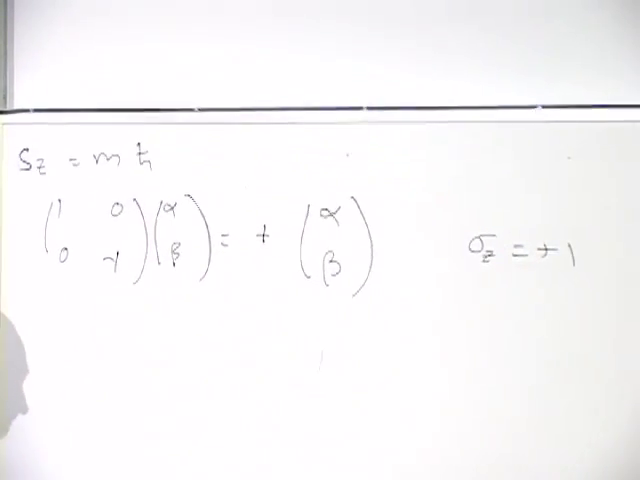
\includegraphics[width=0.74\textwidth]{lecture_08_figure_02.png}\caption{\(+1\) 고유값에 대한 \(\sigma_z\)의 고유값 방정식을 2성분 스피너에 작용시킨 결과.}\lectureframe{00:34:57}\end{figure}

고윳값이 \(+1\)인 경우, 행별로 곱하면 다음을 얻는다.
\begin{equation}
\begin{pmatrix}
1\cdot\alpha+0\cdot\beta\\
0\cdot\alpha-\beta
\end{pmatrix}
=
\begin{pmatrix}
\alpha\\
-\beta
\end{pmatrix}
=
\begin{pmatrix}
\alpha\\
\beta
\end{pmatrix}.
\end{equation}
윗줄 방정식은 자동으로 만족되고, 아랫줄에서 \(-\beta=\beta\)가 나오므로 \(\beta=0\)이다. 정규화 조건은 \(|\alpha|=1\)이다. 중요하지 않은 전체 위상을 \(\alpha=1\)가 되도록 택하면,
\begin{equation}
|+z\rangle=
\begin{pmatrix}
1\\
0
\end{pmatrix}.
\end{equation}

고윳값이 \(-1\)인 경우에는,
\begin{equation}
\begin{pmatrix}
\alpha\\
-\beta
\end{pmatrix}
=
\begin{pmatrix}
-\alpha\\
-\beta
\end{pmatrix}.
\end{equation}
이번에는 아랫줄 방정식이 자동으로 만족되고, 윗줄에서 \(\alpha=-\alpha\)가 나오므로 \(\alpha=0\)이다. \(\beta=1\)로 택하면 다음을 얻는다.
\begin{equation}
|-z\rangle=
\begin{pmatrix}
0\\
1
\end{pmatrix}.
\end{equation}

이제 실험을 바꾸어 \(S_x\)를 측정하자. 다음 관계로부터
\begin{equation}
\sigma_x
\begin{pmatrix}
\alpha\\
\beta
\end{pmatrix}
=
\begin{pmatrix}
0\cdot\alpha+\beta\\
\alpha+0\cdot\beta
\end{pmatrix}
=
\begin{pmatrix}
\beta\\
\alpha
\end{pmatrix},
\end{equation}
\(+1\) 고윳값 방정식은 다음과 같이 된다.
\begin{equation}
\begin{pmatrix}
\beta\\
\alpha
\end{pmatrix}
=
\begin{pmatrix}
\alpha\\
\beta
\end{pmatrix}.
\end{equation}
두 성분 방정식 \(\beta=\alpha\)과 \(\alpha=\beta\)은 같은 조건이다. 정규화하면
\begin{equation}
2|\alpha|^2=1,
\end{equation}
따라서 다음과 같이 택하면 편리하다.
\begin{equation}
|+x\rangle
=
\frac{1}{\sqrt2}
\begin{pmatrix}
1\\
1
\end{pmatrix}.
\end{equation}

\begin{figure}[t]\centering
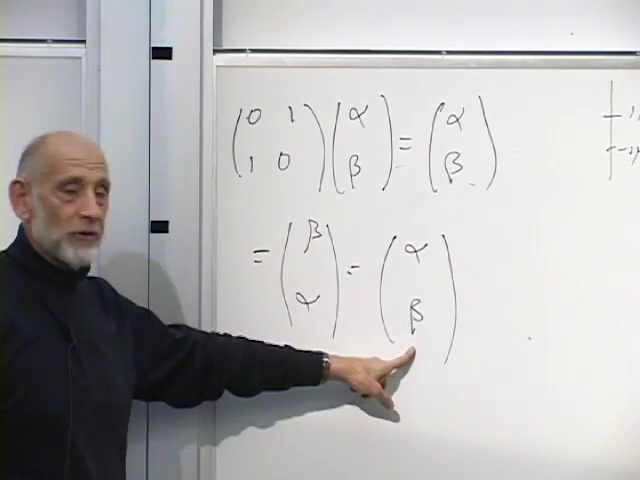
\includegraphics[width=0.74\textwidth]{lecture_08_figure_03.png}\caption{\(+1\) 고유값에서는 \(\sigma_x\)가 두 성분을 서로 바꾸므로 \(\alpha=\beta\)이어야 한다.}\lectureframe{00:39:42}\end{figure}

\begin{classroomqa}
\lecturetimestamp{00:40:13}
\audiencequestion{1/2 인자를 포함하면 고유값도 1/2이 되는가?}
\lecturerresponse{그렇다. 파울리 행렬 \(\sigma_x\)의 고유값은 \(\pm1\)이고, \(S_x=\sigma_x/2\)의 고유값은 \(\pm\tfrac12\)이다.}
\end{classroomqa}

고윳값이 \(-1\)인 경우에는,
\begin{equation}
\begin{pmatrix}
\beta\\
\alpha
\end{pmatrix}
=
-
\begin{pmatrix}
\alpha\\
\beta
\end{pmatrix},
\end{equation}
따라서
\begin{equation}
\beta=-\alpha,
\qquad
\alpha=-\beta.
\end{equation}
이 두 식은 다시 같은 방정식이다. 정규화하면
\begin{equation}
|-x\rangle
=
\frac{1}{\sqrt2}
\begin{pmatrix}
1\\
-1
\end{pmatrix}.
\end{equation}
그러므로 \(z\) 방향 스핀 업 상태와 \(z\) 방향 스핀 다운 상태를 같은 크기로 중첩하면 양의 \(x\)축 방향으로 편극되고, 상대 부호만 마이너스로 바꾸면 음의 \(x\)축 방향으로 편극된다.

\(y\) 방향의 경우,
\begin{equation}
\sigma_y
\begin{pmatrix}
\alpha\\
\beta
\end{pmatrix}
=
\begin{pmatrix}
-i\beta\\
i\alpha
\end{pmatrix}.
\end{equation}
정규화된 두 고유벡터는 다음과 같다.
\begin{equation}
|+y\rangle
=
\frac{1}{\sqrt2}
\begin{pmatrix}
1\\
i
\end{pmatrix},
\qquad
|-y\rangle
=
\frac{1}{\sqrt2}
\begin{pmatrix}
1\\
-i
\end{pmatrix},
\end{equation}
전체 위상은 임의로 정할 수 있다. 두 상태 모두 \(z\) 방향 스핀 업일 확률은 \(1/2\)이고, \(z\) 방향 스핀 다운일 확률은 \(1/2\)이다. 이 두 확률로는 알 수 없는 상대 위상 \(i\)이 \(y\) 편극과 \(x\) 편극을 구별한다. 선형 결합으로 임의의 방향으로 편극된 스핀도 나타낼 수 있지만, 그 계산은 뒤로 미룬다.

\begin{classroomqa}
\lecturetimestamp{00:44:22}
\audiencequestion{\(i\) 성분의 부호가 잘못된 \(\sigma_y\) 고유값에 배정되었는가?}
\lecturerresponse{실제로 그 부호가 잘못된 고유값에 배정되었을 수 있다. 여기서는 어느 쪽에 배정되는지 확실하지 않으며, 기억에 의존해 정하지 않는다.}
\end{classroomqa}

직접 확인하면 다음과 같다.
\begin{align}
\sigma_y\frac{1}{\sqrt2}
\begin{pmatrix}
1\\
i
\end{pmatrix}
&=
\frac{1}{\sqrt2}
\begin{pmatrix}
-i\,i\\
i
\end{pmatrix}
=
\frac{1}{\sqrt2}
\begin{pmatrix}
1\\
i
\end{pmatrix},\\
\sigma_y\frac{1}{\sqrt2}
\begin{pmatrix}
1\\
-i
\end{pmatrix}
&=
\frac{1}{\sqrt2}
\begin{pmatrix}
(-i)(-i)\\
i
\end{pmatrix}
=
-\frac{1}{\sqrt2}
\begin{pmatrix}
1\\
-i
\end{pmatrix}.
\end{align}
따라서 \(+i\)는 고유값 \(+1\)에 속하고, \(-i\)는 고유값 \(-1\)에 속한다.\footnote{말로 제시된 배정은 여러 차례 번복된 뒤에도 확정되지 않았다. 여기 표시한 부호는 행렬을 직접 곱한 결과로 정해진다.} 임의의 방향으로 편극된 상태를 포함해 모든 스핀 1/2 상태는 \(|+z\rangle\)와 \(|-z\rangle\)의 선형결합이다.

\section{스핀 1과 위치 의존 스피너}

스핀 \(1\)에서 가능한 \(S_z\) 값은 \(+1,0,-1\)이다. 따라서 상태 공간은 3차원이다. 스핀 \(1\)은 정수 스핀이며 보손 통계에 해당한다. 같은 각운동량 교환 관계를 만족하는 세 개의 \(3\times3\) 행렬을 구하자.

세 좌표 방향을 대칭적으로 다루는 표현을 아래에 제시한다.\footnote{\(S_y\)의 부호는 \(00{:}48{:}50\) 부근에 보이는 행렬에 따르며, \([S_x,S_y]=iS_z\)에 의해서도 정해진다. 그 부호를 뒤집으면 필요한 교환자의 부호도 반대로 바뀐다.}
\begin{equation}
\begin{aligned}
S_x
&=
i
\begin{pmatrix}
0&0&0\\
0&0&1\\
0&-1&0
\end{pmatrix},
&
S_y
&=
i
\begin{pmatrix}
0&0&1\\
0&0&0\\
-1&0&0
\end{pmatrix},\\
S_z
&=
i
\begin{pmatrix}
0&1&0\\
-1&0&0\\
0&0&0
\end{pmatrix}.
\end{aligned}
\end{equation}
각 행렬은 실수 반대칭 행렬에 \(i\)를 곱한 것이다. 각 행렬에는 \(1\) 하나와 \(-1\) 하나가 있으며, 해당 좌표에 대응하는 행과 열은 0이다. 첫 번째 행렬은 \(S_x\), 두 번째 행렬은 \(S_y\), 세 번째 행렬은 \(S_z\)에 대응한다. 이는 유용한 기억법이다. 이 표현에서 \(S_z\)는 대각행렬이 아니다.

다음과 같이 두자.
\begin{equation}
v=
\begin{pmatrix}
\alpha\\
\beta\\
\gamma
\end{pmatrix}.
\end{equation}
그러면
\begin{equation}
S_zv
=
\begin{pmatrix}
i\beta\\
-i\alpha\\
0
\end{pmatrix}.
\end{equation}
고윳값이 \(+1\)인 경우,
\begin{equation}
i\beta=\alpha,
\qquad
-i\alpha=\beta,
\qquad
0=\gamma.
\end{equation}
따라서 \(\beta=-i\alpha\)이고 \(\gamma=0\)이다. 정규화 조건에서 \(2|\alpha|^2=1\)이므로,
\begin{equation}
|m=+1\rangle
=
\frac{1}{\sqrt2}
\begin{pmatrix}
1\\
-i\\
0
\end{pmatrix}.
\end{equation}
고윳값이 \(-1\)인 경우에는,
\begin{equation}
i\beta=-\alpha,
\qquad
-i\alpha=-\beta,
\qquad
0=-\gamma,
\end{equation}
따라서 \(\beta=i\alpha\), \(\gamma=0\)이고,
\begin{equation}
|m=-1\rangle
=
\frac{1}{\sqrt2}
\begin{pmatrix}
1\\
i\\
0
\end{pmatrix}.
\end{equation}
마지막으로 고윳값이 0인 방정식은 \(\alpha=\beta=0\)을 주므로 \(\gamma\)은 임의로 정할 수 있다. 이를 정규화한 해는 다음과 같다.
\begin{equation}
|m=0\rangle
=
\begin{pmatrix}
0\\
0\\
1
\end{pmatrix}.
\end{equation}
세 고유벡터가 3차원 공간 전체를 이루므로 더 이상의 고윳값은 없다. 계수 \(1/\sqrt2\)는 장식이 아니다. 나중에 이 대수를 아이소스핀에 적용하면 같은 계수가 정량적인 실험 예측에 들어간다.

\begin{classroomqa}
\lecturetimestamp{00:54:10}
\audiencequestion{스핀 1 고유벡터의 복소 성분은 어떻게 읽어야 하는가?}
\lecturerresponse{\(m=+1\)의 성분은 \(1/\sqrt2,-i/\sqrt2,0\)이고, \(m=-1\)의 성분은 \(1/\sqrt2,i/\sqrt2,0\)이며, \(m=0\)의 성분은 \(0,0,1\)이다.}
\end{classroomqa}

다른 세 행렬 조합도 같은 대수를 만족하며 물리적으로 동등하다. 위의 대칭 표현은 세 방향을 똑같이 다루므로 유용하며, 뒤에서도 다시 사용한다.

\subsection{위치 자유도 되살리기}

이제 입자의 운동을 다시 고려하자. 스핀은 위치 및 운동량과 각각 교환하므로, 스핀 성분과 위치 또는 운동량을 함께 지정할 수 있다. 위치와 운동량은 서로 교환하지 않으며, 스핀 성분들도 서로 교환하지 않는다.

움직이는 스핀 1/2 입자는 위치에 따라 달라지는 스피너로 기술된다.
\begin{equation}
\psi(x)=
\begin{pmatrix}
\psi_\uparrow(x)\\
\psi_\downarrow(x)
\end{pmatrix}.
\end{equation}
다음 양들은
\begin{equation}
\rho_{\uparrow_z}(x)=|\psi_\uparrow(x)|^2,
\qquad
\rho_{\downarrow_z}(x)=|\psi_\downarrow(x)|^2
\end{equation}
위치와 스핀에 대한 결합 확률밀도다. 이들을 더하면
\begin{equation}
\rho(x)=\psi^\dagger(x)\psi(x)
=|\psi_\uparrow(x)|^2+|\psi_\downarrow(x)|^2,
\end{equation}
위치 확률밀도가 된다. 입자가 \(x\)에서 검출되었다고 알려진 경우 조건부 확률은 다음과 같다.
\begin{equation}
P(\uparrow_z\mid x)
=
\frac{|\psi_\uparrow(x)|^2}{\psi^\dagger(x)\psi(x)},
\qquad
P(\downarrow_z\mid x)
=
\frac{|\psi_\downarrow(x)|^2}{\psi^\dagger(x)\psi(x)},
\end{equation}
\(\rho(x)\neq0\)일 때 성립한다. 따라서 전자는 공간에 따라 국소 스핀 진폭이 달라질 수 있는 2성분 공간 파동함수로 표현된다.

움직이는 스핀 1 입자에 대해서는 다음과 같이 쓰자.
\begin{equation}
\phi(x)=
\begin{pmatrix}
\phi_1(x)\\
\phi_2(x)\\
\phi_3(x)
\end{pmatrix}.
\end{equation}
공간의 모든 점에서 세 성분은 앞서 사용한 것과 같은 스핀 공간의 벡터를 이룬다. 스핀 1 입자는 정수 스핀을 가지며 보손이다.

\begin{classroomqa}
\lecturetimestamp{01:00:10}
\audiencequestion{\(\phi_1(x)\) 자체가 스핀 1 결과 \(m=+1\)이 나올 확률인가?}
\lecturerresponse{아니다. 이는 선택한 3성분 기저에서의 진폭이다. 특정 스핀 결과를 얻으려면 해당하는 정규화 고유벡터의 브라를 만들고, 파동함수에 사영한 다음 절댓값 제곱을 취해야 한다.}
\end{classroomqa}

\begin{figure}[t]\centering
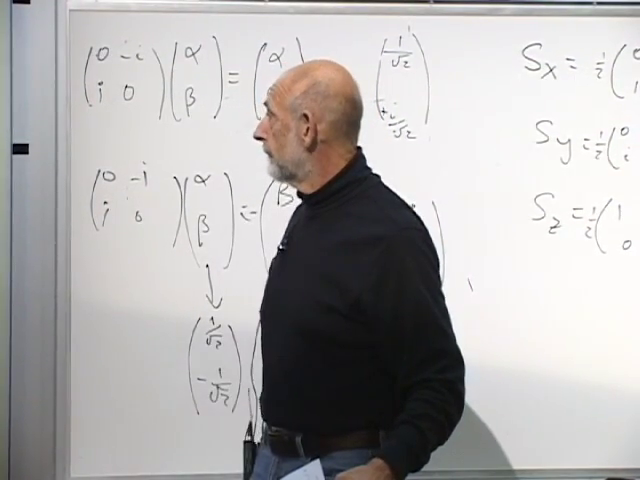
\includegraphics[width=0.82\textwidth]{lecture_08_figure_04.png}\caption{\(\sigma_y\) 정규화 고유벡터와 세 개의 스핀 1/2 행렬.}\lectureframe{01:00:12}\end{figure}

예를 들어,
\begin{equation}
\begin{aligned}
|m=+1\rangle
&=
\frac{1}{\sqrt2}
\begin{pmatrix}
1\\
-i\\
0
\end{pmatrix}
\\
\Longrightarrow\quad\langle m=+1|
&=
\frac{1}{\sqrt2}
\begin{pmatrix}
1&i&0
\end{pmatrix}.
\end{aligned}
\end{equation}
따라서 사영 진폭은
\begin{align}
\langle m=+1|\phi(x)\rangle
&=
\frac{1}{\sqrt2}
\begin{pmatrix}
1&i&0
\end{pmatrix}
\begin{pmatrix}
\phi_1(x)\\
\phi_2(x)\\
\phi_3(x)
\end{pmatrix}\\
&=
\frac{\phi_1(x)+i\phi_2(x)}{\sqrt2}.
\end{align}
같은 규칙을 세 고유벡터 모두에 적용하면 스핀별 밀도를 얻는다.\footnote{이 식들은 \(\phi_1\)와 \(\phi_2\)가 실수일 필요가 없다는 명시적인 정정을 거쳐 사영 대수를 완성한다. 이들을 실수로 취급하면 \(m=+1\) 밀도와 \(m=-1\) 밀도를 구별하는 간섭 효과가 잘못 사라진다.}
\begin{align}
\rho_{+1}(x)
&=
\frac12\left|\phi_1(x)+i\phi_2(x)\right|^2,\\
\rho_{-1}(x)
&=
\frac12\left|\phi_1(x)-i\phi_2(x)\right|^2,\\
\rho_0(x)
&=
|\phi_3(x)|^2.
\end{align}
이들은 다음 관계를 만족한다.
\begin{equation}
\begin{aligned}
\rho_{+1}(x)+\rho_{-1}(x)+\rho_0(x)
&=
|\phi_1(x)|^2+|\phi_2(x)|^2
\\
&\quad{}+|\phi_3(x)|^2
\\
&=
\phi^\dagger(x)\phi(x).
\end{aligned}
\end{equation}
입자가 \(x\)에서 검출되었다고 조건을 걸면,
\begin{equation}
P(m\mid x)
=
\frac{\rho_m(x)}{\phi^\dagger(x)\phi(x)},
\end{equation}
\(\phi^\dagger(x)\phi(x)\neq0\)인 경우에 성립한다. 일반적인 측정 규칙은 늘 같다. 원하는 정규화 고유벡터의 브라를 만들고, 실제 상태를 그 벡터에 사영한 뒤 절댓값을 제곱한다. 이렇게 얻은 밀도에는 위치 의존성이 그대로 남는다.

스핀이 높아지면 행렬은 더 복잡해지지만 원리는 달라지지 않는다.

\begin{classroomqa}
\lecturetimestamp{01:07:31}
\audiencequestion{스핀 3/2의 상태 공간 차원은 얼마인가?}
\lecturerresponse{상태는 네 개이며, \(m=\tfrac32,\tfrac12,-\tfrac12,-\tfrac32\)이다. 스핀 2에는 상태가 다섯 개 있다.}
\end{classroomqa}

\begin{classroomqa}
\lecturetimestamp{01:07:55}
\audiencequestion{\(x,y,z\)는 다루면서 시간 방향은 다루지 않은 이유는 무엇인가? 이 설명은 비상대론적인가?}
\lecturerresponse{지금까지는 비상대론적이다. 질량과 마찬가지로 스핀도 입자의 정지계에서 가장 간단히 특성화할 수 있다. 다른 관성계에서의 기술은 적절한 로런츠 변환으로 얻는다. 이 상대론적 단계는 뒤에서 다룬다.}
\end{classroomqa}

디랙 방정식은 상대론적 틀을 제공하며, 디랙 파동함수가 네 성분을 가지면서 스핀 이중항을 포함하는 이유를 설명한다.

\section{디랙 행렬과 4성분 스피너}

4성분 디랙 파동함수는 다음을 만족한다.
\begin{equation}
i\frac{\partial\Psi}{\partial t}
=
-i\alpha_i\frac{\partial\Psi}{\partial x_i}
+m\beta\Psi,
\qquad i=1,2,3,
\end{equation}
여기서는 반복된 공간 첨자에 대해 합한다. 따라서 미분 항은 다음을 뜻한다.
\begin{equation}
\alpha_1\frac{\partial\Psi}{\partial x}
+\alpha_2\frac{\partial\Psi}{\partial y}
+\alpha_3\frac{\partial\Psi}{\partial z}.
\end{equation}
평면파의 경우 이는 대수 방정식이 된다.
\begin{equation}
\omega\Psi=(\alpha_i k_i+m\beta)\Psi.
\end{equation}

\begin{classroomqa}
\lecturetimestamp{01:11:32}
\audiencequestion{\(m\)가 두 번 나올 때 두 기호는 같은 것을 뜻하는가?}
\lecturerresponse{아니다. 하나는 공간 첨자로 쓰였고, 다른 하나는 입자의 질량이다. 공간 첨자를 \(i\)로 바꾸자. \(i\)가 두 번 나오면 \(1\)부터 \(3\)까지 합한다.}
\end{classroomqa}

진동수 연산자를 제곱하면 상대론적 관계식이 재현되어야 한다.
\begin{equation}
\omega^2=\mathbf{k}^2+m^2.
\end{equation}
따라서 제곱 항으로부터 각 \(i\)에 대해 다음이 요구된다.
\begin{equation}
\alpha_i^2=I_4,
\qquad
\beta^2=I_4.
\end{equation}

\begin{classroomqa}
\lecturetimestamp{01:13:01}
\audiencequestion{\(\beta\)는 \(\Psi\)의 네 성분마다 서로 다른가?}
\lecturerresponse{아니다. 네 성분 스피너 전체에 작용하는 행렬 \(\beta\) 하나가 있으며, 이 행렬은 \(\beta^2=I_4\)를 만족한다.}
\end{classroomqa}

혼합항은 0이어야 한다. 서로 다른 공간 방향 사이뿐 아니라 각 \(\alpha_i\)와 \(\beta\) 사이에서도 다음이 성립한다.
\begin{equation}
\alpha_i\alpha_j+\alpha_j\alpha_i=0
\quad (i\neq j),
\qquad
\alpha_i\beta+\beta\alpha_i=0.
\end{equation}
이를 동등하게 쓰면 다음과 같다.
\begin{equation}
\{\alpha_i,\alpha_j\}=2\delta_{ij}I_4,
\quad
\{\alpha_i,\beta\}=0,
\quad
\{\beta,\beta\}=2I_4.
\end{equation}
각 행렬은 자신과 다른 모든 행렬과 반교환하며, 자기 자신과의 반교환자는 단위행렬의 두 배다.

\(\beta\)를 제외하면 세 파울리 행렬은 이미 항등 행렬로 제곱되고 서로 반교환하는 세 개의 \(2\times2\) 행렬을 제공한다. 질량 항을 위해서는 이 성질을 갖는 네 번째 행렬이 필요하다. 필요한 성질을 만족하는 네 번째 \(2\times2\) 행렬은 없으며, \(3\times3\) 행렬로도 이 대수를 만족시킬 수 없다. 따라서 최소 표현은 \(4\times4\)이다.

\(4\times4\) 행렬은 네 개의 \(2\times2\) 블록으로 나눌 수 있다. 편리한 표현 하나는 다음과 같다.
\begin{equation}
\alpha_i=
\begin{pmatrix}
\sigma_i&0\\
0&-\sigma_i
\end{pmatrix},
\qquad i=1,2,3.
\end{equation}

\begin{figure}[t]\centering
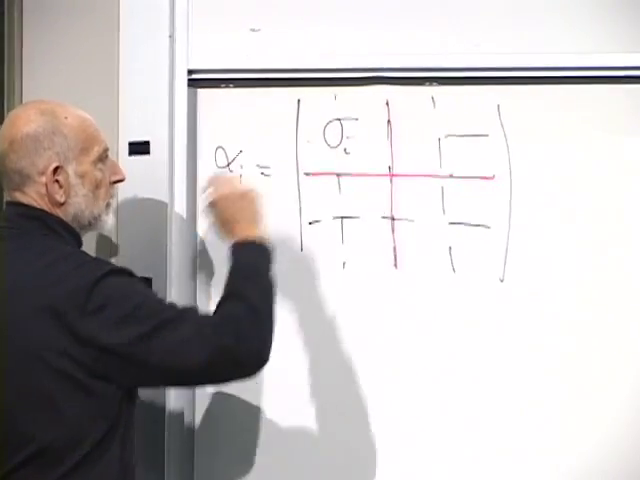
\includegraphics[width=0.68\textwidth]{lecture_08_figure_05.png}\caption{\(\alpha_i\) 디랙 행렬을 \(2\times2\) 블록으로 나타낸 것. 대각 블록은 \(\sigma_i\)와 \(-\sigma_i\)이다.}\lectureframe{01:17:23}\end{figure}

\begin{classroomqa}
\lecturetimestamp{01:17:41}
\audiencequestion{앞선 표현에서는 \(\sigma_i\) 블록이 반대 방식으로 배열되어 있었는가?}
\lecturerresponse{그렇다. 다른 표현에서는 대각선이 아닌 위치에 놓였다. 두 배열은 동등하며 닮음 변환으로 서로 연결된다.}
\end{classroomqa}

현재 표현에서 나머지 행렬은 다음과 같다.
\begin{equation}
\beta=
\begin{pmatrix}
0&I_2\\
I_2&0
\end{pmatrix},
\qquad
I_2=
\begin{pmatrix}
1&0\\
0&1
\end{pmatrix}.
\end{equation}
블록 곱셈을 이용하면 \(4\times4\) 대수의 검산을 보통의 \(2\times2\) 행렬 곱셈으로 줄일 수 있다.

\begin{classroomqa}
\lecturetimestamp{01:19:17}
\audiencequestion{앞선 표현에서 \(\beta\)는 부호가 달랐거나 대각 형태였는가?}
\lecturerresponse{앞선 표현에서는 다르지만 물리적으로 동등한 기저를 사용했다. 기저를 바꾸면 \(\Psi\)의 네 성분이 서로 섞이고 행렬의 모양도 달라지지만, 물리는 변하지 않는다.}
\end{classroomqa}

\(\Psi\)의 네 성분은 시공간의 네 좌표가 아니다. 이 성분들은 반교환 대수가 작용할 수 있는 가장 작은 벡터 공간의 좌표다. 여기에는 서로 다른 두 가지 이중 구조가 있다. \(2\times2\) 블록으로 나뉘고, 각 블록 안에는 2성분 파울리 구조가 있다. 아래에서 확립할 해석을 미리 적용하면 네 가지 경우를 다음과 같이 배열할 수 있다.
\begin{equation}
\begin{array}{c|cc}
& S_z=+\tfrac12 & S_z=-\tfrac12\\ \hline
\omega>0 & (\omega>0,+\tfrac12) & (\omega>0,-\tfrac12)\\
\omega<0 & (\omega<0,+\tfrac12) & (\omega<0,-\tfrac12)
\end{array}.
\end{equation}
아랫줄은 음의 진동수를 갖는 전자 상태들이다. 양전자 행이 아니다. 양전자는 이 상태들의 채워진 집합에 생긴 구멍으로 해석할 것이다.

\section{정지계 에너지 이중성과 양전자}

운동량이 0일 때 에너지의 이중 구조가 가장 쉽게 드러난다. \(\mathbf{k}=0\)이면 평면파 상태는 공간적으로 일정하고 공간 미분 항은 사라진다. 정지계 방정식\footnote{\(01{:}23{:}38\)에서 질량 항에 일시적으로 추가 인자 \(i\)가 붙어 있지만, \(01{:}24{:}05\)에서 구술 중 정정해 이를 제거했다.}은 다음과 같다.
\begin{equation}
i\frac{\partial\Psi}{\partial t}=m\beta\Psi.
\end{equation}

\begin{figure}[t]\centering
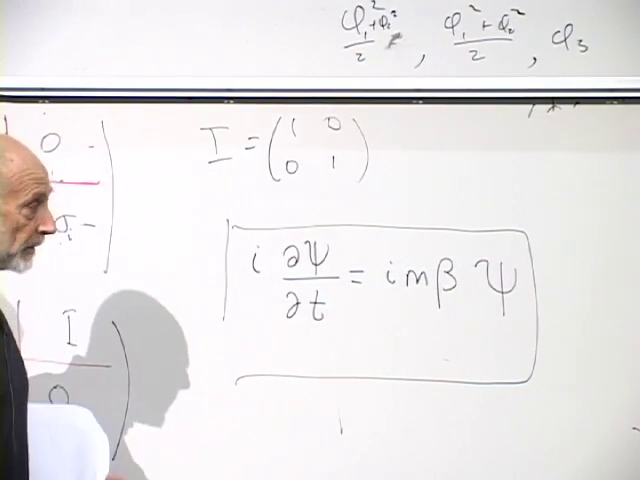
\includegraphics[width=0.76\textwidth]{lecture_08_figure_06.png}\caption{운동량이 0이면 공간 미분항은 사라지고, 보정된 정지계 방정식 \(i\partial_t\Psi=m\beta\Psi\)만 남는다.}\lectureframe{01:23:38}\end{figure}

4성분 열벡터를 위쪽과 아래쪽의 2성분 객체로 나누어 쓰자.
\begin{equation}
\Psi=
\begin{pmatrix}
\psi_+\\
\psi_-
\end{pmatrix}.
\end{equation}

\begin{classroomqa}
\lecturetimestamp{01:24:47}
\audiencequestion{\(\psi_+\)와 \(\psi_-\)라는 표기는 이미 양에너지와 음에너지를 뜻합니까?}
\lecturerresponse{아닙니다. 이 단계에서는 위쪽과 아래쪽의 두 성분 블록을 가리키는 이름일 뿐입니다. 각 블록에 해당하는 에너지 조합은 아직 구하지 않았습니다.}
\end{classroomqa}

\begin{classroomqa}
\lecturetimestamp{01:25:10}
\audiencequestion{나누어 쓴 4성분 열은 무엇을 나타냅니까?}
\lecturerresponse{행렬의 블록 형태에 맞춰 정리한 동일한 4성분 디랙 스피너입니다. 각 절반은 2성분 객체이며, 이런 객체 두 개가 원래의 4성분 열을 이룹니다.}
\end{classroomqa}

행렬 \(\beta\)는 두 블록을 서로 바꿉니다.
\begin{equation}
\beta
\begin{pmatrix}
\psi_+\\
\psi_-
\end{pmatrix}
=
\begin{pmatrix}
\psi_-\\
\psi_+
\end{pmatrix}.
\end{equation}
따라서 정지계 방정식은 다음과 같이 됩니다.
\begin{equation}
i\frac{\partial\psi_+}{\partial t}=m\psi_-,
\qquad
i\frac{\partial\psi_-}{\partial t}=m\psi_+.
\end{equation}

자연스러운 방법은 두 가지입니다. 시간에 대해 한 번 더 미분하면 연립방정식을 분리할 수 있지만, 두 방정식을 더하고 빼면 곧바로 대각화됩니다. 실제로,
\begin{align}
i\frac{\partial}{\partial t}(\psi_++\psi_-)
&=m(\psi_++\psi_-),\\
i\frac{\partial}{\partial t}(\psi_+-\psi_-)
&=-m(\psi_+-\psi_-).
\end{align}
다음과 같이 정의하면
\begin{equation}
\chi_+=\psi_++\psi_-,
\qquad
\chi_-=\psi_+-\psi_-,
\end{equation}
서로 독립인 두 방정식을 얻습니다.
\begin{equation}
i\partial_t\chi_+=m\chi_+,
\qquad
i\partial_t\chi_-=-m\chi_-.
\end{equation}
주파수가 정해진 의존성 \(e^{-i\omega t}\)을 가정하면, 합에 대해서는
\begin{equation}
\omega=+m,
\end{equation}
차에 대해서는
\begin{equation}
\omega=-m.
\end{equation}
를 얻습니다. 이는 앞서 살펴본 1차원 예에서 나타난 양에너지와 음에너지의 이중성과 정확히 같습니다. 상대론적 방정식에는 다시 양에너지 전자 해와 음에너지 전자 해가 존재합니다. 따라서 블록의 이중성은 양에너지 가지와 음에너지 가지로 나뉩니다. 정지계의 순수 상태는 다음과 같이 쓸 수 있습니다.
\begin{equation}
\Psi_{\omega=+m}=
\begin{pmatrix}
\xi\\
\xi
\end{pmatrix},
\qquad
\Psi_{\omega=-m}=
\begin{pmatrix}
\xi\\
-\xi
\end{pmatrix},
\end{equation}
여기서 \(\xi\)는 여전히 임의의 2성분 객체입니다.

합과 차를 취하면 두 겹 구조 가운데 하나는 정리되지만, \(\xi\)의 두 성분은 여전히 남습니다. 파울리 행렬은 이 남은 두 성분에 작용합니다. 이 성분 쌍은 스핀과 관련된 것으로, 아래에서 다룰 회전 및 보존 법칙 검증을 거쳐야 합니다.

\begin{classroomqa}
\lecturetimestamp{01:32:23}
\audiencequestion{스핀을 바깥쪽의 두 겹 구조로, 에너지 부호를 안쪽 구조로 볼 수 있습니까?}
\lecturerresponse{네. 두 인자의 순서는 서로 바꾸어도 동등합니다. 어느 지표를 먼저 쓸지 바꿀 수 있으며, 달라지는 것은 네 성분의 배열뿐입니다.}
\end{classroomqa}

음의 주파수 가지는 디랙 바다 해석으로 이어집니다. 음의 주파수에는 음의 전자 에너지를 대응시킵니다. 배타 원리에 따라 완전한 페르미온 상태 하나에는 전자 하나만 들어갈 수 있으므로, 허용되는 한 모든 음에너지 전자 상태를 채우면 에너지가 낮아집니다. 이렇게 음에너지 상태를 완전히 채운 바다를 진공이라고 부릅니다.

이 채워진 바다에서 전자 하나를 양에너지 상태로 끌어올려 보겠습니다. 그러면 양에너지 전자 하나와 비어 있는 음에너지 상태 하나가 남습니다. 음의 에너지를 제거하면 에너지가 증가하므로, 이 구멍은 양의 여기 에너지를 가집니다. 전자가 하나 빠져 있으므로 전하도 반대 부호입니다. 이 구멍이 양전자입니다.

\begin{classroomqa}
\lecturetimestamp{01:32:57}
\audiencequestion{양전자를 해석하는 방법을 다시 설명해 주시겠습니까?}
\lecturerresponse{두 블록의 합은 양의 주파수를, 차는 음의 주파수를 가집니다. 음의 주파수 해는 음에너지 전자 상태이며, 그 상태를 모두 채우면 진공이 됩니다. 채워진 상태의 전자 하나를 양에너지로 끌어올리면 양에너지 전자와 구멍이 함께 남습니다. 양의 에너지를 가지면서 전하가 반대인 이 구멍이 양전자입니다.}
\end{classroomqa}

따라서 이 대수적 구성에서는 두 가지 결과가 동시에 나옵니다. 양에너지와 음에너지 가지는 입자--반입자 구조로 이어지고, 남은 2성분 구조는 스핀 1/2와 관련됩니다. 놀라운 점은 상대론적 반교환 관계를 만족하는 최소 행렬에서 이 두 결과가 모두 나왔다는 것입니다. 당시 스핀은 실험적으로 알려진 지 얼마 되지 않은 성질이었는데, 이 수학적 구성에서 스핀을 가진 입자와 반입자 가지가 함께 나타났습니다. 당시의 맥락에서 이는 극적인 결과였습니다.

\begin{classroomqa}
\lecturetimestamp{01:35:14}
\audiencequestion{음에너지 전자 자체가 양전자입니까?}
\lecturerresponse{아닙니다. 음에너지 전자 상태는 진공에서 채워져 있습니다. 양전자는 그 채워진 상태들 가운데 전자 하나가 빠진 경우, 즉 구멍이지 음에너지 전자가 아닙니다.}
\end{classroomqa}

구멍은 전이 과정에 참여할 수 있습니다. 양전자가 양의 에너지를 갖는 까닭은 음에너지 전자가 하나 없는 상태이기 때문입니다. 양에너지 전자가 그 구멍을 채우면 전자와 양전자는 소멸하지만, 에너지는 보통 광자의 형태로 빠져나가야 합니다. 바다의 관점에서 보면 전자가 비어 있던 음에너지 상태를 채운 것입니다. 같은 에너지 방출을 원자 안의 여기된 전자가 더 낮은 준위로 내려가는 과정으로 나타낼 수도 있습니다. 아래쪽으로 전이하면서 광자를 방출합니다.

\begin{classroomqa}
\lecturetimestamp{01:36:39}
\audiencequestion{더 높은 음에너지 전자는 왜 구멍으로 떨어지지 않습니까?}
\lecturerresponse{이 질문은 서로 다른 두 경우를 혼동하고 있습니다. 양에너지 전자가 구멍을 채우는 것은 전자--양전자 소멸이며, 광자가 에너지를 가져갑니다. 음에너지 바다의 전자가 전이하는 과정은 다른 과정으로, 아래에서 다룹니다.}
\end{classroomqa}

운동량이 0인 경우의 계산만으로 에너지 부호를 분리한 뒤 두 겹 축퇴가 존재한다는 점은 밝혀졌습니다. 하지만 상태가 두 개라는 축퇴만으로 그 상태들이 각운동량을 가진다고 증명되지는 않습니다.

\begin{classroomqa}
\lecturetimestamp{01:37:44}
\audiencequestion{운동량이 0인 경우의 계산은 남은 상태 쌍이 스핀이라는 것을 어떻게 증명합니까?}
\lecturerresponse{그 상태 쌍을 스핀 위와 아래라고 부를 수 있고 전체 방정식에 파울리 행렬이 나타나지만, 그것만으로는 아직 증명이 되지 않습니다. 이 상태 쌍이 공간 회전 아래에서 어떻게 변환되는지 보이거나, 상호작용과 충돌에서 스핀을 부여했을 때 총각운동량이 보존됨을 보여야 합니다. 그 증명은 뒤에서 다루겠습니다.}
\end{classroomqa}

양에너지를 가진 정지 상태에서는 위쪽 블록과 아래쪽 블록이 같습니다.
\begin{equation}
\Psi_{\omega=+m}=
\begin{pmatrix}
\xi\\
\xi
\end{pmatrix}.
\end{equation}
\(\xi\)가 각운동량 이중항임을 보이려면 앞서 말한 회전 또는 보존 법칙 논증이 필요합니다. 성분이 두 개라는 사실만으로는 이 결론이 나오지 않습니다.

\begin{classroomqa}
\lecturetimestamp{01:40:46}
\audiencequestion{에너지가 서로 달라도 다른 전자가 양전자와 소멸할 수 있습니까?}
\lecturerresponse{네. 전자는 각자 고유한 정체성을 유지하지 않습니다. 가능한 전자라면 어느 것이든 구멍을 채울 수 있으며, 초기 에너지와 운동량의 차이는 방출되는 광자의 수와 에너지에 반영됩니다.}
\end{classroomqa}

구멍의 관점으로 보면 음에너지 바다 안에서만 일어나는 전이도 설명할 수 있습니다. 음에너지 상태 하나에 있던 전자가 구멍으로 이동한다고 합시다. 원래의 구멍은 채워지지만, 전자가 있던 상태가 이제 비게 됩니다. 구멍이 이동한 것입니다. 다시 말해 양전자의 에너지가 바뀌면서 복사를 방출한 것입니다.

\begin{classroomqa}
\lecturetimestamp{01:42:12}
\audiencequestion{인접한 음에너지 준위의 전자들이 왜 차례로 구멍으로 떨어지지 않습니까?}
\lecturerresponse{전자들은 구멍을 한 준위에서 다른 준위로 옮길 수 있습니다. 전자가 기존 구멍으로 내려오면 원래 그 전자가 있던 에너지에 새 구멍이 생기므로, 처음의 양전자는 에너지가 다른 양전자가 됩니다. 에너지 차이는 광자가 가져갑니다.}
\end{classroomqa}

\begin{classroomqa}
\lecturetimestamp{01:44:39}
\audiencequestion{그렇다면 왜 복사를 내며 계속 아래로 내려가는 연쇄 과정이 생기지 않습니까?}
\lecturerresponse{에너지와 운동량이 동시에 보존되어야 하기 때문입니다. 이 두 보존 법칙 때문에 그런 과정이 제한 없이 일어날 수는 없습니다. 보통의 자유 전자도 마찬가지입니다. 빈 공간에서 광자를 방출하며 에너지를 계속 낮출 수는 없습니다.}
\end{classroomqa}

\chapter{라그랑지안, 장, 국소 입자 과정}

보손 장, 페르미온 장, 전자기장은 모두 파동과 같은 방정식을 따릅니다. 이 방정식에는 장 자체와 그 시간 및 공간 미분이 함께 들어갑니다. 각 장마다 운동 방정식을 하나씩 따로 나열할 수도 있지만, 라그랑지안은 전체 계를 하나의 간결한 식으로 모아 줍니다. 그 식에 오일러--라그랑주 규칙을 적용하면 모든 장의 방정식을 한꺼번에 얻습니다.

이 구성은 정지 작용 원리와 밀접하게 관련되어 있습니다. 여기서 당장 할 일은 더 구체적입니다. 장 라그랑지안이 어떤 양에 의존하는지 확인하고, 이를 이용해 몇 가지 고전 방정식을 얻은 다음, 같은 장의 식을 양자역학적으로 다시 해석하는 것입니다. 양자 이론에서 라그랑지안은 입자의 운동과 상호작용을 지배하며, 궁극적으로 충돌의 진폭과 단면적을 결정합니다.

\section{장 방정식을 간결하게 표현하는 방법}

하나의 스칼라 장에 대해 라그랑지안 밀도는 장과 그 1계 미분에 의존합니다.
\begin{equation}
\mathcal L
=
\mathcal L\!\left(\phi,\partial_t\phi,\partial_x\phi,\ldots\right)
=
\mathcal L\!\left(\phi,\partial_\mu\phi\right).
\end{equation}
계산할 때는 시간 및 공간 미분을 명시적으로 나열하는 편이 더 유용할 때가 많습니다. \(\partial_\mu\phi\) 표기는 같은 미분 목록을 상대론적 형태로 묶어 나타냅니다.

\begin{figure}[htbp]
\centering
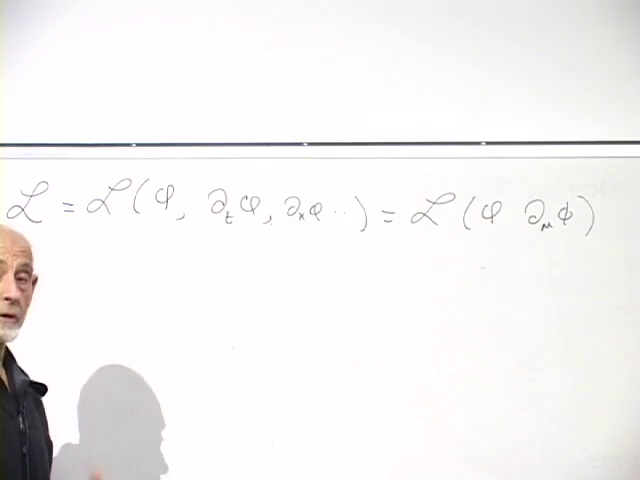
\includegraphics[width=0.82\textwidth]{lecture_09_figure_03.png}
\caption{스칼라 장의 라그랑지안이 장과 시공간 미분에 의존하는 모습.}
\lectureframe{00:03:56}
\end{figure}

장에 대한 오일러--라그랑주 방정식은 다음과 같습니다.
\begin{equation}
\frac{\partial}{\partial t}
\frac{\partial\mathcal L}{\partial\dot\phi}
+
\frac{\partial}{\partial x}
\frac{\partial\mathcal L}{\partial\phi_x}
+
\frac{\partial}{\partial y}
\frac{\partial\mathcal L}{\partial\phi_y}
+
\frac{\partial}{\partial z}
\frac{\partial\mathcal L}{\partial\phi_z}
=
\frac{\partial\mathcal L}{\partial\phi},
\end{equation}
여기서
\begin{equation}
\dot\phi=\frac{\partial\phi}{\partial t},
\qquad
\phi_x=\frac{\partial\phi}{\partial x},
\qquad
\phi_y=\frac{\partial\phi}{\partial y},
\qquad
\phi_z=\frac{\partial\phi}{\partial z}.
\end{equation}
\(\mathcal L\)에 여러 장이 들어 있으면 이 규칙을 각 장에 한 번씩 적용합니다. 그 결과 운동 방정식들의 계를 얻습니다.

가장 간단한 스칼라 예는 다음과 같습니다.
\begin{equation}
\begin{split}
\mathcal L
&=
\frac12\dot\phi^2
-\frac12\phi_x^2
-\frac12\phi_y^2
-\frac12\phi_z^2
-V(\phi)
\\
&=
\frac12\dot\phi^2-\frac12(\boldsymbol\nabla\phi)^2-V(\phi).
\end{split}
\end{equation}
공간 미분 항은 시간 미분 항과 부호가 반대입니다. 각 항을 미분하면
\begin{align}
\frac{\partial\mathcal L}{\partial\dot\phi}&=\dot\phi,
&
\frac{\partial\mathcal L}{\partial\phi_i}&=-\phi_i,
&
\frac{\partial\mathcal L}{\partial\phi}&=-V'(\phi),
\end{align}
따라서
\begin{equation}
\ddot\phi-\nabla^2\phi=-V'(\phi).
\end{equation}

\begin{figure}[htbp]
\centering
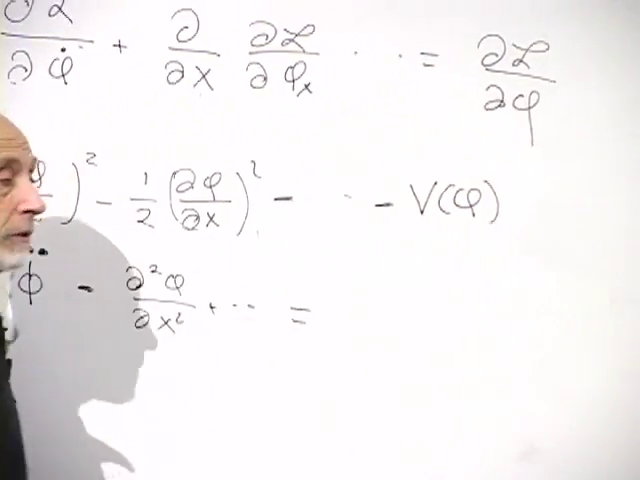
\includegraphics[width=0.74\textwidth]{lecture_09_figure_04.png}
\caption{오일러--라그랑주 방정식, 스칼라 장 라그랑지안, 그리고 \(V(\phi)\)가 만들어 내는 장 방정식.}
\lectureframe{00:08:23}
\end{figure}

이는 스칼라 라그랑지안이 만들어 내는 방정식입니다.\editorialnote{남아 있는 프레임은 왼쪽 가장자리가 잘려 있습니다. 화면에 보이는 완성된 식은 바로 앞뒤의 구술 유도에 따라 정해집니다.}

여기서 \(V(\phi)\)는 장의 퍼텐셜 에너지 밀도이다. \(V\)에 상수항을 더해도 미분하면 사라지므로 이 방정식에는 영향을 주지 않는다. 선형 퍼텐셜도 대수적으로는 가능하지만, 아래쪽 경계가 없다. 즉 장의 에너지는 음의 무한대로 내려갈 수 있다. 따라서 가장 단순한 안정적인 예는
\begin{equation}
V(\phi)=\frac12m^2\phi^2,
\qquad
V'(\phi)=m^2\phi,
\end{equation}
이며, 이로부터 다음을 얻는다.
\begin{equation}
\ddot\phi-\nabla^2\phi=-m^2\phi.
\end{equation}

\(m\)의 의미를 드러내기 위해 평면파를 대입합니다.
\begin{equation}
\phi(\mathbf x,t)=\phi_0e^{i\omega t-i\mathbf k\cdot\mathbf x}.
\end{equation}
그러면
\begin{equation}
\ddot\phi=-\omega^2\phi,
\qquad
\nabla^2\phi=-\mathbf k^2\phi,
\end{equation}
따라서 파동 방정식은 다음과 같이 됩니다.
\begin{equation}
-\omega^2\phi+\mathbf k^2\phi=-m^2\phi.
\end{equation}
\(\phi\)를 약분하면
\begin{equation}
\omega^2=\mathbf k^2+m^2.
\end{equation}
\(\hbar=c=1\)인 단위계에서는 진동수가 에너지이고 파수가 운동량입니다. 따라서
\begin{equation}
E^2=\mathbf p^2+m^2,
\end{equation}
또는 \(c\)의 거듭제곱을 복원하면 \(E^2=\mathbf p^2c^2+m^2c^4\)입니다. 매개변수 \(m\)는 이 장의 양자 하나의 질량입니다.

상대론적 불변성은 간결한 식의 수준에서 부과할 수 있습니다. \(\mathcal L\)가 로런츠 스칼라라면 그 운동 방정식은 로런츠 불변입니다. 시간 미분과 공간 미분 사이의 상대적 부호는 특수 상대론에서 익숙한 시공간 부호입니다.

\section{비선형성과 결합된 고전장}

장에 더 높은 거듭제곱을 포함하면 새로운 종류의 거동이 나타납니다. 만약
\begin{equation}
V(\phi)=\frac12m^2\phi^2+g\phi^3,
\end{equation}
이라면
\begin{equation}
\ddot\phi-\nabla^2\phi=-m^2\phi-3g\phi^2.
\end{equation}
라그랑지안의 이차항은 장에 대해 선형인 방정식을 만듭니다. 삼차항과 그보다 높은 항은 비선형 방정식을 만듭니다.

이 차이는 파동 묶음의 운동에서 드러납니다. 선형 방정식에서는 오른쪽으로 움직이는 파동 묶음과 왼쪽으로 움직이는 파동 묶음을 더해 또 다른 해를 만들 수 있습니다. 두 묶음은 잠시 겹쳐 간섭한 다음 서로 통과해 지나가며 원래 형태로 나타납니다. 비선형 항이 있으면 파동 묶음은 서로에게 영향을 줍니다. 서로 산란하거나 변형되거나 더 복잡한 파동으로 분해될 수 있습니다. 선형파의 일시적인 간섭은 상호작용이 아닙니다. 파동 묶음에 지속적인 변화가 생긴다면 이는 비선형성을 나타냅니다.

두 스칼라 장에서도 같은 양상이 나타납니다. 다음과 같이 두겠습니다.
\begin{align}
\mathcal L
&=
\frac12(\partial_\mu\phi)(\partial^\mu\phi)
+\frac12(\partial_\mu\rho)(\partial^\mu\rho)
-V(\phi,\rho),
\\
V(\phi,\rho)
&=
\frac12m^2\phi^2+\frac12M^2\rho^2+\rho\phi^2.
\end{align}
마지막 항이 없으면 두 방정식은 서로 독립입니다.
\begin{equation}
\ddot\phi-\nabla^2\phi=-m^2\phi,
\qquad
\ddot\rho-\nabla^2\rho=-M^2\rho.
\end{equation}
이 방정식들은 질량이 \(m\)와 \(M\)인 두 종류의 입자 양자를 나타냅니다. 혼합항을 포함하면
\begin{align}
\ddot\phi-\nabla^2\phi&=-m^2\phi-2\rho\phi,
\\
\ddot\rho-\nabla^2\rho&=-M^2\rho-\phi^2.
\end{align}
각 방정식에 이제 다른 장이 들어갑니다. 두 방정식은 결합되어 있고 비선형입니다. \(\phi\) 파동 묶음은 \(\rho\) 파동 묶음을 산란시키며, 그 반대도 마찬가지입니다. 미분항은 에너지--운동량 관계를 결정하고, 미분되지 않은 이차항은 질량을 정하며, 혼합된 고차항은 상호작용을 나타냅니다. 이것이 기본적인 고전적 양상입니다.

\section{디랙 장과 스칼라 결합}

디랙 장의 방정식은 시간에 대해 1계입니다. 세 공간 방향으로 확장할 수 있음을 전제로 1차원 표기로 쓰면 항의 구조는 다음과 같습니다.
\begin{equation}
i\dot\Psi
\simeq
i\alpha\frac{\partial\Psi}{\partial x}+m\beta\Psi,
\qquad
i\boldsymbol\alpha\cdot\boldsymbol\nabla\Psi
=i\sum_i\alpha_i\frac{\partial\Psi}{\partial x_i}.
\end{equation}
행렬 \(\alpha_i\)와 \(\beta\)는 \(\Psi\)의 성분에 작용합니다. 이에 대응하는 라그랑지안에는 \(\partial_t\Psi\)에 선형인 항, \(\alpha_i\)가 포함된 공간 미분 쌍선형항, 그리고 질량 쌍선형항 \(m\Psi^\dagger\beta\Psi\)이 들어갑니다. 여기서는 이 구조적 사실만 알면 충분합니다.\editorialnote{출처에서 시도한 디랙 라그랑지안의 부호, 괄호, 그리고 \(i\)의 위치는 명시적으로 미정으로 남아 있습니다. 이로부터 관례에 따라 달라지는 정확한 식을 추론하지 않습니다.}

\begin{figure}[htbp]
\centering
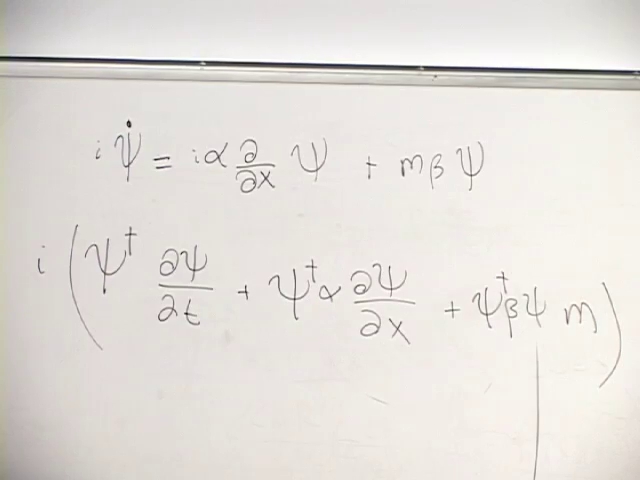
\includegraphics[width=0.76\textwidth]{lecture_09_figure_05.png}
\caption{디랙 장 논의에서의 시간 미분항, 공간 미분항, 질량항.}
\lectureframe{00:25:37}
\end{figure}

\begin{classroomqa}
\lecturetimestamp{00:26:37}
\audiencequestion{시도된 디랙 라그랑지안에서 괄호의 위치는 올바른가요? \(i\)가 전체 식에 곱해지는 건가요?}
\lecturerresponse{여기서는 그 위치를 확신을 가지고 정하지 않으며, 구조적 요점을 위해 꼭 필요한 것도 아닙니다. 디랙 방정식을 만들어 내는 라그랑지안이 존재합니다.}
\end{classroomqa}

이제 스칼라 장 \(\phi\)를 더해 보겠습니다. 단순한 곱 \(\Psi^\dagger\Psi\,\phi\)는 로런츠 스칼라가 아닙니다. 질량항에 나타나는 것과 같은 디랙 행렬을 넣으면
\begin{equation}
\mathcal L_{\mathrm{int}}
\propto
\Psi^\dagger\beta\Psi\,\phi.
\end{equation}
같은 뜻으로 \(\Psi^\dagger\beta\Psi\)는 스칼라 디랙 쌍선형입니다. 전체 라그랑지안을 변분하면 디랙 방정식에는 \(\phi\)에 비례하는 항이 더해지고, 스칼라 방정식에는 \(\Psi^\dagger\beta\Psi\)에 비례하는 원천항이 더해집니다. 두 장은 서로를 산란시킵니다.

\begin{classroomqa}
\lecturetimestamp{00:28:03}
\audiencequestion{스칼라--페르미온 상호작용에 넣은 \(\beta\)는 디랙 질량항에 나타나는 것과 같은 \(\beta\)인가요?}
\lecturerresponse{네. 같은 디랙 행렬입니다.}
\end{classroomqa}

비교식
\begin{equation}
m\Psi^\dagger\beta\Psi
\qquad\hbox{and}\qquad
\Psi^\dagger\beta\Psi\,\phi
\end{equation}
을 보면 결합항에서 질량 매개변수가 스칼라장으로 대체된 것처럼 보인다. 진공 기댓값이 영이 아닌 장을 끝부분에서 살펴볼 때 이 관찰을 다시 다룬다.

지금까지의 해석은 고전적이었습니다. 파동 묶음이 다른 파동 묶음을 산란시킵니다. 장이 연산자가 되면 같은 대수적 구조가 입자에 대해 더 명확한 의미를 갖습니다.

\section{양자장의 거듭제곱이 하는 일}

실수 스칼라 양자장은 생성 연산자와 소멸 연산자를 모두 포함합니다. 개략적으로 쓰면
\begin{equation}
\phi(x)\sim A^+(x)+A^-(x),
\end{equation}
여기서 \(A^+\)는 양자 하나를 생성하고 \(A^-\)는 하나를 소멸시킵니다. 따라서 \(\phi^3(x)\)에는 다음 네 종류의 국소 과정이 들어 있습니다.
\begin{equation}
\phi^3
\sim
(A^+)^3+(A^+)^2A^-+A^+(A^-)^2+(A^-)^3,
\end{equation}
이 개략적 해석에서는 연산자 순서의 세부 사항과 수치 계수를 생략했습니다. 입자 수의 변화는 다음 네 가지입니다.
\begin{equation}
3\longrightarrow0,
\qquad
0\longrightarrow3,
\qquad
2\longrightarrow1,
\qquad
1\longrightarrow2.
\end{equation}
세 장 인자는 모두 같은 점 \(x\)에서 작용합니다. 따라서 하나의 삼차항에는 입자 셋의 소멸, 입자 셋의 생성, 양자 둘이 하나로 합쳐지는 과정, 그리고 양자 하나가 둘로 분리되는 과정이 모두 들어 있습니다. 실제 진폭에서는 에너지--운동량 보존 때문에 이러한 국소적 해석 중 일부가 나중에 제외될 수 있지만, 연산자 곱 자체에는 모두 들어 있습니다.

이차 자유항은 역할이 다릅니다. 먼저 이웃한 점 \(x\)와 \(x'\) 사이의 차이에 붙는 정규화 계수를 잠시 생략하면
\begin{equation}
\partial_x\phi
\ \propto\
\phi(x)-\phi(x').
\end{equation}
제곱하여 전개하면 항의 구조는 다음과 같습니다.
\begin{align}
\frac12(\partial_x\phi)^2
&\ \propto\
\frac12\bigl[\phi(x)-\phi(x')\bigr]^2
\\
&=
\frac12\phi(x)^2
+\frac12\phi(x')^2
-\phi(x)\phi(x').
\end{align}
각 같은 점에서의 제곱에는 여러 연산자 해석이 있습니다. 양자 둘을 생성하거나 둘을 소멸할 수도 있고, 같은 점에서 양자 하나를 소멸시켰다가 다시 생성할 수도 있습니다. 이런 항은 입자를 다른 곳으로 옮기지 않습니다. 교차항은 \(x'\)에서 양자를 소멸시키고 \(x\)에서 생성하거나, 그 반대로 작용할 수 있습니다. 따라서 이 항은 가장 가까운 이웃 사이의 호핑 항으로 작용합니다. 이런 인자가 반복되면 입자가 \(x\)에서 \(x'\)로, 다시 \(x''\)로, 이어서 더 멀리 이동합니다. 이차 미분항은 자유 전파를 지배하고, 삼차항과 그보다 높은 항은 입자를 산란시키고 생성하며 소멸시킵니다.

\begin{classroomqa}
\lecturetimestamp{00:36:07}
\audiencequestion{유한 차분으로 미분을 나타낼 때 점 사이의 거리 \(x-x'\)도 포함해야 하나요?}
\lecturerresponse{그렇습니다. 거리를 \(L\)라고 하면 차분을 제곱한 뒤 인자 \(L^{-2}\)가 생깁니다. 이 수치 인자는 계수를 바꾸지만 호핑이라는 해석은 바꾸지 않습니다.}
\end{classroomqa}

거리를 복원하면
\begin{align}
\frac12(\partial_x\phi)^2
&\longrightarrow
\frac{1}{2L^2}\bigl[\phi(x)-\phi(x')\bigr]^2
\\
&=
\frac{1}{2L^2}\phi(x)^2
+\frac{1}{2L^2}\phi(x')^2
-\frac{1}{L^2}\phi(x)\phi(x').
\end{align}

질량항도 이차항이지만 미분은 포함하지 않습니다.
\begin{equation}
\frac12m^2\phi(x)^2.
\end{equation}
이 항을 입자 하나에 대해 해석하면 들어오는 양자가 같은 점에서 흡수되었다가 다시 방출됩니다. 양자를 이동시키지는 않습니다. 그 점에 양자가 존재하는 정도에 가중치를 주거나, 그런 의미에서 양자의 존재를 세는 항입니다. 같은 연산자 제곱에는 양자 둘을 생성하거나 소멸하는 해석도 포함됩니다. 따라서 운동과 관련해 중요한 차이는 이웃한 점들을 잇는 교차항과 한 점 안에서 작용하는 질량 삽입항 사이에 있습니다.

\section{양자전기역학의 국소 꼭짓점}

이런 기본적인 입자 과정의 개략도에서 파인만 도표가 시작됩니다. 핵심 예는 전자, 양전자, 광자의 이론인 양자전기역학입니다.

디랙 방정식에는 양의 에너지 모드와 음의 에너지 모드가 있습니다. 오래된 표현으로는 \(\Psi\)가 두 종류 모드의 소멸 연산자를 포함하고, \(\Psi^\dagger\)는 이에 대응하는 생성 연산자를 포함합니다. 음의 에너지 전자를 제거하는 것은 양의 에너지를 가진 양전자를 생성하는 것으로 재해석됩니다. 이렇게 표기를 바꾸면 유용한 개략적 분해는 다음과 같습니다.
\begin{align}
\Psi
&\sim
C^-_{e^-}+C^+_{e^+},
\\
\Psi^\dagger
&\sim
C^+_{e^-}+C^-_{e^+}.
\end{align}
따라서 \(\Psi\)는 전자를 소멸시키거나 양전자를 생성하고, \(\Psi^\dagger\)는 전자를 생성하거나 양전자를 소멸시킵니다. 이 약식 표기에는 정규화, 스핀 표지, 운동량 적분이 포함되어 있지 않습니다.

양자전기역학의 상호작용은 디랙 전류와 전자기 벡터 퍼텐셜을 결합합니다. 여기서 사용하는 성분 표기에서 그 구조는 다음과 같습니다.
\begin{equation}
\mathcal L_{\mathrm{QED,int}}
\sim
e\left(
\Psi^\dagger\Psi\,A_0
+
\Psi^\dagger\boldsymbol{\alpha}\Psi\mathbin{\boldsymbol{\cdot}}\mathbf A
\right),
\end{equation}
여기서
\begin{equation}
J^0=\Psi^\dagger\Psi,
\qquad
\mathbf J=\Psi^\dagger\boldsymbol{\alpha}\Psi.
\end{equation}
기호 \(\sim\)가 중요합니다. 시간 성분과 공간 성분 사이의 상대적 부호는 계량 부호 규약과 벡터 퍼텐셜의 규약에 따라 달라집니다. 불변인 진술은 4전류와 4퍼텐셜을 축약한다는 것입니다.\editorialnote{출처는 전류의 시간 성분과 공간 성분을 정하지만, 성분 축약에 적용할 계량 규약은 정하지 않습니다.}

광자장 \(A_\mu\) 자체에는 광자의 생성 및 소멸 연산자가 들어 있습니다. 벡터라는 성질에는 운동량뿐 아니라 광자의 편광---작은 방향 ``표지''도 담겨 있습니다.

\begin{classroomqa}
\lecturetimestamp{00:44:28}
\audiencequestion{\(A_\mu\)가 벡터이고 페르미온 인자는 처음 보면 스칼라 같은데, 상호작용은 어떻게 스칼라가 될 수 있나요?}
\lecturerresponse{페르미온도 4벡터를 제공합니다. \(\Psi^\dagger\Psi\)는 그 시간 성분이고 \(\Psi^\dagger\boldsymbol\alpha\Psi\)는 공간 성분입니다. 이 전류를 \(A_\mu\)와 축약하면 스칼라가 됩니다.}
\end{classroomqa}

\(\Psi^\dagger\), \(\Psi\), \(A_\mu\)의 연산자 내용을 곱하면 하나의 국소 꼭짓점에 대해 익숙한 네 가지 해석을 얻습니다.
\begin{enumerate}\item 전자가 광자를 방출한다;
\item 전자가 광자를 흡수한다;
\item 전자와 양전자가 소멸하여 광자가 된다;
\item 광자가 전자--양전자 쌍을 생성한다.
\end{enumerate}
첫 번째 해석에서 \(\Psi\)는 들어오는 전자를 소멸시키고, \(\Psi^\dagger\)는 나가는 전자를 생성하며, 광자장은 광자를 생성합니다. 광자장의 소멸 부분을 택하면 흡수가 됩니다. 양전자에 해당하는 부분을 택하면 쌍 소멸 또는 쌍 생성이 됩니다. 하나의 국소항에 이 과정들이 모두 들어 있습니다.

페르미온 흐름 도표에서 양전자 선의 화살표는 양전자의 전파 방향과 반대로 향합니다. 이 규약을 따르면 허용된 모든 양자전기역학 꼭짓점에서 페르미온 화살표가 끊기지 않고 이어집니다. 네 가지 해석은 외부 다리를 들어오는 쪽과 나가는 쪽 사이에서 옮겨서 구별할 뿐, 페르미온 흐름선을 끊지는 않습니다.

이 모든 해석에는 같은 계수 \(e\)가 붙습니다. 이는 여기서 사용하는 미시적 규약의 전하입니다. 이 계수는 미세구조상수가 아니라 전하 \(e\)이지만, 두 양은 밀접하게 관련되어 있습니다. 꼭짓점 진폭은 \(e\)에 비례하고, 모든 운동학적 인자와 정규화 인자를 포함하면 그에 대응하는 확률의 척도는 \(e^2\)에 비례합니다.

\begin{classroomqa}
\lecturetimestamp{00:49:44}
\audiencequestion{광자가 전자--양전자로 바뀌는 해석에도 꼭짓점의 다른 해석과 같은 계수가 붙나요?}
\lecturerresponse{네. 같은 전하 계수 \(e\)가 붙습니다.}
\end{classroomqa}

\begin{classroomqa}
\lecturetimestamp{00:49:59}
\audiencequestion{확률에는 단위가 없으니 어떤 스케일링 인자가 있어야 하지 않나요?}
\lecturerresponse{여기서 사용하는 자연스러운 미시적 규약에서 전하 \(e\)는 무차원입니다. 진폭의 척도는 전하이고, 그 제곱이 확률의 척도를 제공합니다.}
\end{classroomqa}

구체적인 그림으로, 전자가 벽에 부딪혀 갑자기 멈추는 상황을 생각해 봅시다. 에너지와 운동량이 광자 형태로 빠져나갈 확률이 있습니다. 그 복사 진폭에 들어가는 기본적인 전자기 인자는 \(e\)이므로 확률의 척도에는 \(e^2\)가 들어갑니다. 이 진술은 결합 인자만 따로 나타낸 것입니다. 실제 확률은 전자의 상태와 운동학에도 달려 있습니다.

\begin{figure}[htbp]
\centering
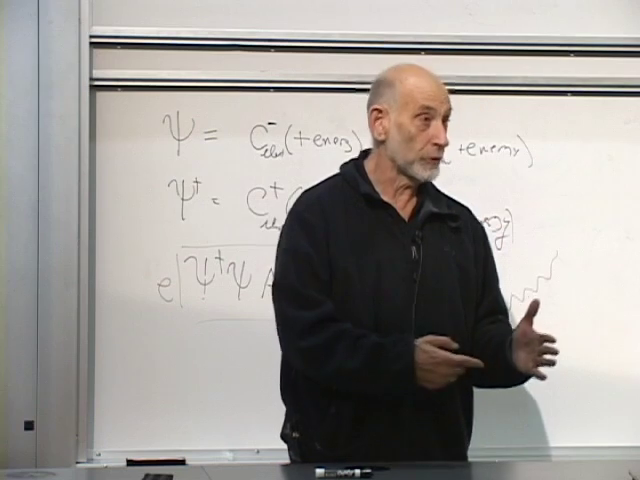
\includegraphics[width=0.78\textwidth]{lecture_09_figure_06.png}
\caption{\(\Psi\)와 \(\Psi^\dagger\)의 전자 및 양전자 연산자 내용과 전자--광자 상호작용 개략도.}
\lectureframe{00:50:39}
\end{figure}

\begin{classroomqa}
\lecturetimestamp{00:51:15}
\audiencequestion{전하에는 단위가 있나요?}
\lecturerresponse{여기서 사용하는 자연스러운 미시적 규약에서는 단위가 없습니다. 거시적 전하는 흔히 쿨롱으로 나타내지만, 입자 이론에서는 전하를 정해 둔 기본 단위를 기준으로 측정합니다. 플랑크 단위나 다른 자연 단위계에서는 물리량을 순수한 수로 나타냅니다.}
\end{classroomqa}

관례와 척도의 차이입니다. 전선의 전류를 다룰 때는 쿨롱이 편리하고, 미시적 진폭을 다룰 때는 무차원 결합이 편리합니다.\editorialnote{00에서 52:37--00:53:15에 나온 ``전하를 가진 항의 묶기''에 관한 짧은 질문은 상당 부분 손상되어 있어, 확정적인 구성을 이끌어 내지 못했습니다.}

기본적인 양자전기역학 상호작용에서 세 장은 모두 한 시공간 점에서 평가됩니다. 꼭짓점 자체에는 내부 시간 지연이 부여되지 않습니다.

\begin{classroomqa}
\lecturetimestamp{00:53:19}
\audiencequestion{전자의 흡수와 재방출, 그리고 광자의 방출은 동시에 일어나나요? 아니면 방정식에 지연이 들어 있나요?}
\lecturerresponse{기본 꼭짓점에서는 모든 연산자가 같은 시공간 점에서 평가됩니다. 따라서 기본 과정에서 이 작용들 사이에는 지연이 없습니다.}
\end{classroomqa}

\begin{classroomqa}
\lecturetimestamp{00:53:57}
\audiencequestion{보존되는 각 물리량은 서로 따로 보존되어야 하나요?}
\lecturerresponse{그렇습니다. 전하는 따로 보존되어야 하는 물리량 가운데 하나입니다.}
\end{classroomqa}

전하 보존은 도표와 대수 양쪽에서 확인할 수 있습니다. 들어오는 전자가 나가는 양전자로 바뀌는 과정은 전하의 부호를 뒤집으므로 허용되는 양자전기역학 꼭짓점이 아닙니다. 시간을 위쪽으로 그리면 전자의 화살표는 시간 방향을 따라 위로 향하고 양전자의 화살표는 아래로 향합니다. 유효한 꼭짓점에서는 페르미온 화살표가 항상 이어집니다. 대수적으로 상호작용에는 \(\Psi\) 하나와 \(\Psi^\dagger\) 하나가 들어 있습니다. 첫 번째 연산자는 전자를 소멸시키거나 양전자를 생성할 때 전하를 한 단위만큼 높이고, 두 번째 연산자는 전하를 한 단위만큼 낮춥니다. 두 효과는 서로 상쇄됩니다.

\begin{classroomqa}
\lecturetimestamp{00:56:05}
\audiencequestion{상자 안의 전자--광자 식이 양자전기역학 라그랑지안 전체인가요?}
\lecturerresponse{아닙니다. 이것은 상호작용항입니다. 전파를 지배하는 이차 자유 광자항과 이차 디랙항은 쓰지 않았습니다.}
\end{classroomqa}

\begin{classroomqa}
\lecturetimestamp{00:56:35}
\audiencequestion{고전 라그랑지안은 유도하고 양자 라그랑지안은 추측한 뒤 검증하나요? 그리고 운동에너지에서 퍼텐셜 에너지를 뺀 구조는 양자역학에서도 유지되나요?}
\lecturerresponse{운동에너지에서 퍼텐셜 에너지를 빼는 양상은 유지됩니다. 시간 미분은 운동에너지 형태를 제공하고, 공간 기울기는 이를 일반화하며, 미분되지 않은 장 항은 퍼텐셜 에너지 형태를 제공합니다. 양자 라그랑지안이 더 근본적인 기술입니다. 양자가 매우 많이 들어 있는 상태에서는 같은 라그랑지안이 고전적인 파동 방정식을 만들어 냅니다. 후보 라그랑지안은 물리 원리와 더 깊은 이론을 바탕으로 제안한 뒤 충돌 실험으로 확립하거나 배제합니다.}
\end{classroomqa}

점유수가 큰 극한은 같은 식이 양자 입자 이론과 그 고전적인 파동을 모두 지배할 수 있는 이유를 설명합니다. 이 일치는 나중에 별도의 기적처럼 덧붙이는 것이 아닙니다. 고전장은 많은 양자가 집단적으로 보이는 거동입니다. 반대로 충돌 실험에서는 기본 꼭짓점이 직접 드러나므로 양자전기역학과 표준 모형의 상호작용을 매우 정밀하게 결정할 수 있습니다.

\section{교차와 시공간 보존 법칙}

국소 꼭짓점의 다리는 들어오는 위치와 나가는 위치 사이에서 교차해 옮겨질 수 있습니다. 나가는 입자를 들어오는 쪽으로 옮기면 그 입자는 반입자로 재해석되며, 반대도 마찬가지입니다. 이런 의미에서 같은 전자--양전자--광자 연산자는 방출, 흡수, 쌍 소멸, 쌍 생성, 심지어 모두 들어오는 국소 해석까지 나타낼 수 있습니다.

\begin{classroomqa}
\lecturetimestamp{00:59:34}
\audiencequestion{기본 꼭짓점 도표를 회전하면 여전히 유효한 국소 해석인가요?}
\lecturerresponse{그렇습니다. 외부 다리를 들어오는 위치와 나가는 위치 사이에서 옮기면 그에 따라 입자--반입자로 재해석할 수 있습니다.}
\end{classroomqa}

국소 연산자 관점만으로는 물리적 과정이 완전히 기술되지 않는다. 꼭짓점이 생길 수 있는 모든 시공간 지점에 대해 진폭을 적분해야 한다. 시간 적분은 에너지 보존을, 공간 적분은 운동량 보존을 보장한다. 전자와 양전자, 광자가 모두 진공 속으로 사라지는 그림은 형식적인 국소 관점으로는 성립하지만, 이 과정은 에너지와 운동량을 보존할 수 없으므로 적분한 진폭은 영이 된다.

\begin{classroomqa}
\lecturetimestamp{01:00:30}
\audiencequestion{모두 들어오는 그림은 전자, 양전자, 광자가 아무것도 남기지 않고 사라질 수 있다는 뜻인가요?}
\lecturerresponse{이는 국소 연산자의 한 해석이지만, 물리적 진폭에는 꼭짓점 위치에 대한 적분이 포함됩니다. 이 적분들은 에너지와 운동량 보존을 강제하므로 운동학적으로 금지된 이 과정의 진폭은 0입니다.}
\end{classroomqa}

\begin{classroomqa}
\lecturetimestamp{01:01:57}
\audiencequestion{그 반대인 진공에서 전자--양전자--광자가 생성되는 해석도 있나요? 배제되는 과정은 적분 뒤에 사라지나요?}
\lecturerresponse{그 반대의 국소 해석도 들어 있습니다. 공간과 시간에 대한 적분은 보존 법칙에 맞지 않는 모든 과정을 제거합니다.}
\end{classroomqa}

라그랑지안의 미분은 생성 및 소멸 기호 자체를 미분하지 않아도 연산자 전개와 잘 맞습니다. 장의 개략적 형태는 다음과 같습니다.
\begin{equation}
\Psi(x)
\sim
\int d^3k\,
\bigl[
C(\mathbf k)e^{i\mathbf k\cdot\mathbf x-i\omega t}
+\cdots
\bigr].
\end{equation}
연산자 \(C(\mathbf k)\)는 이 시공간 전개의 계수입니다. 미분은 평면파에 작용하여 \(\mathbf k\) 또는 \(\omega\)를 끌어냅니다.

\begin{classroomqa}
\lecturetimestamp{01:02:27}
\audiencequestion{장 전개식을 미분할 때 생성 연산자 자체도 미분하나요?}
\lecturerresponse{아닙니다. 이 전개에서 생성 연산자와 소멸 연산자는 시공간 좌표에 의존하지 않습니다. 미분은 지수 인자에 작용해 운동량과 진동수를 끌어냅니다.}
\end{classroomqa}

\section{유효 이론으로서의 핵자와 파이온}

같은 표현법으로 양성자, 중성자, 파이온을 기술할 수 있습니다. 양성자와 중성자는 \(\Psi_p\)와 \(\Psi_n\)라는 장으로 나타내는 페르미온입니다. 상호작용을 세는 이 논의에서는 파이온 장을 세 가지 전하 상태를 갖는 스칼라 장으로 취급합니다.
\begin{equation}
\pi^+,
\qquad
\pi^-,
\qquad
\pi^0.
\end{equation}
양성자와 \(\pi^+\)는 전하를 한 단위만큼 띠고, \(\pi^-\)는 음전하를 한 단위만큼 띠며, 중성자와 \(\pi^0\)는 중성입니다. 더 깊은 수준에서 파이온은 쿼크--반쿼크 계이지만, 처음에는 그 내부 구조를 미정으로 두어도 됩니다.

전하를 보존하는 핵자--파이온 장 곱의 개략적인 목록은 다음과 같습니다.
\begin{equation}
\mathcal L_{N\pi}
\sim
\left\{
\Psi_p^\dagger\Psi_n\,\pi^+,\;
\Psi_n^\dagger\Psi_p\,\pi^-,\;
\Psi_p^\dagger\Psi_p\,\pi^0,\;
\Psi_n^\dagger\Psi_n\,\pi^0
\right\}.
\end{equation}
여기서는 장의 구성과 전하 배정만 나타냅니다. 상대 계수와 부호, 스피너 행렬 구조는 정해져 있지 않습니다. 첫 번째 파이온 장의 전하는 구체적인 해석을 따져 확인할 수 있습니다. 중성자와 양전하 파이온 하나는 양성자를 만들 수 있지만, 그 자리에 음전하 파이온을 쓰면 들어오는 음전하가 나가는 양전하로 바뀝니다. 켤레항은 반대 전하를 띤 과정을 나타냅니다.\editorialnote{출처에서는 전하를 보존하는 한 쌍의 항에 도달하기 전까지 파이온 부호를 여러 차례 수정합니다. 표시된 순서는 최종적인 개략 구조를 반영합니다.}

각 항은 다시 여러 방식으로 교차 해석할 수 있습니다. 나가는 중성자를 들어오는 쪽으로 옮기면 들어오는 반중성자로 바뀝니다. 따라서 전하를 띤 꼭짓점은 양성자와 반중성자가 결합해 \(\pi^+\)가 되는 과정을 나타낼 수 있고, 운동학적으로 가능하면 \(p\to n+\pi^+\) 같은 과정도 나타낼 수 있습니다. 중성 항은 양성자나 중성자가 \(\pi^0\)를 방출하거나 흡수하도록 합니다. 전하 보존은 허용되는 과정의 종류를 정하고, 에너지와 운동량 및 그 밖의 대칭성은 특정 실험에서 그중 어떤 과정이 일어날 수 있는지를 결정합니다.

쿼크 내부 구조가 알려지기 전에는 이것이 유용한 유효 기술이었습니다. 탐침으로 그 구조를 분해해 볼 수 없을 때는 지금도 유용합니다. 양성자에는 원자에 내부 구조가 있는 것처럼 유한한 분포를 가진 구성 입자들이 있지만, 그 규모는 훨씬 작습니다. 실험에서 전달하는 운동량이 양성자를 분해하거나 그 구조를 알아볼 만큼 크지 않다면 양성자를 고유한 장을 가진 점입자로 취급할 수 있습니다. 충분히 높은 에너지의 충돌은 쿼크를 드러내므로, 그때는 점입자로서의 양성자 장만으로는 더 이상 충분하지 않습니다.

양성자는 전하를 띠므로 국소적인 양성자--광자 상호작용도 있습니다. 개략적으로는 \(J_p^\mu A_\mu\)이며, 여기서 \(J_p^\mu\)는 양성자 전류입니다. 전자에도 이에 대응하는 전자--광자 상호작용이 있습니다. 양성자는 광자를 방출하면서 중성자로 바뀔 수는 없습니다. \(p\to n+\gamma\)는 전하 보존을 위반합니다.

\begin{classroomqa}
\lecturetimestamp{01:10:28}
\audiencequestion{양성자와 전자가 상호작용하면 어떻게 되나요?}
\lecturerresponse{각 전하 입자에는 광자 꼭짓점이 있습니다. 양성자는 양성자로 남은 채 광자를 방출할 수 있고, 전자는 전자로 남은 채 그 광자를 흡수할 수 있습니다. 양성자--전자 산란은 이 두 국소 꼭짓점과 그 사이에서 전파되는 광자로 이루어집니다.}
\end{classroomqa}

\section{국소성과 기본 과정의 반복}

양성자--전자 사이의 전체 교환을 나타내는 특별한 비국소 항은 없습니다. 하나의 국소 꼭짓점에서 양성자가 광자를 방출하고, 이차 광자항들이 이웃한 점에서 다음 이웃한 점으로 광자를 전달하며, 또 다른 국소 꼭짓점에서 전자가 이를 흡수합니다. 확장된 과정은 이러한 기본 조각들을 곱해 얻습니다.
\begin{equation}
\begin{aligned}
\bigl[J_p^\mu A_\mu\bigr](x_p)
&\longrightarrow
\underbrace{x_p\to x_1\to x_2\to\cdots\to x_e}_{\text{quadratic photon propagation}}
\\
&\longrightarrow
\bigl[J_e^\nu A_\nu\bigr](x_e).
\end{aligned}
\end{equation}
이 개략적인 연쇄의 화살표는 연이어 일어나는 이웃 점 삽입을 나타내며, 새로운 비국소 상호작용을 뜻하지 않습니다.

\begin{classroomqa}
\lecturetimestamp{01:12:06}
\audiencequestion{양성자와 전자가 서로 교환되는 전체 과정의 라그랑지안은 어떻게 쓸까요--?}
\lecturerresponse{이렇게 전체에 걸친 사건을 나타내는 항을 따로 더하지는 않습니다. 이 과정은 국소적인 양성자--광자 꼭짓점, 반복되는 이차 전파 항, 국소적인 전자--광자 꼭짓점으로 이루어집니다.}
\end{classroomqa}

국소 구조는 두 가지 형태를 가집니다. 미분되지 않은 상호작용 항은 하나의 시공간 점에서 작용합니다. 유한 차분으로 표현되는 미분 항은 그 점을 이웃한 점과만 연결합니다. 어느 형태도 입자를 유한한 거리에 걸쳐 직접 옮기지 않습니다. 장거리 전파는 무수히 많은 무한소 이동을 모아 이루어지며, 기본적인 원격 작용은 없습니다.

\begin{classroomqa}
\lecturetimestamp{01:14:36}
\audiencequestion{라그랑지안에는 한 점에서만 작용하는 항이 들어 있나요?}
\lecturerresponse{상호작용 항은 한 점에서 작용합니다. 미분 항은 한 점과 무한소만큼 이웃한 점을 연결합니다. 방출, 여러 차례의 이웃한 점 사이 이동, 흡수가 함께 유한한 교환을 만들어 냅니다.}
\end{classroomqa}

\begin{classroomqa}
\lecturetimestamp{01:15:36}
\audiencequestion{확장된 과정의 모든 요소가 들어 있나요? 그리고 이 요소들을 결합한다는 것은 곱한다는 뜻인가요?}
\lecturerresponse{그렇습니다. 기본적인 방출, 이동, 흡수는 각각 라그랑지안에 부호화되어 있습니다. 반복 삽입의 곱이 이 요소들을 결합해 더 큰 과정을 이룹니다.}
\end{classroomqa}

여기서 다루는 상대론적 양자장론은 장이 정의되는 시공간을 전제로 합니다. 이를 동역학적 시공간 기하학의 완전한 양자 이론과 혼동해서는 안 됩니다.

\begin{classroomqa}
\lecturetimestamp{01:16:28}
\audiencequestion{블랙홀 사건의 지평선 근처처럼 상대론적 효과가 강한 상황에서도 이런 결합이 유효한가요?}
\lecturerresponse{블랙홀로 확장하는 문제는 이 구성의 범위를 벗어납니다. 여기서 사용하는 양자장론만으로는 중력이 필수적인 블랙홀 동역학을 완전히 기술할 수 없습니다.}
\end{classroomqa}

장은 기본적인 국소 작용을 나타내는 연산자입니다. 장 인자 하나는 입자를 흡수하거나 방출할 수 있습니다. 인자 두 개의 곱은 한 입자를 흡수하고 같은 점에서 다른 입자를 방출할 수 있으며, 더 높은 차수의 곱은 입자 구성을 더 바꿀 수 있습니다. 국소 연산자들의 곱은 이런 작용을 이어 역사로 만듭니다. 시공간에서 운동은 작은 영역에서 흡수하고 이웃한 영역으로 다시 방출한 뒤, 또 흡수하고 다시 방출하는 과정으로 나타냅니다. 걸음의 크기를 0에 가깝게 줄이면서 걸음 수를 늘리면 연속 궤적을 얻습니다.

\begin{classroomqa}
\lecturetimestamp{01:17:30}
\audiencequestion{이 국소적 걸음 그림에서 장, 거리, 시간은 어떻게 이해해야 하나요?}
\lecturerresponse{장은 국소적인 흡수와 방출을 나타내는 연산자입니다. 그 곱은 기본 작용들을 이어 주며, 시공간을 지나는 운동은 연속 극한을 취하기 전에 무한소로 이웃한 점들 사이의 걸음으로 구성됩니다.}
\end{classroomqa}

따라서 정칙화된 출발점은 시공간을 작은 셀들로 나누고, 장 연산자를 각 셀에 붙이는 것입니다.\editorialnote{01:17:30--01:20:40에서 청중의 발언은 일부가 가려져 있습니다. 의역한 질문에는 확인할 수 있는 주제만 담았고, 국소 연산자와 시공간의 연속된 걸음에 관한 답변은 분명합니다.} 미분은 차분이 됩니다. 이차 교차 항은 이웃한 셀들을 연결하고, 질량 항과 상호작용 항은 하나의 셀 안에서 작용합니다. 셀은 극한 이론을 정의하기 위한 장치이지, 추가 입자나 새로운 물리적 질량 척도가 아닙니다.

특수상대론적 효과를 각 단계마다 따로 더할 필요는 없습니다. 라그랑지안이 로런츠 스칼라라면, 그로부터 구성되는 진폭은 로런츠 불변이며 시간 지연 같은 효과도 그 구조에서 따라 나옵니다.

\begin{classroomqa}
\lecturetimestamp{01:21:10}
\audiencequestion{고에너지 운동과 시간 지연은 여러 단계를 거치는 과정에 추가적인 문제를 일으키나요?}
\lecturerresponse{별도의 보정은 필요하지 않습니다. 라그랑지안이 로런츠 스칼라라면 시간 지연 같은 특수상대론적 효과가 이미 결과에 포함되어 있습니다. 다만 질문의 구체적인 우려가 무엇인지는 완전히 분명하지 않습니다.}
\end{classroomqa}

생성 연산자와 소멸 연산자는 위치 기저나 운동량 기저로 나타낼 수 있습니다. 위치 공간의 생성 연산자는 운동량 공간 생성 연산자들의 푸리에 중첩이며, 그 역도 성립합니다. 위치와 운동량이 모두 정확히 정해진 상태를 생성하는 연산자는 없습니다. 입자의 위치를 정밀하게 국소화하려면 넓은 운동량 범위가 필요하고, 운동량을 정밀하게 국소화하면 위치 공간에서 넓게 퍼집니다. 이 언어로 표현한 두 기저 사이의 푸리에 관계가 불확정성 원리입니다.

\begin{classroomqa}
\lecturetimestamp{01:22:48}
\audiencequestion{생성 및 소멸 연산자는 위치, 운동량, 불확정성 원리와 어떻게 관련되나요?}
\lecturerresponse{이 연산자들은 위치의 함수로도, 운동량의 함수로도 나타낼 수 있습니다. 두 표현은 서로 푸리에 변환 관계입니다. 위치를 정밀하게 국소화한 상태에는 여러 운동량이 필요하고, 운동량을 정밀하게 국소화한 상태는 위치 공간에서 퍼져 있습니다. 동시에 정밀하게 정해진 \(x\)와 \(p\)를 생성하는 연산자는 없습니다.}
\end{classroomqa}

이제 셀 구성을 완전히 기술할 수 있습니다. 셀에 \(n\)라는 표지를 붙이고, 미분을 다음과 같은 유한 차분으로 바꿉니다.
\begin{equation}
\partial_\mu\phi(x)
\longrightarrow
\frac{\phi_{n+\hat\mu}-\phi_n}{a},
\end{equation}
각 장 종을 모든 셀에 둡니다. 이차 교차 항은 한 셀에서 양자를 없애고 이웃 셀에서 생성합니다. 정칙화된 식을 정의한 뒤 간격 \(a\)을 0에 가깝게 줄이면 연속 이론을 얻습니다.
\begin{equation}
\underbrace{\phi_n\phi_{n+\hat\mu}}_{\text{hop }n\leftrightarrow n+\hat\mu},
\qquad
\underbrace{m^2\phi_n^2}_{\text{same-cell mass insertion}}.
\end{equation}

\begin{classroomqa}
\lecturetimestamp{01:25:16}
\audiencequestion{시공간을 셀들로 나누는 구성을 완성할 수 있나요?}
\lecturerresponse{그렇습니다. 장에 셀별 표지를 붙이고, 미분을 유한 차분으로 바꾸며, 이차 항으로 입자를 이웃 셀 사이에서 이동시킵니다. 셀의 크기를 0에 가깝게 줄이면 연속체를 얻습니다.}
\end{classroomqa}

전자는 이차 항을 통해 셀 사이를 이동하고, 광자도 마찬가지입니다. 한 셀에서 전자와 광자가 만나면 QED 상호작용이 전자를 흡수했다가 다시 방출하는 동시에 광자를 생성하거나 소멸시킬 수 있습니다. 스칼라 질량 항은 같은 셀 안에서 해석됩니다. 입자가 그 셀에 들어갔다가 나가며, 그 계수는 \(m^2\)에 비례합니다. 이 항은 셀 사이 이동을 일으키지 않습니다.

\begin{classroomqa}
\lecturetimestamp{01:28:18}
\audiencequestion{셀의 크기는 질량 계수와 관련이 있나요?}
\lecturerresponse{아니요. 셀의 크기는 궁극적으로 0에 가깝게 줄이는 정칙화 간격이고, 질량 계수는 라그랑지안의 독립적인 매개변수입니다.}
\end{classroomqa}

\begin{classroomqa}
\lecturetimestamp{01:28:43}
\audiencequestion{국소 인자들을 곱하는 것은 단순한 시간 순서가 아니라 시공간 전체에 걸친 공동 진폭을 구성하는 것인가요?}
\lecturerresponse{그렇습니다. 셀은 시공간을 채우고, 각 셀의 국소 기여가 시공간 격자 전체에 걸쳐 결합됩니다. 이 곱은 필요한 국소 사건과 전파 단계의 공동 진폭을 제공합니다.}
\end{classroomqa}

\section{원천, 검출기, 그리고 그 사이의 동역학}

완전한 과정은 시공간에서의 역사입니다. 초기 조건은 실험자가 준비하는 것으로 정하고, 최종 조건은 검출기에 기록되는 것으로 정합니다. 간단한 원천의 예로 전자를 방출하는 가열 필라멘트가 있습니다. 필라멘트 위치의 장 연산자는 들어오는 전자를 생성하고, 검출기 위치의 장 연산자는 전자가 나중에 흡수되는 과정을 기술합니다.

\begin{classroomqa}
\lecturetimestamp{01:29:30}
\audiencequestion{이런 시공간 과정의 초기 단계는 무엇인가요?}
\lecturerresponse{원천에서 준비합니다. 가열 필라멘트가 전자를 방출하는 것이 간단한 예입니다. 필라멘트 위치의 장 연산자가 전자를 생성하고, 검출기의 장 연산자들은 최종 흡수 사건을 지정합니다.}
\end{classroomqa}

같은 구성을 진공 상태에서 시작해 기술할 수도 있습니다. 원천의 생성 연산자는 진공 위에 들어오는 상태를 만듭니다. 검출기와 연관된 소멸 연산자는 나가는 상태를 선택합니다. 이 연산자들은 경계 조건을 지정하며, 원천과 검출기 사이 영역 전체의 동역학을 대신하지는 않습니다.

\begin{classroomqa}
\lecturetimestamp{01:31:11}
\audiencequestion{계 전체가 아니라 방출기에서만 동역학이 작용한다고 두면 잘못인가요?}
\lecturerresponse{그렇습니다. 진공에서 시작해 원천 연산자로 들어오는 입자를 준비하고 검출기 연산자로 최종 입자를 선택합니다. 그 사이에는 반복되는 라그랑지안 삽입이 시공간 전체에서 작용해 입자를 이동시키고, 생성하고, 소멸시킵니다.}
\end{classroomqa}

삽입이 충분히 많으면 여러 입자가 동시에 많은 이웃 셀을 지나 이동할 수 있고, 그 과정에서 입자가 생성되거나 소멸될 수도 있습니다. 초기 연산자는 무엇이 들어오는지를, 최종 연산자는 무엇이 검출되는지를 나타내며, 반복되는 라그랑지안 작용은 그 사이의 모든 과정을 제공합니다.

\begin{classroomqa}
\lecturetimestamp{01:33:24}
\audiencequestion{라그랑지안 삽입을 임의로 많이 할 수 있다면 삽입 위치를 적분하나요?}
\lecturerresponse{그렇습니다. 삽입의 시공간 위치를 적분합니다. 여기서는 정확한 파인만 규칙을 유도하지 않습니다. 당장은 간단한 국소 장 표현이 완전한 과정을 구성하는 기본 상호작용을 부호화한다는 점이 핵심입니다.}
\end{classroomqa}

\section{위상 대칭, 전하, 진폭}

기본 과정을 라그랑지안으로 쓰면 그 대칭성도 드러납니다. 전자장의 전역 위상 변환을 생각해 봅시다.
\begin{equation}
\Psi\longrightarrow e^{i\theta}\Psi,
\qquad
\Psi^\dagger\longrightarrow e^{-i\theta}\Psi^\dagger,
\qquad
A_\mu\longrightarrow A_\mu.
\end{equation}
\(\Psi\)와 \(\Psi^\dagger\)의 수가 같은 항은 위상이 상쇄되어 변하지 않습니다. 그 수가 서로 다른 항에는 위상이 붙습니다. 두 수가 같다는 조건이 전하 보존의 대수적 표현입니다.

이것이 라그랑지안 기술의 핵심적인 장점입니다. 장 인자는 기본 과정을 드러내고, 그 조합은 대칭성을 드러내며, 대칭성은 보존 법칙을 드러냅니다. 반복 삽입은 준비된 초기 상태를 선택된 최종 상태로 변화시킵니다. 그 결과가 양자 진폭입니다. 정확한 계산에는 파인만 규칙이 필요하지만, 구조적 내용은 이미 드러납니다. 국소 작용은 보존 법칙이 허용하는 모든 차수로 반복됩니다.

\section{장 측정과 교환자}

장 연산자는 보통의 양자역학적 연산자와 같은 의미를 지닙니다. 고윳값은 장을 측정했을 때 가능한 결과이고, 고유벡터는 그 값에 대응하는 상태를 나타냅니다. 전하를 띤 입자를 전기장 안에 놓고 입자가 어떻게 가속되는지 관찰하면 전기장을 탐침할 수 있습니다.

\begin{classroomqa}
\lecturetimestamp{01:37:06}
\audiencequestion{장 연산자의 고윳값과 고유벡터도 보통의 양자역학에서와 같은 역할을 하나요?}
\lecturerresponse{그렇습니다. 고윳값은 측정 가능한 장의 값이며, 입자에 미치는 효과를 통해 장을 탐침할 수 있습니다. 교환자는 동시 측정에 어떤 제약이 있는지 결정합니다.}
\end{classroomqa}

자명한 항등식
\begin{equation}
[\phi(x),\phi(x)]=0
\end{equation}
만으로는 측정에 관한 문제가 해결되지 않습니다. 두 관측량과 그 시공간적 관계를 지정해야 합니다. 장과 그 켤레 운동량은 서로 교환하지 않는 정준 쌍이며, 시간꼴로 떨어진 점의 장 연산자들은 교환하지 않을 수 있습니다. 반면 국소 보손장은 국소성에 따라 공간꼴로 떨어진 점에서 서로 교환합니다. 따라서 교환자와 불확정성의 익숙한 관계는 올바른 연산자 쌍을 식별한 뒤에 적용됩니다.\editorialnote{원문은 서로 다른 점에서의 비가환성을 지나치게 넓게 서술합니다. 여기서는 측정에 관한 요점을 살리면서 공간꼴로 분리된 국소 보손장의 미시적 인과율을 지키도록 한정했습니다.}

\begin{classroomqa}
\lecturetimestamp{01:39:57}
\audiencequestion{전기장 또는 전자기장은 볼트 단위로 측정하나요, 아니면 미터당 볼트 단위로 측정하나요?}
\lecturerresponse{전기장은 미터당 볼트 단위로 측정합니다. 볼트와 미터는 미시적인 장 과정을 설명하기에 가장 유용한 언어가 아닙니다. 그런 과정은 광자라는 개념으로 더 자연스럽게 다룰 수 있습니다. 반대로 집에 물을 주는 방법을 판단할 때 양자장론은 유용한 언어가 아닙니다.}
\end{classroomqa}

한 기술에서 자연스러운 단위가 다른 기술에서도 이해를 돕는 것은 아닙니다. 볼트와 미터당 볼트는 거시적 장치에 적합하고, 광자의 생성과 소멸은 미시적 과정에 적합합니다.

\begin{classroomqa}
\lecturetimestamp{01:41:10}
\audiencequestion{라그랑지안 항을 더 큰 과정으로 결합하는 구성 요소로 보는 것이 핵심인가요?}
\lecturerresponse{그렇습니다. 기본 과정은 한 점에서 다음 점으로 반복됩니다. 각 기본 요소는 한 시공간 점에서 작용하거나 미분 항을 통해 이웃한 점들을 연결합니다. 겉보기에는 비국소적인 전파도 이런 국소적 걸음으로 구성되며, 기본적인 원격 작용은 없습니다.}
\end{classroomqa}

\section{국소 과정의 곱과 경로에 대한 합}

국소 과정의 반복을 간결한 방식으로 나타내는 직관적인 방법이 있습니다. 시공간을 셀로 나누고 다음과 같이 씁니다.
\begin{equation}
\prod_x\bigl(1+\mathcal L_I(x)\bigr),
\end{equation}
여기서 \(x\)은 셀에 붙인 표지이고 \(\mathcal L_I(x)\)은 국소 상호작용 라그랑지안입니다. 이는 정확한 연속체 공식이 아닙니다. 곱을 전개하면 허용된 국소 사건의 선택이 모두 어떻게 생성되는지 보여 주는 조합론적 대용 표현입니다.

\begin{classroomqa}
\lecturetimestamp{01:42:18}
\audiencequestion{생성과 전파, 소멸의 여러 단계를 하나의 식으로 간결하게 나타낼 수 있나요?}
\lecturerresponse{직관적으로는 모든 시공간 셀마다 인자 \(1+\mathcal L_I(x)\) 하나씩을 곱하면 됩니다. 곱을 전개하면 사건이 전혀 없는 항, 선택한 임의의 한 점에서 사건 하나가 일어나는 항, 여러 점에서 사건이 일어나는 항이 생깁니다.}
\end{classroomqa}

셀 두 개에 대해서는
\begin{align}
\bigl(1+\mathcal L_I(x)\bigr)
\bigl(1+\mathcal L_I(x')\bigr)
&=
1+\mathcal L_I(x)+\mathcal L_I(x')
\notag\\
&\quad{}+\mathcal L_I(x)\mathcal L_I(x').
\end{align}
첫 번째 항은 어느 쪽에서도 상호작용이 일어나지 않음을 뜻합니다. 다음 두 항은 각각 \(x\) 또는 \(x'\)에서 기본 상호작용 하나가 일어나는 경우를 나타냅니다. 마지막 항은 두 점 모두에서 상호작용이 일어나는 경우입니다. 인자가 많아지면 한 점, 두 점, 세 점 등에서 사건이 일어나는 항들이 포함됩니다. 꼭짓점이 여러 개인 항은 예를 들어 들어오는 입자 두 개가 나가는 입자 세 개를 만드는 과정을 나타낼 수 있습니다.

이차 전파 항도 같은 구성에 들어갑니다. 유한한 변위는 이웃한 점들에서 삽입이 이어지는 사슬로 나타냅니다. 전개된 곱에는 한 셀, 그 이웃 셀, 다음 이웃 셀 등에서의 인자가 들어 있어 입자를 한쪽 끝에서 다른 쪽 끝으로 전달하는 항들이 포함됩니다.

\begin{classroomqa}
\lecturetimestamp{01:46:29}
\audiencequestion{유한한 전파에 여러 국소 운동 항이 필요하다면 필요한 운동은 어떻게 복원하나요?}
\lecturerresponse{큰 곱에는 이웃한 삽입들이 이어져 입자를 초기 위치에서 최종 위치까지 옮기는 사슬이 들어 있습니다. 대개 여러 경로를 따라 이런 사슬이 여럿 존재합니다. 각 경로는 진폭을 기여하며 전체 진폭은 그 진폭들의 합입니다.}
\end{classroomqa}

\(r\)이 경로를 나타낸다면, 도식적으로
\begin{equation}
\mathcal A_{\mathrm{total}}=\sum_r\mathcal A_r,
\qquad
P=\left|\mathcal A_{\mathrm{total}}\right|^2.
\end{equation}
보통의 확률을 각 경로에 부여한 뒤 더하는 것은 아닙니다. 먼저 진폭을 더합니다.
\begin{equation}
\left|\sum_r\mathcal A_r\right|^2
=
\sum_r|\mathcal A_r|^2
+
\sum_{r\ne s}\mathcal A_r\mathcal A_s^*.
\end{equation}
교차항이 간섭을 나타냅니다.

\begin{classroomqa}
\lecturetimestamp{01:48:27}
\audiencequestion{이중 슬릿 실험과 양립하나요?}
\lecturerresponse{그렇습니다. 두 슬릿을 통과하는 대안적 경로는 각각 진폭을 기여합니다. 그 진폭의 합을 제곱하면 간섭항이 생기며, 국소적 걸음 구성에서 시공간을 지나는 여러 경로가 간섭하는 방식도 이와 같습니다.}
\end{classroomqa}

\begin{classroomqa}
\lecturetimestamp{01:49:00}
\audiencequestion{각 인자 안의 \(1\)은 어디에서 나오나요?\(1+\mathcal L_I\)}
\lecturerresponse{이는 셀이 상호작용이 없는 경우와 상호작용이 있는 경우를 모두 기여할 수 있게 하는 조합론적 장치입니다. 경로 적분 방법과 관련은 있지만, 여기에 보인 곱은 기술적 표현을 직관적으로 근사한 것일 뿐입니다.}
\end{classroomqa}

정확한 형식론은 적절한 시공간 적분, 순서화, 정규화, 위상을 제공합니다. 이 곱은 전체 형식론인 척하지 않으면서 여러 조합을 드러낸다는 점에서 유용합니다.

\begin{classroomqa}
\lecturetimestamp{01:49:57}
\audiencequestion{이것이 정지 작용의 원리인가요?}
\lecturerresponse{아닙니다. 고전적인 정지 작용은 특별한 고전 궤적 하나를 선택합니다. 양자역학에서는 궤적마다 작용이 정하는 가중치를 갖는 진폭을 모두 합합니다. 사무실에서 가까운 집으로 가는 길에 파리를 거치는 극도로 돌아가는 경로---도---}양자 합에 포함됩니다.\end{classroomqa}

관계는 미묘하지만 둘의 차이는 간단합니다. 고전역학은 정지 경로를 선택합니다. 양자역학은 경로들을 합하며, 적절한 극한에서는 고전 궤적 주변에서 위상들이 보강됩니다.

\section{라그랑지안을 추론하고 영역을 선택하기}

라그랑지안과 구체적인 과정이 주어지면 그 확률을 계산하는 규칙은 명확합니다. 어려운 수학 문제와 마찬가지로 계산에는 독창적인 발상이 필요할 수 있지만, 더 근본적인 불확실성은 자연이 어떤 장과 결합을 사용하는지 알아내는 데 있습니다.

\begin{classroomqa}
\lecturetimestamp{01:50:43}
\audiencequestion{라그랑지안을 표현하는 데 묘미가 있나요, 아니면 그것을 활용하는 데 있나요?}
\lecturerresponse{핵심은 실험 자료로부터 라그랑지안을 추론하는 데 있습니다. 라그랑지안을 알고 나면 입자 두 개가 들어와 네 개가 나가는 것과 같은 과정의 진폭은 정밀한 규칙에 따라 계산할 수 있습니다. 수학을 실제로 풀어 나가는 데 재치가 필요할 수는 있지만, 그것은 이론의 모호함이 아닙니다.}
\end{classroomqa}

입자 충돌은 기본 꼭짓점을 드러냅니다. 대칭성과 더 깊은 원리의 지침에 따라 항을 제안하고, 그 항들이 만들어 내는 진폭을 관측 결과와 비교해 검증합니다. 검증에 성공하면 허용되는 장의 조합과 그 수치 계수가 정해집니다.

\begin{classroomqa}
\lecturetimestamp{01:52:24}
\audiencequestion{상호작용마다 라그랑지안이 따로 있나요---아니면 라그랑지안이 한 권 가득인가요?}
\lecturerresponse{실제로는 모든 장과 상호작용을 담은 하나의 큰 라그랑지안으로 보는 것이 작업상의 그림입니다. 다만 궁극적으로 이 그림이 틀릴 수도 있습니다. 그 합의 일부로 알아볼 수 있는 영역들이 나타납니다. 새로운 입자가 추가되면 장이 하나 늘고, 새로운 기본 과정이 추가되면 상호작용 항이 하나 늘어납니다.}
\end{classroomqa}

완전한 식이 어수선할 수는 있어도 책 한 권 분량일 필요는 없습니다. 대략적인 규모를 보이기 위한 거친 예로, 기본 입자라 불리는 대상이 백 개 안팎이고 항이 수백 개라고 생각해 볼 수 있습니다. 양자전기역학, 강한 상호작용과 약한 상호작용, 중력 영역을 합쳐도 빽빽하게 쓴 몇 쪽에 들어갈 수 있습니다. 정확한 개수는 요점이 아닙니다. 작업상의 그림은 알아볼 수 있는 여러 조각을 모아 하나의 동역학적 표현을 만드는 것이며, 이 그림이 언젠가 불완전한 것으로 드러날 수도 있음을 명시하고 있습니다.

장이 더 근본적인 시공간 기하학을 결정하는지 여부는 여기서 사용하는 표준 양자장론의 범위를 벗어납니다.\editorialnote{01:55:00--01:55:20에서 나온 질문은 손상이 심해 다양체나 기하학적 구성을 신뢰성 있게 알아볼 수 없습니다. 범위의 한계에 관한 답변만 확실합니다.}

\begin{classroomqa}
\lecturetimestamp{01:55:22}
\audiencequestion{실험으로 결정되는 수치가 결합 상수인가요?}
\lecturerresponse{결합 상수는 라그랑지안 항의 계수입니다. 이차 질량 항의 계수 \(m^2\)가 한 예이며, \(\phi^4\)이나 \(\phi^6\) 또는 그보다 높은 거듭제곱 항의 계수도 마찬가지입니다.}
\end{classroomqa}

각 장 곱에는 생성과 소멸로 해석하는 방식이 여러 가지 있으므로, 계수 하나가 서로 연관된 진폭들의 한 계열을 결정합니다. 따라서 라그랑지안을 알면 하나의 개별 반응보다 훨씬 많은 것을 알 수 있습니다.

\begin{classroomqa}
\lecturetimestamp{01:56:05}
\audiencequestion{양자전기역학을 계산하려면 라그랑지안 전체를 알아야 하나요?}
\lecturerresponse{무한한 정밀도를 얻으려면 전자와 광자가 상호작용할 수 있는 모든 영역을 포함해야 합니다. 하지만 원자 에너지에서는 보통 전자--광자 영역을 따로 다룰 수 있습니다. 미세한 쿼크 구조를 분해해 알아낼 에너지가 충분하지 않으므로, 필요한 정확도에 따라 다른 영역은 무시할 수 있습니다.}
\end{classroomqa}

실용적인 계산에서는 실험의 에너지 척도와 관련된 영역을 사용합니다. 이는 유체역학과 비슷합니다. 복잡한 미시계도 더 깊은 구성 요소를 모두 드러내지 않고 정밀한 거친 입도 기술을 제공할 수 있습니다. 따라서 양자장론은 현상론적이면서 동시에 정확할 수 있습니다---현상론적이라는 것은 실험으로 추론한 장과 계수를 사용한다는 뜻이고, 정확하다는 것은 그 요소들을 정한 뒤 적용하는 규칙이 정확하다는 뜻입니다.

\begin{classroomqa}
\lecturetimestamp{01:58:09}
\audiencequestion{표준 모형에는 중력이 포함되나요? 이 상대론적 라그랑지안에는 일반상대성이론이 포함되나요?}
\lecturerresponse{공식적으로 표준 모형이라 불리는 이론에는 중력이 포함되지 않지만, 더 포괄적인 이론을 논의할 때 중력을 덧붙일 수는 있습니다. 여기서 다루는 장 이론은 양자역학과 특수상대론을 결합합니다. 이 이론만으로는 일반상대성이론을 포함하지 않습니다.}
\end{classroomqa}

\section{질량 계수로서의 진공 기대값}

스칼라장의 질량은 \(\phi^2\)의 계수로 나타난다. 따라서 다른 장의 진공값이 영이 아니면, 그 장과의 상호작용이 질량항과 같은 역할을 할 수 있다.

\begin{classroomqa}
\lecturetimestamp{01:59:16}
\audiencequestion{입자 질량이 힉스 상호작용을 통해 생긴다면, 힉스 결합이 질량항의 역할을 할 수 있을까요?}
\lecturerresponse{그렇습니다. \(H\phi^2\) 항은 세제곱항이며, 보통 \(\phi\) 다리 두 개와 \(H\) 다리 하나가 관여하는 상호작용을 나타냅니다. 퍼텐셜 \(V(H)\)이 \(H\)의 진공값이 영이 아닌 진공을 선택하면, 그 진공값은 \(\phi^2\)에 곱해지는 수이므로 유효한 이차 질량항에 기여합니다.}
\end{classroomqa}

개략적으로 다음을 생각해 봅시다.
\begin{equation}
\mathcal L\supset H\phi^2-V(H).
\end{equation}
연산자 항으로서 \(H\phi^2\)는 \(\phi\)를 흡수하고 \(\phi\)를 방출하며, \(H\) 양자를 방출하거나 흡수할 수 있습니다. 퍼텐셜이 \(H=0\)에서 벗어난 두 최소점을 가지며, 진공이 그중 하나를 선택한다고 합시다.
\begin{equation}
\langle H\rangle=v\ne0.
\end{equation}
장을 진공값과 요동의 합으로 쓰면,
\begin{equation}
H=v+h.
\end{equation}
다음과 같습니다.
\begin{equation}
H\phi^2=v\phi^2+h\phi^2.
\end{equation}
첫 번째 항은 \(\phi\)에 대한 이차항으로서 그 질량 계수에 기여하고, 두 번째 항은 요동장 \(h\)와의 상호작용으로 남습니다.\editorialnote{원문은 영이 아닌 진공값이 질량 계수가 된다고 서술하는 대목에서 문장을 끝냅니다. 표시된 치환은 바로 이어지는 대수적 전개이며, 그 정규화와 부호는 전체 라그랑지안의 규약에 따라 달라집니다.}

\begin{classroomqa}
\lecturetimestamp{02:01:29}
\audiencequestion{표준 모형에는 가상 입자의 생성과 소멸이 포함되나요?}
\lecturerresponse{물론입니다. 가상 입자의 생성과 소멸은 표준 모형 라그랑지안에 부호화된 양자 과정의 반복에 내재해 있습니다.}
\end{classroomqa}

\chapter{경로적분에서 전파자와 꼭짓점까지}

입자와 그 상호작용을 살펴보기 전에, 핵심적인 구성이 무엇인지 분명히 해 두는 것이 좋다. 라그랑지안은 고전 장 방정식만 담는 것이 아니다. 경로적분을 통해 입자가 전파되고, 분열하고, 합쳐지고, 산란하는 진폭도 제공한다. 이것이 양자장론에서 파인만 도표로 가는 가장 직접적인 길이다.

\section{입자와 장의 최소 작용 원리}

파인만의 경로적분은 최소 작용 원리에 대응하는 양자역학적 구성이다. 좌표와 속도에 의존하는 라그랑지안을 갖는 보통의 뉴턴 입자에서 시작하자.\begin{equation}
\mathcal{L}=\mathcal{L}(x,\dot{x}),
\end{equation}어떤 궤적에 부여되는 작용은 다음과 같다.\begin{equation}
S[x]=\int \mathcal{L}(x,\dot{x})\,dt.
\end{equation}한 시공간 점에서 다른 점으로 가는 모든 후보 궤적에는 작용이 부여된다. 뉴턴 방정식을 만족하는지는 상관없다. 고전 궤적은 작용이 정지값을 갖는다는 점에서 구별된다. 전통적인 ``최소 작용''이라는 표현에서는 작용을 최소화한다고 말하지만, 정지값이라는 표현이 더 일반적이다. 정지 조건에서 고전 미분 운동 방정식이 나온다.

\begin{figure}[htbp]
\centering
\includegraphics[width=0.72\textwidth]{lecture_10_figure_02.png}
\caption{입자 궤적의 작용 적분.}
\lectureframe{00:02:14}
\end{figure}

고전 장에도 같은 구조가 적용된다. 모든 장을 일반적으로 \(\phi\)라고 쓰자. 국소적인 장 라그랑지안 밀도는 장과 그 공간 및 시간 미분 모두에 의존할 수 있다.\begin{equation}
\mathcal{L}
=\mathcal{L}\!\left(\phi,\frac{\partial\phi}{\partial x^\mu}\right)
=\mathcal{L}(\phi,\partial_\mu\phi).
\end{equation}상대론에 따르면 \(\mathcal{L}\)은 로런츠 스칼라로 변환해야 한다. 이 조건을 만족하는 한, 장과 그 미분으로 만든 스칼라 조합이 라그랑지안에 들어갈 수 있는 항을 이룬다.

\begin{figure}[htbp]
\centering
\includegraphics[width=0.62\textwidth]{lecture_10_figure_03.png}
\caption{장과 그 시공간 미분에 대한 장 라그랑지안의 의존성.}
\lectureframe{00:04:09}
\end{figure}

장의 경우 작용은 시공간 영역에 걸쳐 적분된다.\begin{equation}
S[\phi]=\int_{\Omega} d^4x\,\mathcal{L}(\phi,\partial_\mu\phi),
\qquad
d^4x=dt\,dx\,dy\,dz.
\end{equation}입자의 작용은 궤적을 따라 시간에 대해 적분한다. 장의 작용은 시공간 영역 전체에서 라그랑지안 밀도를 적분한 것이다.

입자 궤적의 양 끝점을 고정하는 것에 대응하는 조건은 초기 시간 단면과 최종 시간 단면에서 장의 전체 배치를 지정하는 것이다. 초기 장이 \(\phi_{\mathrm{i}}(\mathbf{x})\)이고 최종 장이 \(\phi_{\mathrm{f}}(\mathbf{x})\)라면, 그 사이의 시공간 전체를 보간하는 장이 놓인다. 경계 자료가 고전적인 보간 해를 허용하면, 경계 배치를 고정한 상태에서 그 해는 작용의 정지점이다.
\editorialnote{두 시간 단면에서 임의로 정한 장의 전체 배치가 반드시 고전 해를 허용하는 것은 아니다. 따라서 정지 작용에 관한 설명은 보간 해가 존재하는 경계 자료에 한정된다.}

기하학적으로 보면 장 이론에서 입자 궤적에 대응하는 것은 장의 이력이다.\footnote{시공간 영역은 대략 00:04:29의 도표를 바탕으로 재구성했다.}
\begin{figure}[htbp]
\centering
\begin{tikzpicture}[scale=0.88]
\draw[->] (-0.65,0) -- (-0.65,3.8) node[above] {$t$};
\draw[->] (0,-0.55) -- (5.8,-0.55) node[right] {$\mathbf{x}$};
\draw[thick] (0,0) rectangle (5.2,3.35);
\draw[very thick] (0,0.42) -- (5.2,0.42);
\draw[very thick] (0,2.93) -- (5.2,2.93);
\node at (2.6,0.18) {$\phi_{\mathrm{i}}(\mathbf{x})$};
\node at (2.6,3.17) {$\phi_{\mathrm{f}}(\mathbf{x})$};
\node[align=center] at (2.6,1.68) {interpolating\\field history};
\end{tikzpicture}
\caption{시공간 영역의 경계를 이루는 초기 및 최종 장 배치.}
\end{figure}

\begin{classroomqa}
\lecturetimestamp{00:07:34}
\audiencequestion{장이 이전과 같은 값으로 돌아올 수 있나요?}
\lecturerresponse{그렇습니다. 입자의 좌표가 이전 위치로 돌아오는 데 장애가 없듯이, 장이 이전 값으로 돌아오는 데도 아무런 장애가 없습니다.}
\end{classroomqa}

\begin{classroomqa}
\lecturetimestamp{00:07:46}
\audiencequestion{경계 자료가 장의 값인데 왜 시공간 사건이나 궤적을 말하나요?}
\lecturerresponse{입자 궤적은 장의 이력으로 바뀐다. 장 공간에서 각 끝점은 선택한 시간 단면에 놓인 장 전체를 뜻하며, 이력은 두 단면 사이의 시공간 영역에서 모든 점의 장을 지정한다.}
\end{classroomqa}

보간하는 장에 정지 작용 조건을 부과하면 편미분 방정식이 나온다. 장과 라그랑지안에 따라, 여기에는 맥스웰 방정식이나 중력 작용에서 나오는 아인슈타인 방정식 같은 식이 포함된다. 여기서는 변분을 자세히 유도할 필요가 없다. 중요한 흐름은 다음과 같다.\begin{equation}
\mathcal{L}
\longrightarrow
S[\phi]
\longrightarrow
\text{classical field equations}.
\end{equation}

\section{파인만의 입자 경로 합}

양자역학에서는 어떤 궤적이 실제로 일어나는지를 묻는 대신 진폭을 묻는다. \((x,t)\)에서 입자를 넣고, 잠시 눈을 감았다가, \((x',t')\)에서 검출기를 켠다고 생각해 보자. 진폭은 다음과 같다.\begin{equation}
\mathcal{A}(x,t;x',t')
\end{equation}이는 복소수다. 그 절댓값의 제곱이 확률이다.\begin{equation}
\begin{aligned}
P(x,t;x',t')
&=\left|\mathcal{A}(x,t;x',t')\right|^2\\
&=\mathcal{A}(x,t;x',t')
\mathcal{A}(x,t;x',t')^*.
\end{aligned}
\end{equation}

파인만의 규칙은 모든 후보 경로에 작용을 부여하고, 각 경로에 다음 위상을 대응시킨다.\begin{equation}
\exp\!\left(-\frac{i}{\hbar}S[x]\right)
=
\exp\!\left[-\frac{i}{\hbar}\int \mathcal{L}(x,\dot{x})\,dt\right].
\end{equation}

\begin{figure}[htbp]
\centering
\includegraphics[width=0.70\textwidth]{lecture_10_figure_04.png}
\caption{입자 경로에 대응하는 복소 위상.}
\lectureframe{00:11:52}
\end{figure}

지수의 차원을 없애려면 \(\hbar\) 인자가 필요하다.\footnote{00:11:52에 칠판에 적힌 식은 \(e^{-i\int\mathcal{L}\,dt}\)로 읽으면 자연스럽다. \(\hbar\) 인자는 00:12:02에 말로 덧붙여진다.}전이 진폭은 양 끝점을 잇는 가능한 모든 경로의 위상을 합한 것이다.\begin{equation}
\mathcal{A}(x,t;x',t')
=
\sum_{\substack{\text{paths }x(\tau)\\(x,t)\rightarrow(x',t')}}
\exp\!\left(-\frac{i}{\hbar}S[x]\right).
\end{equation}여기서 ``가능한 경로''란 뉴턴 방정식의 해를 뜻하지 않는다. 합에 포함되는 임의의 경로를 뜻한다. 비상대론적 양자역학에서 경로는 시간을 거슬러 되돌아가지 않고 앞으로 나아간다. 플랑크 상수의 차원은 작용이므로 \(S/\hbar\)은 무차원이다.

연속하는 작은 단계들의 진폭이 곱해지므로 지수함수가 자연스럽게 나타난다. 경로를 연이어 이어지는 여러 구간으로 나누면 작용은 더해진다.\begin{equation}
S=S_1+S_2+\cdots,
\end{equation}반면 위상은 곱해진다.\begin{equation}
e^{-iS/\hbar}
=e^{-iS_1/\hbar}e^{-iS_2/\hbar}\cdots.
\end{equation}인자 \(i\)는 단순한 장부상의 표기가 아니라 양자역학 규칙의 일부다.

\begin{classroomqa}
\lecturetimestamp{00:13:27}
\audiencequestion{지수함수는 연속하는 작은 단계들의 진폭을 곱하는 것과 관련이 있나요?}
\lecturerresponse{그렇습니다. 연속하는 단계들의 진폭은 곱해지고, 이에 대응하는 작용의 각 구간은 더해집니다.}
\end{classroomqa}

\begin{classroomqa}
\lecturetimestamp{00:13:49}
\audiencequestion{경로의 합 자체가 확률인가요?}
\lecturerresponse{아닙니다. 경로의 합은 일반적으로 복소수인 확률 진폭이다. 여기에 복소켤레를 곱하면 확률이 나온다.}
\end{classroomqa}

\section{장 이력에 대한 합}

같은 정식화는 양자장론에도 확장되지만, 여기서의 구성은 의도적으로 엄밀성을 추구하지 않는다. 초기 장 배치 \(\phi(\mathbf{x})\)와 별도로 지정한 최종 장 배치 \(\phi'(\mathbf{x})\)에서 시작하자. 이는 고립된 두 점의 값이 아니라 공간 전체에서 정의된 함수다.

공간의 모든 점에서 장을 준비하고, 계를 시간에 따라 진화시킨 뒤, 나중에 모든 점에서 장을 측정하는 이상화된 장치를 생각해 볼 수 있다. 그런 장치는 현실적이지 않지만, 개념적인 질문을 명확히 해 준다. 초기의 장 전체 배치에서 최종 배치로 가는 진폭은 얼마인가?

상상할 수 있는 모든 보간 장 이력이 기여한다. 각 이력에 대해 다음을 계산하고,\begin{equation}
S[\phi]=\int d^4x\,\mathcal{L}(\phi,\partial_\mu\phi)
\end{equation}이에 대응하는 위상을 붙인다. 개략적으로 쓰면 다음과 같다.\begin{equation}
\mathcal{A}\!\left[\phi(\mathbf{x})\rightarrow\phi'(\mathbf{x})\right]
=
\sum_{\substack{\text{field histories}\\
\phi_{\mathrm{i}}=\phi,\;\phi_{\mathrm{f}}=\phi'}}
\exp\!\left(-\frac{i}{\hbar}S[\phi]\right).
\end{equation}이력은 고전 장 방정식을 풀 필요가 없다. 그저 사이에 놓인 시공간 영역 전체에서 장의 값을 완전히 지정한 하나의 배치다.

\begin{classroomqa}
\lecturetimestamp{00:17:39}
\audiencequestion{가능한 경로는 무한히 많고, 각 위상의 크기는 1입니다. 그런데 어떻게 그 합이 수렴할 수 있나요? 경로들을 최소화하는 건가요?}
\lecturerresponse{경로들을 합하는 것이지 최소화하는 것이 아닙니다. 각 항은 단위원 위에 분포한 위상이므로 서로 상쇄될 수 있습니다. 이는 영보다 일정한 양만큼 큰 항들을 무한히 더하는 경우와 다릅니다. 진동 적분은 수렴할 수 있으며, 델타 함수의 푸리에 표현이 익숙한 예입니다. 위상들이 원 위에 균일하게 분포한다면 그 벡터 합은 0이 됩니다. 대부분의 경로는 강하게 상쇄됩니다. 위상이 가장 느리게 변하는 까닭에 작용이 정지하는 경로 근처의 경로들은 상쇄가 가장 적게 일어나며, 이로써 고전적 극한이 나타납니다.}
\end{classroomqa}

\editorialnote{실시간 경로적분에는 보통 수렴 처방이 필요하다. 여기서 단위원을 이용한 논의는 진동에 따른 상쇄 논증을 설명할 뿐, 일반적인 수렴 증명을 제시하는 것은 아니다.}

이 상쇄를 복소평면에서의 벡터 합으로 그려 볼 수 있다.\footnote{단위원 구성은 00:18:32--00:20:21의 칠판 설명을 바탕으로 재구성했다.}
\begin{figure}[htbp]
\centering
\begin{tikzpicture}[scale=1.05]
\draw[->] (-2.2,0) -- (2.35,0) node[right] {$\operatorname{Re}$};
\draw[->] (0,-2.2) -- (0,2.35) node[above] {$\operatorname{Im}$};
\draw (0,0) circle (1.65);
\draw[thick,->] (0,0) -- (1.42,0.84);
\draw[thick,->] (0,0) -- (-1.38,-0.90);
\draw[thick,->] (0,0) -- (-0.52,1.57);
\draw[thick,->] (0,0) -- (0.60,-1.54);
\node[right] at (1.42,0.84) {$e^{-iS_1/\hbar}$};
\end{tikzpicture}
\caption{방향이 서로 다른 단위 크기의 위상들은 상쇄될 수 있다.}
\end{figure}

실제로,\begin{equation}
e^{-iS/\hbar}
=
\cos\!\left(\frac{S}{\hbar}\right)
-i\sin\!\left(\frac{S}{\hbar}\right).
\end{equation}각 기여는 단위 벡터다. 방향이 다른 기여들은 더해질 뿐 아니라 서로 빼기도 한다. \(S\)의 정지점 근처에서는 인접한 이력들의 위상이 거의 같으므로, 그 기여들이 더 효과적으로 서로 보강된다. 정지 작용에서 멀어지면 위상이 빠르게 변하고, 파괴 간섭이 우세해진다.

이 경로적분 구조는 사실상 모든 현대 양자장론의 바탕이다. 다음에 다룰 실용적인 단계는 유도하지 않고 서술하겠다. 계산으로 들어가는 다소 지나치게 단순화된 방법이지만, 같은 대상을 두 가지 언어로 어떻게 다루는지 보여 준다.

어떤 과정을 계산한다는 것은 초기에서 최종 상태로의 전이 확률을 계산한다는 뜻이다. 한 가지 설명에서는 초기 장 배치와 최종 장 배치를 지정한다. 다른 설명에서는 들어오는 입자와 나가는 입자, 즉 하나 이상의 장에 속하는 양자를 지정한다. 이 질문들은 서로 달라 보이지만, 둘 다 같은 장 이론의 경로적분으로 계산한다.

\section{이산 시공간 형식}

장 이력의 합에 구체적인 의미를 부여하기 위해 시공간을 작은 셀들로 나누고 각 셀에 장의 값을 하나씩 지정하자. 셀의 크기를 줄이면 연속체 극한에 가까워지지만, 지금은 셀을 유한한 크기로 둔다. 이렇게 하면 함수에 대한 형식적인 합이 격자 셀에 수를 배정하는 경우들의 합으로 바뀐다.

앞서 살펴본 직관적인 방법에서는 각 셀마다 \(1+\mathcal{L}_i\)과 비슷한 인자의 곱을 사용한 다음, 입자의 전파와 충돌을 나타내는 항을 식별한다. 이 구성은 매우 중요하므로 다시 살펴볼 만하지만, 인자를 바로잡아야 한다. 작은 양은 라그랑지안 자체가 아니다. 셀 안에 포함된 작용이다.

셀의 시공간 부피가 다음과 같다면\begin{equation}
a^4=\Delta t\,\Delta x\,\Delta y\,\Delta z,
\end{equation}그 작용은 다음과 같다.\begin{equation}
A_i=\mathcal{L}_i a^4.
\end{equation}\(A_i\)는 셀이 작으므로 작다. 잠시 \(\hbar\)를 생략하면, 바로잡은 기본 인자는\begin{equation}
1-iA_i,
\end{equation}이며, \(1+\mathcal{L}_i\)가 아니다.

임의의 작은 \(\epsilon\)에 대해,\begin{equation}
1+\epsilon\simeq e^\epsilon,
\end{equation}이다. 왜냐하면\begin{equation}
e^\epsilon
=1+\epsilon+\frac{\epsilon^2}{2!}
+\frac{\epsilon^3}{3!}+\cdots.
\end{equation}이기 때문이다. 따라서 이 임시 단위계에서는 셀이 충분히 작을 때 \(1-iA_i\)이 \(e^{-iA_i}\)를 근사한다. 처음부터 정확한 지수 인자를 사용하는 편이 더 깔끔하다.

\begin{classroomqa}
\lecturetimestamp{00:27:57}
\audiencequestion{지수함수에 \(\hbar\) 인자가 필요한가요?}
\lecturerresponse{그렇습니다. 무차원인 셀 인자는 1차까지 \(1-iA_i/\hbar\)이고, 정확한 지수함수는 \(\exp(-iA_i/\hbar)\)이다. 나중에 \(\hbar=1\)인 단위계를 택할 수 있다.}
\end{classroomqa}

\(\hbar\)를 다시 포함하면, 수정된 중간 인자와 그 지수형은 다음과 같다.\begin{equation}
1-\frac{i}{\hbar}A_i
\simeq
\exp\!\left(-\frac{i}{\hbar}A_i\right).
\end{equation}

하나의 고정된 이력에 대해 시공간 적분을 셀 작용들의 합으로 바꾸면 다음과 같다.\begin{equation}
S[\phi]
=\int d^4x\,\mathcal{L}
\;\longrightarrow\;
\sum_i A_i.
\end{equation}그 이력의 위상은 다음과 같다.\begin{equation}
\exp\!\left(-\frac{i}{\hbar}\sum_i A_i\right).
\end{equation}합의 지수함수는 지수함수들의 곱이다.\begin{equation}
\exp\!\left(-\frac{i}{\hbar}\sum_i A_i\right)
=
\prod_i\exp\!\left(-\frac{i}{\hbar}A_i\right).
\end{equation}연산 순서가 중요하다. 먼저 하나의 완전한 이력을 고르고 그 셀 가중치들을 곱한다. 그런 다음에야 서로 다른 이력들을 합산한다.

격자를 사용하면 경계 자료도 명시적으로 드러난다.\footnote{체커보드와 고정된 첫째 행 및 마지막 행은 대략 00:23:54 및 00:30:49의 도표를 바탕으로 재구성했다.}
\begin{figure}[htbp]
\centering
\begin{tikzpicture}[scale=0.72]
\draw[step=0.8,thin] (0,0) grid (6.4,4.8);
\draw[thick] (0,0) rectangle (6.4,4.8);
\fill[gray!22] (0,0) rectangle (6.4,0.8);
\fill[gray!22] (0,4.0) rectangle (6.4,4.8);
\draw[very thick] (0,0.8) -- (6.4,0.8);
\draw[very thick] (0,4.0) -- (6.4,4.0);
\node at (3.2,0.4) {fixed initial field values};
\node at (3.2,4.4) {fixed final field values};
\node[align=center] at (3.2,2.4) {all interior field\\assignments are summed};
\end{tikzpicture}
\caption{초기 및 최종 격자 행을 고정한 이산 장 이력.}
\end{figure}

첫째 행은 초기 장 배치를 지정하고, 마지막 행은 최종 배치를 지정한다. 내부 셀마다 이산화에 포함된 모든 장 값을 허용한다. 따라서 전이 진폭은 다음과 같은 개략적인 형태를 갖는다.\begin{equation}
\mathcal{A}\!\left[\phi_{\mathrm{i}}\rightarrow\phi_{\mathrm{f}}\right]
=
\sum_{\{\phi\}_{\mathrm{interior}}}
\prod_i\exp\!\left(-\frac{i}{\hbar}A_i[\phi]\right),
\end{equation}첫째 행과 마지막 행은 고정한다. 바꾸어 말하면, 각 내부 배치에 대해 전체 작용의 지수함수를 계산한 뒤, 그 기여를 다른 모든 배치의 기여에 더한다.

\section{장 배치에서 입자 배치까지}

같은 전이 진폭을 장의 관점이나 입자의 관점에서 설명할 수 있다. 첫째와 마지막 시간 단면에서 장을 고정하는 대신, 들어오는 장 양자와 나가는 장 양자의 모임을 지정하고 그 둘을 연결하는 진폭을 물을 수 있다. 계산하는 대상은 같다. 달라진 것은 경계를 기술하는 방식뿐이다.

양자장에는 생성 연산자와 소멸 연산자가 들어 있다. 따라서 장의 곱은 입자 상태에 작용하여 양자를 생성하거나 소멸시키거나 이동시킨다. 이러한 연산자 해석을 통해 격자 경로적분은 입자 규칙들의 집합으로 바뀐다.

\begin{classroomqa}
\lecturetimestamp{00:34:11}
\audiencequestion{장 양자는 반드시 입자로 식별될 수 있나요?}
\lecturerresponse{전통적인 의미에서 개별적으로 관측 가능한 입자로 항상 식별되는 것은 아니다. 예를 들어 쿼크는 쿼크장의 양자이지만, 가둠 때문에 고립된 쿼크가 빠져나와 단독으로 검출될 수 없다. 더 일반적으로, 이론에서 이름 붙인 장과 통상적으로 관측 가능한 입자 종 사이에 일대일 대응이 성립할 필요는 없다. 그런 단순한 대응 관계를 허용하지 않는 장 이론도 있다. ``입자''를 에너지와 다른 양자수를 지닌 불가분의 양자라는 넓은 의미로 사용한다면, 그 구분은 부분적으로 용어상의 차이가 될 수 있다.}
\end{classroomqa}

\editorialnote{00:35:45--00:36:08에서 원문이 언급한 약결합 조건절은 문법적으로 모호하여 여기서는 해석을 확정하지 않았다. 확실하게 말할 수 있는 내용은 장의 명칭과 통상적으로 관측 가능한 입자 종이 일대일로 대응할 필요는 없다는 것이다.}

격자 합은 여전히 장의 값 전체를 범위로 한다. 고전적인 매끄러운 해와 비슷한 배치로 제한되지 않는다.

\begin{classroomqa}
\lecturetimestamp{00:36:44}
\audiencequestion{장 이력은 연속적이거나 적어도 대략 연속적이어야 하나요?}
\lecturerresponse{아니다. 이산 격자에서는 이웃한 셀마다 장의 값이 놓일 뿐이며, 모든 배치를 합에 포함한다. 대략 연속적인 이력으로 제한하지 않는다. 양자장은 크게 요동하므로, 전형적인 이력은 매끄러운 고전장이 아니다.}
\end{classroomqa}

독립적으로 지정하는 변수는 격자점 또는 격자 셀에서의 장 값이다. 미분은 이웃한 값들의 차이로 구한다.

\begin{classroomqa}
\lecturetimestamp{00:37:56}
\audiencequestion{장과 그 미분의 값을 각각 독립적으로 지정하나요?}
\lecturerresponse{아니다. 장의 값은 격자점에 지정한다. 미분은 이웃한 장 값들의 차이로 재구성한다. 유한차분을 정의하는 방법은 여러 가지지만, 미분은 추가적인 독립 변수가 아니다.}
\end{classroomqa}

따라서 격자 간격 \(a\)에 대해 개략적으로 다음과 같이 쓸 수 있다.\begin{equation}
\partial_\mu\phi(x)
\longrightarrow
\frac{\phi(x+a\hat\mu)-\phi(x)}{a}.
\end{equation}장 값의 축도 작은 구간들로 나눌 수 있으며, 그러면 각 격자점에서 가능한 값들의 집합은 셀 수 있게 된다.

\begin{classroomqa}
\lecturetimestamp{00:38:53}
\audiencequestion{장이 둘 이상이면 무엇이 달라지나요?}
\lecturerresponse{각 격자점에서 각 장의 값을 하나씩 지정하고, 그 모든 배치를 합산한다.}
\end{classroomqa}

복소수 값을 갖는 장을 복소 변수의 해석함수와 혼동해서는 안 된다. 해석성은 매우 강한 매끄러움 조건이다. 장 경로적분에 들어가는 이력은 그 조건을 따를 필요가 없으며, 일반적으로 대략 매끄럽기조차 하지 않다.

\begin{classroomqa}
\lecturetimestamp{00:39:07}
\audiencequestion{장이 복소수 값을 가지면 해석함수가 만족하는 매끄러움 조건도 만족해야 하나요?}
\lecturerresponse{아니다. 복소수 값을 갖는다는 것이 해석적이라는 뜻은 아니다. 해석함수 이론은 매우 매끄럽고 엄격한 제약을 받는 함수 부류를 다룬다. 여기서 합산하는 장 이력은 위치의 해석함수일 필요가 없다. 전형적인 이력은 매우 불규칙하며, 연속체 극한에서는 매우 불연속적이라고 볼 수 있다.}
\end{classroomqa}

이렇게 얻은 계산은 벅차 보인다. 시공간과 장 값을 모두 이산화한 뒤에도 표본으로 삼아야 할 배치가 엄청나게 많을 수 있다.

\begin{classroomqa}
\lecturetimestamp{00:40:04}
\audiencequestion{컴퓨터는 표본으로 삼을 격자 배치의 수를 어떻게 알며, 계산이 언제 수렴했는지는 어떻게 판단하나요?}
\lecturerresponse{그 질문은 격자 게이지 이론, 또는 더 일반적으로 격자 양자장론의 주제다. 이제는 효과적으로 계산을 수행하는 분야가 되었다. 나는 격자 게이지 이론의 규칙을 처음 세우는 데 참여했지만, 이후의 컴퓨터 기술 개발에는 관여하지 않았다. 규칙을 세우는 데는 약 3주가 걸렸고, 이런 계산을 수행할 기술을 개발하는 데는 30년쯤 걸렸다. 실제적인 지식의 상당 부분은 통계역학에서 얻었다. 통계역학에서도 격자 배치들에 대한 합으로 분배함수를 구한다---예컨대 결정의 각 격자점이 차 있는지를 합산한다. 충분한 배치를 표본으로 삼았는지 판단하는 것은 기술적인 문제다. 전문가들은 계산이 통제되고 있는 때를 안다---고 생각한다---그리고 그렇게 얻은 계산 결과는 실험과 일치한다.}
\end{classroomqa}

격자 게이지 이론의 개념적 규칙은 빠르게 마련됐지만, 그 규칙으로 계산하는 데 필요한 기술은 훨씬 오랜 시간이 걸려 개발됐다. 체커보드는 단순한 비유가 아니다. 실제 계산 방법의 출발점이기도 하다.

\section{이차항과 입자 전파}

이제 장의 연산자 해석으로 돌아가자. 이웃한 두 격자점 \(x\)와 \(x'\)에 대해 곱은\begin{equation}
\phi(x)\phi(x')
\end{equation}적절한 단일 입자 행렬원소에서 한 격자점의 입자를 소멸시키고 다른 격자점에 입자를 생성하는 일을 할 수 있다. 따라서 해당 입자 부문에서는 한 링크를 따라 이동하는 것으로 그려 볼 수 있다. 이는 연산자 곱을 해석하는 한 가지 방법일 뿐, 유일한 해석은 아니다.

이런 링크를 만들어 내는 항은 미분항이다. 엄밀히 말해 이 항은 하나의 셀이 아니라 이웃한 두 셀의 쌍과 관련된다. 예를 들어 시간 미분은 다음과 같이 바뀐다.\begin{equation}
\partial_t\phi(t,\mathbf{x})
\longrightarrow
\frac{\phi(t+a,\mathbf{x})-\phi(t,\mathbf{x})}{a},
\end{equation}공간 미분도 공간 링크를 따라 같은 방식으로 다룬다.

\begin{classroomqa}
\lecturetimestamp{00:44:39}
\audiencequestion{여기서 다루는 라그랑지안에 이차 미분이 포함되나요?}
\lecturerresponse{여기서 고려하는 표준 이론은 일차 미분을 사용해 표현한다. 따라서 격자 이론에서는 이웃한 격자점 사이의 일차 차분을 사용한다.}
\end{classroomqa}

일차 차분을 제곱하면 같은 격자점에 대한 항과 이웃한 격자점 사이의 교차항이 모두 생긴다.\begin{align}
\frac{1}{2}\bigl[\phi(x)-\phi(x')\bigr]^2
&=
\frac{1}{2}\phi(x)^2
+\frac{1}{2}\phi(x')^2
-\phi(x)\phi(x').
\end{align}교차항은 한 격자점에서 다른 격자점으로의 이동을 나타낼 수 있다. 두 제곱항은 각각 같은 격자점에 대한 항이다. 이차 미분항은 운동항이며, 전파를 구성할 때 먼저 사용할 것은 그중 이웃한 격자점 사이의 교차항이다.

조합 구조를 분리해 보기 위해 이웃한 격자점 곱들을 모아 다음과 같이 두자.\begin{equation}
K=\sum_{\langle x,x'\rangle}\phi(x)\phi(x').
\end{equation}경로적분 가중치의 해당 인자는 개략적으로 다음과 같이 쓴다.\begin{equation}
e^{-iK}.
\end{equation}\editorialnote{이 개략적인 격자 인자에서는 격자 간격의 거듭제곱, \(\hbar\), 계량 부호, 정규화 상수와 링크 계수를 생략했다.}이를 전개하면\begin{equation}
e^{-iK}
=1-iK-\frac{1}{2!}K^2+\frac{i}{3!}K^3+\cdots,
\end{equation}또는 이웃 격자점에 대한 합을 드러내어 쓰면 다음과 같다.\begin{align}
e^{-iK}
={}&1
-i\sum_{\langle x,x'\rangle}\phi(x)\phi(x')
\nonumber\\
&-\frac{1}{2!}
\sum_{\langle x,x'\rangle}
\sum_{\langle y,y'\rangle}
\phi(x)\phi(x')\phi(y)\phi(y')
+\cdots .
\end{align}각 인자는 이웃한 격자점 쌍 하나를 독립적으로 선택한다.

입자 도표에는 매달린 끝이 없어야 한다. 드러난 끝점은 초기 단면에서 입자를 넣거나 최종 단면에서 입자를 제거한다고 경계 조건에 명시된 경우에만 허용된다. 내부에 고립된 링크는 끝이 짝을 이루지 않으므로, 지정된 전이에 대한 완전한 기여를 나타내지 않는다. 내부 링크의 끝들은 서로 이어져야 한다.

시간층이 두 개뿐인 격자를 먼저 생각해 보자. 초기 상태에서 \(x\)에 입자를 넣고 최종 상태에서 이웃 점 \(x'\)에서 입자를 제거하면, 1차 항이 두 경계 삽입을 연결할 수 있다.\begin{equation}
x\longrightarrow x',
\qquad
\mathcal{A}_{\text{one link}}\sim -i.
\end{equation}계수 \(-i\)는 이 개략적 전개에서의 계수일 뿐이며, 생략한 격자 및 정규화 인자는 그대로 고려해야 한다.

\begin{classroomqa}
\lecturetimestamp{00:52:16}
\audiencequestion{1차 한 링크 항은 관련된 초기 격자점과 최종 격자점이 서로 이웃할 때만 기여하나요?}
\lecturerresponse{그렇다. 그 항은 이웃한 격자점 쌍 하나를 선택하므로, 경계의 두 격자점이 서로 이웃할 때만 연결할 수 있다. 더 멀리 전파되는 경우는 고차 곱에서 나온다.}
\end{classroomqa}

2차에서는 두 인자가 각각 이웃한 격자점 쌍에 대해 독립적으로 합산된다.\begin{equation}
K^2
=
\sum_{\langle x,x'\rangle}
\sum_{\langle y,y'\rangle}
\phi(x)\phi(x')\phi(y)\phi(y').
\end{equation}

\begin{classroomqa}
\lecturetimestamp{00:52:40}
\audiencequestion{두 번째 이웃 격자점 쌍은 첫 번째 인자가 고른 쌍과 이어져야 하나요?}
\lecturerresponse{아니다. 각 인자는 이웃한 격자점 쌍을 독립적으로 선택한다. 두 쌍은 한 격자점을 공유할 수도, 완전히 떨어져 있을 수도, 심지어 같은 쌍일 수도 있다. 합에는 모든 경우가 포함된다.}
\end{classroomqa}

세 시간층에 걸쳐 전파되는 입자 하나에 유용한 2차 선택은 중간 격자점을 공유한다.\begin{equation}
\bigl[\phi(x_0)\phi(x_1)\bigr]
\bigl[\phi(x_1)\phi(x_2)\bigr],
\qquad
x_0\longrightarrow x_1\longrightarrow x_2.
\end{equation}첫 번째 링크의 끝은 두 번째 링크의 시작과 이어진다. \(x_0\)의 초기 끝점과 \(x_2\)의 최종 끝점만 드러나 있으므로, 이 항은 필요한 단일 입자 전이에 기여한다. 개략적인 지수 전개에서 그 계수는 다음과 같다.\begin{equation}
-\frac{1}{2!}.
\end{equation}

선택된 링크들이 서로 떨어진 홉을 이룰 수도 있다.\footnote{링크 도표는 00:49:18--00:55:12에 나온 순서를 바탕으로 재구성했다.}
\begin{figure}[htbp]
\centering
\resizebox{\linewidth}{!}{%
\begin{tikzpicture}[scale=0.86]
\node at (0,2.9) {one joined chain};
\fill (0,0) circle (2pt);
\fill (0.7,1.0) circle (2pt);
\fill (0,2.0) circle (2pt);
\draw[thick,->] (0,0) -- (0.7,1.0);
\draw[thick,->] (0.7,1.0) -- (0,2.0);

\begin{scope}[xshift=4.2cm]
\node at (0.8,2.9) {two independent hops};
\fill (0,0) circle (2pt);
\fill (0.6,1.0) circle (2pt);
\fill (1.6,0) circle (2pt);
\fill (2.2,1.0) circle (2pt);
\draw[thick,->] (0,0) -- (0.6,1.0);
\draw[thick,->] (1.6,0) -- (2.2,1.0);
\end{scope}

\begin{scope}[xshift=9.1cm]
\node at (0.5,2.9) {an unmatched link};
\fill (0,0) circle (2pt);
\fill (1.0,1.0) circle (2pt);
\draw[thick,->] (0,0) -- (1.0,1.0);
\node[below] at (0,0) {interior};
\node[right] at (1.0,1.0) {dangling};
\end{scope}
\end{tikzpicture}%
}
\caption{서로 이어진 링크 선택, 독립적인 링크 선택, 그리고 끝이 짝을 이루지 않는 링크 선택.}
\end{figure}

이 차수에서도 이미 경로가 둘 이상일 수 있다. 시간 방향으로 한 격자 간격, 공간 방향으로 한 격자 간격만큼 변위할 때 다음 두 순서는\begin{align}
x
&\longrightarrow x+\hat t
\longrightarrow x+\hat t+\hat s,\\
x
&\longrightarrow x+\hat s
\longrightarrow x+\hat s+\hat t
\end{align}같은 끝점에 도달한다.

\begin{classroomqa}
\lecturetimestamp{00:55:53}
\audiencequestion{같은 대각선 끝점에 도달하는 두 단계 경로가 또 있나요?}
\lecturerresponse{그렇다. 시간 방향으로 먼저 이동하고 공간 방향으로 나중에 이동할 수도 있고, 순서를 바꾸어 이동할 수도 있다. 두 경로 모두 같은 전이 진폭에 기여한다.}
\end{classroomqa}

두 링크에서 멈출 이유는 없다. 3차 항은 이웃한 링크 세 개로 이어지는 사슬을 제공한다. 경로는 곧장 나아갈 수도, 우회할 수도, 최종점에 도달하기 전에 멀어졌다가 되돌아올 수도 있다. 더 높은 차수에는 더 긴 우회 경로와 반복적인 왕복 이동이 포함된다. 따라서 임의의 차수까지 전개하면 국소적인 링크들을 이어 만든 모든 경로가 기여한다. 한 점에서 다른 점으로 가는 진폭은 이 모든 경로의 합이며, 계수에는 \(i\)의 적절한 거듭제곱과 계승이 들어간다.\begin{equation}
\begin{gathered}
\mathcal{A}(x_{\mathrm{in}}\to x_{\mathrm{out}})
=
\sum_{\text{joined lattice routes }r}c_r,
\\
c_r\ \hbox{read from the exponential expansion}.
\end{gathered}
\end{equation}계수는 일반적으로 복소수이므로 결과 진폭도 복소수다.

상대론적 전파에서는 또 다른 가능성이 생긴다. 경로는 시간 방향으로 위쪽과 아래쪽 모두를 향할 수 있으며, 같은 링크를 여러 번 지날 수도 있다.

\begin{classroomqa}
\lecturetimestamp{00:58:47}
\audiencequestion{경로가 같은 두 셀을 계속해서 반복해 지날 수 있나요?}
\lecturerresponse{그렇다. 반복해서 지나는 경로도 포함되며, 상대론적 전개에서는 시간상 뒤로 진행할 수도 있다.}
\end{classroomqa}

시간을 거슬러 가는 구간은 서로 동등한 두 가지 방식으로 그림을 해석할 수 있다. 입자 선이 시간을 거슬러 달리는 것으로 볼 수 있다. 또는 시간은 앞으로만 흐른다고 보고 따라가면, 입자--반입자 쌍이 생성되고 입자 쪽은 앞으로 계속 진행하며, 반입자는 나중에 원래 입자와 만나 소멸한다. 두 설명은 같은 하나의 연결된 선에 담겨 있다.\footnote{두 가지 해석은 00:59:00--00:59:51의 도표와 설명에 따른다.}

\begin{figure}[htbp]
\centering
\begin{tikzpicture}[scale=0.85]
\draw[->] (0,0) -- (0,3.8) node[above] {$t$};
\draw[->] (0,0) -- (5.4,0) node[right] {$x$};
\draw[very thick,->] (0.8,0.45) -- (2.0,2.55);
\draw[very thick,->] (2.0,2.55) -- (3.15,1.15);
\draw[very thick,->] (3.15,1.15) -- (4.35,3.25);
\fill (2.0,2.55) circle (2pt);
\fill (3.15,1.15) circle (2pt);
\node[left] at (1.95,2.62) {annihilation};
\node[right] at (3.20,1.08) {pair creation};
\node[right] at (2.50,1.92) {backward-time segment};
\end{tikzpicture}
\caption{시간을 거슬러 가는 구간을 앞으로 진행하는 쌍생성과 소멸로 해석한 그림.}
\end{figure}

고차에서 나타나는 계승은 지수함수의 거듭제곱급수를 제어하지만, 이것이 장 배치 전체에 대한 합까지 제어한다는 뜻은 아니다.

\begin{classroomqa}
\lecturetimestamp{01:00:00}
\audiencequestion{\(1/n!\) 인자가 수렴을 보장하나요?}
\lecturerresponse{고정된 인수에 대해서는 지수급수의 수렴을 보장합니다. 그러나 이것만으로 장 배치 전체에 대한 별도의 합이 수렴한다고 보장할 수는 없습니다. 이는 서로 다른 문제입니다. 유한 격자에서 장의 값이 유한 개로 이산화되어 있으면 배치의 수는 유한하지만, 연속체 극한과 무한 부피 극한을 취하려면 추가적인 제어가 필요합니다.}
\end{classroomqa}

\section{하나의 링크 곱, 여러 입자 해석}

2차 곱에는 한 입자의 전파보다 더 많은 것이 담겨 있다. 이웃한 두 쌍이 한 끝점을 공유하면, 다음과 같은 두 링크 사슬을 따라 입자 하나를 이동시킬 수 있다.
\begin{equation}
\bigl[\phi(x_0)\phi(x_1)\bigr]
\bigl[\phi(x_1)\phi(x_2)\bigr].
\end{equation}
선택한 쌍들이 서로 떨어져 있으면, 같은 2차 항은 입자 두 개를 각각 한 링크씩 이동시킬 수 있다.\footnote{한 입자의 전파와 서로 독립적인 두 번의 한 링크 도약에 대한 비교는 01:00:46--01:02:34의 판서 내용을 바탕으로 재구성한 것이다.}
\begin{equation}
\bigl[\phi(x_0)\phi(x_1)\bigr]
\bigl[\phi(y_0)\phi(y_1)\bigr],
\qquad x_0\neq y_0.
\end{equation}
첫 번째 인자는 입자 하나를 전달하고 두 번째 인자는 다른 입자를 전달한다. 따라서 격자 전개의 2차 항에는 모든 다입자 부문에서의 전파 진폭이 들어 있다. 같은 대수적 차수라도 하나의 더 긴 연결 경로를 나타낼 수도 있고, 더 짧은 비연결 경로 여러 개를 나타낼 수도 있다.

여기에는 정보가 상당히 많이 담겨 있지만, 아직 진정한 상호작용 꼭짓점은 아니다. 이차 전파 항만으로는 연결된 입자 선의 수가 달라지도록 갈라지지 않는다. 국소 연산자 곱을 여러 생성 및 소멸 과정으로 해석할 수는 있지만, 입자 수가 변하는 과정에는 추가 상호작용이 필요하다.

\begin{classroomqa}
\lecturetimestamp{01:03:30}
\audiencequestion{전자와 양전자가 소멸하여 아무 입자도 남기지 않을 수 있을까요?}
\lecturerresponse{들어오는 에너지는 영이 아닌데 에너지를 운반하는 최종 상태가 없는 기여는 에너지 보존에 어긋납니다. 가능한 모든 시공간 위치에 대해 합하면 진폭들이 상쇄됩니다. 전자--양전자 소멸은 다른 장이 에너지를 가져갈 때 일어날 수 있습니다---예를 들어 전자기 양자가 생성될 때가 그렇습니다.}
\end{classroomqa}

\editorialnote{요약된 설명은 이차 도약에서 곧바로 전자--양전자 소멸로 넘어간다. 확실히 구분해야 할 점은 이차 항은 자유 전파를 제공하는 반면, 물리적인 소멸에는 다른 장과의 상호작용이 필요하며, 아무것도 나오지 않는 진폭은 에너지 보존에 의해 상쇄된다는 것이다.}

따라서 미분 항은 많은 것을 설명하지만 전부를 설명하지는 않는다. 라그랑지안의 추가 항들은 장의 실험적으로 관측된 성질과 상호작용으로 정해진다.

\section{질량 항}

스칼라 장의 경우, 여기서 논의하는 미분 구조의 로런츠 부호 패턴은 개략적으로 다음과 같다.
\begin{equation}
\mathcal{L}_{\mathrm{kin}}
\sim
\frac{1}{2}\left[
(\partial_t\phi)^2
-(\partial_x\phi)^2
-(\partial_y\phi)^2
-(\partial_z\phi)^2
\right].
\end{equation}
이 식은 논의에 필요한 시간 항과 공간 항 사이의 구조를 정하며, 전체 부호와 정규화 관례는 명시하지 않는다.

라그랑지안에는 미분되지 않은 장의 거듭제곱도 들어갈 수 있습니다. 이차항의 예는 다음 형태입니다.
\begin{equation}
\text{mass term}\ \propto\ \frac{1}{2}m^2\phi^2,
\end{equation}
여기서 \(m^2\)는 질량 계수로 식별됩니다.\editorialnote{이 대목에서 원문은 전체 스칼라 라그랑지안의 전체 부호 규약을 정하지 않습니다.} 도식적인 입자 해석에서 이 항은 입자를 소멸시킨 뒤 같은 격자점에서 다시 생성합니다. 입자를 다른 위치로 옮기지는 않습니다. 경로에 같은 격자점에서의 인자를 삽입합니다.
\begin{equation}
\text{particle at }x
\longrightarrow
\boxed{m^2\phi(x)^2}
\longrightarrow
\text{particle still at }x.
\end{equation}
이러한 삽입이 작용할 때마다 경로에는 \(m^2\)에 비례하는 인자가 하나 더해집니다.

미분 항만 남기면, 이 개략적인 전개에서 얻는 전파는 질량이 없는 이론에 해당한다. 질량이 있는 장의 경로에는 도약 항들 사이에 같은 위치에서의 질량 삽입이 몇 번이든 들어갈 수 있다. 질량 항은 경로들의 상대적 가중치를 바꾸어, 그 결과 얻어지는 전파자가 입자의 질량을 반영하도록 한다.

\section{입방항과 분리 및--재결합 이력}

질량 항은 입자를 옮기지 않고 경로의 가중치를 바꾼다. 2차보다 높은 차수의 항에서 더 흥미로운 현상이 시작된다. 3차 상호작용을 보자.
\begin{equation}
\mathcal{L}_{\mathrm{int}}=g_3\phi^3.
\end{equation}
격자 셀 하나에서 장 인자 세 개는 네 가지 입자 해석을 갖는다.
\begin{equation}
1\longrightarrow 2,
\qquad
2\longrightarrow 1,
\qquad
0\longrightarrow 3,
\qquad
3\longrightarrow 0.
\end{equation}
따라서 3차 인자는 입자 하나를 소멸시키고 둘을 생성하거나, 둘을 소멸시키고 하나를 생성하거나, 셋을 생성하거나, 셋을 소멸시킬 수 있다.

이웃한 쌍의 이차 인자들은 여전히 전파를 제공합니다. 이 인자들이 연속해서 작용하면 입자를 한 셀까지 운반할 수 있고, 그 셀의 입방 인자는 입자를 흡수해 두 입자를 방출하며, 이어지는 이차 인자들은 두 입자를 멀리 운반할 수 있습니다. 이는 입자 하나가 들어와 입자 둘이 나가는 진폭에 기여합니다.\footnote{격자 기하 구조는 01:08:48--01:09:42에 있는 도식으로부터 재구성됩니다.}

\begin{figure}[htbp]
\centering
\begin{tikzpicture}[scale=0.82]
\draw[step=0.8,gray!55,thin] (0,0) grid (4.8,4.8);
\draw[thick,->] (2.4,0.4) -- (2.4,1.2) -- (2.4,2.0) -- (2.4,2.4);
\fill (2.4,2.4) circle (2.2pt);
\draw[thick,->] (2.4,2.4) -- (1.6,3.2) -- (0.8,4.0) -- (0.8,4.4);
\draw[thick,->] (2.4,2.4) -- (3.2,3.2) -- (4.0,4.0) -- (4.0,4.4);
\node[right] at (2.5,2.4) {$g_3\phi^3$};
\node at (2.4,-0.3) {one particle in};
\node at (2.4,5.15) {two particles out};
\end{tikzpicture}
\caption{이차 인자들은 입자가 삼차 분기 꼭짓점으로 들어오고 그곳에서 나가는 전파를 나타냅니다.}
\end{figure}

초기와 최종 상태에 입자가 하나씩 있는 진폭조차 더는 끊김 없는 단일 경로들의 합에 그치지 않습니다. 한 기여는 이차 도약들이 이어진 사슬을 통한 직접 전파입니다. 다른 기여에는 입자가 둘로 분리된 뒤 나중에 다시 합쳐지는 두 입방 인자가 들어 있습니다. 따라서 중간 상태에는 외부 상태보다 더 많은 입자가 있을 수 있습니다.\footnote{두 가지 경우는 01:09:44--01:11:36에 있는 도식으로부터 재구성됩니다.}

\begin{figure}[htbp]
\centering
\begin{tikzpicture}[scale=0.9]
\draw[->] (-0.7,0) -- (-0.7,3.9) node[above] {$t$};
\draw[thick,->] (0.6,0.2) -- (0.6,3.5);
\node at (0.6,-0.25) {direct};
\draw[thick,->] (3.1,0.2) -- (3.1,1.15);
\fill (3.1,1.15) circle (2pt);
\draw[thick,->] (3.1,1.15) .. controls (2.2,1.9) and (2.2,2.7) .. (3.1,3.05);
\draw[thick,->] (3.1,1.15) .. controls (4.0,1.9) and (4.0,2.7) .. (3.1,3.05);
\fill (3.1,3.05) circle (2pt);
\draw[thick,->] (3.1,3.05) -- (3.1,3.5);
\node at (3.1,-0.25) {split and rejoin};
\end{tikzpicture}
\caption{같은 한 입자 진폭에 대한 직접 전파와 분기--재결합 기여.}
\end{figure}

전기역학에서 이에 해당하는 예는 전자가 광자를 방출한 뒤 나중에 다시 흡수하는 경우다. 이 방출과 재흡수의 이력은 전자가 한 점에서 다른 점으로 전파되는 진폭의 일부다. 고차에서는 방출과 흡수가 여러 번 일어난다. 광자가 전자--양전자 쌍으로 변환될 수 있으며, 그 중간 쌍을 이루는 전자와 양전자는 서로 광자를 교환할 수도 있다. 처음과 마지막의 입자 구성이 단순하다고 해서 중간 입자 구성까지 단순해야 하는 것은 아니다.\footnote{다음 재구성에 나오는 예들은 01:11:22--01:12:34에 있다.}

\begin{figure}[htbp]
\centering
\begin{tikzpicture}[scale=0.82]
\draw[->] (-0.6,0) -- (-0.6,3.8) node[above] {$t$};
\draw[thick,->] (0.8,0.2) -- (0.8,3.5);
\fill (0.8,1.0) circle (2pt);
\fill (0.8,2.9) circle (2pt);
\draw[thick] (0.8,1.0) .. controls (2.2,1.5) and (2.2,2.4) .. (0.8,2.9);
\node[right] at (1.55,1.95) {$\gamma$};
\node at (0.8,-0.25) {$e^-$ emits and reabsorbs $\gamma$};
\draw[thick] (4.0,0.45) -- (4.8,1.3);
\fill (4.8,1.3) circle (2pt);
\draw[thick,->] (4.8,1.3) .. controls (4.0,2.0) and (4.0,2.7) .. (4.8,3.35);
\draw[thick,->] (4.8,1.3) .. controls (5.6,2.0) and (5.6,2.7) .. (4.8,3.35);
\fill (4.8,3.35) circle (2pt);
\draw[thick] (4.8,3.35) -- (5.55,3.65);
\draw[thin] (4.18,2.05) -- (5.42,2.55);
\node[left] at (4.15,2.2) {$e^-$};
\node[right] at (5.4,2.2) {$e^+$};
\node at (4.8,-0.25) {$\gamma\to e^-e^+\to\gamma$};
\end{tikzpicture}
\caption{전자의 자기 방출 기여와 전자--양전자 쌍이 포함된 광자 이력.}
\end{figure}

이러한 이력은 각각 지수함수 전개의 특정 항들의 곱에서 나온다. 그 계수에는 \(i\)의 적절한 거듭제곱, 지수급수에서 나오는 계승, 그리고 각 꼭짓점에 연결된 결합상수가 들어간다. 계수는 해당 이력의 기여를 정하지만, 지정된 초기 상태와 최종 상태에 대한 진폭은 같은 외부 상태를 갖는 모든 이력의 합이다.

\begin{classroomqa}
\lecturetimestamp{01:13:18}
\audiencequestion{같은 전체 과정이 여러 가지 서로 다른 이력으로 일어날 수 있고, 그 모든 이력이 진폭에 기여하나요?}
\lecturerresponse{그렇습니다. 과정의 진폭은 같은 초기 상태를 같은 최종 상태로 연결하는 서로 다른 모든 이력을 합해 구합니다.}
\end{classroomqa}

따라서 양자장론을 구성하는 데에는 서로 동등한 두 가지 방식이 있다. 장의 관점에서는 초기 장 배치와 최종 장 배치를 지정하고 그 사이의 모든 장 이력을 합한다. 입자의 관점에서는 장을 양자로 분해한다. 들어오는 입자 구성과 나가는 입자 구성을 지정하고, 이를 연결하는 모든 입자 이력을 합한다. 두 관점 모두 같은 라그랑지안으로 정해진다.

\section{사차항, 보존 법칙, 결합 상수}

4차 상호작용은 다음과 같다.
\begin{equation}
\mathcal{L}_{\mathrm{int}}=g_4\phi^4,
\end{equation}
한 점에서 장 인자 네 개를 갖는다. 국소적인 입자 해석에는 다음이 포함된다.
\begin{equation}
\begin{gathered}
2\longrightarrow2,
\qquad
1\longrightarrow3,
\qquad
3\longrightarrow1,\\
0\longrightarrow4,
\qquad
4\longrightarrow0.
\end{gathered}
\end{equation}
따라서 하나의 네 다리 꼭짓점은 두 입자 산란, 입자 하나가 셋으로 분열하는 과정, 셋이 하나로 합쳐지는 과정, 또는 네 다리가 모두 바깥쪽이나 안쪽을 향하는 과정을 나타낼 수 있다.\footnote{방향은 01:14:28--01:15:18의 도표를 바탕으로 재구성한 것이다.}

\begin{figure}[htbp]
\centering
\begin{tikzpicture}[scale=0.84]
\fill (0,0) circle (2.2pt);
\draw[thick,->] (-1.5,-1.0) -- (0,0);
\draw[thick,->] (1.5,-1.0) -- (0,0);
\draw[thick,->] (0,0) -- (-1.5,1.0);
\draw[thick,->] (0,0) -- (1.5,1.0);
\node at (0,-1.45) {$2\to2$};
\begin{scope}[xshift=4.3cm]
\fill (0,0) circle (2.2pt);
\draw[thick,->] (0,-1.2) -- (0,0);
\draw[thick,->] (0,0) -- (-1.45,1.0);
\draw[thick,->] (0,0) -- (0,1.4);
\draw[thick,->] (0,0) -- (1.45,1.0);
\node at (0,-1.65) {$1\to3$};
\end{scope}
\begin{scope}[xshift=8.6cm]
\fill (0,0) circle (2.2pt);
\draw[thick,->] (0,0) -- (-1.4,1.0);
\draw[thick,->] (0,0) -- (-0.45,1.35);
\draw[thick,->] (0,0) -- (0.45,1.35);
\draw[thick,->] (0,0) -- (1.4,1.0);
\node at (0,-1.45) {$0\to4$};
\end{scope}
\end{tikzpicture}
\caption{4개 다리 상호작용 꼭짓점의 세 가지 국소적 방향 배치.}
\end{figure}

국소 해석 \(0\to4\)만으로 진공에서 입자 네 개가 물리적 과정으로 나타날 수 있다는 뜻은 아니다. 꼭짓점은 가능한 모든 시공간 위치에 대해 여전히 합산해야 한다. 제안된 외부 상태에서 에너지를 보존할 수 없다면, 각 위치에서 오는 위상들이 상쇄된다.

\begin{classroomqa}
\lecturetimestamp{01:15:18}
\audiencequestion{네 다리가 모두 바깥을 향한 배치는 최종 상태에 입자 네 개가 저절로 나타나는 과정을 뜻하나요?}
\lecturerresponse{이는 4장 연산자를 국소적으로 해석한 한 가지 방식이지만, 들어오는 에너지가 없는 과정은 에너지 보존에 어긋납니다. 가능한 모든 시공간 위치의 꼭짓점에서 오는 진폭을 더하면 서로 상쇄되어 0이 됩니다.}
\end{classroomqa}

\begin{classroomqa}
\lecturetimestamp{01:15:58}
\audiencequestion{에너지 보존과 운동량 보존은 계산 자체에서 나오는 것인가요?}
\lecturerresponse{그렇습니다. 꼭짓점을 모든 시간에 대해 적분하면 에너지 보존이 성립하고, 모든 공간에 대해 적분하면 운동량 보존이 성립합니다. 꼭짓점 위치에 대한 합은 에너지와 운동량이 모두 보존되지 않으면 사라집니다.}
\end{classroomqa}

이러한 보존 법칙을 만족하는 한, 라그랑지안이 허용하는 모든 그래프는 어떤 진폭에 기여합니다. 그 기여의 크기는 부분적으로 각 상호작용 항의 계수에 따라 달라집니다. 입방항과 사차항의 계수를 \(G_3\) 및 \(G_4\)로 씁시다. 세 다리 꼭짓점마다 \(G_3\) 인자 하나가 기여하고, 네 다리 꼭짓점마다 \(G_4\) 인자 하나가 기여합니다. 따라서 입방 꼭짓점이 \(V_3\)개이고 사차 꼭짓점이 \(V_4\)개인 그래프의 결합 상수 의존성은 도식적으로 다음과 같습니다.
\begin{equation}
\mathcal{A}_{\mathrm{graph}}
\propto G_3^{V_3}G_4^{V_4}.
\end{equation}

이 결합상수들이 작으면 꼭짓점이 적은 그래프가 일반적으로 많은 그래프보다 크게 기여한다. 꼭짓점이 하나 추가될 때마다 작은 인자가 하나 더 붙는다. 덕분에 섭동 합이 유용할 가능성이 생긴다. 가장 단순한 그래프에서 시작해 점차 작은 보정을 차례로 더하면 된다.

완전한 급수가 실제로 수렴하는지는 어려운 문제다. 결합상수가 작으면 항들의 크기 순서가 그럴듯해지지만, 그것만으로 모든 수렴 문제에 답할 수는 없다. 결합상수가 크면 순진한 급수는 아예 실패할 수 있다. 그렇다고 기초 이론이 틀렸다는 뜻은 아니다. 결합상수의 거듭제곱으로 전개하는 방식이 계산에 적절하지 않았다는 뜻일 수 있다. 여기서 논의하는 방법은 결합상수가 충분히 작아 꼭짓점 네 개짜리 그래프가 꼭짓점 두 개짜리 그래프보다 훨씬 작을 때 가장 직접적으로 유용하다.

\begin{classroomqa}
\lecturetimestamp{01:19:24}
\audiencequestion{색 이론도 같은 방식으로 다룰 수 있나요?}
\lecturerresponse{그렇습니다. 색 이론도 같은 방식으로 정식화할 수 있으며, 뒤에서 다룰 것입니다.}
\end{classroomqa}

\section{전파자, 꼭짓점, 그리고 상호보완적인 관점}

다음 과제는 입자를 열거하고 라그랑지안이나 파인만 규칙으로 그 동역학을 표현하는 것이다. 두 방식은 같은 정보를 서로 다르게 나타낸다. 2차 항은 한 점에서 다른 점으로의 전파를 나타낸다. 그 전파를 나타내는 선을 전파자라고 한다. 장이 세 개 이상 포함된 항은 선들이 만나는 지점을 나타낸다. 그 만나는 점이 꼭짓점이다. 예를 들면 다음과 같다.
\begin{equation}
\begin{aligned}
\text{quadratic term}
&\longleftrightarrow \text{propagator},\\
G_3\phi^3
&\longleftrightarrow \text{three-leg vertex}.
\end{aligned}
\end{equation}

입자마다 양자장을 하나씩 지정하고, 각 입자의 질량과 상호작용을 모두 포함하는 라그랑지안 하나를 쓰면 이론을 규정할 수 있다. 또는 모든 전파자와 허용된 꼭짓점, 그리고 각 꼭짓점에 붙는 계수를 열거해도 된다. 어느 쪽 목록이든 어떤 과정이 가능한지, 그 과정의 그래프에 진폭을 어떻게 부여하는지 알려 준다.

예를 들어 전자 두 개는 광자를 교환하며 산란할 수 있다. 각 전자 선에는 전자--전자--광자 꼭짓점이 있고, 광자 전파자가 두 꼭짓점을 잇는다.\footnote{이 도표는 01:21:38의 예를 바탕으로 재구성한 것이다.}

\begin{figure}[htbp]
\centering
\begin{tikzpicture}[scale=0.95]
\draw[->] (-0.6,-0.2) -- (0.2,1.4);
\draw[->] (0.2,1.4) -- (-0.7,3.1);
\draw[->] (3.5,-0.2) -- (2.7,1.4);
\draw[->] (2.7,1.4) -- (3.6,3.1);
\fill (0.2,1.4) circle (2pt);
\fill (2.7,1.4) circle (2pt);
\draw[thick] (0.2,1.4) -- (2.7,1.4);
\node[above] at (1.45,1.4) {$\gamma$};
\node[left] at (-0.2,0.5) {$e^-$};
\node[right] at (3.1,0.5) {$e^-$};
\end{tikzpicture}
\caption{광자 교환으로 일어나는 전자 두 개의 산란.}
\end{figure}

라그랑지안은 이 그래프의 진폭을 정하고 이를 제한하는 대칭성과 보존 법칙을 담고 있다. 시간 방향을 나타내는 그림에서는 아래쪽에 놓인 입자들이 초기 배치를 이루고 위쪽에 놓인 입자들이 최종 배치를 이룬다.

\begin{classroomqa}
\lecturetimestamp{01:22:06}
\audiencequestion{파인만 도표에서 아래쪽 입자들이 초기 배치이고 위쪽 입자들이 최종 배치인가요?}
\lecturerresponse{그렇습니다. 아래쪽은 초기 입자 배치이고 위쪽은 최종 입자 배치입니다.}
\end{classroomqa}

입자 관점과 장 관점은 보통의 양자역학에서 운동량과 위치가 상호보완적인 기술인 것처럼 서로 보완적이다. 이들은 서로 다른 기저에서 같은 계를 기술한다. 이에 대응하는 불확정성도 있다. 입자 수를 정확히 지정하면 장의 값은 불확정하고, 장의 값을 정확히 지정하면 입자 수는 불확정하다. 어느 한 관점이 다른 관점을 대체하지 않으며, 라그랑지안은 두 관점 모두에서 유용하다.

\begin{classroomqa}
\lecturetimestamp{01:23:26}
\audiencequestion{결합상수는 이론이 예측하나요, 아니면 실험으로 정하나요?}
\lecturerresponse{대칭성이 때로는 한 결합상수를 다른 결합상수와 연관 지을 수 있지만, 그 수치는 대체로 실험으로 정합니다.}
\end{classroomqa}

\section{실험으로 정하는 입력값과 폭넓은 예측}

양자장론 자체에는 우아함과 아름다움이 있다. 그러나 사실들을 열거하기 시작하면---어떤 입자가 있는지, 질량은 얼마인지, 결합상수는 얼마인지---목록은 엉망이다. 대칭성이 제공하는 일관성을 빼면 거의 일관성이 없는, 매우 볼품없는 난잡한 목록이다. 대칭성은 서로 다른 종류의 입자와 그 과정들을 연관 짓지만, 그 범위에는 한계가 있다. 목록의 상당 부분은 동기가 뚜렷하지 않은 여러 종류의 입자에 관한, 서로 비교적 무관한 사실들의 큰 집합으로 남아 있다.

\begin{classroomqa}
\lecturetimestamp{01:24:58}
\audiencequestion{실험으로 측정한 결합상수를 왜 그토록 확신할 수 있나요?}
\lecturerresponse{결합상수를 측정한 뒤 그 값을 바꾸면 예측이 틀립니다. 그 값을 사용하는 여러 계산을 통해 타당성이 검증됩니다.}
\end{classroomqa}

입자가 너무 많다는 것은 장도 너무 많다는 뜻이다---미적 감각으로 받아들이기에는 지나치게 많다. 대략 백 개 남짓이다. 결합상수도 많고, 대체로 실험에서 얻은 숫자들이며, 질량도 많아서 그 값의 범위가 매우 넓다. 그 사이에 관계가 몇 가지 있기는 하지만, 극히 일부에 불과하다.

그러나 일단 그 값들을 알면 계산을 시작할 수 있다. 그 값들을 알면 그걸로 충분하다. 그 입자에 관한 것은 무엇이든 매우 정밀하게 계산할 수 있다. 쿼크, 전자, 광자 등을 다루는 내용은 원자물리학, 입자물리학, 핵물리학, 화학, 어쩌면 생물학까지 이어진다. 입력값의 양은 바라는 것보다 많을 수 있지만, 그로부터 얻는 결과는 방대하다.

\section{섭동 전개의 예로 보는 양자전기역학}

양자전기역학은 결합상수 전개의 구체적인 예를 제공한다.

\begin{classroomqa}
\lecturetimestamp{01:26:12}
\audiencequestion{전자와 광자의 경우, \(G_n\) 유형의 상호작용 결합상수는 몇 개나 있나요?}
\lecturerresponse{기본 상호작용 결합상수는 하나, 전하 \(e\)입니다. 전자가 들어오고 나가며 광자가 방출되거나 흡수되는 꼭짓점에 붙는 \(G_3\) 유형의 계수입니다.}
\end{classroomqa}

스피너 행렬과 지표를 생략하면 상호작용의 장 구성은 개략적으로 다음과 같다.
\begin{equation}
\mathcal{L}_{\mathrm{QED,int}}
\sim e\,(\text{electron bilinear})\,A,
\end{equation}
여기서 \(A\)는 광자 장을 나타낸다. 자세한 디랙 행렬 구조는 계수를 세는 논의에 필요하지 않다. 기본적인 양자전기역학 규칙은 전자가 광자를 방출하거나 흡수하는 것이다. 더 복잡한 양자전기역학 그래프는 모두 이 하나의 꼭짓점을 반복해서 사용해 구성된다.\footnote{개략적인 꼭짓점은 01:26:42에서 재구성했다. 원문에서는 자세한 행렬 구조를 의도적으로 생략한다.}

\begin{figure}[htbp]
\centering
\begin{tikzpicture}[scale=0.95]
\draw[thick,->] (-1.5,-0.9) -- (0,0);
\draw[thick,->] (0,0) -- (1.5,0.9);
\draw[thick] (0,0) -- (-0.1,1.65);
\fill (0,0) circle (2.2pt);
\node[right] at (0.15,1.15) {$A,\gamma$};
\node at (0,-1.25) {vertex factor $e$};
\end{tikzpicture}
\caption{양자전기역학의 기본 전자--전자--광자 꼭짓점.}
\end{figure}

\begin{classroomqa}
\lecturetimestamp{01:27:38}
\audiencequestion{전자--양성자 산란은 어떤가요?}
\lecturerresponse{기본적인 원자 모형에서는 양성자를 고정된 무한히 무거운 점 전하원---즉 제자리에 못 박아 둔 무거운 입자로 이상화할 수 있습니다. 양성자 자체의 양자장 동역학은 양성자와 중성자의 내부 이론을 포함할 때에만 다룹니다.}
\end{classroomqa}

\begin{classroomqa}
\lecturetimestamp{01:28:30}
\audiencequestion{전자는 그 양성자에 대해 빛의 속도에 가깝게 움직일 수 있나요?}
\lecturerresponse{그렇습니다.}
\end{classroomqa}

전자에 의한 광자 산란을 생각해 보자. 최저 차수 그래프에는 전자--전자--광자 꼭짓점이 두 개 있다. 따라서 진폭은 \(e^2\)에 비례한다.
\begin{equation}
\mathcal{A}_{\mathrm{lowest}}\propto e^2.
\end{equation}
확률, 또는 이에 동등하게 결합상수에 대한 단면의 의존성은 절댓값의 제곱으로 주어지므로 \(e^4\)에 비례한다.
\begin{equation}
P_{\mathrm{lowest}}\ \text{or}\ \sigma_{\mathrm{lowest}}
\propto e^4.
\end{equation}
통상적인 무차원 정규화에서 전하 결합상수는 작다. 따라서 실제 산란이 일어날 가능성은 광자가 산란 없이 그냥 지나갈 가능성보다 훨씬 낮다.

이 차수에는 이미 그래프가 두 개 있다. 한 시간 순서에서는 들어오는 광자를 흡수한 뒤 나중에 나가는 광자를 방출한다. 다른 순서에서는 들어오는 광자를 흡수하기 전에 나가는 광자를 방출한다. 두 진폭 모두 기여한다.\footnote{두 시간 순서는 01:28:42와 01:30:18의 도표를 바탕으로 재구성했다.}

\begin{figure}[htbp]
\centering
\begin{tikzpicture}[scale=0.86]
\draw[->] (-0.7,0) -- (-0.7,4.1) node[above] {$t$};
\draw[thick,->] (1.0,0.2) -- (1.0,3.8);
\fill (1.0,1.25) circle (2pt);
\fill (1.0,2.75) circle (2pt);
\draw[thick,->] (-0.4,0.55) -- (1.0,1.25);
\draw[thick,->] (1.0,2.75) -- (2.35,3.55);
\node[left] at (-0.15,0.65) {$\gamma_{\mathrm{in}}$};
\node[right] at (1.85,3.35) {$\gamma_{\mathrm{out}}$};
\node at (1.0,-0.3) {absorb, then emit};
\begin{scope}[xshift=5.0cm]
\draw[thick,->] (1.0,0.2) -- (1.0,3.8);
\fill (1.0,1.25) circle (2pt);
\fill (1.0,2.75) circle (2pt);
\draw[thick,->] (1.0,1.25) -- (2.35,2.05);
\draw[thick,->] (-0.4,1.95) -- (1.0,2.75);
\node[right] at (1.85,1.85) {$\gamma_{\mathrm{out}}$};
\node[left] at (-0.15,2.05) {$\gamma_{\mathrm{in}}$};
\node at (1.0,-0.3) {emit, then absorb};
\end{scope}
\end{tikzpicture}
\caption{전자--광자 산란의 최저 차수 시간 순서 두 가지.}
\end{figure}

따라서 최저 차수 진폭은 그래프 하나의 진폭이 아니라 두 진폭의 합이다.
\begin{equation}
\begin{aligned}
\mathcal{A}^{(2)}
&=
\mathcal{A}_{\mathrm{absorb\ then\ emit}}
+\mathcal{A}_{\mathrm{emit\ then\ absorb}},\\
\mathcal{A}^{(2)}&\propto e^2.
\end{aligned}
\end{equation}

고차 보정에는 기본 꼭짓점이 더 추가된다. 전자 선에 내부 광자를 하나 더 연결하면 \(e\) 인자가 두 개 더 붙어, 진폭에는 \(e^4\)에 비례하는 기여가, 그 절댓값을 제곱한 값에는 \(e^8\)에 비례하는 기여가 생긴다. 광자 선에 전자--양전자 삽입이 들어갈 수도 있으며, 이 경우에도 기본 꼭짓점과 추가적인 \(e\) 거듭제곱이 더해진다. 이는 예시일 뿐 전부는 아니다. 추가 광자는 여러 위치에 연결할 수 있다.\footnote{고차 구조는 01:30:38--01:31:16에서 재구성했다.}

\begin{figure}[htbp]
\centering
\begin{tikzpicture}[scale=0.82]
\draw[thick,->] (0.9,0.2) -- (0.9,3.8);
\fill (0.9,0.9) circle (2pt);
\fill (0.9,3.05) circle (2pt);
\draw[thick] (0.9,0.9) .. controls (2.45,1.4) and (2.45,2.55) .. (0.9,3.05);
\node at (1.55,-0.25) {additional internal photon};
\begin{scope}[xshift=5.1cm]
\draw[thick] (-0.2,2.0) -- (0.9,2.0);
\fill (0.9,2.0) circle (2pt);
\fill (3.0,2.0) circle (2pt);
\draw[thick,->] (0.9,2.0) .. controls (1.35,3.0) and (2.55,3.0) .. (3.0,2.0);
\draw[thick,->] (3.0,2.0) .. controls (2.55,1.0) and (1.35,1.0) .. (0.9,2.0);
\draw[thick] (3.0,2.0) -- (4.05,2.0);
\node at (1.95,-0.25) {electron--positron insertion};
\end{scope}
\end{tikzpicture}
\caption{기본 꼭짓점을 추가하고 \(e\)의 더 높은 거듭제곱을 더하는 고차 양자전기역학 구조 두 가지.}
\end{figure}

따라서 양자전기역학 전개는 \(e^2\)의 연속된 거듭제곱으로 진행된다. 비슷한 복잡성을 지닌 구조가 하나 추가될 때마다 진폭에 전하의 거듭제곱이 두 번 더해진다. 여기서 사용하는 정규화에서는 이러한 보정이 앞선 차수보다 진폭 기준으로 대략 백 배에서 이백 배 정도 작다. 더 복잡한 그래프일수록 기여가 점차 작아지므로 섭동 합이 유용할 가능성이 생긴다.

확률은 각 그래프의 진폭을 따로 제곱한 뒤 그 제곱들을 더해서 구하지 않는다. 먼저 같은 외부 과정을 나타내는 모든 진폭을 더한다.
\begin{equation}
\mathcal{A}_{\mathrm{total}}=\sum_r\mathcal{A}_r.
\end{equation}
그런 다음에야 다음을 계산한다.
\begin{equation}
P=\left|\mathcal{A}_{\mathrm{total}}\right|^2
=\left|\sum_r\mathcal{A}_r\right|^2.
\end{equation}
서로 다른 그래프 사이의 교차항은 간섭항이다. 규칙은 간단하고 중요하다. 먼저 더한 다음 제곱한다.

\section{입자 목록과 표준 모형을 향하여}

전파자, 꼭짓점, 결합상수 계산, 간섭까지 갖추었으니 이제 본격적으로 입자물리학을 기술할 수 있다. 입자의 이름을 정하고 질량을 지정하며, 이론과 실험을 통해 일부씩 정해지는 라그랑지안을 쓰고, 그 라그랑지안에서 대칭성을 직접 살펴볼 수 있다. 같은 틀에서 표준 모형과 그 성질도 다룰 수 있다.

\begin{classroomqa}
\lecturetimestamp{01:33:22}
\audiencequestion{일정한 질량 계수 \(m^2\)를 힉스 장으로 대체할 수 있나요?}
\lecturerresponse{그렇습니다. 바로 그 생각이 맞으며, 그 메커니즘은 뒤에서 다룰 것입니다.}
\end{classroomqa}

\begin{classroomqa}
\lecturetimestamp{01:33:42}
\audiencequestion{이웃한 격자점 \(x\)와 \(x'\)가 서로 다른 시간에 있을 수 있나요?}
\lecturerresponse{그렇습니다. 시간 방향의 이웃점일 수 있습니다. 이것이 격자에서 수직 방향 전파를 나타내는 방식입니다.}
\end{classroomqa}

이웃한 점들에서는 유한 차분의 제곱에 같은 위치 항과 교차 링크 항이 모두 들어간다.
\begin{equation}
\bigl[\phi(x)-\phi(x')\bigr]^2
=
\phi(x)^2+\phi(x')^2-2\phi(x)\phi(x').
\end{equation}

\begin{classroomqa}
\lecturetimestamp{01:33:56}
\audiencequestion{입자가 그 자리에 가만히 있는 것을 나타내는 항은 무엇인가요?}
\lecturerresponse{유한 차분의 제곱에 있는 같은 위치 항 \(\phi(x)^2\)와 \(\phi(x')^2\)는 가만히 있는 경우를 나타내고, 교차 항 \(\phi(x)\phi(x')\)는 움직이는 해석을 제공한다. 명시적인 질량 항도 같은 위치에서 가만히 있는 인자를 더한다.}
\end{classroomqa}

\end{document}